\documentclass[a4paper, twocolumn]{report}
\setlength{\columnsep}{2em}
\usepackage{float}
\usepackage{verbatim}
\usepackage[utf8]{inputenc}
\usepackage[italian]{babel}
\usepackage{amsmath}
\usepackage{mathtools}
\usepackage{amsbsy,amssymb,amsfonts, amsthm}
\usepackage[version=4]{mhchem}
\usepackage{graphicx}
\usepackage[left=2cm,right=2cm,top=2cm,bottom=2cm]{geometry}
\usepackage{xcolor}
\usepackage[hypertexnames=false]{hyperref}
\usepackage{nameref}
\usepackage{framed}
\usepackage[framemethod=TikZ]{mdframed}
\usepackage{appendix}
\usepackage{tikz}
\usetikzlibrary{math}
\usetikzlibrary{shapes,arrows}
\usepackage{pgfplots}
\usepackage{tcolorbox}
\usepackage{listings}
\usepackage{fancyhdr}
\usepackage{witharrows}
\usepackage{circuitikz}
 
\pgfplotsset{
    compat=1.16
}
\newsavebox{\mybox}

\definecolor{myblue}{RGB}{0,163,243}
\renewcommand{\footrulewidth}{0.4pt}% default is 0pt

\pagestyle{fancy}
\fancyhf{}
\fancyhead[LE,RO]{\itshape\nouppercase{\rightmark}}
\fancyhead[RE,LO]{\itshape\nouppercase{\leftmark}}
\fancyfoot[LE,CO]{Sistemi Complessi}
\fancyfoot[LE,RO]{\thepage}


\newcounter{Sec}

\renewcommand*\thesection{\arabic{section}}

\newtcolorbox{redbox}[1]
{opacityback=1, colback=red!5!white,opacityframe=0.09, colframe=red!75!black,fonttitle=\bfseries, coltitle=black,title=#1}
\newtcolorbox{greenbox}[1]
{opacityback=1, colback=green!5!white,colframe=green!75!black, opacityframe=0.09,fonttitle=\bfseries,coltitle=black, title=#1}
\newtcolorbox{bluebox}[1]
{opacityback=1, colback=myblue!5!white,colframe=myblue!75!black,opacityframe=0.09, fonttitle=\bfseries,coltitle=black,title=#1}


\lstset{
      basicstyle=\ttfamily,
        columns=fullflexible,
	frame=single,
      	breaklines=true,
      	postbreak=\mbox{\textcolor{red}{$\hookrightarrow$}\space},
}

% figure support
\usepackage{import}
\usepackage{xifthen}
\pdfminorversion=7
\usepackage{pdfpages}
\usepackage{transparent}
\newcommand{\incfig}[1]{%
    \def\svgwidth{\columnwidth}
    \import{./figures/}{#1.pdf_tex}
}
\theoremstyle{plain}
\newtheorem{thm}{Theorem}[subsection] % reset theorem numbering for each chapter

\theoremstyle{definition}
\newtheorem{defn}{Definizione}[subsection] % definition numbers are dependent on theorem numbers
\newtheorem{exmp}{Esempio}[subsection]
\newtheorem{ex}{Esercizio}[subsection] % definition numbers are dependent on theorem numbers

\newcommand{\ffrac}[2]{\ensuremath{\frac{\displaystyle #1}{\displaystyle #2}}}
\newcommand{\angstrom}{\mbox{\normalfont\AA}}
\newcommand{\vect}[1]{\boldsymbol{#1}}
%\renewcommand{\[}{\begin{equation}}
%\renewcommand{\]}{\end{equation}}
\renewcommand{\theequation}{\thesection.\arabic{equation}}
\counterwithin*{equation}{section}
\newcommand{\rom}[1]{\uppercase\expandafter{\romannumeral #1\relax}}

% \xrightarrow[]{\mathcal{F}^{-1}}

\author{Edoardo Gabrielli}
\title{Sistemi complessi}
\begin{document}
\maketitle 
\tableofcontents

% Mindmap del corso
\chapter*{MindMap del corso}
\usetikzlibrary{mindmap,trees, backgrounds}
%\pagestyle{empty}
\begin{center}
\begin{tikzpicture}
  \path[mindmap,
      concept color=black,
      text=white,
      level 1 concept/.append style={level distance=160,sibling angle=90, scale = 1.1},
      level 3 concept/.append style={sibling angle=70, minimum size=0.5cm,  font=\fontsize{6pt}{9pt}\selectfont}]
  node[concept] (main) {Sistemi Complessi}
    [clockwise from=-30]
    child[concept color=green!50!black] {
      node[concept] (stoc) {Processi di stocastici}
      [clockwise from=90]
      child { node[concept] (mark) {Processi di Markov} }
      child { node[concept] (prob) {Probabilità} }
      child { node[concept] (SDE) {Calcolo stocastico (SDE) } }
      child { node[concept] (FK) {Fokker Plank}
	[clockwise from=-20]
	child[concept color=green!50!black] {
	   node[concept] (num1) {Metodi Numerici}
      	}
      }
      child { node[concept] (master) {Master equation e Jump Process}
      	[clockwise from=-70]
	child[concept color=green!50!black] {
	   node[concept] (stab) {Stabilità}
      	}
      }
    }  
    child[concept color=blue] {
      node[concept] (caos) {Sistemi caotici}
      [clockwise from=-90]
      child { node[concept] (Ham) {Sistemi Hamiltoniani} 
	[clockwise from=-30]
	child[concept color=blue] { node[concept] (kam) {KAM} }
	child[concept color=blue] { node[concept] (mel) {Melnikov} }
      }
      child { node[concept] (strum) {Strumenti} 
	[clockwise from=-80]
	child[concept color=blue] { node[concept] (poin) {Poincare} }
	child[level distance=2cm, concept color=blue] { node[concept] (mel) {Misure} }
      }
      child { node[concept] (diss) {Sistemi Dissipativi} }
    };
    \begin{pgfonlayer}{background}
	\draw (num1) to[circle connection bar switch color=from (green!50!black) to (green!50!black)] (SDE);
	\draw (strum) to[circle connection bar switch color=from (blue) to (blue)] (diss);
	\draw (strum) to[circle connection bar switch color=from (blue) to (blue)] (Ham);
    \end{pgfonlayer}
\end{tikzpicture}
\end{center}



%%%%%%%%%%%%%%%%%%%%%%%%%
%  PROCESSI STOCASTICI  %
%%%%%%%%%%%%%%%%%%%%%%%%%

\chapter{Processi stocastici}
\chapter{Processi stocastici}
\section{Introduzione ai processi di Markov}%
\label{sub:Lezione 1}
\mylocaltoc
\subsection{Ipotesi di Markov}%
\paragraph{Moto Browniano}
Il conte Brown nel 1827 pensò di aver scoperto la vita osservando particelle di polline in acqua che si muovevano in modo casuale, ne concluse che le particelle fossero vive. Successivamente fu Einstein a dare una descrizione collisionale con i seguenti punti chiave:
\begin{itemize}
    \item Impatti frequenti.
    \item Descrizione probabilistica.
    \item Dinamica discreta (tempo discretizzato).
\end{itemize}
Mettiamoci in un sistema unidimensionale e ipotizziamo che il tempo caratteristico di impatto tra due palline sia $\tau$ e che $n(t)$ sia il numero delle palline.\\
Sempre per ipotesi per ogni pallina si ha la proprietà:
\[
    x(t=0) = x \implies  x(t=\tau) = x + \Delta
.\] 
Dove $\Delta$ varia da pallina a pallina, possiamo definire una distribuzione pari di questi $\Delta$: $f(\Delta)$
\[\begin{aligned}
    &\int f(\Delta) d\Delta = 1; \quad &f(\Delta) = f(-\Delta) 
.\end{aligned}\]
\paragraph{Primo esempio di equazione di Fokker-Plank}%
Possiamo trovare il numero $dn$ di palline che si muovono di una quantità $\xi$: $\Delta < \xi < \Delta  + d\Delta$.
\begin{figure}[H]
    \centering
    \incfig{1-brown}
    \caption{\scriptsize Particelle che si muovono di $\xi$, dove $\Delta$ è la variabile stocastica per le palline.}
    \label{fig:1-brown}
\end{figure}
\noindent

\[
    dn = n f(\Delta) d\Delta
.\] 
La probabilità che una pallina si trovi nel punto $x$ al tempo $t+\tau$ per $dx$ è:
\begin{greenbox}{Equazione di Chapman-Kolmogorov}
 \begin{equation}
    P(x,t+\tau) dx = dx \int P(x-\Delta,t) f(\Delta) d\Delta \label{eq:CK_1}
\end{equation}
\end{greenbox}
\noindent
\begin{redbox}{Ipotesi di Markov}
    Un processo stocastico che evolve indipendentemente dal tempo si dice Markoviano. L'ipotesi d Markov afferma che l'espressione per la $P(x, t + \tau)$ non dipende da $t$.
\end{redbox}
\noindent
Espandendo in serie (di Kramers-Moyal) le probabilità:
\[\begin{aligned}
    &P(x, t+\tau) = P(x, t) + \frac{\partial P}{\partial t} \tau  \\
    & P(x-\Delta,t) = P(x,t) - \frac{\partial P}{\partial x} \Delta  + \frac{1}{2}\frac{\partial ^2 P}{\partial x^2} \Delta^2
.\end{aligned}\]
Si nota che lo sviluppo in $x$ viene troncato al secondo ordine mentre quello in $t$ solo al primo.
Inserendo nella \ref{eq:CK_1} infatti si ha che (per la parità della funzione $f$) il primo ordine in $x$ si annulla. Il risultato finale è un primo esempio di equazione del tipo Fokker-Plank:
\begin{equation}
    \frac{\partial P}{\partial t} = D \frac{\partial ^2P}{\partial x^2} \label{eq:FP_1}
\end{equation}
Nella quale $D$ vale:
\[
    D = \frac{1}{2\tau}\left<\Delta^2\right>
.\]    
Integrando la \ref{eq:FP_1} si ottiene, con le condizioni iniziali: $P(x,t=0) = \delta(x)$
\[
    P(x,t) = \frac{n}{\sqrt{4\pi Dt}}\exp\left(-\frac{x^2}{4Dt}\right)   
.\] 
\paragraph{Dinamica mesoscopica di Langevin}%
Per dinamica mesoscopica si intende una dinamica intermedia tra quella globale del sistema e quella "puntuale" (in questo caso della singola pallina di polline).\\
Invece che scrivere una equazione per la probabilità $P$ Langevin propose di partire dall'equazione di moto delle palline tenendo conto di:
\begin{itemize}
    \item Attrito: $-6\pi\eta d \dot{x}$ (Approccio alla Stokes) 
    \item Impatti random tra le altre particelle: $\xi$.
    \item Temperatura: $\left<mv^2/2\right> = kT/2$.
\end{itemize}
Si può scrivere la seguente equazione modello
\begin{equation}
    m\ddot{x} = -6\pi\eta d \dot{x} + \xi.
\end{equation}
Che è un primo esempio di equazione differenziale stocastica.\\
Se moltiplichiamo a destra e sinistra per $x$  possiamo riscriverla nel seguente modo:
\[
    \frac{1}{2}m\frac{\text{d} ^2}{\text{d} t^2}\left(x^2\right) - m\dot{x}^2 = -3\pi\eta d \frac{\text{d} }{\text{d} t}\left(x^2\right) + \xi x
.\] 
Possiamo mediare su tutte le possibili realizzazioni della $\xi$, se introduciamo l'ipotesi che gli impatti random siano scorrelati rispetto alla posizione dell'acqua $x$ si ha che:
\[
    \left<\xi x\right> = \left<\xi\right>\left<x\right> = 0 
\]
Questa ipotesi emerge sempre da una visione Markoviana secondo cui gli urti precedenti non incidono sugli urti successivi, il sistema così definito è un sistema senza memoria.
\[
    \frac{m}{2}\frac{\text{d} ^2}{\text{d} t^2} \left<x^2\right>-kT = -3\pi\eta d \frac{\text{d} }{\text{d} t} \left<x^2\right>
.\] 
Si risolve con metodi noti:
\[
    \frac{\text{d} }{\text{d} t} \left<x^2\right>=\frac{kT}{3\pi\eta d}+ C\exp\left(\frac{-6\pi\eta dt}{m}\right)
.\] 
Osservando solo la dinamica asintotica si trascura il termine esponenziale decrescente:
\begin{redbox}{Equazione di diffusione}
    \begin{equation}
       \left<x^2\right>_t-\left<x^2\right>_0 = \frac{kT}{3\pi\eta d}\cdot t
    \end{equation}
\end{redbox}
\noindent
Confrontando questa con l'equazione di Fokker-Plank della sezione precedente si ha una relazione tra $D$ ed i coefficienti di questa equazione:
\begin{bluebox}{Coefficiente di Einstein}
    \[
        D = \frac{kT}{6\pi\eta d}
    .\] 
    Detto anche coefficiente di diffusione.
\end{bluebox}
\subsection{Master equations}%
Le master equations si utilizzano per modellizzare processi "a salto" che coinvolgono variabili discrete, esempi di questi sistemi sono: la dinamica delle popolazioni o l'evoluzione del numero di infetti in un'epidemia.
\paragraph{Sistema di Lotka-Volterra}
Prendiamo un sistema in cui coesistono preda e predatore:
\begin{itemize}
    \item Conigli: $x$ 
    \item Volpi: $y$ 
\end{itemize}
L'evoluzione di $(x, y)$ può essere schematizzata con il seguente sistema (di Lotka-Voterra):
 \[
    \begin{cases}
	& x+\text{food}\to 2x\\
	& x+y\to 2y\\
	& y\to \text{death}
    \end{cases}
.\] 
Si introduce il parametro "food" come $c$ e si scrivono due equazioni differenziali per la variazione del numero di individui di ciascuna specie $x, y$:
\[
    \begin{cases}
	&\frac{\text{d} x}{\text{d} t} =k_1xc-k_2xy\\
	&\frac{\text{d} y}{\text{d} t} = k_2xy-k_3y
    \end{cases}
.\] 
Integrando numericamente tali equazioni emerge un andamento oscillatorio caratteristico di questo tipo di problemi (Figura \ref{fig:conigli}).
\begin{figure}[H]
    \centering
    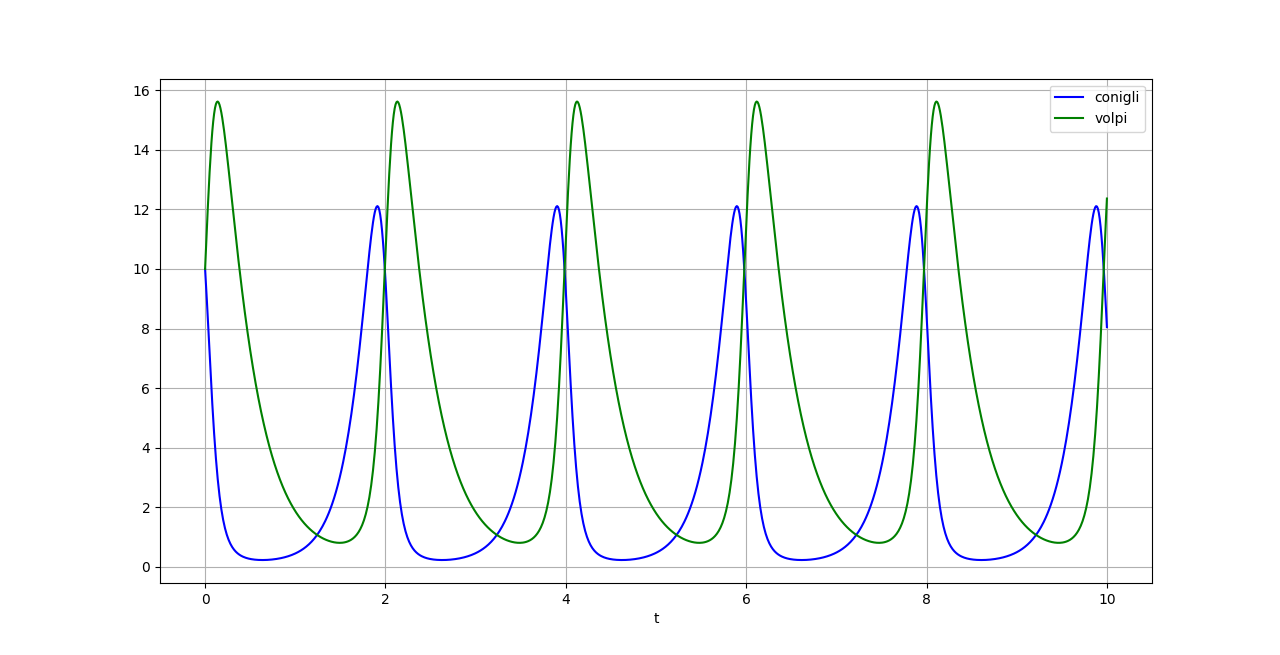
\includegraphics[width=0.4\textwidth]{figures/Volpi-Conigli.png}
\caption{\scriptsize Andamento delle soluzioni (\href{https://github.com/dodogabrie/Sistemi-Complessi/blob/master/python-project/lezione1/volpi_conigli.py}{Link al codice})}
    \label{fig:conigli}
\end{figure}
\noindent
Per una trattazione più rigorosa è necessario notare che le variabili in gioco non sono continue ma bensì discrete (numero di individui di popolazioni).\\
Si passa quindi ad una descrizione probabilistica del sistema che ci porta alla relativa Master Equation.
\begin{center}
    $P(\sigma, t) \in \mathbf{R}$: Probabilità di avere $\sigma \equiv (x,y)\in \mathbf{N}^2$ al tempo $t$.
\end{center}
Inseriamo l'ipotesi di Markov, ovvero che la probabilità che avvenga una transizione tra gli stati del sistema $\sigma \rightarrow \sigma'$ non dipenda dal tempo.
\begin{center}
    $P_r(\sigma\rightarrow\sigma')$: Probabilità di transizione indipendente da $t$.
\end{center}
Dato il sistema al tempo $t$ le probabilità di transizione in un intervallo $\Delta t$ sono:
\[\begin{aligned}
    &P_r(x\to x+1, y) = k_1 c x \Delta t\\
    &P_r(x\to x-1, y \to y+1) = k_2xy\Delta t\\
    &P_r(x\to x,y\to y-1) = k_3 y \Delta t\\
    &P_r(x\to x,y\to y) = 1 - \Delta t \left(k_1cx+ k_2xy + k_3 y\right)
.\end{aligned}\]
Possiamo esprimere la variazione nel tempo della distribuzione di probabilità $P$ tramite le quantità $P_r$:
\begin{redbox}{Esempio di Master Equation}
    Si usa la semplificazione $x^{\pm} \equiv x \pm 1$.
    \begin{equation}
        \begin{aligned}
	    &\frac{P(x,y,t+\Delta  t) - P(x,y,t)}{\Delta  t}  =\\
	    & \quad P_r(x^-\to x, y) \cdot P(x^-,y,t) +\\
	    & \quad P_r(x^+\to x, y^-\to y) \cdot P(x_+,y^-,t) + \\
	    & \quad P_r(x\to x, y^+\to y) P(x,y^+,t) + \\
	    & \quad - \left[1-P_r(x\to x, y\to y)\right]\cdot P(x,y,t) 
        \end{aligned}
    \end{equation}
\end{redbox}
\noindent
Il termine di destra esprime la probabilità di ingresso nello stato $\sigma = (x,y)$ meno la probabilità di uscita da tale stato.
\paragraph{Modello SIR}
Il modello SIR può essere utilizzato per descrivere una situazione pandemica. Gli individui di una popolazione presi in analisi sono:
\begin{itemize}
    \item Suscettibili: $S$.
    \item Infetti: $I$.
    \item Immuni (dopo la malattia): $R$.
\end{itemize}
\[
    \begin{cases}
    S_{n+1} = S_n - \alpha S_n I_n \Delta t\\
    I_{n+1} = I_n + (\alpha S_n I_n - \gamma I_n) \Delta t\\
    R_{n+1} = R_n + \gamma I_n \Delta t
    \end{cases}
\]
Per scrivere la Master Equation si osserva quali sono i termini guidano le transizioni tra i vari stati del sistema:
\[\begin{aligned}
    &P_r(S\to S^-, I \to I^+, R) = \alpha S I \Delta t\\
    &P_r(S, I \to I^-, R \to R^+) = \gamma I \Delta t
.\end{aligned}\]
In modo analogo a quanto fatto per l'esempio precedente si arriva alla seguente equazione:

\begin{align*}
    P(\sigma, &t + \Delta t) = P(\sigma, t) + \\
     + \Delta t &\left[ P(S^+, I^-, R, t) P_r(S^+\to S, I^- \to I, R) + \right.\\
		& \left.+ P(S, I^+, R^-, t) P_r(S, I^+ \to I, R^-\to R) \right] + \\
     - \Delta t & P(\sigma, t) \left[ P_r(S\to S^-, I \to I^+, R) \right. + \\
		& \qquad \qquad \left.+ P_r(S, I\to I^-, R\to R^+)\right].
\end{align*}
A differenza del caso precedente questo sistema ha una configurazione di equilibrio (quando tutti hanno preso il COVID-19 ad esempio).
\paragraph{Rumore shot}%
Ipotizziamo di avere un cavo di rame attraversato da corrente elettrica $J$ e chiamiamo $\sigma$ una sezione di tale cavo ortogonale alla direzione di $J$. Il numero di elettroni che attraversano $\sigma$ sarà soggetto a fluttuazioni, tali fluttuazioni caratterizzano il rumore Shot.\\
La variabile stocastica del problema è $t_k$: il tempo di arrivo di un elettrone su $\sigma$. Ogni elettrone contribuisce alla corrente (misurata su $\sigma$) di una quantità che possiamo schematizzare come una scarica di condensatore $F(t-t_k)$:
\[
    F(t) = \begin{cases}
	0	 			&t<0\\
	q \exp\left(-\alpha t\right) 	&t \ge 0
    \end{cases}
\] 
La corrente totale sarà data dalla somma degli elettroni che arrivano su $\sigma$ per ciascun tempo stocastico $t_k$:
\[
    I(t) = \sum_{t_k}^{} F(t-t_k) 
.\] 
Cerchiamo la Master equation per questo sistema, partiamo dall'ipotesi che in un dato intervallo di tempo $\Delta t$ la probabilità che il numero di elettroni che attraversano $\sigma$ passi da $n$ a $n+1$ sia:
\[
    P(n\to n+1, \text{nell'intervallo }\Delta  t) = \lambda \Delta t
.\] 
Notiamo che gli elettroni scorrono in un'unica direzione, quindi il numero di elettroni che attraversa $\sigma$ può solo aumentare.\\
Il termine della Master Equation $P(n, t + \Delta t)$ si scrive come somma di:
\begin{itemize}
    \item Probabilità di avere già $n$ elettroni al tempo $t$ e che nell'intervallo $\Delta t$ non succeda niente:
	\[
	    (1-\lambda \Delta t) P(n, t)
	\]
    \item La probabilità che al tempo $t$ si hanno $n-1$ elettroni e che nell'intervallo $\Delta t$ ne arrivi un altro:
	\[
	    \lambda \Delta t P(n-1, t)
	\]
\end{itemize}
Quindi mettendo tutto insieme:
\[
    P_n(t+\Delta  t) = \left(1-\lambda\Delta t\right)P_n(t) + \lambda\Delta t  P_{n-1}(t)\implies 
\] 
\[
	\frac{P(n, t+\Delta  t) - P(n,t)}{\Delta t} = \lambda\left[P(n-1,t) -P(n,t)\right] 
.\] 
Che è proprio l'equazione cercata. Vediamo adesso un metodo di risoluzione di questo tipo di equazione.

%%%%%%%%%%%%%%%%%%%%%%%%%%%%%%%%%%%%%%%
%  Metodo della funzione generatrice  %
%%%%%%%%%%%%%%%%%%%%%%%%%%%%%%%%%%%%%%%
\subsection{Metodo della funzione generatrice}%
\label{subsec:fgen_met}
Per risolvere il problema introduciamo la funzione generatrice $G(s,t)$:
\[
    G(s,t) =\sum_{n}^{} s^nP(n,t) 
.\] 
Sostituendo nella master equation del problema precedente nel limite di $\Delta t \to 0$ si ha:
\[
    \frac{\partial G(s,t)}{\partial t} = \lambda (s-1) G(s,t)
.\] 
\[
     \implies  G(s,t) = \exp\left(\lambda (s-1) t\right)G(s,0) 
.\] 
Gli elettroni arrivano per $t\ge 0$, infatti si deve avere che: 
\[
    \begin{cases}
	&P(0,0)=1\\
	&P(n,0) = 0
    \end{cases}
    \ \forall n \implies  G(s,0) = 1 
.\] 
\[\begin{aligned}
    &G(s,t) = e^{\lambda (s-1) t} = \sum_{}^{} s^n P(n,t) \implies  \\
    &\sum e^{-\lambda t} e^{\lambda s t} = \sum_{}^{} e^{-\lambda t}\frac{\left(\lambda ts\right)^n }{n!}  = \sum_{}^{} s^nP(n,t) 
.\end{aligned}\]
In cui si è sfruttato la serie dell'esponenziale $e^{\lambda st}$.
\begin{redbox}{Distribuzione di Poisson}
    \[
	P(n,t)= e^{-\lambda t}\frac{\left(\lambda t\right)^{n}}{n!}
    .\] 
    Dove $P(n,t)$ è la probabilità che al tempo $t$ ci siano $N(t) =n$ elettroni nel sistema.
\end{redbox}
\noindent
Procediamo con il calcolo della corrente, se $N$ è il numero di elettroni arrivati all'istante $t$ allora possiamo definire la quantità:
\[
    \mu(t) \equiv 
    \frac{\text{d} N}{\text{d} t} 
    = \sum_k\delta (t-t_k)  
\] 
Dove $t_k$ è il tempo (random) in cui arriva un elettrone.
Passiamo al continuo nei tempi di arrivo degli elettroni e riscriviamo la corrente come:
\[\begin{aligned}
    I(t) =& \int dx F(t-x) \mu(x) =\\
	 =&\int_{- \infty}^{t} q \exp\left(-\alpha (t-x) \right) \frac{\text{d} N}{\text{d} x} dx 
.\end{aligned}\]
La difficoltà dell'espressione sta nel fatto che $N(t)$ è una funzione a gradini con i gradini che arrivano in modo stocastico nel tempo.\\
Si deriva a destra e sinistra rispetto al tempo ed si integra per parti:
\[\begin{aligned}
    \frac{\text{d} I}{\text{d} t} &= \left[q\exp\left(-\alpha (t-x)\right)\left. \frac{\text{d} N}{\text{d} t}\right]  \right|_{x=t} + \\
				   &\qquad +\int_{-\infty}^{t} \left(-\alpha q\right)\exp\left(-\alpha (t-x)\right)\frac{\text{d} N}{\text{d} x} dx =\\
				   &= q\mu (t) - \alpha I(t) 
.\end{aligned}\]
\begin{redbox}{Equazione stocastica differenziale}
 \[
    \frac{\text{d} I}{\text{d} t} = -\alpha I(t) + q\mu (t) 
.\]    
\end{redbox}
\noindent
Il termine in $\mu$ dipende dalla sequenza casuale di $\delta(t-t_k)$, ognuna di queste può dare soluzioni differenti.\\ 
Rispetto al moto Browniano visto in precedenza, in cui si aveva che $f(\Delta) = f(-\Delta)$, adesso abbiamo un processo che evolve solo in avanti.\\
L'idea per risolvere il problema è di interpolare l'andamento di $N$ con un moto browniano, prendendo la media e le fluttuazioni del termine stocastico.
Essendo il termine in $\mu$ la derivata di un processo poissoniano abbiamo le seguenti proprietà:
\[\begin{aligned}
    &\left<\mu dt\right>=\left<dN\right> = \lambda dt\\
    & \left<\left(\lambda dt - \mu dt\right)^2\right> = \lambda dt
.\end{aligned}\]
Si cerca di scrivere questo processo stocastico (unilaterale) come un processo di Langevin, quindi si definisce una nuova variabile stocastica $d\eta = dN - \lambda dt$.
\[
    dN = \lambda dt + d\eta	
.\] 
Questo equivale a scomporre il processo a salti $dN$ in un drift lineare ($\lambda dt$) ed una fluttuazione stocastica ($d\eta$).\\
Il differenziale della corrente si scrive come:
\[
    dI(t) = \left(\lambda q-\alpha I\right)dt+ qd\eta (t) 
.\] 
In questo modo la variabile stocastica $d\eta$ gode delle seguenti proprietà:
\begin{itemize}
    \item $\left<d\eta \right> = 0$
    \item $\left<d\eta^2 \right> = \lambda dt$
    \item $\left<I d\eta \right> = 0$
\end{itemize}
\[
    \frac{\text{d} }{\text{d} t} \left<I\right> = \lambda q -\alpha\left<I\right>
.\] 
Il risultato stazionario per l'equazione è:
\[
    \left<I\right>_{\infty}=\frac{\lambda q}{\alpha}
.\] 
Procediamo con una ipotesi sbagliata: trascurare le fluttuazioni nel seguente termine
\begin{equation}
    \left(I+dI\right)^2 \approx I^2 + 2IdI	\label{eq:baddiff}
\end{equation}
Quindi con il risultato che dovrebbe esser noto sui differenziali: $d\left(I^2\right) = 2IdI$, se assumiamo questo e moltiplichiamo a destra e sinistra per $\left<I\right>$ nella equazione   per la corrente otteniamo:
\[
    \frac{1}{2}\frac{\text{d} }{\text{d} t} \left<I^2\right>= \lambda q\left<I\right>-\alpha\left<I^2\right>
.\] 
Che ci porta a concludere che:
\[
    \left<I^2\right>_{\infty} = \frac{\lambda q}{\alpha}\left<I\right>_{\infty} = \left(\left<I\right>_{\infty}\right)^2
.\] 
Otteniamo quindi un paradosso, la corrente ha varianza nulla:
\[
  \left<I^2\right>-\left<I\right>^2 = 0  
.\] 
Questo significherebbe che la "larghezza" del moto Browniano è nulla, quindi la corrente sarebbe costante e continua.\\
L'errore è dovuto al differenziale \ref{eq:baddiff}, infatti il termine trascurato vale:
\[
    \left<dI^2\right> = \left<q^2d\eta^2\right> = q^2\lambda dt
.\] 
Che è anch'esso di prim'ordine nel tempo! L'equazione corretta sarebbe allora:
\[
    \frac{1}{2}\frac{\text{d} }{\text{d} t} \left<I^2\right>= \lambda q\left<I\right>-\alpha\left<I^2\right> + q^2\lambda + O(dt)
.\]
\newpage

\section{Lezione 2}%
\label{sub:Lezione 2}

\subsection{Esempi di Master equation}%
\begin{itemize}
    \item Rumore shot.
    \item Rumore Jonshon
\end{itemize}
Prendiamo il rumore Shot, questo si basa sul fatto che la corrente non è proprio continua, chiamiamo $t_k$ il tempo di arrivo di un elettrone:
\[
    I(t) = \sum_{t_k}^{} F(t-t_k) 
.\] 
Mentre $F(t-t_k)$ è una funzione a pinna di squalo. Cerchiamo la Master equation per questo sistema:
\[
    P(n\to n+1, \text{in }\Delta  t) = \lambda \Delta tP_n(t) 
.\] 
Visto che possiamo riscrivere la probabilità di avere $n$ elettroni al tempo $t+\Delta t$ come: 
\[
    P_n(t+\Delta  t) = \left(1-\lambda\Delta t\right)P_n(t) + \lambda\Delta t 
.\] 
Si ottiene:
\[
    \frac{P(n, t+\Delta  t) - P(n,t)}{\Delta t} = \lambda (P(n-1,t) -P(n,t)) 
.\] 
\subsection{Metodo della funzione generatrice}%
Possiamo risolvere questa equazione utilizzando una tecnica standard: la funzione generatrice $G(s,t)$:
\[
    G(s,t) =\sum_{}^{} s^nP(n,t) 
.\] 
Sostituendo nella master si ha:
\[
    \frac{\partial G(s,t)}{\partial t} = \lambda (s-1) G(s,t) 
.\] 
Che si risolve con il risultato:
\[
    G(s,t) = \exp\left(\lambda (s-1) t\right)G(s,0) 
.\] 
Gli elettroni arrivano per $t\ge 0$, infatti si deve avere che: $P(0,0)=1$, $P(n,0) = 0 \ \forall n$, queste condizioni iniziali ci portano a $G(s,0) = 1$.
\[\begin{aligned}
    G(s,t) =& e^{\lambda (s-1) t}G(s,0) = \sum_{}^{} s^n P(n,t) \implies  \\
		&\sum_{}^{} e^{-\lambda t}\frac{\left(\lambda ts\right)^n }{n!}G(s,0)  = \sum_{}^{} s^nP(n,t) 
.\end{aligned}\]
In cui si è sfruttato la serie dell'esponenziale $e^{\lambda st}$.
\begin{redbox}{Distribuzione di Poisson}
    \[
	P(n,t)= e^{-\lambda t}\frac{\left(\lambda t\right)^{n}}{n!}
    .\] 
    Dove $P(n,t)$ è la probabilità che al tempo $t$ abbiamo $N(t) =n$ elettroni.
\end{redbox}
\noindent
Tornando alla corrente dobbiamo trovare un modo per contare gli elettroni:
\[
    \mu (t) = \frac{\text{d} N}{\text{d} t} \quad
    \begin{cases}
	&0 \quad \text{di solito}\\
	&\delta (t-t_k) \quad \text{Arriva e$^-$ al tempo }t_k
    \end{cases}
\] 
Dove ricordiamo che $t_k$ è random.
Quindi abbiamo che: 
\[
    \mu (t) = \sum_{k}^{} \delta (t-t_k) 
.\] 
Allora possiamo riscrivere la corrente con un integrale sfruttando le $\delta$:
\[
    I(t) = \int dx F(t-t_k) \mu (x) 
.\] 
Prendendo come $F$ modello la funzione:
\[
    F(t) = \begin{cases}
        0 \quad t<0\\
	q \exp\left(-\alpha t\right) \quad t \ge 0
    \end{cases}
.\] 
Otteniamo per la corrente:
\[
    I(t) = \int_{- \infty}^{t} q \exp\left(-\alpha (t-x) \right) \frac{\text{d} N}{\text{d} x} dx 
.\] 
Adesso dobbiamo risolvere il problema che $N(t)$ è una funzione a salti irregolari tra loro. Vediamo l'equazione differenziale per $I(t)$.
\[\begin{aligned}
    \frac{\text{d} I}{\text{d} t} =& q\exp\left(-\alpha (t-x)\right)\left.\dot{N}\right|_{x=t} + \\
				   &+\int_{-\infty}^{t} \left(-\alpha q\right)\exp\left(-\alpha (t-x)\right)\dot{N}dx 
.\end{aligned}\]
Risolvendo a sinistra ed usando le definizioni ci si riduce a:
\begin{redbox}{Equazione stocastica differenziale}
 \[
    \frac{\text{d} I}{\text{d} t} = -\alpha I(t) + q\mu (t) 
.\]    
\end{redbox}
Il termine in $\mu$ dipende dalla sequenza casuale di $\delta$, ogni sequenza casuale diversa ci può dare soluzioni diverse.\\
L'idea per risolvere il problema è di interpolare l'andamento di $N$ con un moto browniano, prendendo la media e le fluttuazioni del termine stocastico.
Essendo il termine in $\mu$ la derivata di un processo poissoniano abbiamo le seguenti proprietà:
\[\begin{aligned}
    &\left<\mu dt\right>=\left<dN\right> = \lambda dt\\
    & \left<\left(\lambda dt - \mu dt\right)^2\right> = \lambda dt
.\end{aligned}\]
Si ha un termine di fluttuazioni $d\eta$ tale che:
\[
    dN = \lambda dt + d\eta	
.\] 
Il differenziale della corrente si scrive come::
\[
    dI(t) = \left(\lambda q-\alpha I\right)dt+ qd\eta (t) 
.\] 
Prendendo la media di questa equazione abbiamo che il termine di fluttuazione media a zero:
\[
    \frac{\text{d} }{\text{d} t} \left<I\right> = \lambda q -\alpha\left<I\right>
.\] 
Questa equazione per tempi lunghi da il risultato stazionario:
\[
    \left<I\right>_{\infty}=\frac{\lambda q}{\alpha}
.\] 
Andiamo avanti nel conto con la seguente presa di posizione:
\begin{equation}
    \left(I+dI\right)^2 \approx I^2 + 2IdI	\label{eq:baddiff}
\end{equation}
Quindi con il risultato che dovrebbe esser noto sui differenziali: $d\left(I^2\right) = 2IdI$, se assumiamo questo e moltiplichiamo a destra e sinistra per $\left<I\right>$ nella equazione   per la corrente otteniamo:
\[
    \frac{1}{2}\frac{\text{d} }{\text{d} t} \left<I^2\right>= \lambda q\left<I\right>-\alpha\left<I^2\right>
.\] 
Che ci porta a concludere che:
\[
    \left<I^2\right>_{\infty} = \frac{\lambda q}{\alpha}\left<I\right>_{\infty} = \left(\left<I\right>_{\infty}\right)^2
.\] 
Otteniamo quindi un paradosso, la corrente ha varianza nulla:
\[
  \left<I^2\right>-\left<I\right>^2 = 0  
.\] 
Questo significherebbe che la "larghezza" del moto Browniano è nulla, quindi la corrente sarebbe costante e continua.\\
L'errore è dovuto al differenziale \ref{eq:baddiff}, infatti il termine trascurato vale:
\[
    \left<dI^2\right> = \left<q^2d\eta^2\right> = q^2\lambda dt
.\] 
Che è anch'esso di prim'ordine nel tempo! L'equazione corretta sarebbe allora:
\[
    \frac{1}{2}\frac{\text{d} }{\text{d} t} \left<I^2\right>= \lambda q\left<I\right>-\alpha\left<I^2\right> + q^2\lambda
.\]

\section{Funzione caratteristica e Momenti Fattoriali}%
\label{sub:Lezione 3}
\mylocaltoc
\subsection{Funzione caratteristica e cumulanti}%
\label{sub:Funzione caratteristica}
Sia $\vect{x}$ una variabile random con distribuzione di probabilità $P(\vect{x})$, la funzione caratteristica della distribuzione è la sua trasformata di Fourier:
\begin{redbox}{}
    \[
	\phi (\vect{s}) = \int d\vect{x} P(\vect{x}) e^{i \vect{x}\cdot \vect{s}}
    .\] 
\end{redbox}

\begin{exmp}[Distribuzione Gaussiana]
 \[\begin{aligned}
    &P(x) = \frac{e^{-x^2 / 2 \sigma^2}}{\sqrt{2\pi\sigma^2}} 
    &\implies&
    &\phi (s) = e^{-\sigma^2s^2 / 2}
.\end{aligned}\]
\end{exmp}

\begin{exmp}[Distribuzione uniforme]
\[
    P(x) = 
    \begin{cases}
	1 & x \in \left[-\frac{1}{2}, \frac{1}{2}\right]\\
	0 & \text{Altrimenti}
    \end{cases}
\] 
\[
    \phi (s) = \int_{-1 /2}^{1 /2} e^{ixs}dx = \frac{2}{s}\sin\left(\frac{s}{2}\right)  
.\] 
\end{exmp}

\subsubsection{Proprietà della funzione caratteristica}%
\label{ssub:Proprietà della funzione caratteristica}
\begin{enumerate}
    \item $\left|\phi (0) \right|= 1 $.
    \item $\phi (s) $ è continua.
    \item Se $\exists \left<x^n\right>$ allora: 
	\[
		\left<x^n\right> = \left(-i\right)^n \left.\frac{\partial ^n}{\partial s^n} \phi (s)\right|_{s=0} 
	.\] 
    \item Una sequenza di distribuzioni converge ad una distribuzione limite $\iff$ converge la sequenza di funzioni caratteristiche.
    \item Dato $\vect{x} = \left(x_1, \ldots, x_n\right)$ con $x_i$ indipendenti $\forall i$ allora:
	\[ 
	    \phi (s_1, s_2, \ldots) = \prod_{i=1}^{n} \phi (s_i)  
	\]
    \item Se $y = \sum_{i}^{} x_i$ con $x_i$ indipendenti, allora:
	\[
	    \phi (s) = \left<e^{isy}\right> = \prod_{i}^{} \phi_i(s)  
	.\] 
	\begin{exmp}
	    Se $y = x_1 + x_2$ ho che:
	    \[
		P(y) = \int P(x_1) P(y-x_1) dx_1
	    .\] 
	    Allora per le proprietà della trasformata di una convoluzione:
	    \[
		\phi (s) = \phi_1(s) \phi_2(s) 
	    .\] 
	\end{exmp}
\end{enumerate}
\begin{exmp}[Testa o Croce]
    Prendiamo una distribuzione che corrisponda alla probabilità del set di eventi ["testa","croce"] dopo il lancio di una moneta:
    \[
        P(x) = \frac{1}{2}\left( \delta(x-1) + \delta(x+1) \right) 
    \]
    Calcoliamo la funzione caratteristica di tale distribuzione:
    \[
	\phi(s) = \int P(x) e^{isx} dx = \frac{1}{2}\left[ e^{is} + e^{-is} \right] 
    \]
    Ipotizziamo di fare $n$ lanci di moneta e di voler inferire tramite la funzione caratteristica quale sarà la distribuzione di probabilità finale. \\
    Stiamo parlando della probabilità di una somma di eventi indipendenti, quindi per quanto visto in precedenza si ha che:
    \[
	\phi_n(s) = \left[ \phi(s) \right] ^n = \frac{1}{2^n} \left( e^{is} + e^{-is} \right)^n 
    \]
    Si sfrutta la formula binomiale (somma di elementi elevati alla $n$):
    \[
	\phi_n(s) = \frac{1}{2^n}\sum_{k = 0}^{n}\binom{n}{k} e^{is(n-2k)}
    \]
    La trasformata inversa assume la forma di una somma di delta di Dirac che dovrebbero convergere ad una Gaussiana nel limite di $n\to\infty$:
    \[
	P(x) = \frac{1}{2\pi}\int ds \phi_n(s) e^{-ixs} = \frac{1}{2^n} \sum_{k = 0}^{n} \binom{n}{k}\delta(n-2k)
    \]
\end{exmp}
\subsubsection{Cumulanti della funzione caratteristica.}%
\label{sub:Sviluppo in cumulanti di phi}
\begin{redbox}{Funzione generatrice dei cumulanti}
   \[
       \Phi(s) = \ln (\phi (s) ) 
   .\]  
\end{redbox}
\noindent
Si potrebbe dimostrare che la funzione generatrice si esprime in modo generale in funzione di quantità definite come cumulanti:
\[\begin{aligned}
    \Phi = \sum_{r=1}^{\infty} i^r \sum_{\left\{m\right\}}^{} 
    \left<\left< x_1^{m_1}x_2^{m_2}\ldots\right>\right> 
    \prod_{i=1}^{\infty} \frac{s_i^{m_i}}{m_i!\,}\delta (r-\sum_{i=1}^{r} m_r) 
.\end{aligned}\]
Dove i termini tra le parentesi $\left<\left< x_i^{m_i}\right>\right>$ sono i cumulanti. Prendiamo ad esempio lo sviluppo dei primi due:
\[\begin{aligned}
    & \left<\left<x_1\right>\right> = \left<x_1\right> \sim \text{Media}\\
    & \left<\left<x_1 x_2 \right>\right> = \left<x_1x_2\right> - \left<x_1\right>\left<x_2\right> \sim \text{ Covarianza}
.\end{aligned}\]
Consideriamo adesso i cumulanti per una stessa variabile stocastica ($x_i = x_j $ $\forall i, j$), che chiameremo in questo contesto anche \texttt{Momenti}.
\begin{greenbox}{Cumulanti di processo Gaussiano.}
   I cumulanti per un processo Gaussiano sono tutti nulli per $n\ge 3$.
   \[
       \left<\left<x^n\right>\right> = 0 \quad \forall n \ge  3
   .\] 
\end{greenbox}
\begin{exmp}[Cumulante quarto per Gaussiana]
    \[\begin{aligned}
	\left<\left<x^4\right>\right> =& \left<x^4\right>-4\left<x^3\right>\left<x\right>+\\
					&-3\left<x^2\right>^2 + 12\left<x^2\right>\left<x\right>^2-6\left<x\right>^4
    .\end{aligned}\]
    Possiamo dimostrare che $\left<\left<x^4\right>\right> = 0$ valutando $\frac{d}{dx}\left<x^3\right>$:
    \[
        \int_{-\infty}^{\infty} \frac{\text{d} }{\text{d} x} \left\{x^3 \exp\left(\frac{-x^2}{2\sigma^2}\right)\right\} dx = 0 
    .\] 
    Questa si azzera perché la Gaussiana si annulla in $x = \pm \infty$, la precedente equazione può essere riscritta tramite le regole della derivata composta:
    \[
        \int\left(3x^2\exp\left(-\frac{x^2}{2\sigma^2}\right) - 
		\frac{x^4}{\sigma^2}\exp\left(- \frac{x^2}{2\sigma^2}\right) \right)dx = 0 
    .\] 
    \[
	\left<x^4\right> = 3\sigma^2\left<x^2\right> = 3 \left(\sigma^2\right)^2
    .\] 
    Inserendo nella equazione per il cumulante quarto si annullano tutti i termini (per semplicità abbiamo preso una gaussiana a media nulla $\left<x\right>=0$ ) .
\end{exmp}
\noindent
In generale questa cosa non funziona, non è possibile esprimere i cumulanti in funzione di altri cumulanti di ordine inferiore per ogni distribuzione.

\subsection{Teorema del limite centrale}%
\label{sub:Teorema del limite centrale}
\begin{redbox}{Teorema del limite centrale}
   La somma di variabili stocastiche aventi media e varianza definita tende ad una Gaussiana. 
\end{redbox}
\noindent
Sia $\left\{x_i\right\}$ una variabile random con distribuzione di probabilità $P_i(x_i)$, il teorema richiede che i primi due momenti siano definiti:
\[\begin{aligned}
    & \left<x_i\right> = 0; &&
    & \text{var}\left\{x_i^2\right\} = b_i^2
.\end{aligned}\]
Si definiscono le seguenti quantità:
\[\begin{aligned}
    & s_n = \sum_{i=1}^{n} x_i;
    &&
    &\sigma_n^2 = \sum_{i=1}^{n} b_i^2
.\end{aligned}\]
Se le code della $s_n$ si annullano in modo "rapido" secondo la seguente equazione:
\[
    \lim_{n \to \infty} 
    \left[\frac{1}{\sigma_n^2} \sum_{i=1}^{n} \int\limits_{\left|x\right|>t\sigma_n}^{} dx x^2_i P_i(x)  \right] 
    = 0 \qquad \forall t>0
.\] 
Se ne conclude che $s_n/\sigma_n$ tende ad una gaussiana di media nulla e varianza unitaria.
\[
    \tilde{s}_n = s_n /\sigma_n \to G \qquad \mbox{Per} \ n \to \infty
.\] 
\begin{exmp}[Distribuzione che non tende ad una Gaussiana]
    Una somma di variabili stocastiche distribuite secondo una Lorenziana non tende ad una Gaussiana perché il suo momento secondo diverge.
\end{exmp}
\noindent
\subsubsection{Teorema di Chebyshev}%
\label{subsub:Teorema di Chebyshev}
Si cerca di quantificare quanto velocemente una distribuzione tenda alla Gaussiana.\\
Definiamo la funzione:
\[
    F_n(t) \equiv \int_{-\infty}^{t} \tilde{P}(\tilde{s}_n)d\tilde{s}_n;  \qquad \phi (t) = \lim_{n \to \infty} F_n(t) 
.\] 
Dove $\tilde{P}$ è la distribuzione dei $\tilde{s}_n$, che tiene di conto che ad ogni step $n$ cambia la normalizzazione necessaria per essere una probabilità.
\begin{redbox}{Teorema di Chebyshev}
    \[
	F_n-\phi (t) \sim \frac{e^{-t^2 /2}}{\sqrt{2\pi}}\left[\frac{Q_1(t)}{n^{1 /2}} + \frac{Q_2(t)}{n} + \ldots\right]
    .\] 
    In cui i $Q_i$ sono i polinomi di Chebyshev-Hermite, legati ai momenti di $\left\{x_i\right\}$.
\end{redbox}
\noindent
Prendiamo ad esempio $Q_1(t)$:
\[
    Q_1(t) \propto \frac{\left<\left(x-\left<x\right>\right)^3\right>}{\sigma^3}
.\] 
la quantità a destra è legata al momento terzo di $\left\{x_i\right\}$, di conseguenza è nulla nel caso gaussiano (e lo sono anche tutte le restanti $Q_i$).\\
In conclusione le distribuzioni tendono ad una Gaussiana nelle ipotesi del teorema del limite centrale come $1 / \sqrt{n} $.

\subsection{Momenti fattoriali}%
\label{sub:Momenti fattoriali}
I momenti fattoriali di una distribuzione $f$ sono definiti nel seguente modo:
\begin{redbox}{Momenti fattoriali}
    \[
	\left<n^r\right>_f = \left<n\cdot (n-1) \cdot \ldots \cdot (n-r+1) \right>
    .\] 
\end{redbox}
\noindent
\subsubsection{Momenti fattoriali della distribuzione di Poisson}%
\label{subsub:Momenti fattoriali della distribuzione di Poisson}
Prendiamo la distribuzione:
\[
	P(n) = e^{-\lambda } \frac{\lambda^n}{n!\,}
.\] 
\begin{exmp}[Poisson con $r=2$.]
    Sia $f$ Poissoniana:
   \[\begin{aligned}
       \left<x^2\right>_f=\left<x\left(x-1\right)\right>_f =& \sum_{x = 0}^{\infty} x\left(x-1\right)e^{-\lambda} \frac{\lambda^x}{x!\,} = \\
       =& \lambda^2 \sum_{x = 0}^{\infty}  e^{-\lambda} \frac{\lambda^{x-2}}{\left(x-2\right)!} = \lambda^2
   .\end{aligned}\]
   L'ultimo passaggio lo si ottiene dal fatto che l'indice della sommatoria può essere traslato e che tale sommatoria si estende ad $\infty$, quindi la somma corrisponde a $\left<f\right> \equiv 1$.
\end{exmp}
\noindent
Iterando questa procedura si ottiene:
\begin{bluebox}{Momenti fattoriali per distribuzione di Poisson}
 \[
    \left<x^r\right>_f = \lambda^r
.\]    
\end{bluebox}
\noindent

\subsection{Funzione generatrice generalizzata.}%
\label{subsub:Funzione generatrice generalizzata.}

\begin{redbox}{Funzione generatrice}
    \[
	G(s) = \sum_{n=0}^{\infty} s^n P(n) = \left<s^n\right>
    .\] 
\end{redbox}
\noindent
Possiamo ottenere la $G(s)$ a partire dalla funzione caratteristica:
\[
    G(s) = \phi (-i\ln s) 
.\] 
Grazie a questa possiamo esprimere i momenti fattoriali nel seguente modo:
\[
    \left<x^n\right>_f = \left[\frac{\partial^n}{\partial s^n} G(s)\right]_{s=1}
.\] 
\begin{bluebox}{Funzione generatrice dei cumulanti fattoriali}
    \[
	g(s) \equiv \ln (G(s)) = \sum_{r=1}^{\infty} \left<\left<x^r\right>\right>_f \frac{\left(s-1\right)^r}{r!}
    .\] 
\end{bluebox}
\noindent
I cumulanti fattoriali, come quelli visti nella sezione precedente, sono tabulati per ciascuna distribuzione.
\begin{exmp}[Funzione generatrice per Poissoniana]
    \[\begin{aligned}
	G(s) =& \sum_{n=1}^{\infty} s^n e^{-\lambda} \frac{\lambda^n}{n!\,} =\\
	=& e^{-\lambda}\sum_{n=1}^{\infty} \frac{\left(s\lambda\right)^n}{n!\,} =  e^{\lambda (s-1) }
     .\end{aligned}\]
     Che è lo stesso risultato ottenuto nella \ref{subsec:fgen_met}.
     Per Poisson si ha quindi che:
     \[
         \left<\left<x^r\right>\right>_f = 0 \quad \forall r \ge  2
     .\] 
\end{exmp}
\noindent
\clearpage

\section{Lezione 4}%
\label{sub:Lezione 4}
\subsection{Continuità dei processi stocastici}%
\label{sub:Continuità dei processi stocastici}
\begin{defn}[Processo continuo]
    Un processo stocastico si dice continuo se $\forall \epsilon > 0$: 
    \[
	\lim_{\Delta t \to 0} \frac{1}{\Delta t}\int\limits_{\Sigma_\epsilon}   dx_1 P_{1|1}(x_1, t + \Delta t | x_2, t) = 0
    .\] 
    \[
        \Sigma_\epsilon : \left\{ \left|x_1-x_2\right|>\epsilon\right\}
    .\] 
\end{defn}
\noindent
In pratica serve che il cammino descritto dal processo sia continuo, la distanza tra due punti del processo deve andare a $0$ più rapidamente di $\Delta t$.\\
I processi Markoviani non sono necessariamente continui:
\begin{exmp}[Pollaio]
    Il numero di uova prodotte in un pollaio in un giorno può essere schematizzato come processo markoviano: dipende soltanto dal numero di galline presenti nel pollaio il giorno prima.\\
    Questo processo non può essere continuo: è possibile mandare il $\Delta t$ a $0$ ma non possiamo fare altrettanto con $x$, ovvero il numero di uova. Infatti in questo caso il numero di uova è discreto. \\
    In generale i processi a salti discreti non possono essere continui.
\end{exmp}
\noindent
\begin{exmp}[Moto Browniano]
    Calcoliamo l'equivalente della $P_{1|1}$ nel moto Browniano, nella lezione $1$ abbiamo visto che:
    \[
	P(x, t+\Delta t) = \int P(x-\Delta, t) f(\Delta) d\Delta
    .\] 
    Con $f(\Delta)$: probabilità di fare un salto lungo $\Delta$ nell'intervallo di tempo $\Delta t$.\\
    Definendo la quantità $y = x-\Delta$ intuitivamente la $f(\Delta)$ corrisponde alla probabilità condizionata:
    \[
	f(\Delta) = P_{1|1}(x, t+\Delta t| y, t) 
    .\] 
    Essendo un oggetto Gaussiano la $f(\Delta)$ avrà la seguente struttura:
    \[
	f(\Delta) = \frac{1}{\sqrt{4\pi D\Delta t} }\exp\left(-\frac{1}{4D\Delta t} \left(x-y\right)^2  \right) 
    .\] 
    In altre parole $f(\Delta)$ è proprio un propagatore.\\
    Inserendo questo oggetto nella definizione di processo continuo si vede che l'uguaglianza al limite è soddisfatta, quindi il moto Browniano è un processo continuo.
\end{exmp}
\noindent
\begin{exmp}[Moto di Cauchy]
    Il moto di Cauchy presenta una struttura per la probabilità di salto (condizionata) del seguente tipo:
    \[
	P_{1|1}(x,t+\Delta t| z , t)  = \frac{\Delta t}{\pi} \frac{1}{\left(x-z\right)^2 + \left(\Delta t\right)^2}
    .\] 
    E si può dimostrare che:
    \[
	\lim_{\Delta t \to 0} \frac{1}{\Delta t}\int\limits_{\Sigma_\epsilon}
	\frac{\Delta t dx}{\pi\left[\left(x-z\right)^2 + \left(\Delta t\right)^2\right]} = \infty
    .\] 
    Di conseguenza il moto di Cauchy non è continuo.
\end{exmp}
\noindent
\begin{figure}[H]
    \centering
    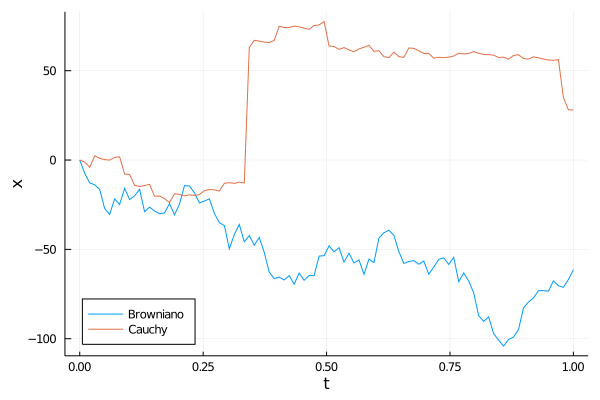
\includegraphics[width=0.4\textwidth]{figures/4_cauchy-brown.png}
    \caption{\scriptsize Processo di Brown e Processo di Cauchy a confronto \href{https://github.com/dodogabrie/Sistemi-Complessi/blob/master/python-project/lezione4/lez4_Cauchy-Brown.ipynb}{Link al codice in Julia}).}
    \label{fig:-fig}
\end{figure}

%%%%%%%%%%%%%%%%%%
%  Chapman form  %
%%%%%%%%%%%%%%%%%%

\subsection{Forma differenziale di Chapman - Kolmogorov}%
\label{sub:Forma differenziale di Chapman - Kolmogorov}
Prendiamo un processo stocastico scomponibile\
\footnote{Ipotesi per cui si può scomporre sul Gardiner}  in una parte continua ed una non continua.\\
Si può dimostrare che un processo di questo tipo è descritto dalla seguente forma differenziale:
\begin{redbox}{Forma di Chapman-Kolmogorov}
    \begin{equation}
    \partial_{t}P(\vect{z},t| \vect{y}, t') = - \Gamma + \Phi
    \label{eq:4_CK}
    \end{equation}
\end{redbox}
\noindent
In cui $\Gamma$ è la parte contenente il processo continuo:
\[\begin{aligned}
    \Gamma = \sum_{i}^{} \partial_{z_i}&\left[ A_i(\vect{z},t) P(\vect{z},t|\vect{y},t') \right] +\\
                         &+\sum_{i,J}^{} \frac{1}{2}\partial^2_{z_iZ_J}\left[ B_{iJ}(z,t) P(\vect{z},t|\vect{y},t') \right]
.\end{aligned}\]
Qui abbiamo un primo termine "deterministico" (con la $A$) che determina soltanto uno spostamento dell'oggetto ed un termine di diffusione (quello in $B$).\\
Nella $\Phi$ abbiamo invece il processo discontinuo:
\[\begin{aligned}
    \Phi = \int  d\vect{x} &\left[\omega (\vect{z}|\vect{x}, t) P(\vect{x},t|\vect{y}, t') \right. + \\
			   & \left. - \omega(\vect{x} | \vect{z}, t)  P(\vect{z},t|\vect{y},t') \right]
.\end{aligned}\]
Il termine $\Phi$ somiglia molto al termine della equazione di Volterra che abbiamo visto nella prima lezione (prob. di trovarsi in $\vect{z}$ è data dalla probabilità di finire in $\vect{z}$ da una posizione $\vect{x}$ diminuito la prob. di scappare in $\vect{x}$ dalla posizione $\vect{z}$).\\
La potenza della equazione è la sua generalità: se sappiamo che un processo è Markoviano (magari per la fisica che ci sta dietro) allora l'equazione di evoluzione delle prob. nel tempo sarà necessariamente quella sopra.
\begin{exmp}[$A=B=0$, quindi $\Gamma =0$]
    \[
        \partial_{t}P = \Phi
    .\] 
    Considerando il rapporto incrementale con passo $\Delta t$:
    \[
	P(z, t+\Delta t|y, t) = P(z,t|y,t) + \Delta t\cdot  \Phi
    .\] 
    Sfruttiamo la proprietà ovvia:
    \[
	P(\vect{z}, t|\vect{t}, t) = \delta (\vect{y}-\vect{z}) 
    .\] 
    Allora possiamo sviluppare l'espressione con $\Delta t$ che tende a $0$ (mettiamoci in una dimensione per semplicità):
    \begin{greenbox}{Soluzione della forma diff. con termini continui}
    \[\begin{aligned}
	P&(z, t + \Delta t| y, t) = \\
				  &= \delta (z-y) \left[1-\Delta t\int dx \omega (x|z) \right] + \Delta t \cdot \omega (z|y) 
    .\end{aligned}\]
    \end{greenbox}
    \noindent
\end{exmp}
\noindent

\subsection{Processo di Wiener}%
\label{sub:Processo di Wiener}
Un processo di Wiener è modellato dalla seguente equazione:
\begin{greenbox}{Equazione per processo di Wiener}
    L'equazione che regola il processo di Wiener è una Fokker-Planck:
    \[
	\frac{\partial }{\partial t} P(\omega,t|\omega_0, t_0) =
	\frac{1}{2}\frac{\partial ^2}{\partial \omega^2} P(\omega, t|\omega_0, t_0) 
    .\] 
\end{greenbox}
\noindent
Inoltre deve esser rispettata la condizione iniziale:
\[
    P(\omega,t_0|\omega_0, t_0) = \delta (\omega-\omega_0) 
.\]
Il processo si può risolvere utilizzando la funzione caratteristica:
\[
    \phi (s, t) = \int d\omega P(\omega, t|\omega_0, t_0) e^{is\omega}
.\] 
Sfruttando le regole della trasformata possiamo riscrivere l'equazione del processo come:
\[
    \frac{\partial \phi }{\partial t} = -\frac{1}{2}s^2\phi
.\] 
\[
    \phi (s, t_0) = \exp (is\omega_0) 
.\] 
La soluzione è nota:
\[\begin{aligned}
    \phi (s) =& \exp\left(-\frac{1}{2}s^2\left(t-t_0\right)\right)\phi (s,t_0)  =\\
    	=&\exp\left(-\frac{1}{2}s^2\left(t-t_0\right) + is\omega_0 \right) 
.\end{aligned}\]
Visto che l'antitrasformata di una Gaussiana è una Gaussiana abbiamo la soluzione nello spazio reale:
\begin{redbox}{Soluzione del processo di Wiener}
    \[
	P(\omega,t|\omega_0, t_0) = 
	\frac{1}{\sqrt{2\pi\left(t-t_0\right)} }
	\exp\left(- \frac{\left(\omega-\omega_0\right)^2}{2\left(t-t_0\right)}\right)
    \] 
\end{redbox}
\noindent
Il processo che abbiamo ottenuto è Gaussiano:
\[
    \left<\omega\right> =  \omega_0
.\] 
\[
    \left<\left(\omega-\omega_0\right)^2\right> = t- t_0
.\] 
\paragraph{Proprietà dei processi di Wiener}%
\label{par:Proprietà dei processi di Wiener}
\begin{itemize}
    \item \'E continuo.
    \item Non è differenziabile, $\forall k$:
	\[\begin{aligned}
	    \text{Prob}&\left(\frac{\left|\omega (t+h) - \omega (t) \right|}{h}> k\right) = \\
		       & = 2 \int_{kh}^{\infty} d\omega  \frac{1}{\sqrt{2\pi  h}} e^{- \omega^2 /2h} 
		       \ \xrightarrow[]{h\to 0} 1
	.\end{aligned}\]
    \item Gli incrementi sono indipendenti:
	\[\begin{aligned}
	    P(&\omega_2, t_2; w_1,t_1; \omega_0,t_0) = \\
	      &= P(\omega_2, t_2|\omega_1,t_1) P(\omega_1, t_1|\omega_0,t_0) P(\omega_0,t_0) 
	.\end{aligned}\]
	Il primo termine dopo l'uguale non dipende da $(\omega_0,t_0)$ perché il processo è Markoviano.
    \item La correlazione: 
    \[
	\left<\omega (t) \omega (s) | \left[\omega_0, t_0\right]\right> = \text{min}(t-t_0, s-s_0) + \omega_0^2
    .\] 
    Che nel caso particolare in cui $\omega_0=t_0=0$ si ha $\left<\omega (t) \omega (s) \right> = s$ se $t>s$.
    \usetikzlibrary{math}
    \tikzmath{\x = 5; \y = 4;}
    \begin{center}
    \begin{tikzpicture}
	 \draw[-stealth] (0,0) --(\x/\y, 0)node[below]{$s$} -- (\x,0) node[right]{$t$};
	 \draw[-stealth] (0,0) --(0,\x/\y)node[left]{$s$} -- (0,\x*2/5) node[above]{$\left<\omega (t) \omega (s) \right>$};
         \draw[thick] 
		  (0,0) node[below]{$0$} -- 
		  (\x/\y,\x/\y)  -- 
		  (\x,\x/\y);
	 \draw[dash dot] 
		  (\x/\y, 0) --
		  (\x/\y, \x/\y);
	\draw[dash dot] 
		  (0,\x/\y) --
		  (\x/\y, \x/\y);

    \end{tikzpicture}
    \end{center}
    \noindent
\end{itemize}
\clearpage

\section{Lezione 5}%
\label{sub:Lezione 5}
\subsection{Processo di Ornstein - Uhlenback}%
\label{sub:Processo di Ornstein - Uhlenback}
Prendiamo in considerazione altri esempi di processi di Markov.
\begin{redbox}{Equazione di Ornstein - Uhlenback}
    \[
	\frac{\partial P}{\partial t} = \frac{\partial }{\partial x} (kxP) + \frac{1}{2}D\frac{\partial ^2}{\partial x^2} P
    .\] 
\end{redbox}
\noindent
\subsubsection{Soluzione stazionaria}%
\label{subsub:Soluzione stazionaria}
Cerchiamo intanto la soluzione con ($\partial_{t}P=0$):
\[
    \frac{\partial }{\partial x} \left(kxP + \frac{1}{2}D \frac{\partial }{\partial x} P\right) = 0 \implies
\] 
\[
    \implies  \left[kxP + \frac{1}{2}D \frac{\partial }{\partial x} P\right]_{-\infty}^{x} = J
.\] 
Se ipotizziamo che:
\[\begin{aligned}
    & 1. \ \lim_{\left|x\right| \to \infty} P(x, t|x_0,t_0) = 0 \\
    & 2. \ \lim_{\left|x\right| \to \infty} xP(x, t|x_0,t_0) = 0
.\end{aligned}\]
Allora possiamo affermare che la corrente $J=0$ per $x\to \infty$. Si risolve allora l'equazione differenziale:
\begin{bluebox}{Soluzione stazionaria}
    \[
    P_s(x) = \frac{1}{\sqrt{\pi} D /k}e^{-kx^2 / D}
    .\] 
\end{bluebox}
\noindent
\subsubsection{Soluzione dipendente dal tempo.}%
\label{subsub:Soluzione dipendente dal tempo}
Per la dipendenza temporale sfruttiamo la funzione caratteristica $\phi (s)$.
\[
    \phi (s) = \int e^{isx}P(x,t|x_0,t_0) dx
.\] 
L'equazione del processo diventa:
\[
    \partial_{t}\phi  = -ks\partial_{s}\phi  - \frac{1}{2}Ds^2\phi
.\] 
Questa equazione alle derivate parziali può essere risolta tramite il metodo delle caratteristiche (\ref{sub:caratteristiche}).\\
L'unico ostacolo all'utilizzo del metodo è il secondo termine dopo l'uguale (contiene la soluzione), vorremmo ricondurci all'equazione in forma standard. \\
Facciamo allora il cambio di variabile:
\[
    g = \ln\phi 
.\] 
Visto che:
\[
     \partial_{t}g =\frac{\partial_{t}\phi}{\phi} \qquad 
     \partial_{s}g = \frac{\partial_{s}\phi}{\phi}
.\] 
Si ha una equazione in $g$ più maneggevole:
\[
    \partial_{t}g + k s \partial_{s}g = -\frac{1}{2}Ds^2
.\] 
Questa è risolubile con il metodo delle caratteristiche: 
\[
    (a, b, c) \to (1, ks, -\frac{1}{2}Ds^2) 
.\] 
Parametrizzando con $\eta$ abbiamo le equazioni caratteristiche:
\[
        \frac{\text{d} t}{\text{d} \eta} = 1 
	\qquad
	\frac{\text{d} s}{\text{d} \eta} = ks 
	\qquad
	\frac{\text{d} g}{\text{d} \eta} = -\frac{1}{2}D s^2
.\] 
Possiamo risolvere per rimuovere $\eta$:
\[
    \begin{cases}
        1. \quad dt = \dfrac{ds}{ks}\\
	2. \quad \dfrac{ds}{ks} = - \dfrac{dg}{1 / 2 Ds^2}
    \end{cases}
\] 
Integrando queste equazioni escono fuori delle costanti, ridefinendo tali costanti come funzioni ($u_1,u_2$) saremo in grado di risalire alla $\phi$.\\ 
Risolviamo la 1:
\[
    c_1 = t - \frac{1}{k}\ln (s) \ \implies  \ c'_1 = \exp\left(t- \frac{1}{k}\ln (s) \right) = s e^{-kt}
.\] 
Quindi definiamo la prima soluzione come $u_1$:
\begin{equation}
    u_1(t,s) = s e^{-kt} \label{eq:cat1}
\end{equation}
Passiamo alla equazione 2 del sistema, integrando si ottiene:
\[
    c_2 = \frac{s^2D}{4k} + g 
.\] 
Ricordando che $g=\ln\phi$ possiamo definire anche un'altra funzione a partire dalla costante $c_2$ (si fa l'esponenziale della 2):
\begin{equation}
    u_2(t,s) = \phi \exp\left(\frac{Ds^2}{4k}\right) \label{eq:cat2}
\end{equation}
Riscrivendo la \ref{eq:cat2} isolando $\phi$ si ha:
\[
    \phi  = u_2 \exp\left(-\frac{Ds^2}{4k}\right)
.\]
Visto che $u_1$ e $u_2$ sono entrambe costanti collegate dalle equazioni caratteristiche sarà vero che:
\[
    u_2 = f(u_1) 
.\] 
\begin{redbox}{Soluzione dipendente dal tempo per $\phi$}
    \begin{equation}
    \phi =f\left(se^{-kt}\right)\exp\left(-\frac{Ds^2}{4k}\right) 
    \label{eq:car_phi}
    \end{equation}
\end{redbox}
\noindent
\subsubsection{Condizioni al contorno}%
\label{subsub:Condizioni al contorno}
\[
    P(x,0|x_0,0) = \delta (x-x_0) \implies  \phi (s,0) = e^{ix_0s}
.\] 
Prendiamo l'equazione \ref{eq:car_phi} ed invertiamola per trovare la $f(s)$ ($t=0$) inserendo anche la condizione iniziale:
\[
	f(s) = e^{ix_0s}\exp\left(\frac{Ds^2}{4k}\right)
.\] 
Per reinserire il tempo e trovare la soluzione con queste condizioni iniziali basta fare la sostituzione:
\[
    s \to se^{-kt}
.\] 
\begin{redbox}{Soluzione con condizione iniziale $\delta$}
    \begin{equation}
	\phi(s,t) =
	\exp\left[-\frac{Ds^2}{4k}\left(1-e^{-2kt}\right) + isx_0e^{-kt}\right]
    \end{equation}
\end{redbox}
\noindent
A questo punto possiamo tornare indietro con una antitrasformata, altrimenti possiamo ricavare i momenti sfruttando le proprietà di $\phi$:
\[
    \left<x(t)\right> = \left.i\frac{\partial \phi}{\partial s} \right|_{s=0} = x_0e^{-kt}
.\] 
\[\begin{aligned}
    \text{var(x(t) )} =& \left<x^2(t)\right> - \left<x(t)\right>^2 = \\
    =& \left.-1 \frac{\partial ^2\phi}{\partial s^2}\right|_{s=0} - \left<x\right>^2 = \\
    =&\frac{D}{2k}\left(1-e^{-2kt}\right)
.\end{aligned}\]

\begin{figure}[H]
    \centering
    \begin{tikzpicture}
	\begin{axis}[
	    xmin= 0, xmax= 4,
	    ymin= 0, ymax = 1.2,
	    axis lines = middle,
	    xlabel={t},
	    ylabel={},
	    ytick={0.5, 1},
	    yticklabels={$\frac{D}{2k}$, $x_0$ },
	    xtick={0},
	    xticklabel={$$},
	]
	\addplot[domain=0:4, samples=100, color=red]{e^(-x)};
	\addlegendentry{$\left<x(t) \right>$ }
	\addplot[domain=0:4, samples=100, color=blue]{1/2*(1-e^(-2*x) ) };
	\addlegendentry{var($x(t)$) }
	\addplot[dotted, domain=0:4, samples=100]{0.5};
	\end{axis}
    \end{tikzpicture}
    \caption{\scriptsize Andamento della media e della varianza per il processo di Ornstein-Uhlenback.}
    \label{fig:mean-var}
\end{figure}
\noindent
I risultati ottenuti sono conformi con le condizioni iniziali inserite. 
\paragraph{Media}%
all'istante iniziale tutti i camminatori sono in $x_0$ (grazie alla $\delta$). \\
Quando il processo fa evolvere le posizioni dei camminatori allora i camminatori si allontanano da $x_0$ andando verso l'origine, questo è conforme con quanto visto per la soluzione stazionaria: una Gaussiana centrata nello $0$.
\paragraph{Varianza}%
Nell'istante iniziale, quando tutti i camminatori sono nel punto $x_0$, la varianza è nulla, questa si stabilizza nel tempo al valore dato dalla Gaussiana nelle condizioni stazionarie.
\subsubsection{Calcolo delle correlazioni}%
\label{subsub:Calcolo delle correlazioni}
\[\begin{aligned}
    \left<x(t_1) x(t_2) \right.&\left.|\left[x_0,t_0\right]\right> =\\
    =&\int dx_1dx_2 P(x_1,t_1;x_2,t_2;x_0,t_0) x_1x_2 = \\
    =&\int dx_1dx_2 x_1x_2P(\overline{x}_1,\overline{x}_2) P(\overline{x}_2, \overline{x}_0) 
.\end{aligned}\]
In cui si è assunto il processo Markoviano e la gerarchia temporale: $t_1>t_2>t_0$.\\
Se il processo ha raggiunto la stazionarietà ($t_0\to \infty$) allora conosciamo la forma del propagatore:
\[
    P(x_2|x_0) \sim \exp\left(-k \frac{x_2^2}{D}\right)
.\] 
Risolvendo con questa si ottiene:
\begin{redbox}{Correlazione temporale a due}
    \[
	\left<x(t) x(s) \right> \sim \frac{D}{2k}\exp\left(-k\left|t-s\right|\right)
    .\] 
    La correlazione temporale delle posizioni decade esponenzialmente.
\end{redbox}
\noindent

\subsubsection{Ornstein-Uhlenback come modello per rumore realistico.}%
\label{subsub:Ornstein-Uhlenback come modello per rumore realistico.}
Facendo la trasformata di Fourier della funzione di Correlazione si ottiene una Lorenziana:
\[\begin{aligned}
    S_{OU}(\omega) = & \mathcal{F}\left(\left<x(t) x(s) \right>\right)=\\
		     =&\frac{1}{\omega^2 /k ^2 + 1}
.\end{aligned}\]

\begin{figure}[H]
    \centering
    \begin{tikzpicture}
	\begin{axis}[
	    xmin= 0, xmax= 4,
	    ymin= 0, ymax = 1.5,
	    axis lines = middle,
	    xlabel={$\omega$},
	    ylabel={$S_{OU}(\omega)$},
	    ytick={1, 0.5},
	    yticklabels={$S_{OU}(0)$, $S_{OU}(0)/2$ },
	    xtick={0, 1},
	    xticklabels={$$ ,$\sim k$},
	    every axis x label/.style={
		at={(axis description cs:1,-0.1)},
		anchor=south,
                },
	]
	\addplot[domain=0:4, samples=100, color=red]{1/(x^2 + 1) };
	\addplot[dotted, domain=0:1, samples=100]{0.5};
	\addplot[dotted, domain=0:1, samples=100] coordinates{(1,0)(1,0.5)};
	\end{axis}
    \end{tikzpicture}
    \caption{\scriptsize Andamento della trasformata della correlazione per il processo di Ornstein-Uhlenback.}
    \label{fig:mean-var}
\end{figure}
\noindent
Questo è esattamente quello che ci aspettiamo da un rumore realistico: il rumore ha una frequenza di cut-off dettata da una Lorenziana.	\\
Il cut-off è dovuto al fatto che le cose non possono muoversi infinitamente veloci, l'inerzia dei corpi che partecipano al moto stocastico fissa la frequenza di cut-off.\\
C'è quindi un tempo caratteristico di osservazione del fenomeno
\[
    \tau  = \frac{1}{k}
.\] 
Se osserviamo il moto su scale temporali di quest'ordine allora lo spettro degli urti tra i corpi va a zero, questo comporta che il moto oltre queste scale temporali non è più ben descritto dal processo di Wiener.
\begin{ex}{Modifica all'equazione di OU}
    Risolvere l'equazione di Ornstein-Uhlenback con l'aggiunta di un termine nella $\partial_{x}$:
    \[
	\frac{\partial P}{\partial t} = \frac{\partial }{\partial x} (\left(kx + \alpha\right)P) + \frac{1}{2}D\frac{\partial ^2}{\partial x^2} P
    .\] 
    \textbf{Soluzione}: Il moto dovrebbe andare a stazionarietà nel punto $-\alpha  / k$.
\end{ex}
% Appendice
%%%%%%%%%%%%%%%%%%%%%%%%%%
%  Codice per appendice  %
%%%%%%%%%%%%%%%%%%%%%%%%%%
\noindent\rule{0.48\textwidth}{0.7pt}
\newpage
\addtocounter{Sec}{\value{section}}%Mantengo il numero delle sezioni
\begin{appendices}
\section*{Appendice}%
\setcounter{section}{\theSec}%Applico numero sezioni
\setcounter{subsection}{0}%Applico numero sezioni
\renewcommand{\thesubsection}{\arabic{section}.\Alph{subsection}}

\subsection{Metodo delle Caratteristiche.}
\label{sub:caratteristiche}
Supponiamo di avere una PDE della forma:
\begin{redbox}{PDE per metodo delle caratteristiche}
\[
    a(x,y) \partial_{x}u + b(x,y) \partial_{y}u - c(x, y) = 0
.\] 
\end{redbox}
\noindent
Scrivibile anche come:
\begin{equation}
    \left(a,\ b,\ c\right)\cdot \left(\partial_{x}u,\ \partial_{y}u,\ -1\right) = 0
    \label{eq:caratt}
\end{equation}
Ed una superficie parametrizzata con la soluzione della PDE ($u(x,y))$: 
\[
    S \equiv (x,y, u(x,y) ) 
.\] 
%\begin{center}
\begin{tikzpicture}[x={(170:.9cm)},y={(55:.6cm)},z={(90:1cm)}]
  %%%%%%%%%%%%%%%%%%%%
  %  Piano Tangente  %
  %%%%%%%%%%%%%%%%%%%%
  \tikzmath{\x = 2.2; \z = -0.4;}
  %%%%%%%%%%%%%%%%%
  %  Piano curvo  %
  %%%%%%%%%%%%%%%%%
  \draw[fill=red!75!black, opacity=0.5, looseness=.8] (\x,-\x,\z) node[above right] {$S$}
  to[bend left] (\x,\x,\z)
  to[bend left] coordinate (mp) (-\x,\x,\z)
  to[bend right] (-\x,-\x,\z)
  to[bend right] coordinate (mm) (\x,-\x,\z)
  -- cycle;
  %%%%%%%%%%
  %  Assi  %
  %%%%%%%%%%
  \draw[->] (0.5,0,-1.5) -- (-3,0,-1.5) node[right] {$y$};
  \draw[->] (0,0.4,-1.5) -- (0,-3,-1.5) node[right] {$x$};
  \draw[->] (0,0,-2) -- (0,0,1.5) node[right] {$u(x,y)$};
\end{tikzpicture}
\end{center}

\noindent
\subsubsection{Vettore tangente a $S$}%
\label{subsub:Vettore tangente a S}
\begin{bluebox}{}
Il vettore $\left(a, \ b, \ c\right)$ appartiene al piano tangente di $S$ in ogni punto $\left(x, y, z\right)$.
\end{bluebox}
\noindent
La normale $\vect{N}$ alla superficie $S$ la si trova facendo il gradiente di:
\[
    \overline{S} = u(x,y) - z
.\] 
Si ottiene quindi:
\[
    \vect{N}  = \left(\partial_{x}u, \ \partial_{y}u, \ -1\right)
.\] 
Visto che $\vect{N}$ è il secondo termine nella \ref{eq:caratt} si vede che la soluzione è il luogo dei vettori $(a, b,c)$ ortogonali a $\vect{N}$, quindi tangenti al piano $S$.
%\begin{center}
\begin{tikzpicture}[x={(170:.9cm)},y={(55:.6cm)},z={(90:1cm)}]
  %%%%%%%%%%%%%%%%%%%%
  %  Piano Tangente  %
  %%%%%%%%%%%%%%%%%%%%
  \tikzmath{\x = 2.; \z = 0;}
  \draw[fill=black, opacity=0.3] (\x,-\x,\z) -- (\x,\x,\z) -- (-\x,\x,-\z) -- (-\x,-\x,-\z) -- cycle;
  %%%%%%%%%%%%%%%%%
  %  Piano curvo  %
  %%%%%%%%%%%%%%%%%
  \draw[fill=red!75!black, opacity=0.5, looseness=.8] (2.5,-2.5,-1) node[above right] {$S$}
  to[bend left] (2.5,2.5,-1)
  to[bend left] coordinate (mp) (-2.5,2.5,-1)
  to[bend right] (-2.5,-2.5,-1)
  to[bend right] coordinate (mm) (2.5,-2.5,-1)
  -- cycle;
  %%%%%%%%%%
  %  Assi  %
  %%%%%%%%%%
  \draw[->] (0,0,0) -- (0,-2.7,0) node[right] {$(a, b, c) $};
  \draw[->] (0,0,0) -- (0,0,2) node[right] {$N$};
\end{tikzpicture}
\end{center}

\noindent
Quindi la soluzione della PDE è tale per cui il vettore $(a,b,c)$ sta sul piano tangente.

\subsubsection{Curva caratteristica}%
\label{subsub:Curva caratteristica}
Per mappare la soluzione si introduce una curva $C$ detta curva caratteristica che descrive la superficie. 
\[
    C: \quad C \equiv \left(x(\eta) , y(\eta), z(\eta) \right)
.\] 
$C$ è una curva parametrica in $\eta$ localmente tangente a $(a, b, c)$.\\
La condizione di parallelismo implica il seguente sistema:
\begin{greenbox}{Equazioni Caratteristiche}
    Sono curve integrali per il campo vettoriale $(a, b, c)$ 
\[
    \begin{cases}
	 &a(x(\eta) , y(\eta) ) = \dfrac{\text{d} x}{\text{d} \eta} \\
								   &\\
	 &b(x(\eta) , y(\eta) ) = \dfrac{\text{d} y}{\text{d} \eta} \\ 
								   &\\
	 &c(x(\eta) , y(\eta) ) = \dfrac{\text{d} z}{\text{d} \eta}  
    \end{cases}
\]
\end{greenbox}
\noindent
Queste equazioni risolvono la PDE.
\begin{exmp}[Equazione del trasporto.]
   \[
       u_t + a \cdot u_x = 0
   .\]  
   In questo caso si ha $(a, b, c) \to (a, 1, 0)$, quindi:
   \[\begin{aligned}
	   &\dfrac{\text{d} x}{\text{d} \eta} = a & \quad
	   &\dfrac{\text{d} t}{\text{d} \eta} = 1 & \quad
	   &\dfrac{\text{d} z}{\text{d} \eta} = 0 &
   \end{aligned}\]
   Passiamo alla risoluzione:
   \[
       \begin{cases}
	    x(\eta) = a\eta +c_1\\
	    t(\eta) = c_2 + \eta\\
	    z(\eta) = c_3
       \end{cases}
       \implies\quad
       \begin{cases}
           x -at = x_0\\
	   z=k
       \end{cases}
   \] 
   In cui si è effettuata dell'algebra per eliminare $\eta$ nel primo sistema. 
   \begin{itemize}
       \item La funzione che risolve il sistema di destra è la soluzione dell'equazione del trasporto. 
       \item  Graficamente le funzioni che risolvono sono delle rette con $z$ costante, l'unione di queste rette rappresenta $S$.
       \item Abbiamo ottenuto un fascio di soluzioni poiché non abbiamo imposto alcuna soluzione al contorno.
   \end{itemize}
   In conclusione $z$ dovrà essere funzione di $x-at$, quindi la soluzione generale sarà una funzione del tipo:
   \[
       z(x, t ) = f(x-at) \equiv u(x, t) 
   .\] 
   Supponiamo che all'istante iniziale la soluzione fosse una gaussiana:
   \[
       f(x, t=0) = e^{-x^2}
   .\] 
   Quindi si ha che anche la soluzione a $t=0$ è una gaussiana:
   \[
       u(x, t=0) = e^{-x^2}
   .\] 
   Ed introducendo il tempo la soluzione diventa semplicemente:
   \[
       u(x, t) = e^{-\left(x-at\right)^2}
   .\] 
   
\end{exmp}
\noindent

\end{appendices}

\renewcommand{\thesubsection}{\arabic{section}.\arabic{subsection}}
%%%%%%%%%%%%%%%%%%%%%%%%%


\clearpage

\section{Lezione 6}%
\label{sub:Lezione 6}

\subsection{Modelli semplici di Random Walk}%
\label{sub:Random Walk}

Mettiamoci in una situazione unidimensionale, con un oggetto che può fare salti di ampiezza unitaria.
\usetikzlibrary{arrows.meta,bending}
\begin{center}
\begin{tikzpicture}[bullet/.style={circle,inner sep=0.7ex},x=2cm,auto,bend angle=40]
    \tikzmath{\x = 1.5; \z = 0;}
    \draw[->] (-\x,0) -- (\x,0) node[below right]{$x$};
    \path (-\x/3,0) node[bullet] (-a) {}
     (0,0) node[bullet] (0) {}
     (\x/3,0) node[bullet] (a) {};
    \foreach \Y [count=\X starting from -2] in {-2,-1,0,1,2} 
     {\draw (\X/2,0.05) -- (\X/2,-0.1) node[below]{$\Y$};}
    \draw[-{Stealth[bend]},thick] (0) to[bend left] node{$+1$} (a);
    \draw[-{Stealth[bend]},thick] (0) to[bend right] node[above]{$-1$} (-a);
\end{tikzpicture}
\end{center}

Possiamo analizzare due modelli di RW:
\begin{enumerate}
    \item Salto di $\pm 1$ ad un tempo casuale.
    \item Salto di $\pm 1$ ad un tempo $\tau$ fissato.
\end{enumerate}
Entrambi i casi descrivono processi Markoviani.
\subsubsection{1. Salto ad un tempo random.}%
\label{subsub:1. Salto ad un tempo random.}
L'equazione di Chapman-Kolmogorov in forma differenziale per il processo si scrive come:
\[\begin{aligned}
    \partial_{t}P\left(n,t|n',t'\right) = \left[ \ \right.&\omega\left(n|n+1,t\right)P\left(n+1, t|n',t'\right) +\\
                                             +& \omega\left(n|n-1,t\right)P\left(n-1, t|n',t'\right) + \\
					     -& \left. 2P\left(n,t|n',t'\right) \ \right]
.\end{aligned}\]
Facciamo chiarezza sui termini in equazione, prendiamo il primo nella parentesi quadra dopo l'uguale:
\[
    \omega\left(n|n+1,t\right)P\left(n+1, t|n',t'\right)
.\] 
Questo indica la probabilità di essere in $n+1$ (descritta dal termine $P$) e di fare un salto all'indietro (descritta dalla probabilità corrispondente $\omega$).\\
L'ultimo termine in parentesi indica la probabilità di essere in $n$ al tempo $t$, se ci troviamo in tal punto allora allo step successivo usciamo sicuramente fuori per costruzione del moto.\\
Imponendo che il rate di salto in avanti sia uguale a quello di salto all'indietro:
\begin{equation}
    \omega (n+1|n,t) = \omega (n-1|n,t) \equiv d \label{6_rate}
\end{equation}
Possiamo semplificare l'equazione del processo:
\begin{bluebox}{Chapman-Kolmogorov per RW 1.}
    \begin{equation}
\begin{aligned}
    \partial_{t}P\left(n,t|n',t'\right) = d\left[ \ \right.&P\left(n+1, t|n',t'\right) +\\
                                             +& P\left(n-1, t|n',t'\right) + \\
					     -& \left. 2P\left(n,t|n',t'\right) \ \right]
					     \label{eq:RW_1}
.\end{aligned}
    \end{equation}
\end{bluebox}
\noindent
Si risolve in trasformata:
\[
    G(s,t) = \left<e^{isn}\right> = \sum_{n}^{\infty} P\left(n,t|n',t'\right)e^{isn}
.\] 
Quando abbiamo un termine del tipo $P\left(n\pm 1|n',t'\right)$ basta scrivere:
\[
    e^{isn}P\left(n\pm 1, t|n',t'\right) = e^{\mp is} e^{is(n\pm 1)}P\left(n\pm 1, t|n',t'\right)
.\] 
Quindi inserendo nella equazione di CK:
\[
    \partial_{t}G(s,t) =d\left(e^{-is}+ e^{is}-2\right)G(s,t) 
.\] 
Si risolve per $G(s,t)$:
\[
    G(s,t) = \exp \left[\left(e^{is}+e^{-is}-2\right)td\right]G(s,0) 
.\] 
Andando a cercare la soluzione stazionaria si ha che:
\[
t\to \infty \implies s\to 0
.\] 
Questo per le relazioni tra spazio reale e trasformata: in sostanza stiamo assumendo i camminatori come oggetti reali, quindi se $\omega\to 0$ dev'essere necessariamente che $s\to 0$:
\[
    \omega  \sim sc
.\] 
Tornando alla $G$ sviluppando si ottiene una Gaussiana:
\[
    G(s,t) = \exp(-s^2td) 
.\] 

\subsubsection{2. Salto ad un tempo $\tau$ fissato}%
\label{subsub:2. Salto ad un tempo tau fissato}
In questo caso il tempo è una variabile discreta di passo $\tau$.
\begin{bluebox}{Equazione per il propagatore nel RW 2}
\begin{equation}
\begin{aligned}
    P\left(n,(N+1) \tau|\right.&\left.n',N'\tau\right)= \\
			       &\frac{1}{2}\left[P\left(n+1,N\tau|n',N'\tau\right)\right. + \\
			       & \quad + \left.  P\left(n-1,N\tau|n',N'\tau\right)\right] \label{eq:6_1}
.\end{aligned}
\end{equation}
    
\end{bluebox}
\noindent

\begin{greenbox}{RW1 e RW2 equivalenti per scale piccole.}
 Se $\tau$ è piccolo rispetto a $N\tau$ il caso (2) diventa equivalente al caso (1).   
\end{greenbox}
\noindent
Definiamo il tempo $t' = N'\tau$:
\begin{equation}
\begin{aligned}
    P\left(n,(N+1) \tau|n',N'\tau\right)\simeq & P\left(n,N\tau|n',t'\right) + \\
					       & + \tau\partial_{t}P\left(n,N\tau|n',t'\right) \label{eq:6_2}
.\end{aligned}
\end{equation}
Si procede definendo: 
\[
 d \equiv 1 /2\tau   
.\] 
Possiamo ottenere l'equazione \ref{eq:RW_1} sostituendo al primo termine della \ref{eq:6_1} il secondo della \ref{eq:6_2} .\\
Risolviamo adesso la \ref{eq:6_1} con il metodo della funzione caratteristica ($G(s,t) = \left<e^{ins}\right>$ ):
\[
    G(s, (N+1)\tau) = \frac{1}{2}\left(e^{is}+ e^{-is}\right)G(s,N\tau) 
.\] 
Come condizione iniziale si impone che $G(s,0) = 1$.\\
In questo modo l'equazione in $G$ è una ricorsiva in $N$ che ha soluzione:
\[
    G(s,N\tau) = \left(\frac{1}{2}\left(e^{is}+e^{-is}\right)\right)^{N}
.\] 
A questo punto possiamo vedere che se $N\to \infty$ si ottiene una soluzione Gaussiana come nell'RW1 (mandare $N\to \infty$ significa limite stazionario).
\[
    \begin{cases}
        \tau N = t\\
	d = \dfrac{1}{2\tau}
    \end{cases}
    \implies  
    \frac{td}{N} = \frac{1}{2}
.\] 
\[
    G(s,N\tau) = \left[1 + \frac{td}{N}\left(e^{is}+ e^{-is}-2\right)\right]^N
.\] 
Sfruttando il limite notevole:
\[
    \lim_{x \to \infty} \left(1+\frac{\alpha}{x}\right)^{x} = e^{\alpha}
.\] 
Si ottiene:
\[
    G(s, N\tau) \xrightarrow[]{N \to \infty} G(s,t) = \exp\left[td\left(e^{is}+e^{-is}-2\right)\right]
.\] 
In conclusione è come se, aspettando abbastanza a lungo, la caoticità sul salto di $\pm 1$ contagiasse il clock di salto $\tau$ rendendo anch'esso caotico come nel caso RW1.\\
Nel proseguo distingueremo i due casi solo dove necessario vista la loro equivalenza a stazionarietà.

\subsubsection{Limite al continuo nei salti}%
\label{subsub:Limite al continuo}
Definiamo lo spazio percorso dal camminatore dopo $n$ step in un reticolo di passo $l$:
\[
    x = nl
.\] 
\usetikzlibrary{arrows.meta,bending}
\begin{center}
\begin{tikzpicture}[bullet/.style={circle,inner sep=0.7ex},x=2cm,auto,bend angle=40]
    \tikzmath{\x = 1.5; \z = 0;}
    \draw[->] (-\x,0) -- (\x,0) node[below right]{$x'$};
    \path (-\x/3,0) node[bullet] (-a) {}
     (0,0) node[bullet] (0) {}
     (\x/3,0) node[bullet] (a) {};
    \foreach \Y [count=\X starting from -2] in {-2l,-l,0,l,2l} 
     {\draw (\X/2,0.05) -- (\X/2,-0.1) node[below]{$\Y$};}
    \draw[-{Stealth[bend]},thick] (0) to[bend left] node{$+l$} (a);
    \draw[-{Stealth[bend]},thick] (0) to[bend right] node[above]{$-l$} (-a);
\end{tikzpicture}
\end{center}

Quello che faremo sarà far il limite per $l\to 0$.\\
La trasformata si modifica per questo caso nel seguente modo:
\begin{equation}
\begin{aligned}
    \phi (s,t) = &\left<e^{isx}\right> = G(ls, t) =\\
		 & = \exp \left[\left(e^{ils} + e^{-ils} -2 \right)td\right]
		 \label{eq:6_continuo}
.\end{aligned}
\end{equation}
Dove ricordiamo che $d$ è il rate del processo definito dalla \ref{6_rate}.\\
Si studia adesso anche il caso stazionario, quindi dobbiamo effettuare entrambi i limiti:
\[\begin{aligned}
    &l\to 0\\
    &\tau\to 0
.\end{aligned}\]
Sviluppando nell'esponenziale della \ref{eq:6_continuo} ci si rende conto che sopravvive solo il termine:
\[
    \sim \exp\left(-s^2l^2td\right)
.\] 
Per questo è necessario che:
\[
    D = \lim \limits_{\substack{%
	         l \to 0\\
		  d \to \infty}} l^2d = \text{Finito}
.\] 
Fare il limite per il Rate $d\to \infty$ è lo stesso che fare il limite per $\tau\to 0$ poiché per definizione $d = 1 /2\tau$.\\
In conclusione otteniamo un andamento per $\phi$ Gaussiano:
\begin{bluebox}{Funzione caratteristica per RW nel limite continuo}
\[
    \phi (s,t) = \exp\left(-s^2tD\right)
.\]     
\end{bluebox}
\noindent
Quindi abbiamo anche che:
\begin{equation}
    \left<x^2\right> \sim  2tD \label{eq:6_mom_sec}
\end{equation}
\subsubsection{Random Walk e processi di Wiener}%
\label{subsub:Random Walk e processi di Wiener}
Si può dimostrare che per $l\to 0$ l'equazione che regola il propagatore $P$ è una Fokker-Plank (che regola anche i processi di Wiener). \\
Partiamo dalla Master Equation già scritta sopra:
\[\begin{aligned}
    \partial_{t}P(n) = d\left(P(n+1) + P(n-1) -2 P(n) \right)
.\end{aligned}\]
Sviluppando in $l=0$ si ha:
\[\begin{aligned}
    &P(n+1) = P(n) + \partial_{x}P(n) l + \frac{1}{2}\partial^2_{x^2} l^2P(n) \\
    &P(n+1) = P(n) - \partial_{x}P(n) l + \frac{1}{2}\partial^2_{x^2} l^2P(n)
.\end{aligned}\]
E reinserendo nella equazione per $P$ si ha:
\[
    \partial_{t}P(n) = dl^2 \partial^2_{x^2} P(n) 
.\] 
Che è appunto una Fokker-Plank.

\subsection{Random Walk di Weierstrass}%
\label{sub:Random Walk di Weierstrass}
Questo RW è più complesso dei primi due, si basa su alcuni parametri che ne determinano il passo ed il rate: ($N$, $b$).\\
Adesso anziché fare salti fissi di $l$ si fanno salti $J_n$ con rate $R_n$ che variano al variare dell'intero $n$. $J_n$ e $R_n$ sono così definiti:
\[
    J_n = \left(N^{n}+1\right)l \qquad R_n = \frac{\gamma}{b^n} \qquad b,N > 1
.\] 
\[
    n \in \left[0\ldots\infty\right]
.\] 
\usetikzlibrary{arrows.meta,bending}
\begin{center}
\begin{tikzpicture}[bullet/.style={circle,inner sep=0.7ex},x=2cm,auto,bend angle=40]
    \tikzmath{\x = 1.5; \z =3.; \w = 0.5;}
    \draw[->] (-\w,0) -- (\z,0) node[below right]{$x$};
    \path 
	(-\w,0) node[bullet] (-a) {}
        (0,0) node[bullet] (0) {}
        (\w,0) node[bullet] (a) {};
    \foreach \X\Y in {-\w/-l, 0/0, \w/l, 2*\w/\left(N+1\right)l , 5*\w/\left(N^2+1\right)l}
    { \draw (\X,0.05) -- (\X,-0.1) node[below]{$\Y$};}
    \draw[-{Stealth[bend]},thick] (0) to[bend right=20]node[above]{$-R_0$ } (-a);
    \draw[-{Stealth[bend]},thick] (0) to[bend left=20] node[above]{$R_0$ } (a);
    \draw[-{Stealth[bend]},thick] (0) to[bend left=90] node[above]{$R_1$} (2*\w,0);
    \draw[-{Stealth[bend]},thick] (0) to[bend left=90] node[above]{$R_2$ } (5*\w,0);
\end{tikzpicture}
\end{center}

Possiamo considerare $\gamma$ come il parametro corrispondente a $d$ della sezione precedente.
Quindi ad esempio si può avere:
\begin{itemize}
    \item Salto di $l$ con rate $\gamma$. 
    \item Salto di $\left(N+1\right)l$ con rate $\gamma  / b$.
    \item Salto di $\left(N^2+1\right)l$ con rate $\gamma /b^2$.
\end{itemize}
Come conseguenza salti più lunghi avranno rate più bassi (quindi saranno meno frequenti).\\
\subsubsection{Master Equation per il RW di Weierstrass}%
\label{subsub:Master Equation per il RW di Weierstrass}
\[\begin{aligned}
    \partial_{t}P\left(n,t|n',t'\right) = &\sum_{i=0}^{\infty} 
    \frac{\gamma}{b^{i}} \left[P\left(n+(N^{i}+1) ,t|n',t'\right) \right. + \\
		    & \qquad \quad + \left. P\left(n-(N^{i}+1) ,t|n',t'\right)\right] + \\
		     - &2 \sum_{i=0}^{\infty} \left(\frac{1}{b^{i}}\right) P\left(n,t|n',t'\right)
.\end{aligned}\]
La prima sommatoria tiene di conto di tutti i punti che possono arrivare da distanze diverse. La seconda sommatoria invece tiene conto di quelli che sono già nel punto e scappano via.\\
L'equazione descrive un processo a salti, di conseguenza il moto in questione è Markoviano. Come per gli altri RW risolviamo con la funzione caratteristica.
\[
    G(s,t) = \left<e^{isn}\right> = \sum_{n}^{\infty} e^{isn}P(n,t|n',t') 
.\] 
La master equation si riscrive come:
\[\begin{aligned}
    \partial_{t}G(s,t) = \gamma &\left[e^{is}\left( 1 + \sum_{n=0}^{\infty} \frac{e^{isN^{n}}}{b^{n}} \right) + \right.\\  
				& \ \ \left. + e^{-is}\left( 1 + \sum_{n=0}^{\infty} \frac{e^{-isN^{n}}}{b^{n}} \right) + \right.\\
				& \qquad \qquad \qquad \qquad \ \left.- 2 \sum_{n=0}^{\infty} \frac{1}{b^n} \right]G(s,t) 
.\end{aligned}\]
Possiamo compattare la scrittura con la notazione:
\[
    f(s) \equiv \left[e^{is}\left( 1 + \sum_{n=0}^{\infty} \frac{e^{isN^{n}}}{b^{n}} \right) + C.C - 2 \sum_{n=0}^{\infty} \frac{1}{b^n} \right]
.\] 
Che ci permette di esprimere direttamente il risultato:
\begin{bluebox}{Funzione caratteristica per il RW di Weierstrass}
\[
    G(s,t) = \exp\left(tf(s)\right)G(s,0) 
.\]     
\end{bluebox}
\noindent
\subsubsection{Limite stazionario}%
\label{subsub:Limite stazionario}
Vediamo se anche in questo caso mandando $t\to \infty$ si ottiene una Gaussiana come nei casi RW1 e RW2.\\
Sviluppando la $G$ per $s\to 0$ si ottiene che molti termini polinomiali si ammazzano a vicenda, rimane soltanto la seguente:
\[
    G(s,t) = \exp\left(-ts^2 \sum_{k=0}^{\infty} \left(\frac{N^2}{b}\right)^k\right)
.\] 
All'esponente notiamo che il coefficiente di diffusione $D$ è una sommatoria:
\[
    D \to \sum_{k=0}^{\infty} \left(\frac{N^2}{b}\right)^k\
.\] 
Quello che si scopre è quindi che il parametro $N^2 /b$ decide se il processo sarà Gaussiano o no, infatti:
\begin{redbox}{}
\begin{itemize}
    \item Se $N^2 /b< 1$ abbiamo una serie geometrica all'esponenziale che ci riconduce ad una forma Gaussiana.
    \item Se $N^2 /b > 1$ la sommatoria diverge, il processo resta Markoviano ma non vale più il teorema del limite centrale.
\end{itemize}
\end{redbox}
\noindent
Visto che il momento secondo è proporzionale a $D$ (eq. \ref{eq:6_mom_sec}) se ne conclude un processo con $N^2 /b > 1$ ha varianza infinita.\\
La cosa interessante è che abbiamo scoperto un processo random che al limite non diventa una Gaussiana \footnote{il momento secondo deve essere definito nelle ipotesi per il teorema del limite centrale\ldots}

\subsection{Random Telegraph}%
\label{sub:Random Telegraph}
Il RT è un processo random che coinvolge un sistema a due stati (o livelli):
\usetikzlibrary{math}
\tikzmath{\x = 5; \y = 0.5; \Y = 2;}
\begin{center}
\begin{tikzpicture}
     \draw[-stealth] (0,0) node[below]{$0$}-- (\x,0) node[right]{$t$};
     \draw[-stealth] (0,0) -- (0,\y)node[left]{$b$} -- (0,3*\y)node[left]{$a$} -- (0,\Y) node[above]{$RT$};
     \draw[thick] (0,\y) -- 
		  (1,\y);
     \draw[dotted](1,\y) --  
                  (1, 3*\y);

     \draw[thick] (1,3*\y) -- 
		  (2,3*\y);
     \draw[dotted](2,3*\y) --  
                  (2, \y);

     \draw[thick] (2,\y) -- 
		  (2.5,\y);
     \draw[dotted](2.5,\y) --  
                  (2.5,3*\y);

     \draw[thick] (2.5,3*\y) -- 
		  (4,3*\y);
     \draw[dotted](4,3*\y) --  
                  (4,\y);

     \draw[thick] (4,\y) -- 
		  (5,\y);

\end{tikzpicture}
\end{center}
\noindent

Il processo è descritto dalle equazioni differenziali:
\[\begin{aligned}
    &\partial_{t}P\left(a,t|x,t_0\right) = -\lambda P\left(a,t|x,t_0\right) + \mu P\left(b,t|x,t_0\right)\\
    &\partial_{t}P\left(b,t|x,t_0\right) = \lambda P\left(a,t|x,t_0\right) - \mu P\left(b,t|x,t_0\right)
.\end{aligned}\]
In cui $x$ può essere $a$ oppure $b$.\\
In questo caso c'è anche una terza equazione per la normalizzazione del processo:
\[
    P\left(a,t|x,t_0\right)+ P\left(b,t|x,t_0\right) = 1
.\] 
Si scelgono le condizioni iniziali:
\[
    P\left(x,t_0|x',t_0\right) = \delta_{xx'}
.\] 
E quello che si ottiene risolvendo le equazioni differenziali è:
\begin{equation}
    P\left(x', t|x,t_0\right) =  \frac{\omega (x') }{R} + e^{-R (t-t_0)}\left(\frac{\lambda}{R}\delta_{ax} + \frac{\mu}{R}\delta_{bx}\right)
    \label{eq:6_RT}
\end{equation}
In cui $R$ è la somma dei due rate:
\[
    R = \mu +\lambda
.\] 
Mentre la funzione $\omega (x')$ differenzia i casi con $x'=a$ e $x'=b$:
\[
    \omega(x') =
    \begin{cases}
        \lambda  \quad \text{ se } x' = a\\
        \mu  \quad \text{ se } x' = b
    \end{cases}
.\]
Il primo termine nella \ref{eq:6_RT} è il termine stazionario. Il secondo termine invece decade esponenzialmente in $t$, il termine con le  $\delta$  a moltiplicare deriva dalle condizioni iniziali inserite.
\[\begin{aligned}
    \left<x(t) | \left[x_0,t_0\right]\right> = & \sum_{x = a,b}^{} xP\left(x,t|x_0,t_0\right) = \\
					      = &\mathcal{R} + \left(x-\mathcal{R}\right)e^{-R(t-t_0)}
.\end{aligned}\]
Dove $\mathcal{R}$ è il Rate ridotto:
\[
\mathcal{R} = \frac{ a\mu + b\lambda}{\lambda + \mu}; \qquad R = \mu + \lambda
.\] 
Si può anche calcolare la varianza di $x(t)x(s)$, senza esplicitare i conti si ha:
\[\begin{aligned}
    \text{var}(x(t) x(s) ) = & \left<x(s) x(t) \right> - \left<x(s)\right>\left<x(t) \right> = \\
			     =& \frac{\left(a-b\right)^2\lambda\mu}{\mu +\lambda}e^{-R(t-t_0) }
.\end{aligned}\]
\begin{bluebox}{RT e OU}
    Le dipendenze dal tempo di media e varianza calcolate per il processo di Ornstein-Uhlenback sono le stesse che per il processo di Random Telegraph.
\end{bluebox}
\noindent
Per questo motivo spesso si preferisce studiare alcuni processi con il random telegraph che, analiticamente, permette di trovare la soluzione in modo più semplice.

\subsection{Integrali stocastici}%
\label{sub:Integrali stocastici}
Sia $x$ una variabile stocastica, il differenziale di questa variabile lo definiamo come:
\begin{equation}
    dx = d\omega (t) \label{eq:6_int}
\end{equation}
Ipotizziamo che il processo stocastico sia un processo di Wiener, in tal caso:
\[
    P(d\omega) \sim \exp\left(-\frac{\left(d\omega\right)^2}{dt}\right)
.\] 
Con $dt$ differenziale temporale.\\
Prendiamo allora una funzione $G(s)$, vogliamo definire cosa significa calcolare l'integrale di $G(s)$ se la misura è stocastica.
\begin{figure}[H]
    \centering
    \incfig{lez_6_int}
    \caption{\scriptsize Funzione $G(t)$ con punti stocastici $\omega_i$, $\Delta\omega_i$ è la distanza sull'asse $y$ tra il punto $\omega_{i-1}$ e $\omega_i$.}
    \label{fig:lez_6_int}
\end{figure}
Definiamo allora l'integrale come:
\begin{redbox}{Integrale stocastico}
\[
    \int_{t_0}^{t_n} G(s) d\omega (s) \equiv \lim^{\text{ms}}_{n \to \infty} \sum_{i}^{} G(\tau_i) \left[\omega (t_i) - \omega (t_{i-1}) \right]
\]     
Il valore dell'integrale dipende dalla scelta dei $\tau_i$.
\end{redbox}
\noindent
\'E interessante utilizzare come $G(t)$ il processo di Wiener stesso per vedere cosa succede:
\[
    G(t) = \omega (t) 
.\]
Inoltre definiamo gli step $\tau_i$ come:
\[\begin{aligned}
    \tau_i = t_{i-1} + \alpha (t_i - t_{i-1}) \qquad 0 <\alpha <1 \label{eq:tau}
.\end{aligned}\]
Valutiamo la sommatoria all'interno della definizione:
\[\begin{aligned}
    \left<S_n\right> =& \sum_{i=0}^{n} \left<\omega (\tau_i)\left[ \omega (t_i) - \omega (t_{i-1})  \right] \right>=\\
		      & = \sum_{i=0}^{n} \left<\omega (t_{i-1} +\alpha (t_i-t_{i-1}) ) \omega(t_i) \right> + \\
		  & \qquad \qquad - \left<\omega (t_{i-1} +\alpha (t_i-t_{i-1}) ) \omega(t_{i-1}) \right>
.\end{aligned}\]
Ricordando che nei processi di Wiener vale:
\[
    \left<\omega (t) \omega (s) \right> = \text{min}(s,t) 
.\] 
Rimane soltanto:
\[\begin{aligned}
    \left<S_n\right> =& \sum_{i=0}^{n} t_{i-1} + \alpha (t_i-t_{i-1}) -\sum_{i=0}^{n} t_{i-1} = \\
		      & =\alpha(t_n-t_0) 
.\end{aligned}\]
Di conseguenza con la scelta \ref{eq:tau} per i $\tau_i$ contano solo l'istante finale ed iniziale. \\
Inoltre quando $\alpha =0$ l'integrale si annulla, mentre quando $\alpha =1$ l'integrale è l'intervallo temporale.\\
La vera domanda da porsi è quale sia il giusto valore di $\alpha$\ldots
\subsection{Integrale di Ito e di Stratonovich}%
\label{sub:Integrale di Ito e di Stratonovich}
\subsubsection{Integrale di Ito}%
\label{subsub:Integrale di Ito}
Ito è un matematico Giapponese, integrare con Ito implica scegliere $\tau_i$ all'inizio dell'intervallo.
\begin{bluebox}{Integrale di Ito}
    \[
        \alpha  = 0
    .\] 
    \[
	\tau_i = t_{i-1}
    .\] 
\end{bluebox}
\noindent
Le somme parziali con questo integrale si scrivono come:
\[
    S_n = \sum_{i}^{} \omega (t_{i-1}) \left[\omega (t_i) -\omega (t_{i-1}) \right]
.\]
L'integrazione di Ito forma una \texttt{Martingala}.
\paragraph{Martingala}%
\label{par:Martingala}
Dato un set di variabili stocastiche:
\[
    \left\{x_i\right\}: E(\left|x_i\right|) < \infty
.\] 
\[
    \left\{x_i\right\} \text{ è marting.} \iff
    E(x_{n+1}|x_1,\ldots,x_n) = x_n
.\] 
Con $E$: valore di aspettazione.\\
Possiamo notare che il processo di Wiener realizza una martingala perché rispetta questa proprietà.\\
Il calcolo di Ito è anche non anticipante:
\begin{redbox}{Funzione non anticipante}
    $G(t)$ è non anticipante se è indipendente dall'incremento $\omega (t) - \omega (s) $ $\forall t, s$.
\end{redbox}
\noindent
\begin{exmp}[Esempi di funzioni non anticipanti]
    Tutte le seguenti sono funzioni non anticipanti:
    \begin{itemize}
	\item $\omega (t) $.
	\item $\int dt f(\omega (t) ) $.
	\item $\int d\omega f(\omega (t) ) $.
    \end{itemize}
\end{exmp}
\noindent
\subsubsection{Integrale di Stratonovich}%
\label{subsub:Integrale di Stratonovich}
Stratonovich era un fisico russo, integrare con Stratonovich implica scegliere il centro dell'intervallo.
\begin{bluebox}{Integrale di Stratonovich}
    \[
        \alpha = \frac{1}{2}
    .\] 
    \[
        \tau_i = \frac{1}{2}\left(\tau_{i-1}+ \tau_i\right)
    .\] 
\end{bluebox}
\noindent
Le somme parziali in questo caso si scrivono come:
\[
    S_n = \sum_{i}^{} \omega\left(\frac{t_i + t_{i-1}}{2}\right)\left[\omega (t_i) -\omega (t_{i-1}) \right]
.\] 
L'integrale di Stratonovich ha caratteristiche analoghe a quello che si usa normalmente in fisica, infatti si applica bene con funzioni "morbide".
\subsection{Relazione tra l'incremento stocastico e l'incremento temporale.}%
\label{sub:Relazione tra l'incremento stocastico e l'incremento temporale.}
La relazione tra i due differenziali è la seguente:
\begin{greenbox}{}
\[
    \left(d\omega\right)^2\sim dt
.\] 
\end{greenbox}
\noindent
Questo significa che $d\omega$  è continuo ma non è differenziabile. Abbiamo già accennato alla non differenziabilità dei processi di Wiener, ecco un'altra riprova.\\
Tutti gli ordini più alti dell'incremento si annullano:
\[
    d\omega^{N+2} \sim 0 \qquad \forall N>0
.\] 
Più formalmente, consideriamo il seguente integrale:
\[\begin{aligned}
    \int\left(d\omega\right)^{2+N}G(t) = \lim^{\text{ms}}_{n \to \infty} \sum_{i=0}^{n} G_{i-1} (\Delta\omega_i)^{2+N} 
.\end{aligned}\]
Quello che si può dimostrare è che:
\[
  \lim^{\text{ms}}_{n \to \infty} \sum_{i=0}^{n} G_{i-1} (\Delta\omega_i)^{2+N} = 
  \begin{cases}
      \int dtG(t) & N=0\\
      0          & N>0 
  \end{cases}
\] 
Quindi anche che:
\[
    \int\left(d\omega\right)^2 G(t) = \int dtG(t) 
.\] 
In particolare si ha anche che:
\begin{redbox}{}
    \[
	d\omega  \sim O(dt^{1 /2}) 
    .\] 
\end{redbox}
\noindent
\subsubsection{Applicazione: Differenziale di una funzione}%
\label{subsub:Applicazione: Differenziale di una funzione}
Prendiamo una funzione del tempo e del processo di Wiener: $f\left[\omega,t\right]$. A causa dell'ordine dell'incremento stocastico possiamo affermare che il differenziale $df$  all'ordine più basso è:
\begin{bluebox}{Differenziale di una funzione}
    \[
	df\left[\omega,t\right] = \left[\frac{\partial d}{\partial t} + \frac{1}{2}\frac{\partial ^2 f}{\partial \omega^2} \right]dt + \frac{\partial f}{\partial \omega} d\omega
    .\] 
\end{bluebox}
\noindent

\section{Introduzione agli Integrali stocastici}%
\label{sub:Lezione 7}
\mylocaltoc
\subsection{Integrali stocastici}%
\label{sub:Integrali stocastici}
Sia $x$ una variabile stocastica, il differenziale di questa variabile lo definiamo come:
\begin{equation}
    dx = d\omega (t) \label{eq:6_int}
\end{equation}
Ipotizziamo che il processo stocastico sia un processo di Wiener, in tal caso:
\[
    P(d\omega) \sim \exp\left(-\frac{\left(d\omega\right)^2}{dt}\right)
.\] 
Con $dt$ differenziale temporale.\\
Prendiamo allora una funzione $G(t)$, vogliamo definire cosa significa calcolare l'integrale di $G(t)$ se la misura è stocastica ($d\omega (t))$.
\begin{figure}[H]
    \centering
    \incfig{lez_6_int}
    \caption{\scriptsize Funzione $G(t)$ con punti stocastici $\omega_i$, $\Delta\omega_i$ è la distanza sull'asse $y$ tra il punto $\omega_{i-1}$ e $\omega_i$.}
    \label{fig:lez_6_int}
\end{figure}
\noindent
Definiamo l'integrale di $G(t)$ come mean-square limit:
\begin{redbox}{Integrale stocastico}
\[
    \int_{t_0}^{t_n} G(s) d\omega (s) \equiv \lim^{\text{ms}}_{n \to \infty} \sum_{i}^{} G(\tau_i) \left[\omega (t_i) - \omega (t_{i-1}) \right]
\] 
Il valore dell'integrale dipende dalla scelta dei $\tau_i$.
\end{redbox}
\noindent
Il limite in questione è definito analogamente a quanto definito nella \ref{def:mslim}: sia $I$ il risultato dell'integrale, allora deve valere che:
\[
    \lim_{n \to \infty} \left<\left(I -  \sum_{i}^{} G(\tau_i) \left[\omega (t_i) - \omega (t_{i-1}) \right]\right)^2\right> = 0
.\] 
\'E interessante utilizzare come $G(t)$ il processo di Wiener stesso per vedere cosa succede:
\[
    G(t) = \omega (t) 
.\]
Inoltre definiamo gli step $\tau_i$ come:
\begin{equation}
    \tau_i = t_{i-1} + \alpha (t_i - t_{i-1}) \qquad 0 <\alpha <1 \label{eq:tau}
.\end{equation}
Valutiamo la sommatoria all'interno della definizione:
\[\begin{aligned}
    \left<S_n\right> =& \sum_{i=0}^{n} \left<\omega (\tau_i)\left[ \omega (t_i) - \omega (t_{i-1})  \right] \right>=\\
		      & = \sum_{i=0}^{n} \left<\omega (t_{i-1} +\alpha (t_i-t_{i-1}) ) \omega(t_i) \right> + \\
		  & \qquad \qquad - \left<\omega (t_{i-1} +\alpha (t_i-t_{i-1}) ) \omega(t_{i-1}) \right>
.\end{aligned}\]
Ricordando che nei processi di Wiener vale:
\[
    \left<\omega (t) \omega (s) \right> = \text{min}(s,t) 
.\] 
Rimane soltanto:
\[\begin{aligned}
    \left<S_n\right> =& \sum_{i=0}^{n} t_{i-1} + \alpha (t_i-t_{i-1}) -\sum_{i=0}^{n} t_{i-1} = \\
		      & =\alpha(t_n-t_0) 
.\end{aligned}\]
Di conseguenza con la scelta \ref{eq:tau} per i $\tau_i$ contano solo l'istante finale ed iniziale. Quindi anche facendo il limite per $\Delta t \to 0$ (quindi $n \to \infty$) il limite dipende sempre da $\alpha$. \\
Quando $\alpha =0$ l'integrale si annulla, mentre quando $\alpha =1$ l'integrale è l'intervallo temporale.\\
La vera domanda da porsi è quale sia il giusto valore di $\alpha$\ldots
\subsection{Integrale di $\hat{\text{I}}$to e di Stratonovich}%
\label{sub:Integrale di Ito e di Stratonovich}
\subsubsection{Integrale di $\hat{\text{I}}$to}%
\label{subsub:Integrale di Ito}
$\hat{\text{I}}$to è un matematico Giapponese, integrare con $\hat{\text{I}}$to implica scegliere $\tau_i$ all'inizio dell'intervallo.
\begin{bluebox}{Integrale di $\hat{\text{I}}$to}
    \[
        \alpha  = 0
    .\] 
    \[
	\tau_i = t_{i-1}
    .\] 
\end{bluebox}
\noindent
Le somme parziali con questo integrale si scrivono come:
\[
    S_n = \sum_{i}^{} \omega (t_{i-1}) \left[\omega (t_i) -\omega (t_{i-1}) \right]
.\]
L'integrazione di $\hat{\text{I}}$to forma una \texttt{Martingala}.
\paragraph{Martingala}%
\label{par:Martingala}
Dato un set di variabili stocastiche:
\[
    \left\{x_i\right\}: E(\left|x_i\right|) < \infty
.\] 
\[
    \left\{x_i\right\} \text{ è marting.} \iff
    E(x_{n+1}|x_1,\ldots,x_n) = x_n
.\] 
Con $E$: valore di aspettazione.\\
Possiamo notare che il processo di Wiener realizza una martingala perché rispetta questa proprietà.\\
Il calcolo di $\hat{\text{I}}$to è anche non anticipante:
\begin{redbox}{Funzione non anticipante}
    $G(t)$ è non anticipante se è indipendente dall'incremento $\omega (t) - \omega (s) $ $\forall t, s$.
\end{redbox}
\noindent
\begin{exmp}[Esempi di funzioni non anticipanti]
    Dato un processo di Wiener $\omega (t)$ tutte le seguenti funzioni sono non anticipanti:
    \begin{itemize}
	\item $\omega (t) $.
	\item $\int dt f(\omega (t) ) $.
	\item $\int d\omega f(\omega (t) ) $.
    \end{itemize}
\end{exmp}
\noindent
\subsubsection{Integrale di Stratonovich}%
\label{subsub:Integrale di Stratonovich}
Stratonovich era un fisico russo, integrare con Stratonovich implica scegliere il centro dell'intervallo.
\begin{bluebox}{Integrale di Stratonovich}
    \[
        \alpha = \frac{1}{2}
    .\] 
    \[
        \tau_i = \frac{1}{2}\left(\tau_{i-1}+ \tau_i\right)
    .\] 
\end{bluebox}
\noindent
Le somme parziali in questo caso si scrivono come:
\[
    S_n = \sum_{i}^{} \omega\left(\frac{t_i + t_{i-1}}{2}\right)\left[\omega (t_i) -\omega (t_{i-1}) \right]
.\] 
\begin{exmp}[Esempio di integrale di Stratonovich]
    \[
	\int_{0}^{t} \omega (t) dt = 
	\begin{cases}
	    \dfrac{\omega^2(t)}{2}-\dfrac{\omega^2(0)}{2} = \dfrac{t}{2} & \text{ Strato}\\
	    \sum_{}^{} \omega_{i-1}\left(\omega_i-\omega_{i-1}\right) = 0 & \text{ }\hat{\text{I}}\text{to}
	\end{cases}
    \] 
\end{exmp}
\noindent
L'integrale di Stratonovich ha caratteristiche analoghe a quello che si usa normalmente in fisica, infatti si applica bene con funzioni "morbide".
\paragraph{Quando si sceglie $\hat{\mbox{I}}$to e quando Stratonovich}
L'integrale di Stratonovich è anticipante, questo deriva dall'aver scelto $\alpha  = \frac{1}{2}$. \\
Un integrale anticipante dipende dall'incremento $\Delta\omega$, il nome (anticipante) deriva proprio dal fatto che è necessario conoscere il "futuro del processo" per applicare questo integrale. \\
Questa caratteristica rende l'integrale di Stratonovich inadatto a modellizzare i processi di Wiener poiché per tali processi l'incremento non può essere in alcun modo noto in anticipo (poiché puramente stocastico), quindi per i processi di Wiener si usa l'integrale di $\hat{\mbox{I}}$to.\\
Stratonovich risulta adatto a tutti i processi in cui è presente una inerzia, in tal caso è possibile stimare l'incremento e quindi utilizzare un integrale anticipante.



\subsection{Incremento stocastico e temporale.}%
\label{sub:Relazione tra l'incremento stocastico e l'incremento temporale.}
Dato $\omega$ processo di Wiener, allora vale la seguente:
\begin{greenbox}{}
\[
    \left(d\omega\right)^2\sim dt
.\] 
\end{greenbox}
\noindent
Questo significa che $d\omega$  è continuo ma non è differenziabile, come accennato nella Sezione \ref{sub:Processo di Wiener} per i processi di Wiener.\\
Tutti gli ordini più alti dell'incremento si annullano:
\[
    d\omega^{N+2} \sim 0 \qquad \forall N>0
.\] 
Più formalmente, consideriamo il seguente integrale calcolato con il metodo di $\hat{\text{I}}$to:
\[\begin{aligned}
    \int\left(d\omega\right)^{2+N}G(t) = \lim^{\text{ms}}_{n \to \infty} \sum_{i=0}^{n} G_{i-1} (\Delta\omega_i)^{2+N} 
.\end{aligned}\]
In cui $\Delta\omega_i = \omega_i - \omega_{i-1}$. Dimostriamo che questo integrale vale:
\[
  \lim^{\text{ms}}_{n \to \infty} \sum_{i=0}^{n} G_{i-1} (\Delta\omega_i)^{2+N} = 
  \begin{cases}
      \int dtG(t) & N=0\\
      0          & N>0 
  \end{cases}
\] 
Partiamo con l'esprimere il risultato per $N = 0$, quindi vogliamo dimostrare che:
\begin{equation}
    \int G(t) \left(d\omega\right)^2 = \int G(t) dt
    \label{eq:rel_dwdt_start}
\end{equation}
In termini di $\hat{\text{I}}$to il risultato dell'integrale si esprime come: 
\[
    \int G(t) dt = \lim_{n \to \infty} \sum_{i = 0}^{n} G_{i-1} \Delta t_i
.\] 
Dimostrando la relazione \ref{eq:rel_dwdt_start} si ha la tesi. Per farlo utilizziamo la definizione di limite m-s (la quantità sotto definita $I$ deve tendere a $0$): 
\[\begin{aligned}
    I &= \lim_{n \to \infty} \left<\left[G_{i-1} \left(\Delta\omega_i^2 - \Delta t_i\right)\right]^2\right> = \\
      &= \lim_{n \to \infty} \left<\sum_{i = 0}^{n} G_{i-1}^2\left(\Delta\omega_i^2-\Delta t_i\right)^2\right> +  \\
      & \quad + 2 \sum_{i > j}^{n} \left<G_{i-1}G{j-1} \left(\Delta\omega^2_j-\Delta t_j\right)\left(\Delta\omega_i^2 - \Delta t_i\right)\right>
.\end{aligned}\]
I due termini all'interno della prima sommatoria (su $i = 0 \to \infty$) sono indipendenti perché il processo è non anticipante, lo stesso vale per la seconda sommatoria con il termine $\left(\Delta\omega^2_i - \Delta t_i\right)$ e tutti i restanti a moltiplicare. Di conseguenza si possono mediare separatamente i termini indipendenti.\\
Esplicitiamo la relazione $\left<\left(\Delta\omega_i^2 - \Delta  t_i\right)^2\right>$ ricordando la eq. \ref{eq:var_wiener}:
\begin{equation}
    \left<\Delta\omega_i^2\right> = \Delta t_i
    \label{eq:rem_wiener}
\end{equation}
Ed anche la eq. \ref{eq:cum4_gauss}:
\[
\left<\Delta\omega^4_i\right> = 2\left(\sigma^2\right)^2 = 3 \Delta t_i^2
.\] 
Possiamo esplicitare i vari termini nel seguente modo:
\[\begin{aligned}
    \left<\left(\Delta\omega_i^2 -\Delta t_i\right)^2\right> &= \left<\Delta\omega_i^4\right> - 2\Delta t_i\left< \Delta\omega_i^2\right> + \Delta t_i^2 = \\
    &=3\Delta t_i^2 - 2\Delta t_i^2 + \Delta t_i^2 = 2 \Delta t^2_i
.\end{aligned}\]
I termini della seconda sommatoria sono tutti nulli perché:
\[
    \left<\left(\Delta\omega_i^2-\Delta t_i\right)\right> = \Delta t_i - \Delta t_i = 0 
.\] 
Per via della eq. \ref{eq:rem_wiener}. In conclusione il limite vale:
\[
    \lim_{n \to \infty} 2\sum_{i = 0}^{n} \left<G_{i-1}^2\right> \Delta t_i^2 = 0
.\] 
Perché $\Delta t_i^2$ tende a $0$ con $n\to\infty$.\\
Quindi è dimostrata la relazione \ref{eq:rel_dwdt_start} (proprio per la definizione di limite m-s) e di conseguenza si ha l'andamento atteso:
\begin{redbox}{}
    \begin{equation}
	d\omega  \sim O(dt^{1 /2}) \label{eq:6_order}
    \end{equation}
\end{redbox}
\noindent
\subsubsection{Applicazione: Differenziale di una funzione}%
\label{subsub:Applicazione: Differenziale di una funzione}
Prendiamo una funzione del tempo e del processo di Wiener $f\left[\omega,t\right]$, Visto che vale la \ref{eq:6_order} quando se ne effettua il differenziale i termini di ordine più basso sono i seguenti ($\left(d\omega\right)^2 \sim dt$):
\begin{bluebox}{Differenziale di una funzione}
    \[
	df\left[\omega,t\right] = \left[\frac{\partial f}{\partial t} + \frac{1}{2}\frac{\partial ^2 f}{\partial \omega^2} \right]dt + \frac{\partial f}{\partial \omega} d\omega
    .\] 
\end{bluebox}
\noindent
Questa struttura per il differenziale di una funzione è profondamente legata alla formula di $\hat{\text{I}}$to.
\subsection{Formula di $\hat{\text{I}}$to}%
\label{sub:Formula di ITO}
Supponiamo di avere una SDE della seguente forma:
\[
    dx = a(x,t) dt + b(x,t) d\omega
.\] 
La soluzione formale è del seguente tipo:
\[
    x(t) = x_0 + \int_{t_0}^{t} a(x,s) ds + \int_{t_0}^{t} b(x,s) d\omega (s)   
.\] 
Supponiamo che esista una ed una sola soluzione non anticipante
\footnote{Le ipotesi per cui vale sono negli appunti (saltate a lezione)}. \\
Data una funzione $f(x,t)$ della soluzione $x$ della SDE, il differenziale di $f(x, t$ all'ordine più basso si esprime tramite la formula di $\hat{\text{I}}$to.
\begin{redbox}{Formula di $\hat{\text{I}}$to}
    \[\begin{aligned}
	df(x,t) = 
	\left[\frac{\partial f}{\partial t} + 
	a \frac{\partial f}{\partial x} +
        \frac{1}{2}b^2 \frac{\partial ^2 f}{\partial x^2} \right] dt +
	b\frac{\partial f}{\partial x} d\omega 
    .\end{aligned}\]
    con $dx = adt + bd\omega$.
\end{redbox}
\noindent
L'utilità della formula è che ci permette di fare cambi di variabili con funzioni dipendenti da una variabile casuale.

\subsection{Integrale di una SDE}%
\label{sub:Integrale di una SDE}
Prendiamo una SDE (Stochastical Differential Equation) del seguente tipo:
\begin{equation}
    dx = f(x) dt + g(x) d\omega
    \label{eq:sde}
\end{equation}
Con $\omega$ processo di Wiener. \\
Nell'equazione abbiamo una parte deterministica ($f(x) dt$) ed una stocastica ($g(x)d\omega$).
\begin{figure}[H]
    \centering
    \incfig{lez_7_int}
    \caption{\scriptsize La linea rappresenta l'incremento della parte deterministica, in alto abbiamo invece il processo stocastico che discosta la $x$ dalla parte di funzione deterministica (come un rumore sovrapposto al segnale).}
    \label{fig:lez_7_int}
\end{figure}
\noindent
Abbiamo detto che formalmente possiamo integrare nel seguente modo (con $h$  passo di integrazione):
\[
    x_h - x_0 = \int_{0}^{h}  f(x(s) ) ds + \int_{0}^{h} g(x(s)) d\omega
.\] 
La formalità dell'espressione deriva dal fatto che le funzioni $f$ e $g$ dipendono da $x$, quindi non possiamo semplicemente risolvere questo integrale.
\subsubsection{Soluzione perturbativa}%
\label{subsub:Soluzione perturbativa}
Se prendiamo un passo di integrazione $h$ piccolo, possiamo sviluppare $f$ e $g$ attorno al punto $x_0$:
\[\begin{aligned}
    f(x_s)   &=f_0 + f'_0\delta x_s + \frac{1}{2}f''_0(\delta x_s) ^2 \\
    g(x_s)   &= g_0 + g'_0\delta x_s + \frac{1}{2}g''_0(\delta x_s) ^2 
.\end{aligned}\]
Con $\delta x_s = x_s-x_0$. Sostituendo nella equazione per la soluzione formale e tenendo solo l'ordine più basso si ha:
\begin{equation}
    \delta x_h = \int_{0}^{h} f_0ds + \int_{0}^{h} g_0d\omega  = f_0h + g_0  \int_{0}^{h} d\omega 
    \label{eq:int_stocastico_init}
\end{equation}
Al secondo termine della eq. \ref{eq:int_stocastico_init} vi è un integrale stocastico che, nel caso di un processo di Wiener, può essere valutato numericamente in modo semplice.
\paragraph{Soluzione numerica di integrale stocastico per processo di Wiener}
Data una SDE come in equazione \ref{eq:sde} con $d\omega$ processo di Wiener la soluzione del corrispettivo integrale può essere espressa (secondo lo sviluppo perturbativo di cui sopra) sotto forma di sequenza $\left\{x_n\right\}$ valutata tramite una procedura algoritmica. Noto l'elemento $x_n$ i passaggi per il calcolo del suo successivo $x_{n+1}$ sono i seguenti:
\begin{enumerate}
    \item Valutare la $f$ e la $g$ nel punto $x_n$.
    \item Estrarre un valore $z$ secondo la distribuzione del processo $\int d\omega$.
    \footnote{caratterizzeremo meglio tale distribuzione sotto}
    \item Mettere tutto insieme nel calcolo dello step $n+1$: $x_{n+1} = f(x_n)h + g(x_n) z$ 
\end{enumerate}
Il procedimento funziona perché l'integrale:
\[
    \int_{0}^{h} d\omega 
.\] 
\'E la somma di variabili Gaussiane, di conseguenza è anch'esso un processo con distribuzione Gaussiana:
\[
    Z_1(h) \equiv \int_{0}^{h} d\omega 
.\]
Vediamo le proprietà di $Z_1$:
\[
    \left<Z_1(h)\right> = \int_{0}^{h} \left<d\omega\right> = 0
.\] 
Poiché il processo di Wiener ha media nulla.
\[\begin{aligned}
    \left<Z^2(h) \right> = &\left<\int_{0}^{h} d\omega_s \int_{0}^{h} d\omega_t \right> = \\
			   &=\left<\sum_{i}^{} \left(\omega_i-\omega_{i-1}\right) \sum_{J}^{} \left(\omega_J-\omega_{J-1}\right)\right> = \\
			   &= \sum_{i}^{} \sum_{J}^{} \Delta t\delta_{iJ} = h
.\end{aligned}\]
Dove per risolvere si è usato che se $i \neq j$ i due incrementi sono indipendenti, quindi la media del loro prodotto è nulla. Inoltre si è usata l'uguaglianza dimostrata per i processi di Wiener:
\[
    \left<\Delta\omega^2\right> = \Delta t
.\] 
Se ne conclude che la variabile $Z_1$ è una Gaussiana a media nulla e con varianza $\sqrt{h}$:
\[
    Z_1 \in G(0,\sqrt{h}) 
.\] 
Operativamente possiamo generare un numero random tra $0$ e $1$:
\[
    Y_1(i) \in G(0,1) 
.\] 
Ed ottenere la variabile da moltiplicare a $g_0$ con:
\[
    Z_1(h) = \sqrt{h} Y_1(i) 
.\] 
Da questa distribuzione è possibile estrarre il valore stocastico $z$ per il procedimento algoritmico.
\paragraph{Correzione di $\hat{\text{I}}$to o Stratonovich}%
\label{par:Correzione di ito o Stratonovich}
L'equazione risultante per l'incremento $\delta x_h$ è:
\begin{equation}
\delta x_h = f_0 h + g_0Z_1(h) 
\label{eq:deltax_error}
\end{equation}
Nell'equazione \ref{eq:deltax_error} il primo termine a destra dell'uguale è di ordine $h$ mentre il secondo è di ordine $\sqrt{h}$ (poiché si parla di processo di Wiener). \\
Risulta quindi necessario capire se ci siamo persi dei termini di ordine $h$  nella parte di sviluppo stocastico.\\
Possiamo prendere la soluzione perturbativa al primo ordine e inserirla nuovamente all'interno dello sviluppo.\\
Ci limitiamo inoltre ad inserire solo il termine all'ordine più basso ($g_0Z_1(h)$) poiché il termine con $f_0$  darebbe sicuramente contributi di ordine superiore.
\[
    \delta x_s^{(1 /2)} = g_0Z_1(h) = g_0  \int_{0}^{h} d\omega 
.\] 
\[\begin{aligned}
    \delta x_t =& \int_0^t \left(f_0 + f_0' \delta x_s^{1 / 2}\right)ds + \int_0^t \left(g_0 + g_0' \delta x_s^{1 / 2}\right)d\omega_s = \\
    =& \int_{0}^{t} \left(f_0 + f'_0 g_0\int_{0}^{s}d\omega_r  \right) ds + \\
		 & + \int_{0}^{t} \left(g_0+ g'_0 g_0 \int_{0}^{s} d\omega_r\right)d\omega_s  \sim \\
    \sim & \left(O(t) + O(t^{3 / 2}) \right) + \left(O(t^{1 / 2}) + O(t)\right)
.\end{aligned}\]
L'unico nuovo contributo di ordine $t$ deriva dall'ultimo termine dell'integrale stocastico, tale termine è del tipo:
\[
    \int_{0}^{t} \left(\int_{0}^{s} d\omega_r\right) d\omega_s = \int_{0}^{t} \omega_sd\omega_s 
.\] 
Ne risulta che, all'ordine $t$, il calcolo dell'integrale dipende dalla scelta del parametro di discretizzazione $\tau$ ovvero dal calcolo di $\hat{\text{I}}$to o Stratonovich. 
\begin{bluebox}{}
    L'evoluzione dell'equazione differenziale stocastica dipende dalla scelta del metodo di integrazione.
\end{bluebox}
\[
  \int_{0}^{t} \omega_sd\omega_s =
  \begin{cases}
      \dfrac{\omega_t^2}{2} & \text{Strato}\\
      \dfrac{1}{2}\left(\dfrac{\omega_t^2}{2} - t\right) & \hat{\text{I}}\text{to}
  \end{cases}
\] 
In entrambi i casi si ottiene un termine $O(h)$, quindi:
\begin{redbox}{}
    \begin{equation}
    \delta x_h = 
    g_0Z_1(h) +
    f_0h + 
    \frac{g_0g'_0}{2}\cdot \alpha (\hat{\text{I}}, S) 
    \label{eq:int_stocastico_fin}
    \end{equation}
Con $\alpha (\hat{\text{I}}, S)$ data da:
\[
    \alpha (\hat{\text{I}}, S) = 
    \begin{cases}
	Z_1^2(h) & \text{Strato}\\
	Z_1^2(h) - h & \hat{\text{I}}to
    \end{cases}
\]    
\end{redbox}
\noindent
\subsubsection{Uguaglianza tra i due metodi}%
\label{subsub:Uguaglianza tra i due metodi}
L'equazione \ref{eq:int_stocastico_fin} descrive un integratore di ordine più basso possibile, tuttavia di fronte a casi di studio reali c'è spesso la necessità di utilizzare metodi di integrazione di ordine più elevato. Se il processo fisico in analisi segue il calcolo di Stratonovich allora si possono utilizzare tutti gli algoritmi noti (per esempio i Runge-Kutta), se il processo va trattato con $\hat{\text{I}}$to in linea di principio questo non è possibile.\\
Ci viene in aiuto il seguente cambio di variabili:
\[
    dx = \left(f-\frac{1}{2}gg'\right)dt + gd\omega \equiv \tilde{f} dt + g d\omega
.\] 
in questo modo si ha che i due $\delta x_h$ ($\hat{\text{I}}$to e Stratonovich) si eguagliano poiché il termine aggiunto va a compensare il termine che subentra con l'integrale di $\hat{\text{I}}$to. Di conseguenza la formula per l'incremento si modifica nel seguente modo:
\[
    \delta x_h = 
    g_0Z_1(h) +
    \tilde{f}_0h + 
    \frac{g_0g'_0}{2}\cdot Z_1^2(h)
\]
L'importanza di questo "cambio di variabili" è che ci autorizza ad utilizzare l'approccio di Stratonovich anche per sistemi che fisicamente andrebbero trattati con $\hat{\text{I}}$to. \\
\subsection{Algoritmo di Heun}%
\label{sub:Algoritmo di Heun}
L'algoritmo di Heun è spesso utilizzato per integrare le SDE, si tratta di un algoritmo a 3 step:
\[\begin{aligned}
    & \tilde{x}_1 = x_0 + Z_1g_0 + f_0 h  + \frac{1}{2}g_0g'_0 Z_1^2\\
    & x_1 = x_0 + Z_1 g(\tilde{x}_0) + f(\tilde{x}_0)  + \frac{1}{2}g(\tilde{x}_0) g'(\tilde{x}_0) Z_1^2\\
    & x_h = \frac{1}{2}\left(x_1+ \tilde{x}_1\right)
.\end{aligned}\]
Dove la $Z_1$ viene calcolata una sola volta per i tre step descritti sopra (una unica estrazione).\\
L'algoritmo di Heun corrisponde a fare un primo step di predizione ed un successivo step di correzione.
\clearpage

\section{SDE e Fokker-Plank}%
\label{sub:Lezione 8}
\mylocaltoc
\subsection{Legame tra SDE e Fokker-Plank}%
\label{sub:Legame tra SDE e Fokker-Plank}
Prendiamo una equazione differenziale sticastica del tipo:
\[
    dx = adt + bd\omega
.\] 
Possiamo immaginare che questa SDE dia luogo ad una distribuzione di probabilità Markoviana, quindi che soddisfi l'equazione di Chapman-Kolmogorov (\ref{eq:4_CK}). \\
Il problema è che la forma differenziale di CK è molto generale, cerchiamo di capire quale forma assume per soddisfare la SDE sopra.\\
Prendiamo una generica funzione $f(x(t))$, il suo differenziale è dato dalla formula di $\hat{I}$to:
\[
    df = \left(a\partial_{x}f + \frac{1}{2}b^2\partial^2_{x^2}f\right)dt + b \partial_{x}f d\omega
.\] 
Consideriamo la derivata di $f$ rispetto al tempo mediata sulle realizzazioni di $\omega$:
\[
    \left<\frac{\text{d} f}{\text{d} t} \right>_{\omega} = \frac{\text{d} }{\text{d} t} \left<f(x(t) )\right>
.\] 
Essendo $\left<d\omega\right>_{\omega}=0$ si ha che:
\begin{equation}
    \frac{\text{d} \left<f\right>}{\text{d} t} = \left<a \partial_{x}f +\frac{1}{2}b^2\partial^2_{x^2}f\right>
    \label{eq:8_dt}
\end{equation}
Si assume che l'oggetto sia partito da $\left(x_0, t_0\right)$, l'equazione di CK ci permette di esprimere $\left<f(x(t))\right>$ in termini del propagatore $P\left(x,t|x_0, t_0\right)$:
\[
    \left<f(x(t) ) \right> =  \int  dx f(x) P\left(x,t|x_0, t_0\right)
.\] 
In tale espressione la dipendenza temporale entra soltanto all'interno del propagatore. Di conseguenza quando la si deriva rispetto a $t$ la derivata agisce solo su $P \equiv P(x,t|x_0,t_0)$:
\[
   \frac{\text{d} }{\text{d} t} \left<f(x(t) ) \right> =  \int  dx f(x) \frac{\partial }{\partial t}  P\left(x,t|x_0, t_0\right)
.\] 
A sinistra si sostituisce la \ref{eq:8_dt}:

\[
    \int dx \left[a \partial_{x}f +\frac{1}{2}b^2\partial^2_{x^2}f\right]P = \int dx f(x) \partial_{t}P 
.\] 
Integrando per parti a destra dell'uguale e supponendo che la $P\left(x,t|x_0,t_0\right)$ non diverga al bordo:
\[
    \int dx f(x) \partial_{t}P = 
    \int dx f(x) \left[-\partial_{x}(aP) + \partial^2_{x^2}\left(\frac{1}{2}b^2P\right)\right]
.\] 
Visto che la funzione $f(x)$ è arbitraria si ottiene ha la forma di una CK come anticipato:
\begin{redbox}{Legame tra SDE e C-K}
    La forma differenziale stocastica:
    \[
    dx = adt + bd\omega
    .\] 
    Conduce alla equazione di Fokker-Plank (o forma differenziale di CK):
    \begin{equation}
    \partial_{t}P(x,t) = \left(-\partial_{x}a + \frac{1}{2}\partial^2_{x^2}b^2\right)P(x,t) 
    \label{eq:8_CK-SDE}
    \end{equation}
\end{redbox}
\noindent
\begin{exmp}[]
    Prendiamo i seguenti valori per i parametri della SDE:
    \begin{itemize}
        \item $a(x,t) = a(t)$
	\item $b(x,t) = b(t)$
    \end{itemize}
    \[
	dx = a(t)dt + b(t) d\omega
    .\] 
    Integrando si ha: 
    \[
	x(t) = x_0 + \int_{0}^{t} a(s) ds + \int_{0}^{t} b(s) d\omega_s 
    .\] 
    Mediando sulle realizzazioni di $\omega$ l'ultimo termine va via:
    \[
	\left<x(t) \right>_\omega = \left<x_0\right>+\int_{0}^{t} a(s) ds 
    .\] 
    Calcoliamo anche la varianza:
    \[\begin{aligned}
	\left<x(t) x(s) \right> =& \left<\left(x(t) - \left<x(t)\right>\right)\left(x(s) - \left<x(s)\right>\right)\right> = \\
				 & = \left<\int_{0}^{t} b(t') d\omega(t') \int_{0}^{s} b(s') d\omega (s')\right>
    .\end{aligned}\]
    Sfruttando le proprietà della varianza per un processo di Wiener:
    \[
	\left<x(t) x(s) \right> = \int_{}^{\text{min}(t,s)} b^2(t') dt'
    .\] 
    Nel caso più semplice in cui $a, b$ costanti:
    \begin{itemize}
	\item $\left<x(t)\right>=x_0+at$ 
	\item $\left<x(t) x(s)\right> = b^2 \text{min}(t,s)$ 
    \end{itemize}
    Che sono gli stessi risultati ottenuti nel caso del moto Browniano.
\end{exmp}
\noindent
\begin{exmp}[]
    \[
	dx = cxd\omega (t) 
    .\] 
    Potremmo procedere con l'approccio di Stratonovich:
    \[
	\frac{dx}{x} = dy = cd\omega (t) 
    .\] 
    Il problema è che non è detto che l'oggetto a sinistra sia morbido (che sia un processo che si può risolvere con l'integrale di Stratonovich), quindi questo approccio in generale potrebbe non essere corretto.\\
    Nel caso in cui il processo segua una dinamica "alla $\hat{\text{I}}$to" (ad esempio un processo a salti) è necessario utilizzare la formula di $\hat{\text{I}}$to per effettuare il cambio di variabili. Prendiamo il seguente:
    \[
        f = y = \ln x
    .\] 
    La formula ci dice che:
    \[
        df = \left(af'+ \frac{1}{2}b^2f''\right)dt + bf'd\omega
    .\] 
    Nel nostro caso: 
    \begin{itemize}
        \item $a=0$ 
	\item $b = cx$
	\item $f' = 1 /x$ 
	\item $f'' = - 1/x^2$ 
    \end{itemize}
    Quindi in conclusione si ha una equazione differenziale per $y$ che non è quella che ci saremmo aspettati:
    \[
        dy = -\frac{c^2}{2}dt + cd\omega
    .\] 
    Abbiamo in più il primo termine. Integrando:
    \[
	y(t) = y_0 + c\omega(t) - \frac{c^2}{2}t
    .\] 
    A questo punto il problema è risolto per $x$:
    \[
	x(t) = \exp\left(y\right) = x_0\exp\left(c\omega (t) - \frac{c^2}{2}t\right)
    .\] 
    In cui si evidenzia ancora una volta il fatto che $\omega (t)$ è un processo di Wiener, quindi è interessante capire cosa avviene quando effettuiamo la media su diversi processi (quindi su diverse realizzazioni di $\omega )$.\\
    Possiamo calcolare $\left<x\right>_\omega$ sfruttando il fatto che il valor medio di un processo gaussiano è nullo.
    \[
	z \in G(0, 1) \implies  \left<z\right> = 0
    .\] 
    Nella nostra equazione abbiamo una espressione del tipo $\left<\exp (z)\right>$, sfruttando le proprietà dei momenti di un processo Gaussiano si ha che:
    \begin{equation}
	\left<\exp\left(z\right)\right> = \exp\left(\frac{\left<z^2\right>}{2}\right) \label{eq:8_gauss}
    \end{equation}
    Per dimostrarlo è necessario utilizzare lo sviluppo dell'esponenziale, i momenti maggiori del secondo si annullano e rimane soltanto quello.\\
    Otteniamo in conclusione che:
    \[\begin{aligned}
	\left<x(t)\right>=& \left<x_0\right>\exp\left(-\frac{c^2}{2}t\right)\left<\exp\left(c\omega (t) \right)\right> = \\
			  & =\left<x_0\right>\exp\left(-\frac{c^2}{2}t\right) \exp\left(\frac{c^2}{2}t\right) = \left<x_0\right>
    .\end{aligned}\]
    Analogamente si può fare con la correlazione:
    \[\begin{aligned}
	\left<x(t) x(s)\right> = & \left<x_0^2\right>e^{-\frac{c^2}{2}\left(t+s\right)} \left<e^{c(\omega (t) + \omega (s) )}\right> = \\
				 & =\left<x_0^2\right>e^{-\frac{c^2}{2}\left(t+s\right)} e^{\left<\frac{c^2}{2}(\omega(t) +\omega(s))^2\right>} =\\
				 & = \left<x_0^2\right>e^{c^2\text{min}(t,s)}
    .\end{aligned}\]
    In cui si è sfruttata la seguente:
    \[\begin{aligned}
	\left<(\omega(t) \right.&+\left.\omega(s))^2\right> = \\
	&= \left<\omega (t)^2\right> + \left<\omega(s) ^2\right> + 2 \left<\omega (t) \omega (s)\right> = \\
	&= t + s + 2\mbox{min}(t,s) 
    .\end{aligned}\]
    Se avessimo fatto il conto con Stratonovich avremmo ottenuto delle quantità divergenti:
    \[\begin{aligned}
	&\left<x(t) \right> = \left<x_0\right>\exp\left(\frac{1}{2}c^2t\right)\\
	&\left<x_tx_s\right> = \left<x_0^2\right>\exp\left(\frac{1}{2}c^2\left(t+s+2\text{min}(t,s) \right)\right)
    .\end{aligned}\]
    Quindi i due metodi di integrazione portano a dinamiche completamente differenti, è necessario stare attenti ad usare di volta in volta il metodo più opportuno.
\end{exmp}

\begin{exmp}[Oscillatore Kubo]
Si studia la precessione di uno spin attorno ad un campo magnetico $\omega$:
\[
    dz = i\left(\omega dt + \sqrt{2\gamma} d\omega_t\right)z
.\] 
Il secondo termine indica che il campo magnetico non è costante, contiene fluttuazioni $d\omega$. Come conseguenza vedremo che il pacchetto di spin inizierà a sparpagliarsi.\\
Visto che le fluttuazioni del campo devono avere un Cut-Off ad alte frequenze è opportuno usare l'integrazione "fisica" di Stratonovich.\\
Possiamo valutare il valor medio di $z$ integrando nel modo a noi noto:
\[
    \frac{dz}{z}=i\omega t + i\sqrt{2\gamma} d\omega_t
.\] 
La soluzione per $z$ è ovviamente l'esponenziale del termine di destra, facendo il valor medio e sfruttando la \ref{eq:8_gauss} si ottiene:
\[
    \frac{\text{d} }{\text{d} t} \left<z\right> = \left(i\omega-\gamma\right)\left<z\right>
.\] 
Come accennato il primo termine fa girare lo spin, il secondo lo sparpaglia.
\[
    \left<z_t\right> = \left<z_0\right>\exp\left(\left(i\omega-\gamma\right)t\right)
.\] 
Essendo in questo caso $z$ una quantità complessa possiamo calcolare una correlazione del tipo:
\[
    \left<z_tz^*_s\right> =\ldots= \left<z_0^2\right>e^{i\omega\left(t-s\right)-\gamma\left|t-s\right|}
.\] 
La funzione di correlazione decade esponenzialmente con un tempo $1 /\gamma$, legato alla fluttuazione del campo magnetico.
\end{exmp}
\noindent
\begin{exmp}[]
    \[
        dx = -kx dt + \sqrt{D} d\omega_t
    .\] 
    Questa è "parente" del processo di Ornstein-Uhlenback:
    \[
	dx = f(x) dt + \sqrt{D} d\omega_t 
    .\] 
    Per risolverla si parte dalla omogenea:
    \[
        dx = fdt = -kxdt
    .\] 
    Visto che il termine di rumore è costante:
    \[
        g = \sqrt{D} \implies  
	\begin{cases}
	    g = \text{cost}\\
	    g' = 0
	\end{cases}
    .\] 
    Allora in questo caso $\hat{\text{I}}$to e Stratonovich conducono allo stesso risultato.\\
    Utilizziamo il calcolo di $\hat{\text{I}}$to, la prima cosa da fare è cercare il giusto cambio di variabile. Scegliamo:
    \[
        y = x e^{kt}
    .\] 
    La formula di $\hat{\text{I}}$to per funzioni dipendenti dal tempo si scrive come:
    \[
        df = \left[a\partial_{x}f + \frac{b^2}{2}\partial^2_{x^2}f + \partial_{t}f\right]dt + b\partial_{x}fd\omega
    .\] 
    Sviluppando le derivate si ottiene che:
    \[
        dy = \sqrt{D} e^{kt}d\omega
    .\] 
    E quindi tornando indietro abbiamo anche la $x$:
    \[
	x(t)  = x_0 e^{-kt}+\sqrt{D} \int_{0}^{t} e^{-k(t-t')}d\omega_{t'} 
    .\] 
    Mediando nel tempo nuovamente i termini con $d\omega$ si cancellano:
    \[
	\left<x(t) \right> = \left<x_0\right>e^{-kt}
    .\] 
    Per la varianza il calcolo è più elaborato, riportiamo la conclusione:
    \[\begin{aligned}
	&\text{var}\left\{x(t) \right\} =\\ 
	& =\left<\left[(x_0-\left<x_0\right>)e^{-kt} + \sqrt{D} \int_{}^{t} e^{-k(t-t') }d\omega_{t'}\right]^2 \right> =\\
	& =e^{-2kt}\left[\text{var}\left\{x_0\right\}-\frac{D}{2k}\right]+ \frac{D}{2k}
    .\end{aligned}\]
    Quindi la varianza ha un valore stazionario ed un termine che decade esponenzialmente.
\end{exmp}
\noindent
\subsection{Ornstein-Uhlenback dipendente dal tempo}%
\label{sub:Ornstein-Uhlenback dipendente dal tempo}
Prendiamo la seguente SDE:
\[
    dx = -a(t) x dt + b(t) d\omega
.\] 
L'algebra da seguire è simile a quella dell'esempio precedente, risolviamo l'omogenea (senza $\omega$):
\[
    x(t) = \exp\left(-\int_{0}^{t} a(s) ds \right)x_0
.\] 
Si inserisce adesso la parte disomogenea:
\[\begin{aligned}
    x(t) =& x_0 \exp\left(-\int_{0}^{t} a_sds \right) + \\
	  & + \int_{0}^{t} \exp\left(-\int_{t'}^{t} a(s) ds  \right)b(t') d\omega_{t'} 
.\end{aligned}\]
Al solito si può mediare in $\omega$ per mandare via il secondo integrale:
\[
    \left<x(t)\right> = \left<x_0\right> \exp\left(-\int_{0}^{t} a(s) ds \right)
.\] 
Mentre per la covarianza si ha che:
\[\begin{aligned}
    \left<x(t),x(t) \right> = & \exp\left(-2  \int_{0}^{t} a(s) ds \right)\left<x_0,x_0\right> + \\
			      & + \int_{0}^{t} dt'  \exp\left(-2\int_{t'}^{t} a(s) ds \right) b^2(t') 
.\end{aligned}\]
\subsection{SDE in 2D}%
\label{sub:SDE in 2D}
Una generica SDE in due dimensioni può essere espressa mediante il seguente sistema:
\begin{equation}
    \begin{cases}
	dx_1 = f_1 dt + b_{11}d\omega_1 &\\
	dx_2 = f_2 dt + b_{21} d\omega_1 + b_{22}d\omega_2&
    \end{cases}
\end{equation}
Notiamo che, per mantenere l'equazione generale, nell'equazione per $dx_2$ si ha una componente per il processo stocastico $\omega_1$ ed un ulteriore processo stocastico indipendente $\omega_2$.\\
Si procede calcolando valori medi, covarianze e correlazioni dei due processi:
\[\begin{aligned}
   &\left<dx_1\right> \sim  \left<f_1dt\right> \\
   &\left<dx_2\right> \sim  \left<f_2dt\right>
   &\mbox{cov}(dx_1^2) \sim b_{11}^2\\
   & \mbox{cov}(dx_2^2) \sim b_{21}^2 + b_{22}^2\\
   &\mbox{cov}(dx_1dx_2) \sim b_{11}b_{21}
.\end{aligned}\]
Quindi, per quanto visto sopra, possiamo aspettarci una equazione di Fokker-Plank per il processo del seguente tipo:
\[\begin{aligned}
    \partial_t P(x_1,x_2,t) =& \left[-\partial_{x_1}f_1 -\partial_{x_2}f_2 \right. + \\
			     & \ + \frac{1}{2}\partial^2_{x_1^2} b_{11}^2 + \\
			     & \ + \frac{1}{2}\partial^2_{x_2^2}\left(b_{21}^2 + b_{22}^2\right) + \\
			     & \ + \left.\partial_{x_1} \partial_{x_2}\left(b_{11}b_{21}\right)\right] P(x_1,x_2,t)
.\end{aligned}\]

\clearpage

\section{Lezione 9}%
\label{sub:Lezione 9}
\subsection{Oltre il teorema del limite centrale}%
\label{sub:Distribuzioni fisiche che non rispettano il teorema del limite centrale}
Abbiamo visto che, per variabili stocastiche con media e deviazione standard definite, vale:
\[
    S_n = \sum_{i}^{} x_i \to G
.\] 
Ci chiediamo se esista solo questa possibilità, ovvero se non esistano altre distribuzioni che possono far da limite per le variabili stocastiche.\\
Vediamo che succede se prendiamo una somma di variabili stocastiche estratte da una qualunque distribuzione:
\[
    S_2 = x_1 + x_2 \implies P_2(S_2) = \sum_{x_1}^{} P_1(x_1) P_1(x_2) 
.\] 
Si somma solo su $x_1$ poiché $x_2 = S_2-x_1$:
\[
    P_2(S_2) = \int P_1(x_1) P_1(S_2-x_1) dx_1
.\] 
Quindi si ha che:
\begin{redbox}{}
    \[
	P_2(S_2) = P_1(x_1) * P_1(x_2) 
    .\] 
\end{redbox}
\noindent
L'idea è che una distribuzione per essere stabile non deve cambiare sotto questa trasformazione (convoluzione).
\begin{exmp}[Distribuzione di Lorentz - Bright - Wigner]
\[
    P_L(x) = \frac{1}{\pi\left(1+x^2\right)}
.\] 
Le proprietà di questa distribuzione sono:
\[\begin{aligned}
    &\int P_L dx = 1\\
    & \int xP_L dx = 0\\
    & \int  x^2P_L dx \to \infty
.\end{aligned}\]
Per via della terza equazione non sono soddisfatte le condizioni del teorema del limite centrale.\\
Sviluppando la convoluzione si ha:
\[\begin{aligned}
    P_2(S_2) = \int P_1(x_1) P_1(S_2-x_1) dx_1 = \frac{1}{2\pi\left[1 + \left(\frac{S_2}{2}\right)^2\right]}
.\end{aligned}\]
La forma della distribuzione è rimasta invariata, l'unica differenza rispetto alla distribuzione di singola variabile è il fattore di scala $1 /2$.
\end{exmp}
\noindent
\begin{exmp}[Gaussiana]
\[
    P_1(x) = \frac{1}{\sqrt{2\pi}}\exp\left(-\frac{x^2}{2}\right)
.\]  
Valutando l'integrale per la $P_2$ si ha:
\[
    P_2(S_2) =\frac{1}{\sqrt{4\pi}}\exp\left(-\frac{(S_2)^2}{4}\right) 
.\] 
Abbiamo una struttura nuovamente Gaussiana con la $\sigma^2$ raddoppiata.
\end{exmp}
\noindent
\begin{exmp}[Distribuzione uniforme]
\[
    P_1(x) = 
    \begin{cases}
	1 & x \in \left[-\frac{1}{2}, \frac{1}{2}\right]\\
	0 & \text{Fuori}
    \end{cases}
\] 
In questo caso la forma della distribuzione cambia:
\[
    P_2(S_2) = \ldots = 1 - \left|S_2\right| 
.\] 
\end{exmp}
\noindent
Prendiamo adesso la somma di $n$ variabili sotto una certa distribuzione:
\[
    S_n = \sum_{i}^{n} x_i \implies  P(S_n) = P_1(x_1) * \ldots * P_n(x_n) 
.\] 
Nel caso di Lorentz e Gauss la procedura è generalizzabile:
\[\begin{aligned}
    &\text{Gauss}: \quad S_n = \frac{1}{\sqrt{n}} \sum_{i}^{n} x_i \implies  P_n(S_n) \in G\\
    &\text{Lorentz}: \quad S_n = \frac{1}{n} \sum_{i}^{n} x_i \implies  P_n(S_n) \in L
.\end{aligned}\]
\subsection{Distribuzioni stabili}%
\label{sub:Distribuzioni stabili}
\begin{bluebox}{Definizione di Distrib. Stabile}
    Una distribuzione si dice stabile se è invariante sotto convoluzione.
    \[\begin{aligned}
	P&(a_1z+b_1)*P(a_2z+b_2) =\\
	&=\int\limits_{-\infty}^{\infty} dy P(a_1(z-y) +b_1) P(a_2y + b_2)  = \\
	& = P(az + b) 
    .\end{aligned}\]
    con $a_i >0$, $b_i \in R$.
\end{bluebox}
\noindent
Andiamo in trasformata, chiamiamo la funzione caratteristica $P(k)$:
\[
    P(k) = \mathcal{F}\left[P(x) \right] = \int_{-\infty}^{\infty} e^{ikx}P(x) dx 
.\] 
\'E noto che per convoluzione si ha:
\[
    \mathcal{F}\left[P_1*P_2\right] = \mathcal{F}\left[P_1\right]\cdot \mathcal{F}\left[P_2\right]
.\] 
Quindi nel caso visto sopra:
\[
    S_n = \sum_{i}^{n} x_i \implies  P_n(k) = \left[P_1(k)\right]^{n}
.\] 
Nei due casi interessanti discussi nella sezione precedente la trasformata diventa:
\[\begin{aligned}
    &P_G(k) \sim e^{-\frac{k^2}{2}}\\
    &P_L(k) \sim e^{-\left|k\right|}
.\end{aligned}\]
In particolare nel caso della lorenziana:
\[
    P_2(k) = e^{-2\left|k\right|} \xrightarrow[]{\mathcal{F}^{-1}} \frac{1}{2\pi}\frac{1}{1+\left(\frac{x}{2}\right)^2}
.\] 
\subsection{Teorema di Levy-Kintchine}%
\label{sub:Distribuzioni limite}
\begin{bluebox}{Teorema limite$\iff$stabile}
    Una distribuzione di probabilità $L(x)$ può essere la distribuzione limite di $S_n = \sum_{i}^{} x_i$ se e solo se $L(x)$ è stabile.
\end{bluebox}
\noindent
Abbiamo dimostrato l'esistenza di due distribuzioni limite: Gauss e Lorentz.\\
Il teorema di Levy-Kintchine ( o della rappresentazione canonica ) serve a generalizzare la forma di una distribuzione limite.
\subsubsection{Il teorema LK}%
\label{subsub:Il teorema LK}
Data una distribuzione di probabilità $L_{\alpha,\beta}(x)$ con $\alpha,\beta$ parametri. Tale distribuzione è stabile se e solo se il logaritmo della sua funzione caratteristica
\[
    L_{\alpha,\beta  }(k) = \left<e^{ikx}\right> = \int_{-\infty}^{\infty} dx e^{ikx}L_{\alpha,\beta  }(x)  
.\] 
ha la forma generale:
\begin{redbox}{}
\[\begin{aligned}
    \ln&(L_{\alpha,\beta}(k)) =\\
       &=\begin{cases}
	   i\mu k-\gamma \left|k\right|^\alpha\left[1-i\beta  \frac{k}{\left|k\right|}\tan\left(\frac{\pi\alpha}{2}\right)\right]; & \alpha\neq 1\\
																   &\\
	   i\mu k-\gamma \left|k\right|\left[1+i\beta  \frac{k}{\left|k\right|} \frac{2}{\pi}\ln\left|k\right|\right]; &\alpha = 1
       \end{cases}
\end{aligned}\]    
Con $\alpha, \mu, \beta,\gamma  \in R$ e
\begin{itemize}
    \item $0\le \alpha\le 2$
    \item $-1\le \beta\le 1$ 
    \item $\gamma\ge 0$ 
\end{itemize}
\end{redbox}
\noindent
Il motivo dei vincoli per $\alpha$ e $\beta$ e che, antitrasformando per la distribuzione nello spazio reale, devono essere rispettate le proprietà delle distribuzioni.
\begin{exmp}[Gaussiana]
    Ritroviamo la Gaussiana se
    \begin{itemize}
        \item $\alpha =2$ 
	\item $\beta$ qualunque
	\item $\mu$ qualunque
	\item $\gamma  =1$ 
    \end{itemize}
\end{exmp}
\begin{exmp}[Lorentz]
    Ritroviamo la distribuzione di Lorentz se
    \begin{itemize}
        \item $\alpha =1$ 
	\item $\beta  = 0$ 
	\item $\mu  = 0$ 
	\item $\gamma  = 1$ 
    \end{itemize}
\end{exmp}
\noindent
\noindent
Gli indici $\alpha$ e $\beta$ definiscono la forma e le proprietà della distribuzione mentre $\mu$ e $\gamma$ sono fattori di scala.
\subsubsection{Caratteristiche del funzionale di LK}%
\label{subsub:Caratteristiche del funzionale di LK}
\paragraph{Il ruolo di $\alpha$}%
\label{par:Il ruolo di alpha }

Il parametro $\alpha$ controlla la forma della $L_{\alpha,\beta  }$ per valori $\left|x\right|\to \infty$. Ipotizziamo infatti di avere solo il termine:
\[
    \ln (L_{\alpha,\beta  }(k) ) \sim -\left|k\right|^\alpha \implies  L_{\alpha, \beta  }(k) \sim e^{-\left|k\right|^\alpha}
.\] 
Antitrasformando si ottiene che:
\[
    \int_{}^{} dk e^{-\left|k\right|^\alpha} e^{-kx} \xrightarrow[]{\left|x\right|\to \infty} \sim \frac{1}{\left|x\right|^{\alpha +1}}
.\] 
Quindi si ha che:
\begin{bluebox}{Andamento asintotico di $L_{\alpha,\beta  }(x)$}
   \[
       L_{\alpha,\beta  }(x) \sim \frac{1}{\left|x\right|^{\alpha +1}} \quad \left|x\right|\to \infty
   .\]  
   Con $0\le  \alpha \le 2$ 
\end{bluebox}
\noindent
Sfruttando questo andamento asintotico possiamo vedere per quali $\alpha$ convergono i momenti di ordine $\delta$ con $0<\delta <\alpha$:
\[\begin{aligned}
    \left<\left|x\right|^\delta\right> = & \int dx \left|x\right|^\delta L_{\alpha,\beta  }(x) =\\
					 & = \int  dx \frac{\left|x\right|^\delta}{\left|x\right|^{\alpha +1}}
.\end{aligned}\]
Per avere un momento di ordien $\delta$ finito l'integrale deve convergere.
Se ne conclude che 
\begin{itemize}
    \item per $\alpha <2$ la varianza non è definita
    \item per $\alpha <1$ non è definita nemmeno la media.
\end{itemize}
Studiando un fenomeno fisico quello che abbiamo sempre fatto è stato cercare una scala del problema, quindi il momento secondo. \\
Per tutte le distribuzioni di Levy (tranne la Gaussiana) il momento secondo non è definito, questo le rende distribuzioni controintuitive.
\paragraph{Il ruolo di $\beta  $}%
\label{par:Il ruolo di beta}
Il parametro $\beta  $   controlla la simmetria della distribuzione:
\begin{itemize}
    \item $\beta =0$ $\implies$ $L_{\alpha,\beta  }(x) $ simmetrica
    \item $\beta  = \pm 1$ $\implies$ $L_{\alpha,\beta  }$ molto asimmetrica al variare del parametro $\alpha$. 
\end{itemize}
Se $0<\alpha <1$ e $\beta =1$ allora il supporto della distribuzione è $\left[\mu,\infty\right)$.
\begin{exmp}[Lorentziana]
    $\beta =0$, $\alpha =1$ 
    %\begin{figure}[H]
    \centering
    \begin{tikzpicture}
	\begin{axis}[
	    width=7cm,
	    height=4cm,
	    xmin= -3, xmax= 3,
	    ymin= 0, ymax = 0.4,
	    axis lines = middle,
	    x label style={at={(axis description cs:1,-0.01)},anchor=north},
	    y label style={at={(axis description cs:0.5,1)},anchor=south},
	    xlabel={$x$},
	    ylabel={$L_{1,0}(x) $ },
	    xtick={0},
	    ytick={0},
	    xticklabel={},
	    yticklabel={},
	    ]
	    \addplot[domain=-3:3, samples=500]{1/(pi*(1+x^2))};
	\end{axis}
    \end{tikzpicture}
    \caption{\scriptsize Distribuzione di Lorentz-Bright-Wigner.}
    \label{fig:lore}
\end{figure}

\end{exmp}
\noindent
\begin{exmp}[Levy-Smirnov]
    $\beta =1$, $\alpha =1 /2$, si ha in tal caso:
    \[
	L_{\alpha,\beta  }(x) \sim \left(\frac{\gamma^{1 /\alpha}}{2\pi}\right) 
	\frac{1}{\left(x-\mu\right)^{3 /2}} e^{-\frac{\gamma^{1 /\alpha}}{2\left(x-\mu\right)}} \Theta (\mu) 
    .\] 
    Con $\Theta (\mu) $ funzione di Heayside.
    %\begin{figure}[H]
    \centering
    \begin{tikzpicture}
	\begin{axis}[
	    width=7cm,
	    height=4cm,
	    xmin= 0, xmax= 10,
	    ymin= 0, ymax = 0.2,
	    axis lines = middle,
	    x label style={at={(axis description cs:1,-0.01)},anchor=north},
	    y label style={at={(axis description cs:0,1)},anchor=south},
	    xlabel={$x$},
	    ylabel={$L_{1 /2,1  }(x) $ },
	    xtick={0, 1},
	    ytick={0},
	    xticklabel={$\mu$},
	    yticklabel={},
	    ]
	    \addplot[domain=0:10, samples=500]{1/(2*pi)^(1/2)*1/(x-1)^(3/2)*exp(-1/(x-1))};
	\end{axis}
    \end{tikzpicture}
    \caption{\scriptsize Distribuzione di Levy-Smirnov}
    \label{fig:levy}
\end{figure}

\end{exmp}
\noindent
\subsection{Bacino di attrazione di una distribuzione}%
\label{sub:Bacino di attrazione di una distribuzione}
Data una $P(x) $ possiamo vedere a quale $L_{\alpha,\beta  }(x)$ converge con il seguente teorema:
\begin{greenbox}{Teorema del bacino di attrazione}
    $P(x)$ appartiene al bacino di attrazione di una distribuzione stabile $L_{\alpha,\beta  }(x)$ con $0<\alpha <2$ se e solo se:
    \[
	P(x) \sim \frac{\alpha a^\alpha c_{\pm}}{\left|x\right|^{1+\alpha}} \qquad  x\to \pm\infty
    .\] 
\end{greenbox}
\noindent
Le costanti $c_{\pm}\ge 0$, $a>0$ sono legate ai coefficienti di $L_{\alpha,\beta  }(x)$ da relazioni semplici (che non si riescono a leggere negli appunti).\\
Notiamo che anche i momenti di $P(x)$ sono definiti per $\delta <\alpha$ esattamente come quelli di $L_{\alpha,\beta  }(x)$.  
\subsection{Cambio di scala}%
\label{sub:Cambio di scala}
\begin{redbox}{}
    Le distribuzioni di Levy sono Self-similari.
\end{redbox}
\noindent
Consideriamo una distribuzione di Levy e prendiamo nuovamente:
\[
    S_n = \sum_{i}^{n} x_i
.\] 
Un cambio di scala che lascia invariata la forma della distribuzione mandando $n\to \infty$ è:
\[
    \tilde{S}_N = \frac{1}{B_N}\sum_{i}^{N}x_i - A_N	
.\] 
Con
\[
    B_N = aN^{1 /\alpha} \qquad 
    A_N = 
    \begin{cases}
	0 & 0<\alpha <1\\
	\dfrac{N\left<x\right>}{B_N} & 1 \le \alpha\le 2
    \end{cases}
.\] 
Questo cambio di scala può essere utilizzato come riprova una volta individuata una espressione per la distribuzione di Levy: 
se aumentando i termini della sommatoria si ha che $\tilde{S}_N$ va in se stessa allora abbiamo indovinato i coefficienti.
\begin{exmp}[Gaussiana]
    \[
        B_N = N^{1 /2}\sigma \qquad A_N = \frac{N\left<x\right>}{B_N} 
    .\] 
\end{exmp}
\noindent
\subsubsection{"Perché troviamo sempre Gaussiane?"}%
\label{subsub:"Perché troviamo sempre Gaussiane?"}
Possiamo chiederci perché le Gaussiane spiccano in fama e diffusione nei processi fisici, la risposta arriva dal fatto che:
\[
    P(x) \sim \frac{1}{x^{3+\epsilon}} \implies P(x) \to G \quad \forall \epsilon >0
.\] 
Quindi tutte le distribuzioni aventi questa proprietà tendono a delle gaussiane. Quando questa condizione non è rispettata si ottiene una distribuzione di Levy.
\subsubsection{Probabilità di tornare nell'origine}%
\label{subsub:Probabilità di tornare nell'origine}
Possiamo estrarre informazioni sulla distribuzione di Levy di un processo andando a cercare la probabilità di tornare nell'origine. Prendiamo ad esempio:
\[
    L_{\alpha,0}(x) \implies  L_{\alpha,0}(k) \sim e^{-\gamma\left|k\right|^\alpha}
.\] 
Considerando l'ennesima iterata abbiamo visto che:
\[
    S_n \sim e^{-n\gamma\left|k\right|^\alpha}
.\] 
Adesso possiamo trovare la probabilità di rientrare in $x=0$  all'ennesima iterata semplicemente antitrasformando:
\[
    L^n_{\alpha,0}(0) = \frac{1}{\pi}\int_0^{\infty}\cos (0) e^{-n\gamma\left|k\right|^\alpha}dk = 
    \frac{\Gamma (1 / \alpha) }{\pi\alpha\left(\gamma n\right)^{1 / \alpha}}
.\] 
Quindi la probabilità di tornare nell'origine in funzione di $n$  scala come una potenza di $\alpha$. Questo ci permette di determinare il valore di $\alpha$.
\[
    L^n_{\alpha,0}(0) = \frac{P(S_n)}{n^{1 / \alpha}} 
.\] 
\subsection{SDE con variabili stocastiche con distrib. di Levy}%
\label{sub:SDE con variabili stocastiche con distrib. di Levy}
Prendiamo una SDE del tipo:
\[
    dx(s)  = dL_{\alpha,\beta  }(s) 
.\] 
\subsubsection{Integrale un processo di Levy}%
\label{subsub:Integrale un processo di Levy}
Definiamo l'integrale di una funzione $f(s)$ secondo un processo di Levy come:
\[\begin{aligned}
    &\int_{t_0}^{t} f(s) dL_{\alpha,\beta  }(s) = \\
    &=\lim_{N \to \infty} \sum_{i=1}^{N} f(\Delta s(i-1) ) M_{\alpha,\beta  }\left(\left[\Delta s(i-1), \Delta s(i)\right]\right)
.\end{aligned}\]
In cui si è usata l'abbreviazione:
\[
M_{\alpha,\beta}(x,y) = L_{\alpha,\beta}(x)-L_{\alpha,\beta}(y)
.\] 
Sostanzialmente è l'integrale di Ito.
\subsubsection{Algoritmo di Weron}%
\label{subsub:Algoritmo di Weron}
Per risolvere è necessario inventare una tecnologia per valutare le variabili stocastiche secondo una distribuzione di Levy generale. \\
L'algoritmo di Weron si occupa proprio di come generare questi numeri casuali $\xi$ (Vedi appendice), secondo tale algoritmo l'integrale di una funzione si può scrivere come:
\[
    \int_{t_0}^{t} f(s) dL_{\alpha,\beta  }(s) = \sum_{i}^{N} f(\Delta s(i-1)) \left(\Delta s\right)^{1 /\alpha}\xi_i
.\] 
Con $\Delta s = (t-t_0) /N$, ovvero l'ampiezza di ogni intervallo temporale, facendo una integrazione elementare si prende ad esempio $N=1$.\\
Come anticipato il numero $\xi_i$ è generato tramite una distribuzione di Levy con alcuni parametri:
\[
    \xi_i \in L_{\alpha,\beta  }\left(Z,\gamma =\frac{1}{\left(2\right)^{1 /2\alpha}}, \mu =0\right)
.\] 
Quindi operativamente si ha:
\[
    x_{n+1} = x_n + h ^{1 /\alpha}\xi_n
.\] 
\subsubsection{Che devo fare per generare la $\xi$?}%
Mentre per generare numeri gaussiani possiamo utilizzare una infinità di librerie per generare un numero secondo una distribuzione di Levy non è detto che vi sia un qualche pacchetto. \\
Quindi se non conosci Python devi riscrivere una funzione di 2 pagine per generare un set di numeri random, se conosci python invece esiste una libreria di Scipy che si occupa di generare numeri secondo una qualunque distribuzione di Levy.
\clearpage

\section{Lezione 10}%
\label{sub:Lezione 10}
\subsection{Random Walk di Weierstrass nel dettaglio}%
\label{sub:Random Walk di Weierstrass nel dettaglio}
Abbiamo visto che per un camminatore di Weierstrass la forma della distribuzione poteva non essere Gaussiana al variare del parametro $N^2 / b$ (Vedi sezione \ref{sub:Random Walk di Weierstrass}). \\
Cerchiamo la distribuzione invariante per il camminatore di Weierstrass. La probabilità di fare un salto $l$ abbiamo visto essere:
\[\begin{aligned}
    P(l) = \frac{M-1}{2M}\sum_{J=0}^{\infty} \frac{1}{M^J}\left[\delta (l-b^Ja) + \delta (l+b^Ja) \right]
.\end{aligned}\]
In generale la probabilità di fare un salto $ba$ è soppressa di un fattore $1 /M$ rispetto a quella di saltare $a$, questo comporta che:
\begin{itemize}
    \item Occorrono $\sim M$ salti di $\pm a$ prima di saltare $ba$.
    \item Occorrono $\sim M$ salti di $\pm ba$ ($M^2$ salti lunghi $a$) prima di saltare $b^2a$.
    \item etc \ldots
\end{itemize}
Queste caratteristiche fanno si che il sistema esibisca dei cluster di camminatori attorno alle posizioni dei salti lunghi.
\begin{figure}[H]
    \centering
    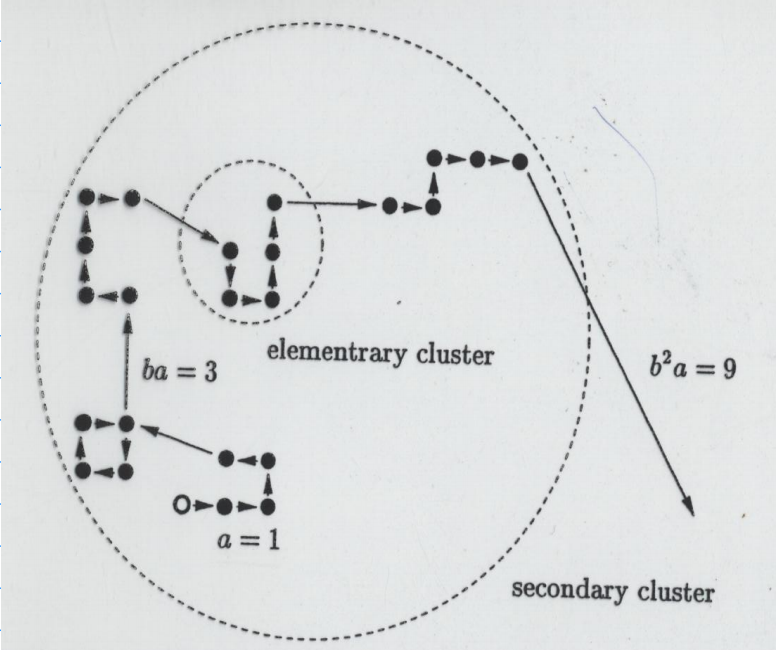
\includegraphics[width=0.4\textwidth]{figures/10_RWWeierstrass.png}
    \caption{\scriptsize Random Walk di Weierstrass ($b=3$, $M=4$): formazione dei Cluster (Paul and Baschangel: Stochastic Process, Springer).}
    \label{fig:figures-10_RWWeierstrass-png}
\end{figure}
\noindent
Proprio per la formazione di questi cluster su scale spaziali diverse il sistema può presentare un comportamento auto-similare.\\
Possiamo notare anche come cambiano i risultati al variare dei parametri $M$ e $b$:
\begin{figure}[H]
    \centering
    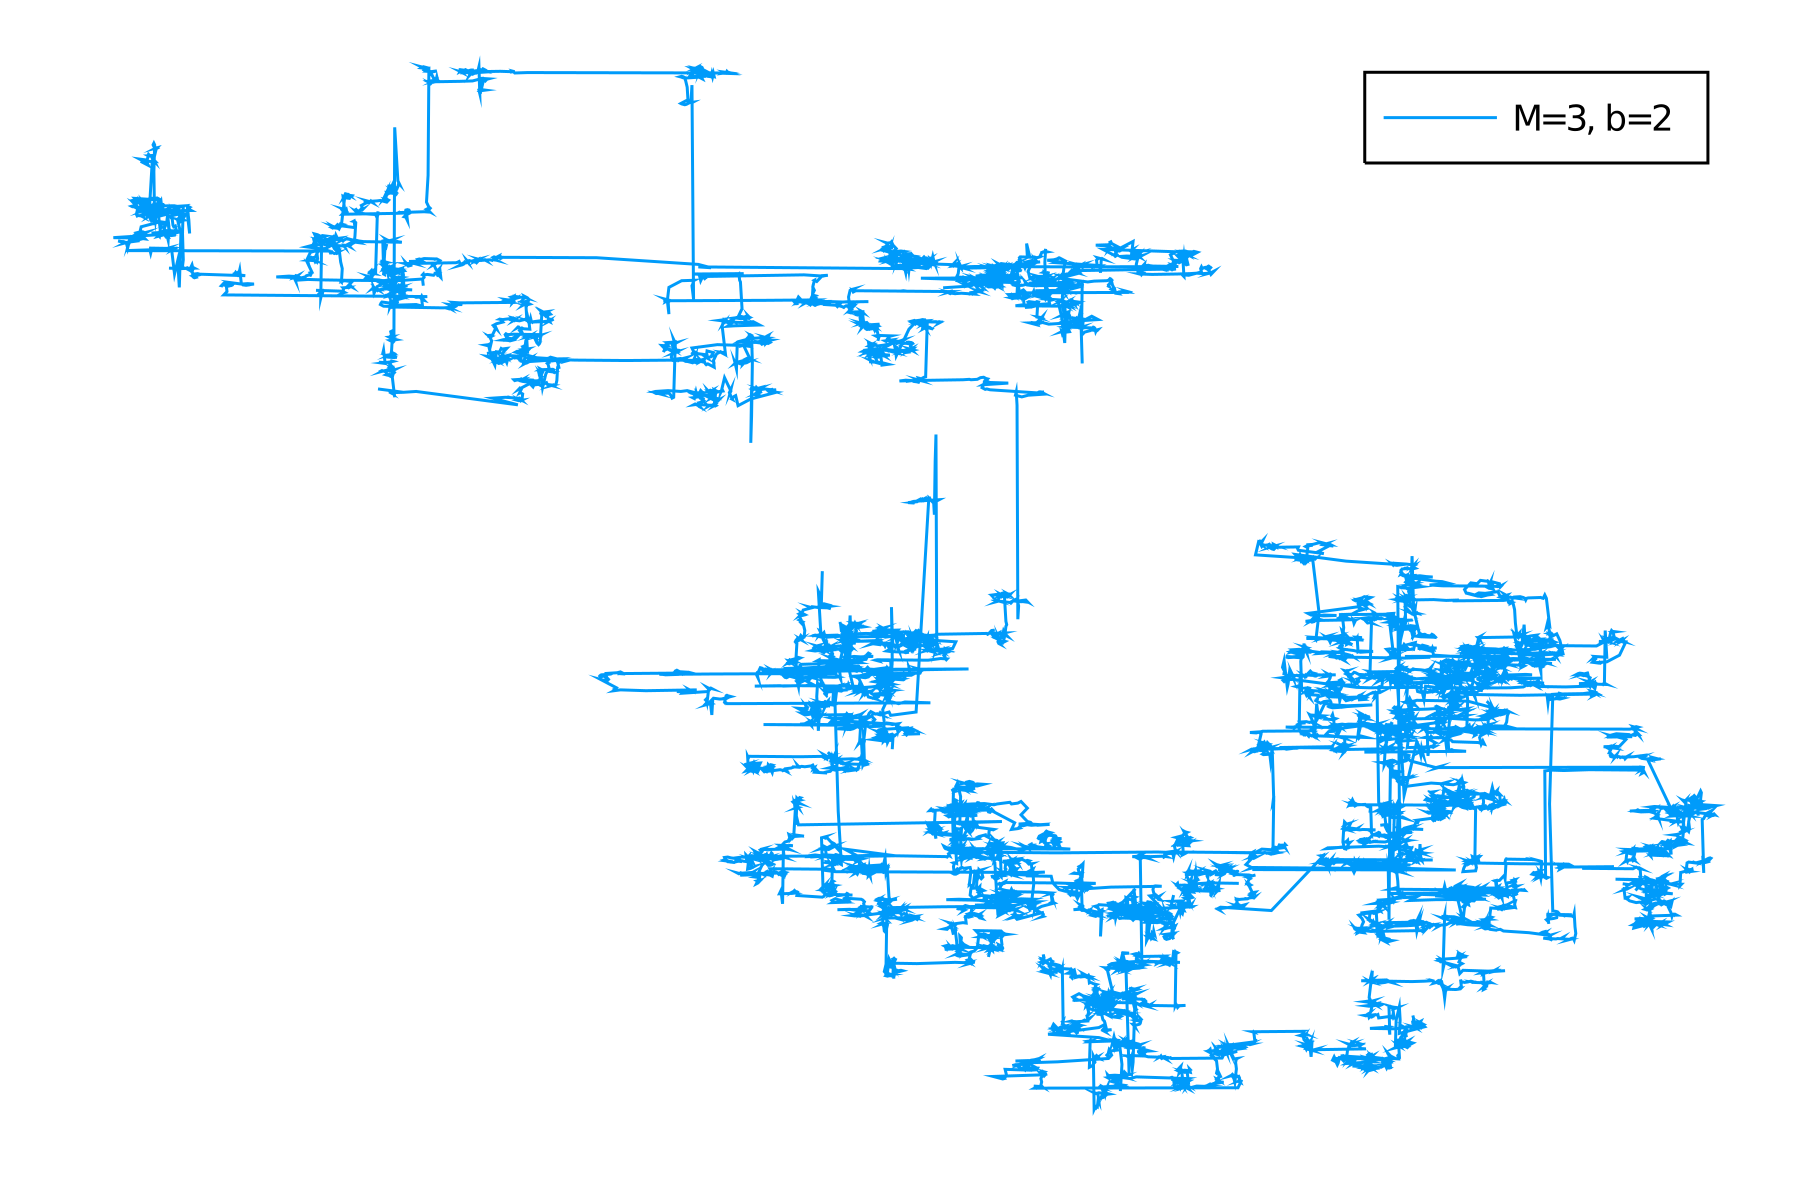
\includegraphics[width=0.45\textwidth]{figures/lez_10_Weier_M_3_b_2.png}
    \caption{\scriptsize Rapporto $M^2 / b = 4.5$.}
    \label{fig:figures-lez_10_Weier_M_3_b_2-png}
\end{figure}
\begin{figure}[H]
    \centering
    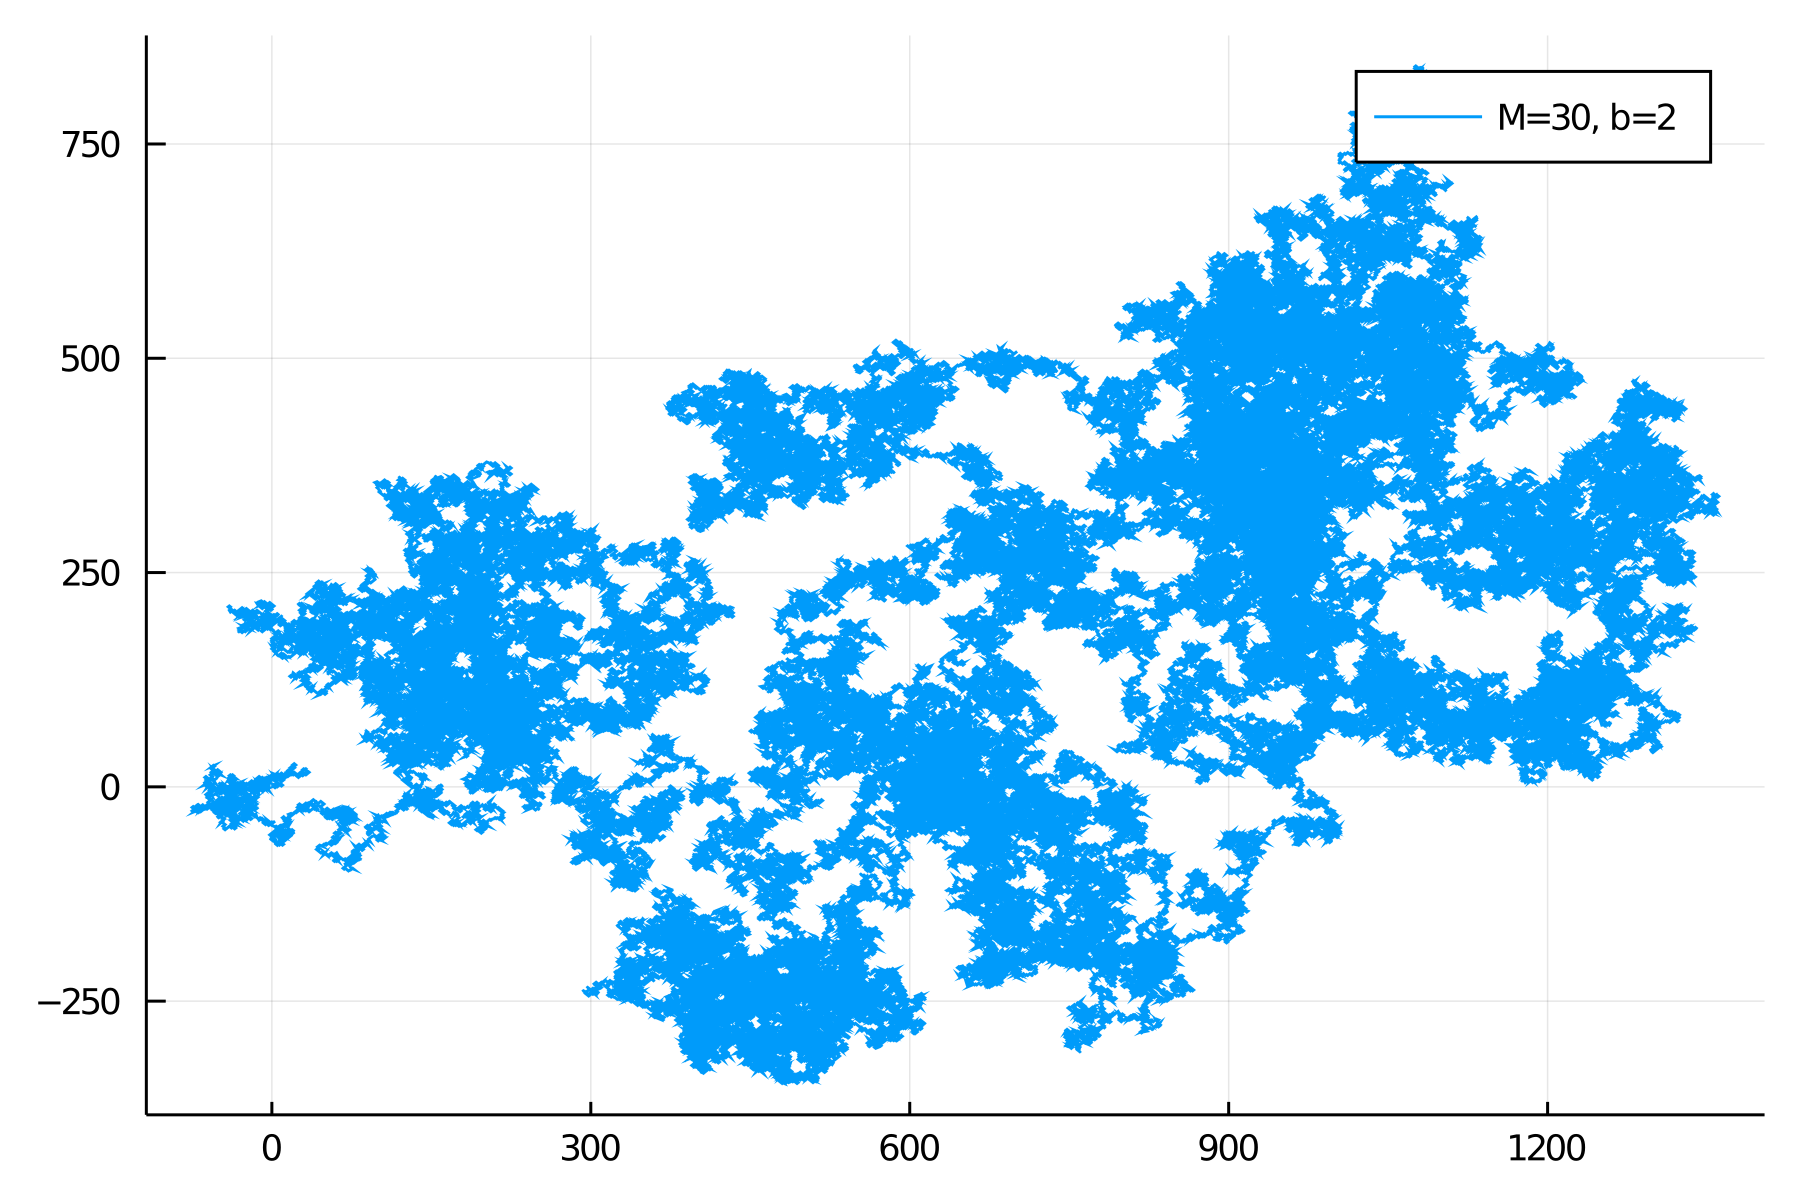
\includegraphics[width=0.45\textwidth]{figures/lez_10_Weier_M_30_b_2.png}
    \caption{\scriptsize Rapporto $M^2 / b = 450$, notiamo come i cluster che si formano siano diversi nei due casi.}
    \label{fig:figures-lez_10_Weier_M_3_b_2-png}
\end{figure}

Risolviamo per $\left<l^2\right>\to 0$, quindi il caso in cui la distribuzione $P(l)$  non può tendere ad una Gaussiana.
\[
    \left<l^2\right> = \frac{\left(M-1\right)a^2}{M}\sum_{}^{} \left(\frac{b^2}{M}\right)^J; \quad \frac{b^2}{M}>1
.\] 


\section{Lezione 11}%
\label{sub:Lezione 11-1}
\section*{Parte 1}%
\label{sub:Parte 1}

\subsection{Equazione di Fokker-Plank: soluzione analitica.}%
\label{sub:Equazione di Fokker-Plank: soluzione analitica.}
Questa lezione è una lunga nota storica su come facevano i nostri antenati a risolvere l'equazione di FK negli anni 80-90 con le mani. L'utilità sta nel fatto che ci da gli strumenti per affrontare la prossima lezione che è invece concettualmente molto interessante.\\
Abbiamo visto nella Lezione \ref{sub:Lezione 4} la forma differenziale di Chapman-Kolmogorov (equazione \ref{eq:4_CK}). La parte di tale equazione che conteneva termini di derivate prime e seconde (quindi quella riguardante la parte continua del processo) è nota come 
\begin{redbox}{Equazione di Fokker-Plank.}
   \[\begin{aligned}
       \partial_{t}P(\vect{x}, t) = &
      				      -\partial_{x_i}A_i(\vect{x}, t) P(\vect{x}, t) + \\
				    & + \frac{1}{2}\partial_{x_i}\partial_{x_J}B_{iJ}(\vect{x},t) P(\vect{x},t) 
   .\end{aligned}\]	 
\end{redbox}
\noindent
In qui il termine $B_{iJ}$ ricordiamo essere il termine di diffusione.\\
Modernamente questa equazione viene risolta numericamente per quasi tutti i casi "interessanti". Tuttavia ci sono alcune situazioni in cui si riesce a risolvere analiticamente, concentriamo questa lezione su quelle.\\
Definiamo una corrente $\vect{J}$:
\[
    J_i = \left(A_i - \frac{1}{2}\partial_{x_J}B_{iJ}\right)P(\vect{x},t) 
.\] 
Quindi l'equazione di FK si scrive come:
\[
    \partial_{t}P + \nabla \vect{J} = 0
.\] 
Quindi possiamo integrare $P$ su un volume $V$ e sfruttare il teorema di Gauss:
\[\begin{aligned}
    \partial_{t}\int\limits_{V} PdV = - \int\limits_{V}  \nabla \vect{J} dV = - \int\limits_{\partial V} d\vect{s}\cdot \vect{J}
.\end{aligned}\]
Dove $\partial V$ è il bordo del volume $V$ (e l'ultima espressione dopo l'uguale è il flusso di $\vect{J}$ sul bordo di $V$). 
\begin{greenbox}{}
    La variazione della probabilità in un volume $V$ è legata al flusso della corrente di probabilità.
\end{greenbox}
\noindent
Quindi la soluzione di questa equazione alle derivate parziali dipende fortemente dall'andamento della corrente lungo la superficie di $V$.
\subsection{Condizioni al bordo per la soluzione della FK.}%
\label{sub:Condizioni al bordo per la soluzione della FK.}
\paragraph{Condizioni al bordo riflettenti.}%
Questo è il caso in cui la corrente di probabilità rispetta la seguente:
\[
    \hat{S}\vect{J} (\vect{z}, t) = 0
.\] 
Con $\hat{S}$ versore del bordo di $V$. Questa condizione implica che la $\vect{J}$ è parallela alla superficie.
\paragraph{Condizioni al bordo assorbenti.}%
\[
    \text{Se }\vect{z}  \in \partial S \implies  J(\vect{z}, t) = 0
.\] 
\paragraph{Condizioni al bordo discontinue}%
La corrente può essere discontinua sul bordo, in queste condizioni il moto resta possibile, la corrente deve soddisfare l'equazione:
\[
    \hat{S}\left(\vect{J} (\vect{z}^+) - \vect{J} (\vect{z}^-) \right) = 0
.\] 
\paragraph{Condizioni al bordo periodiche.}%
Mettiamoci in una dimensione ad esempio, nel segmento $\left[a, b\right]$, allora le condizioni al contorno periodiche implicano che:
\[\begin{aligned}
    & P(a^+) = P(b^-) \\
    & \vect{J} (a^+) = \vect{J} (b^-) 
.\end{aligned}\]
\paragraph{Condizioni al bordo all'infinito.}%
Tipicamente si lavora con oggetti che possono trovarsi a distanze finite, in tal caso le condizioni all'infinito vengono prese come:
\[\begin{aligned}
    & P(\vect{x}, t) \to 0 \quad \left|x\right|\to \infty\\
    & \vect{J} (\vect{x}, t) \to 0 \quad \left|x\right|\to \infty
.\end{aligned}\]
Se così non fosse allora una delle due quantità dovrebbe divergere.
\paragraph{Diffusione nulla al bordo.}%
Se $B_{iJ} = 0$ sul bordo del volume abbiamo una situazione totalmente deterministica. In tal caso tale zona potrebbe essere: 
\begin{itemize}
    \item Un ingresso dei camminatori
    \item Una uscita dei camminatori
\end{itemize}
In questo caso possono esistere delle situazioni ancor più esoteriche in cui oltre che ad avere $B_{iJ} = 0$ sul bordo si ha anche $A(\vect{z}) = 0$. In questo caso speciale i camminatori che raggiungono il bordo si fermano.
\begin{exmp}[]
    \[
        dx = -\alpha xdt + xd\omega
    .\] 
    In questo caso il camminatore che arriva nell'origine si ferma. L'equazione di FK in questo caso può esser scritta riprendendo la formula \ref{eq:8_CK-SDE}:
    \[
        \partial_{t}P = \left[\partial_{x}\alpha x + \frac{1}{2}\partial^2_{x^2} x^2\right] P
    .\] 
\end{exmp}
\noindent
\subsection{Distribuzione di equilibrio del processo}%
\label{sub:Distribuzione di equilibrio del processo}
Riscriviamo la corrente esplicitando la derivata $\partial_{x_J}$:
\begin{equation}
    J_i = \left[A_i-\frac{1}{2}\left(\partial_{x_J}B_{iJ}\right)\right]P - \frac{1}{2} B_{iJ}\partial_{x_J}P
    \label{eq:11_J}
\end{equation}
Cerchiamo una distribuzione di equilibrio con le seguenti ipotesi:
\begin{itemize}
    \item $\vect{J}$ si conserva e all'equilibrio $J=0$ .
    \item All'infinito la distribuzione di probabilità si annulla.
    \item $B_{iJ}$ invertibile.
\end{itemize}
Vogliamo allora capire con queste supposizioni quanto vale $\partial_{x_J}P$.
Si procede invertendo l'espressione \ref{11_J}:
\[
    \partial_{x_J}P = 2B^{-1}_{iJ}\left[A_i-\frac{1}{2}\partial_{x_k}B_{ik}\right]P
.\] 
Quindi portando a sinistra la $P$ si ha anche:
\[
    \frac{\partial }{\partial x_J} \ln (P) = 2B_{iJ}^{-1}\left[A_i-\partial_{x_k}B_{ik}\right]
.\] 
Quindi abbiamo a sinistra un gradiente, come conseguenza anche la quantità a destra deve essere un gradiente.
Per le proprietà del gradiente deve essere vero che:
\[
    \text{rot}(\nabla f)  = 0 \quad \forall f
.\] 
Quindi:
\[
    Z_J\left[A,B, \vect{x}\right] \equiv 2B_{iJ}^{-1}\left[A_i - \partial_{x_k}B_{ik}\right]
.\] 
\begin{equation}
    \text{rot}(Z_J) = 0
    \label{eq:11_rot}
\end{equation}
Di fatto questa condizione si traduce in:
\[
  \frac{\partial }{\partial x_i} Z_J = \frac{\partial }{\partial x_J} Z_i  
.\] 
Se vale questa condizione possiamo allora integrare lungo una curva generica, si ottiene che:
\[
    P_{st}(\vect{x}) = \exp\left(\int\limits^{x} d\vect{s}\vect{Z}\left[A,B, \vect{s}\right]\right)
\] 
In cui si definisce 
\begin{redbox}{Forma potenziale}
    \begin{equation}
	P(\vect{x})  = \exp (-\phi (\vect{x})) 
	\label{eq:11_forma_pot}
    \end{equation}
    con 
     \[
	\phi (\vect{x}) = - \int\limits^{x} d\vect{s}\vect{Z} 
    .\] 
\end{redbox}
\noindent
Tutto questo metodo funziona se si verifica il fatto che $\text{rot}(\vect{Z}) = 0$. Nei casi in cui questa condizione non si avvera non è possibile integrare l'equazione ed ottenere il risultato stazionario \ref{eq:11_forma_pot}.
\begin{exmp}[Processo di Wiener]
    \[
	dx = f(x) dt + Bd\omega
    .\] 
    La FK si scrive come:
    \[
        \partial_{t}P = \left(- \partial_{x}f + \frac{1}{2} B^2\partial^2_{x^2}\right)P; \qquad
	Z = \frac{2f}{B^2}
    .\] 
    Con $Z$  valutato come sopra (tramite la corrente stazionaria). Quindi si ha che:
    \[
	P_{st}\sim \exp\left(\int\limits^{x} \frac{2f}{B^2}dx \right) 
    .\] 
    \begin{greenbox}{}
        I processi di Wiener hanno una distribuzione di equilibrio.
    \end{greenbox}
    \noindent
    Ovviamente è necessario avere una $f$ che si comporti bene asintoticamente (se ho $f=x$ rompo il metodo).
\end{exmp}
\noindent

\begin{exmp}[Processo di OU]
    Prendiamo la stessa equazione dell'esempio precedente
    \[
	dx = f(x) dt + Bd\omega
    .\] 
    tuttavia adesso il termine $Bd\omega$ anziché essere un processo di Wiener (come si sottointende di solito) lo ipotizziamo di Ornstein-Ulhenback:
    \[
	\begin{cases}
	    Bd\omega  = Bydt\\
	    dy = -\dfrac{1}{\tau}ydt + d\omega
	\end{cases}
    \] 
    Dove il $d\omega$ nel sistema è adesso un processo di Wiener.\\
    Ricordiamo che questo processo è caratterizzato da avere un taglio in frequenza di $\frac{1}{\tau}$.\\
    Per semplificare ancora i conti inseriamo all'interno della SDE un secondo processo di Wiener $d\omega_2$ (si capirà meglio sotto), si ottiene allora il sistema:
    \[
        \begin{cases}
	    dx = \left(f(x) + By\right)dt + d\omega_2\\
	    dy = -\dfrac{1}{\tau}y dt + d\omega_1
        \end{cases}
    .\] 
    In questo caso è evidente che i termini della FK in due dimensioni
    \footnote{Si tratta di due dimensioni perché abbiamo una coppia di variabili stocastiche: $x$ e $y$.}
     corrispondono alle quantità:
    \[\begin{aligned}
	&A_x = f+By & \quad B_{xx} = 1\\
	&A_y = -\frac{1}{\tau}y &\quad B_{yy}=1
    .\end{aligned}\]
    Possiamo scrivere la matrice del rumore $B$ considerando i coefficienti a moltiplicare i due processi di Wiener $d\omega_1, d\omega_2$ nelle equazioni. Visto che i due processi sono indipendenti e compaiono uno per l'equazione di $x$ e l'altro per l'equazione di $y$ si ha:
    \[
        B = 
	\begin{pmatrix}
	    B_{xx} & B_{xy}\\
	    B_{yx} & B_{yy}
	\end{pmatrix}
	=
	\begin{pmatrix}
	    1 & 0\\
	    0 & 1
        \end{pmatrix}
    .\] 
    In conclusione possiamo scrivere l'equazione di FK:
    \[\begin{aligned}
	\partial_{t}P(x,y) = \left[-\partial_{x}A_x - \partial_{y}A_y + \frac{1}{2}(\partial^2_{x^2}+\partial^2_{y^2}) \right]P(x,y) 
    .\end{aligned}\]
    Possiamo allora calcolare $Z_x$ e $Z_y$ ($B$ è l'identità quindi $B^{-1} = B$):
    \[
	 Z_x = 2(f+By) \qquad
	 Z_y = -\frac{2y}{\tau}
    .\] 
    Per essere una divergenza $\vect{Z}$ deve rispettare la condizione del rotore:
    \[
	\text{rot}(\vect{Z}) = 0
    .\] 
    Tuttavia questa condizione non è soddisfatta:
    \[
        \partial_{y}Z_x = 2B \neq \partial_{x}Z_y = 0
    .\] 
    Quindi questo processo non soddisfa la condizione di potenziale.
    \begin{greenbox}{}
        I processi di Ornstein-Ulhenback non hanno una distribuzione di equilibrio.
    \end{greenbox}
    \noindent
    Questo non significa che integrando questa equazione numericamente non si possa ottenere niente, questo tipo di processi presenta una \textbf{distribuzione di quasi equilibrio} (approfondiremo più avanti).
\end{exmp}
\noindent
\begin{exmp}[OU modificato]
Prendiamo lo stesso moto analizzato nell'esempio precedente ed aggiungiamo il termine $Bxdt$ all'equazione per $y$:
    \[
        \begin{cases}
	    dx = \left(f(x) + By\right)dt + d\omega_2\\
	    dy = -\dfrac{1}{\tau} y dt + Bxdt + d\omega_1
        \end{cases}
    .\] 
In questo caso abbiamo che:
\[\begin{aligned}
	&A_x = f+By & \quad B_{xx} = 1\\
	&A_y = -\frac{1}{\tau}y + Bx &\quad B_{yy}=1
.\end{aligned}\]
Mentre la matrice $B$ non cambia:
    \[
        B = 
	\begin{pmatrix}
	    B_{xx} & B_{xy}\\
	    B_{yx} & B_{yy}
	\end{pmatrix}
	=
	\begin{pmatrix}
	    1 & 0\\
	    0 & 1
        \end{pmatrix}
    .\] 
    Ed anche l'equazione di FP resta della stessa forma:
    \[\begin{aligned}
	\partial_{t}P(x,y) = \left[-\partial_{x}A_x - \partial_{y}A_y + \frac{1}{2}(\partial^2_{x^2}+\partial^2_{y^2}) \right]P(x,y) 
    .\end{aligned}\]
    Quello che cambia è la forma di $A_y$, che contiene il termine $Bx$ in più rispetto a prima. Questo comporta anche dei valori delle componenti di $\vect{Z}$ diversi:
    \[
	Z_x = 2(f+By) \qquad Z_y = -\frac{2y}{\tau}+2Bx
    .\] 
    Il rotore di $\vect{Z}$ è nullo grazie al termine aggiuntivo.\\
    Il termine aggiunto è quindi un termine ad-hoc per rendere il metodo visto sopra applicabile, infatti in questo modo è possibile avere una soluzione potenziale.
    \[
        P_{st}\sim \exp(\phi )
    .\] 
    con 
    \[\begin{aligned}
	\phi =& - \int\limits^{\vect{x}} d\vect{s}\vect{Z}  = \\
	      &= - \int\limits^{\vect{x}} (f+By)dx + \left(-\frac{y}{\tau} + Bx\right)dy = \\
	      &= \left(-\int\limits^{\vect{x}} fdx \right)-Bxy + \frac{y^2}{2\tau}
    .\end{aligned}\]
    Ricordiamo che gli integrali con pedice $\vect{x}$ sono integrali di linea, sul percorso $\vect{x}$ ad intervalli $d\vect{s}$.\\
    Questa cosa ha anche un senso fisico, infatti le equazioni differenziali per $x$ e $y$ possono essere riscritte come:
    \[\begin{aligned}
	&\frac{\text{d} x}{\text{d} t} = - \partial_{x}\left(-\int\limits^{\vect{x}} fdx - Bxy + \frac{y^2}{2\tau}\right) + \xi_x\\
	&\frac{\text{d} y}{\text{d} t} = - \partial_{y}\left(-\int\limits^{\vect{x}} fdx - Bxy + \frac{y^2}{2\tau}\right) + \xi_y
    .\end{aligned}\]
    Poiché svolgendo le derivate alcuni termini si annullano e tornano le due equazioni sopra ($xi = d\omega /dt$).\\
    Quindi le due equazioni si presentano in termini di equazioni del moto classiche, nella quale il termine che viene derivato rispetto alla coordinata in ciascuna equazione funge da potenziale.
\end{exmp}
\noindent
\subsection{Bilancio dettagliato}%
\label{sub:Bilancio dettagliato}
Il principio del bilancio dettagliato detta la struttura della equazione di FP e permetterà di risolverla in certe condizioni.\\
Il fatto che la corrente sia nulla e che si possa costruire un potenziale equivale a dire che il sistema presenta il bilancio dettagliato.
\subsubsection{Sistema di particelle in moto}%
\label{subsub:Sistema di particelle in moto}
Supponiamo di avere un sistema di oggetti caratterizzati da una posizione ed una  velocità ad un certo istante $(r,v,t)$.
La probabilità di trovarsi in $(r,v,t)$ e ad un altro istante in $(r',v',t')$ può essere scritta come probabilità congiunta:
\[
    P(r',v',t+\tau; r,v,t) \qquad t' = t+\tau
.\] 
Per trovare questa quantità possiamo ragionare in termini di propagatore (come abbiamo fatto nelle lezioni precedenti).
\[
    (r,v,t) \to (r',v',t+\tau) 
.\] 
\subsubsection{Metodo "Nolandiano"}%
\label{subsub:Metodo "Nolandiano"}
Possiamo chiederci quale sia la probabilità del processo inverso.
\[
    (r',v',t+\tau) \to (r,v,t') 
.\] 
Anziché pensare ad una inversione temporale per risalire ad un istante precedente possiamo decidere di invertire puntualmente la velocità. In questo modo manteniamo l'ordine temporale mentre gli oggetti si muovono all'indietro (vedi Tenet)
\[
    (r',-v',t) \to (r,-v,t+\tau) 
.\] 
\begin{redbox}{Conseguenza del Bilancio dettagliato}
    Se il sistema presenta bilancio dettagliato allora vale che:
    \[
    P(r',v',t+\tau; r,v,t) = P(r,-v,t+\tau; r',-v',t)
    .\] 
\end{redbox}
\noindent
Ovviamente in un caso stazionario avviamo anche l'invarianza per traslazione temporale, quindi possiamo considerare l'istante $t=0$:
\[
    P_s(r',v',\tau; r,v,0) = P_s(r,-v,\tau; r',-v',0)
.\] 
Ipotizziamo adesso che il processo sia Markoviano. In tal caso la probabilità composta si può esprimere in termini della distribuzione stazionaria $P_s(r,v)$ e del propagatore:
\[\begin{aligned}
    P&(r',v',\tau|r,v,0) P_s(r,v) =\\
     & =P(r,-v,\tau|r',-v',0) P_s(r',-v')
.\end{aligned}\]
Possiamo manipolare questa espressione valutando quali variabili cambiano segno sotto inversione temporale, in generale è vero che:
\begin{itemize}
    \item Le variabili di tipo "coordinate" non cambiano segno
	\[
	    t\to -t \implies  x \to x
	.\] 
    \item Le variabili di tipo velocità cambiano segno
	\[
	    t\to -t \implies  v_x \to -v_x
	.\] 
\end{itemize}
Prendendo delle coordinate generalizzate $x_i$ abbiamo che per inversione temporale:
\[
    x_i \xrightarrow[]{t\to -t} \epsilon_i x_i \qquad \epsilon_i = \pm 1
.\] 
Quindi ragionando in termini vettoriali:
\[
    \vect{x}  = (x,y,z,v_x,v_y,v_z) 
.\] 
La notazione usata allude alle coordinate di una singola particella, si può generalizzare una vettore $\vect{x}$ a $n$ particelle mettendo tutte le coordinate delle particelle $1,\ldots,n$ all'interno del vettore.\\
Possiamo riscrivere in modo generale i passaggi precedenti\footnote{Si è invertita la notazione degli indici primati\ldots}
:
\[
    P(\vect{x}, t+\tau ; \vect{x}', t) = 
    P(\vect{\epsilon}\cdot \vect{x}', t+\tau ; \vect{\epsilon}\cdot \vect{x}, t) 
.\] 
Prendiamo le condizioni "iniziali" per $\tau=0$:
\[\begin{aligned}
    \tau & = 0 :\\
	     &\implies  \delta (\vect{x}-\vect{x}') P_s(\vect{x}') = \delta (\vect{\epsilon} (\vect{x}'-\vect{x})) P_s(\vect{\epsilon}\vect{x}) 
.\end{aligned}\]
Sfruttando il fatto che la $\delta$ è pari e che la $\delta$ di una quantità vettoriale può essere vista come il prodotto di $\delta$ se ne conclude che:
\begin{redbox}{}
    \[\begin{aligned}
	P_s(\vect{x}') &= P_s(\vect{\epsilon}\cdot \vect{x}) \\
		       & \Downarrow\\
	P(\vect{x},t|\vect{x}', 0) P_s(\vect{x}') &=
        P\left(\vect{\epsilon}\vect{x}',\tau|\vect{\epsilon}\vect{x},0\right)P_s(\vect{x}') 
    .\end{aligned}\]
\end{redbox}
\noindent
La prima comporta che $P_s$ dovrà essere una potenza pari delle $v$ poiché queste ultime cambiano di segno quando si applica $\epsilon$.
\subsubsection{Conseguenze del bilancio dettagliato applicato ad una Chapman-Kolmogorov}%
\label{subsub:Conseguenze del bilancio dettagliato applicato ad una Chapman-Kolmogorov}
Si può dimostrare che (libro di Van Kampen) il bilancio dettagliato permette di descrivere la struttura generale dei vari termini della equazione di CK (equazione \ref{eq:4_CK}), le seguenti formule sono pura referenza ma ne faremo uso\ldots
\begin{equation} 
\begin{aligned}
    &\omega (\vect{x}|\vect{x}') P_s(\vect{x}') = \omega (\vect{\epsilon} \vect{x}'|\vect{\epsilon} \vect{x}) P_s(\vect{x}) \\
    &\epsilon_i A_i(\vect{\epsilon}\vect{x}) P_s(\vect{x}) =\left[-A_i(\vect{x}) + \frac{\partial }{\partial x_J} B_{iJ}(\vect{x})\right]P_s(\vect{x}) \\
    & \epsilon_i \epsilon_J B_{iJ}(\epsilon x) = B_{iJ}(\vect{x}) 
    \label{eq:11_ref}
.\end{aligned}\end{equation}
\subsubsection{Nota storica sul Bilancio dettagliato}%
\label{subsub:Nota storica sul Bilancio dettagliato}
Storicamente si sono introdotte due quantità per capire se il sistema presenta il bilancio dettagliato:
\[\begin{aligned}
    & D^{\text{irr}}_i = \frac{1}{2}\left(A_i(x) + \epsilon_i A_i(\epsilon_ix)\right)\\
    & D^{\text{rev}}_i = \frac{1}{2}\left(A_i(x) - \epsilon_iA_i(\epsilon_ix) \right)
.\end{aligned}\]
Infatti se la $D^{\text{irr}}_i\neq 0$ allora il sistema non presenta il bilancio dettagliato.

\begin{exmp}[]
    \[
        \begin{cases}
            dx = vdt\\
	    mdv = -V'(x) dt - \gamma v dt + \sqrt{2\gamma  k_B T} d\omega
        \end{cases}
    .\] 
    In cui si ha un termine di attrito alla Stokes:
    \[
        \gamma = 6\pi  \eta r
    .\] 
   L'equazione di FK che ne emerge è la seguente:
   \[\begin{aligned}
       &\partial_{t}P =\\
       &=-\partial_{x}v + \frac{1}{m}\partial_{v}\left[\left(V'(x) + \gamma v\right)P\right] + 
		      +\frac{\gamma k_b T}{m^2}\partial^2_{v^2}P
   .\end{aligned}\]
   Quindi abbiamo che:
   \[
       A = \begin{pmatrix} v \\ - \frac{\gamma  v}{m} - \frac{V'}{m}\end{pmatrix} 
       \qquad 
       B = \begin{pmatrix} 
	   0 & 0 \\
	   0 & \frac{2\gamma k_BT}{m^2}
           \end{pmatrix} 
   .\] 
   Visto che il termine di inversione $\vect{\epsilon}$ ci da:
   \[
       \vect{\epsilon}\cdot \begin{pmatrix} x \\ v \end{pmatrix} = \begin{pmatrix} x \\ -v \end{pmatrix} 
   .\] 
   Si ha anche che (si applica $\epsilon$ due volte, quindi dove opportuno c'è un doppio cambio di segno):
   \[
       \vect{\epsilon}\vect{ A}(\vect{\epsilon}\vect{x})   = \begin{pmatrix} -v \\ -\frac{\gamma v}{m} + \frac{V'}{m} \end{pmatrix} 
   .\] 
   Applicando adesso la seconda delle \ref{eq:11_ref}:
   \[\begin{aligned}
       \epsilon A(\epsilon x) P_s(x) &= - A(x) P_(x) + \partial_{J}B_{iJ}P_s(x) \\
				   & \Downarrow\\
       \begin{pmatrix} -v \\ -\frac{\gamma v}{m} + \frac{V'}{m} \end{pmatrix} P_s &= 
       \begin{pmatrix} -v \\ \frac{\gamma v}{m}+\frac{V'}{m} \end{pmatrix} P_s + 
       \begin{pmatrix} 0 \\ \partial_{v}\left(\frac{2\gamma k_BT}{m^2}\right) \end{pmatrix} P_s
   .\end{aligned}\]
   Notiamo che la derivata $J$ in questo caso indica la derivata sulla seconda componente: la velocità.\\
   La prima riga è una identità, la seconda riga invece è meno ovvia:
   \[
       -\frac{2\gamma v}{m}P_s = \frac{2\gamma k_BT}{m^2}\partial_{v}P_s
   .\] 
   Se risolviamo si ha una forma per la $P_s(x, v)$:
   \[
       P_s(x,v) = \exp\left(-\frac{v^2m}{2k_BT}\right)f(x) 
   .\] 
   Notiamo come la distribuzione stazionaria $P_s(x,v) $ sia quadratica in $v$.
   Questo, a conferma di quanto accennato prima, è dovuto all'invarianza di tale distribuzione quando si applica $\vect{\epsilon }$. \\
   Per trovare la $f(x) $ basta reinserire la $P_s$ nella equazione di FK,  si impone che il processo sia stazionario ($\partial_{t}P_s = 0$) e si ottiene:
   \[\begin{aligned}
       v\partial_{x}f(x) &= - \frac{v}{k_BT}V'(x) f(x) \\
			 &\Downarrow\\
       f(x) &\propto \exp\left(-\frac{V(x)}{k_BT}\right)
   .\end{aligned}\]
   In conclusione la distribuzione di equilibrio è la seguente:
   \[
       P_{s} = N \exp\left(-\frac{1}{k_BT}\left(\frac{mv^2}{2}+V(x)\right)\right)
   .\] 
   Notiamo come la forma sia esattamente quella che ci si aspetta da un caso fisico:
   \[
       P\sim \exp\left(-\beta H\right)
   .\] 
\end{exmp}
\noindent
Nell'esempio precedente si è legato il termine di dissipazione al termine stocastico (nelle SDE) nella formula:
\[
	    mdv = -V'(x) dt - \gamma v dt + \sqrt{2\gamma  k_B T} d\omega
.\] 
Notiamo infatti che $\gamma$ compare sia nel termine per $dt$ che in quello per $d\omega$.\\
Il motivo per il quale lo abbiamo fatto è dovuto ad un importante teorema.
\subsection{Relazione di Onsager e Teorema di Fluttuazione Dissipazione.}%
\label{sub:Relazione di Onsager e Teorema di Fluttuazione Dissipazione.}
Prendiamo un processo di OU nel quale all'interno della FK il termine $A$ è lineare ed il termine $B$ è costante
\[
    A_i(x) = A_{iJ}x_J \qquad
    B_{iJ}(x) = B_{iJ}
.\] 
Questa linearizzazione valuta le piccole oscillazioni attorno al punto di equilibrio per un processo di OU.\\
Se un processo ha le seguenti proprietà sotto inversione temporale
\footnote{Riscrivo le \ref{eq:11_ref} in un'altra forma, esplicitando il fatto che $B_{iJ}$ è costante.}
:
\begin{equation}
\begin{aligned}
    &\epsilon_i\epsilon_J B_{iJ}=B_{iJ}\\
    &\left(\epsilon_i\epsilon_JA_{iJ} + A_{iJ}\right)x_J = B_{iJ}\partial_{J}\ln P_s \label{eq:11_B}
\end{aligned}
\end{equation}
Allora è sempre vero che:
\[
    P_s = N \exp\left(-\frac{1}{2}x^tD^{-1}x\right)
.\] 
Con $D^{-1}$ simmetrica.\\
Se vale il principio del bilancio dettagliato allora esistono delle relazioni che legano la matrice $D^{-1}$ (che contiene l'equivalente della temperatura del sistema) ai vettori $A$:
\begin{equation}
\begin{aligned}
    &\epsilon A\epsilon  = D A^tD^{-1} \\
    &\epsilon A\epsilon D = D A^t \\
    &\epsilon (AD) = (AD)^t\epsilon\\
    & B = -\left(AD + DA^t\right) \label{eq:11_B1}
.\end{aligned}
\end{equation}
Per arrivare a queste conclusioni si è saltata una paccata di algebra noiosa.
\begin{exmp}[Circuito RLC]
    Prendiamo il seguente circuito
    %\begin{center}
\begin{circuitikz}[american, scale = 1.5][americanvoltages]
    \draw (0,0)
    to[] (0,2) 
    to[L, v^<=$L$] (1.5,2) %Inductor One  
    to[R, v^<=$R$] (3,2) % The resistor
    to[C, v^<=$C$] (3,0) %Capacitor Two
    to[V=$V \sim V_0 + \xi$] (0,0); % The voltage source
    \draw[thin, <-, >=triangle 45] (1.5,1)node{$i$}  ++(-60:0.5) arc (-60:170:0.5);
\end{circuitikz}
\end{center}

    Dove la sorgente di potenziale è una soluzione ionica (presenta delle fluttuazioni $\xi$).\\
    L'equazione che determina la corrente nel circuito è:
    \[
        \frac{\text{d} i}{\text{d} t} = \frac{1}{L}\left(-\frac{Q}{C}-iR +V_\xi\right)
    .\] 
    Supponendo che anche la carica sul condensatore senta delle fluttuazioni si ha che:
    \[
	\frac{\text{d} Q}{\text{d} t} = i - \gamma Q + Q_\xi(t) 
    .\] 
    Possiamo scrivere le SDE del processo stocastico come:
    \[
       \begin{cases}
 	 di = - \dfrac{Q}{LC}dt -\dfrac{R}{L}idt +\dfrac{V_\xi}{L}dt\\
	 dQ = idt - \gamma Q dt + Q_\xi dt          
       \end{cases} 
    .\] 
    La matrice $A$ si esprime come:
    \[
        A = 
	\begin{pmatrix} 
	    -\frac{R}{L} & -\frac{1}{LC}\\
	    1            & - \gamma
	\end{pmatrix} 
    .\] 
    Mi aspetto che la distribuzione stazionaria abbia una forma del tipo:
    \[
        P_s \sim \exp\left(-\frac{H}{k_BT}\right)
    .\] 
    L'energia del sistema sappiamo che vale:
    \[
        E = \frac{Li^2}{2} + \frac{Q^2}{2C}
    .\] 
    Guardando i termini dell'energia $\sim H$ ci aspettiamo una matrice $D$ della seguente forma
    \footnote{Dobbiamo considerare che l'inversa entrerà nella espressione per $P_s$}
    :
    \[
        D = 
	\begin{pmatrix}
	    \frac{k_BT}{L} & 0 \\
	    0              & k_BT C
	\end{pmatrix} 
    .\] 
    Mentre per quanto riguarda la matrice di inversione basta considerare l'analogia $(x,v) \to (Q,i)$:
    \[
	\epsilon  = \text{diag}(-1,1) 
    .\] 
    Possiamo verificare che siano rispettate le relazioni sulle matrici $A$ e $D$:
    \[
	AD = 
	\begin{pmatrix} 
	    \dfrac{Rk_BT}{L^2} & &  \dfrac{k_BT}{L}   \\
	     &&\\
	    - \dfrac{k_BT}{L} & & \gamma k_BTC 
	\end{pmatrix} 
    .\] 
    \[
	(AD)_{12} = -(DA)_{21} 
    .\] 
    Inoltre troviamo la matrice $B$ sfruttando l'ultima delle equazioni \ref{eq:11_B1}:
    \[
        B = -\left(AD+DA^t\right) = 2k_BT 
	\begin{pmatrix} 
	    R/L^2 & 0\\
	    0    & \gamma C
	\end{pmatrix} 
    .\] 
    Troviamo allora che tutto il meccanismo delle equazioni esposte sopra funziona in questo esempio.\\
    Quello che cerchiamo adesso è la relazione tra i termini stocastici nelle equazioni ($V_\xi$ e $Q_\xi$) e la temperatura. \\
    Si nota intanto che i due processi stocastici potrebbero essere legati tra loro, ipotizziamo che le variabili stocastiche che descrivono $V_\xi$ e $Q_\xi$ siano $\xi_1$ e $\xi_2$ tali che:
    \[
        \begin{cases}
            V_\xi /L \sim  b_{11} \xi_1 + b_{12}\xi_2\\
	    Q_\xi \sim b_{21}\xi_1 + b_{22}\xi_2
        \end{cases}
    .\] 
    Per avere tutte le formule di equilibrio che abbiamo ottenuto in precedenza la struttura della matrice $b$ deve essere (non ben spiegato perché): 
    \[
        b = 
	\begin{pmatrix} 
	    \sqrt{2k_BTR /L^2} & 0 \\
	    0             & \sqrt{2k_BT\gamma C} 
	\end{pmatrix} 
    .\] 
    Se ricordiamo bene le equazioni di partenza avevano le proprietà:
    \[
        \begin{cases}
            di \sim -\dfrac{R}{L}idt \\
	    dQ \sim - \gamma Qdt
        \end{cases}
    .\] 
    I due termini a moltiplicare $i$ e $Q$ sono proprio i termini che ritroviamo in $b_{11}$ e $b_{22}$.
\end{exmp}
\noindent
\begin{redbox}{Sunto del teorema Flutt. Diss.}
    Dato un processo con 
    \begin{itemize}
        \item Un termine di dissipazione $\gamma$
	\item Un processo stocastico $\xi$.
    \end{itemize}
    Allora l'intensità del processo stocastico vale $\sim \sqrt{2k_BT \gamma}$ (con normalizzazioni opportune)
\end{redbox}
\noindent
\subsection{Fokker-Plank dipendente dal tempo}%
\label{sub:Fokker-Plank dipendente dal tempo}
L'argomento di questa sezione è un pò fumoso, operativamente si capirà meglio il significato con degli esempi pratici\ldots\\
Riprendiamo l'equazione FK e cerchiamo una soluzione non stazionaria.
\begin{equation}
    \partial_{t}P = \left(-\partial_{x}A + \frac{1}{2}\partial^2_{x^2} B\right)P 
    \label{eq:11_FK_t}
\end{equation}
Possiamo vedere il termine nella parentesi di destra come un operatore: $\mathcal{L}$.
\[
    \partial_{t}P = \mathcal{L}P
.\] 
Possiamo vedere questa come una equazione agli autovalori, in tal caso possiamo scrivere la $P$ come una sovrapposizione lineare di autovalori ed autovettori:
\[
    P = P_\lambda (x) e^{-\lambda t}
.\] 
Per poi sostituire nella equazione \ref{eq:11_FK_t} per trovare le soluzioni $P_\lambda, \lambda$:
\begin{equation}
    -\lambda P_\lambda  e^{-\lambda t} = \mathcal{L}P_\lambda  e^{-\lambda t}
    \label{eq:11_FK_auto}
\end{equation}
Possiamo utilizzare la notazione della meccanica quantistica pensando ai $P_\lambda$ nella equazione \ref{eq:11_FK_auto} come dei "ket". \\
Dobbiamo notare che l'equazione che agisce sui ket è nota, mentre quella che agisce sui bra no. Questo perché, a differenza del caso quantistico, qui c'è di mezzo la distribuzione stazionaria. \\
Quindi quando si cerca di applicare l'operatore $\mathcal{L}$ a sinistra si deve tener di conto che va ad agire anche sulla distribuzione stazionaria.\\
Dobbiamo quindi scrivere la $P(x,t)$ come:
\[
    P(x,t) = P_s(x) q(x,t) 
.\] 
Possiamo reinserire questa nella FK dipendente dal tempo e isolare i termini con $P_s$  tramite integrazione par parti. Ne emerge una equazione per $q(x,t)$, che rappresentano i bra, del tipo:
\begin{redbox}{Backward FK}
\[
    \partial_{t}q = A\partial_{x}q + \frac{1}{2}B\partial^2_{x^2}q
.\]     
\end{redbox}
\noindent
Che differisce dalla equazione per il ket dal solo segno del primo termine dopo l'uguale. \\
Abbiamo quindi il set di equazioni agli autovalori:
\begin{equation}
    \begin{cases}
	-\partial_{x}(AP_\lambda) + \dfrac{1}{2}\partial^2_{x^2}(BP_\lambda) = -\lambda P_\lambda\\
	\\
	A\partial_{x}Q_{\lambda'} + \dfrac{1}{2}B\partial^2_{x^2}Q_{\lambda'} = - \lambda'Q_{\lambda'}
    \end{cases}
\end{equation}
A questo punto si tratta di fare fare algebra sulle espressioni, possiamo moltiplicare la prima per $Q_{\lambda'}$, integrarla su un certo intervallo $(a,b)$  ed applicare l'integrazione per parti.\\
Il risultato al quale si arriva è il seguente:
\[\begin{aligned}
    (\lambda'&-\lambda) \int_{a}^{b} Q_{\lambda'}P_{\lambda}dx = \\
             &= \left\{Q_{\lambda'}\left[-AP_\lambda  + \frac{1}{2}\partial_{x}(BP_\lambda) \right] -
		       \frac{1}{2}BP_{\lambda}\partial_{x}Q_{\lambda'}\right\}_{a}^{b}
.\end{aligned}\]
Notiamo ancora l'importanza delle condizioni al contorno su $(a,b)$. 
\begin{exmp}[Condizioni al contorno assorbenti]
    In tal caso il lato destro della equazione si annulla in quanto:
    \[
	Q_{\lambda'}(a) = Q_{\lambda'}(b) = 0
    .\] 
    Quindi il sistema è "bi-ortogonale":
    \[
        \int Q_{\lambda'}P_{\lambda}dx = \delta_{\lambda\lambda'}
    .\] 
\end{exmp}
\noindent
\begin{exmp}[Processo di Wiener con condizioni al bordo ($0,1$) assorbenti.]
    Per via delle condizioni assorbenti in $0$ e $1$ abbiamo che:
    \[
	P(0,t) = P(1,t) = 0
    .\] 
    La FK che descrive il processo di Wiener è:
    \[
        \partial_{t}P = \frac{1}{2}\partial^2_{x^2}P
    .\] 
    Possiamo scegliere la base più semplice per lo sviluppo nell'intervallo che rispetti le condizioni al bordo:
    \[
	P_\lambda =\sin (\pi n x) 
    .\] 
    Quindi ogni $P$ si scrive come sovrapposizione:
    \[
	P(x,t) = \sum_{n=1}^{} b_n e^{-\lambda n t}\sin (\pi n x) 
    .\] 
    Inserendo nell'equazione per $P$  si ottengono gli autovalori:
    \[
        \lambda_n = \frac{n^2\pi^2}{2}
    .\] 
    Per quanto riguarda i coefficienti $b_n$  dobbiamo imporre delle condizioni iniziali:
    \[
	P(x,0) = \delta (x-x_0) 
    .\] 
    Quindi
    \[
	b_n = b_n(0) = \int_{0}^{1} \delta (x-x_0) \sin (n\pi x)  dx = \sin (n\pi x_0) 
    .\] 
    E con questo il problema è risolto, infatti si ha:
    \[
	P(x,t|x_0, 0) = \sum_{n=1}^{\infty} \sin (\pi nx_0) \sin (n\pi x) \exp\left(-\frac{n^2\pi^2 }{2}t\right)
    .\] 
\end{exmp}
\noindent
\begin{exmp}[Processo di Wiener in $(0,1)$ con condizioni riflettenti]
    Le condizioni riflettenti al bordo implicano che la corrente $J$ si annulla al bordo, vista l'espressione di $J$ (e ricordando che $A=0$ per il processo di Wiener) si ha:
    \[
	\frac{\partial P(0,t) }{\partial x} = \frac{\partial P(1,t) }{\partial x} = 0
    .\] 
    Quindi una base opportuna per le soluzioni è quella del coseno. Otteniamo quindi gli stessi autovalori del caso precedente:
    \[
        \lambda_n = \frac{n^2\pi^2}{2}
    .\] 
    Ma le autofunzioni sono adesso dei coseni, la soluzione finale è:
    \[
	P(x,t|x_0, 0) = \sum_{n=-\infty}^{\infty} \cos (\pi nx_0) \cos (n\pi x) \exp\left(-\frac{n^2\pi^2 }{2}t\right)
    .\] 
\end{exmp}
\noindent
\clearpage

\section*{Parte 2}%
\label{sub:Parte 2}
\subsection{Tempo di primo passaggio o MFPT}%
\label{sub:Tempo di primo passaggio o MFPT}
Ipotizziamo di avere un fenomeno stocastico e di osservarne l'andamento temporale. Possiamo ipotizzare anche che questo fenomeno presenti dei picchi randomici in maniera irregolare. \\
In questa lezione cerchiamo un metodo analitico per esprimere l'intervallo temporale medio tra due eventi di questo tipo, anche detto tempo di primo passaggio.\\
Operativamente dobbiamo:
\begin{itemize}
    \item Creare un modello del fenomeno in termini stocastici.
    \item Derivare una qualche quantità dal modello che ci permetta di calcolare il tempo medio tra gli eventi.
\end{itemize}
Ad esempio possiamo avere una certa distribuzione iniziale di oggetti (o camminatori):
%\tikzmath{\s = 1;}
\begin{figure}[H]
    \centering
    \begin{tikzpicture}
	\begin{axis}[
	    width=7cm,
	    height=4cm,
	    xmin= -1, xmax= 7,
	    ymin= 0, ymax = 0.5,
	    axis lines = middle,
	    x label style={at={(axis description cs:1,-0.01)},anchor=north},
	    y label style={at={(axis description cs:0.15,1)},anchor=south},
	    xlabel={$x$},
	    ylabel={$P(x, t=0)$ },
	    xtick={-1, 0, 6},
	    xticklabels={$b$, $0$, $a$},
	    ytick={0},
	    yticklabel={$0$},
	    ]
	    \addplot[domain=-1:7, samples=500]{(1/(sqrt(2*pi*\s))*e^(-((x-2)/\s)^2)};
	\end{axis}
    \end{tikzpicture}
    \caption{\scriptsize Distribuzione iniziale di camminatori.}
    \label{fig:lore}
\end{figure}

\noindent
Ciascuno di questi camminatori si muove secondo l'equazione differenziale stocastica del modello. Possiamo chiederci quanto tempo impiegheranno questi a raggiungere il punto $a$. \\
Possiamo notare subito che il tempo di passaggio dipenderà dalle condizioni al bordo su $a$: per condizioni assorbenti tale tempo sarà maggiore (i camminatori spariscono in $a$), per condizioni riflettenti il tempo sarà minore (i camminatori rimbalzano ed hanno altri step, altre possibilità di raggiungere $a$).\\
Per procedere possiamo seguire i passaggi:
\begin{itemize}
    \item Si calcola la probabilità che la distribuzione non esca dal dominio (nell'esempio il domino era $[a,b]$).
    \item Si scrive una equazione differenziale per la probabilità.
    \item Si risolve l'equazione differenziale.
\end{itemize}
\subsection{MFTP in 1D}%
\label{sub:MFTP in 1D}
Prendiamo un ensemble di camminatori stocastici (sostanzialmente immaginiamo un processo di diffusione dei camminatori) nell'intervallo unidimensionale $a\le x \le b$ con condizioni al contorno assorbenti:
\[
    P\left(a,t|x,0\right) = P\left(b,t|x,0\right)=0 
.\] 
La probabilità di essere ancora all'intervallo al tempo $t$ se al tempo $t=0$ i camminatori si trovavano in $x$ è $G(x,t)$:
\[
    G(x,t) = \int_{a}^{b} P(x',t|x, 0) dx' 
.\] 
Si tratta sostanzialmente della probabilità condizionata di stare in un punto tra $a$ e $b$ al tempo $t$.\\
Sia $T$ il tempo di uscita del camminatore dal segmento, la probabilità che $T\ge t$ con $t$ arbitrario vale:
\[
    \text{Prob}(T\ge t) = \int_{a}^{b} P\left(x',t|x,0\right)dx' = G(x,t)  
.\] 
Poiché se al tempo $t$  il camminatore sta ancora dentro l'intervallo allora sicuramente il tempo di uscita è maggiore di $t$.\\
Cerchiamo l'equazione differenziale alla quale soddisfa l'oggetto del moto. \\
Il problema è che l'equazione di FP che abbiamo visto per ora ci dice come evolve il propagatore, quindi in questo caso coinvolge la variabile $x'$. 
Noi vorremmo invece lasciar libera la variabile di integrazione $x'$ e far agire la FK su $x$. \\
Ci viene in aiuto allora la \texttt{Backward Fokker Plank}, si riesce ad ottenere una equazione per la quantità $P\left(x,t|y,t'\right)$. Si riporta adesso l'equazione completa (sul Gardiner si trova tutto il Ballino di conti):
\begin{redbox}{Backward FK}
\[\begin{aligned}
     \partial_{t'}&P\left(x,t|y,t'\right) = \\
    = & - \sum_{}^{} A_i(y,t') \partial_{y_i}P\left(x,t|y,t'\right) +\\
      & - \frac{1}{2}\sum_{i,J}^{} B_{iJ}(y,t') \partial_{y_i}\partial_{y_J}P\left(x,t|y,t'\right) + \\
      & + \int dz \omega\left(z|y,t'\right)\left[P\left(x,t|y,t'\right)-P\left(x,t|z,t'\right)\right]
.\end{aligned}\]    
\end{redbox}
\noindent
Tornando al problema MFPT in una dimensione l'equazione che ci serve è:
\[\begin{aligned}
    \partial_{t'}P\left(x',t|x,t'\right) = & -A(x) \partial_{x}P\left(x',t|x,t'\right) +\\
					   &-\frac{1}{2}B(x) \partial^2_{x^2}P\left(x',t|x,t'\right)
.\end{aligned}\]
Possiamo notare che per processi omogenei nel tempo deve valere la proprietà (traslazione temporale):
\[
    P\left(x',t|x,0\right) = P\left(x',0|x, -t\right) 
.\] 
Quindi il termine a sinistra dell'uguale nella BFK si scrive come:
\[\begin{aligned}
    \partial_{t'}P\left(x',t|x,t'\right) =& -\partial_{t}P(x',t-t'|x,0) = \\
					  & = -\partial_{t''}P\left(x',t''|x,0\right)
.\end{aligned}\]
E l'equazione completa diventa ($t''\to t$):
\[\begin{aligned}
    \partial_{t}P\left(x',t|x,0\right) &= A(x) \partial_{x}P\left(x',t|x,0\right) + \\
				       & + \frac{1}{2}B(x) \partial^2_{x^2}P\left(x',t|x,0\right)
.\end{aligned}\]
Notiamo che la dipendenza temporale è stata spostata tutta sul termine "finale" del propagatore ($x',t$). Inoltre le derivate temporali sono applicate sul primo argomento del propagatore, quelle spaziali invece sul secondo argomento.\\
Integrando quest'ultima equazione tra $a$ e $b$ si ottiene una equazione per $G(x,t)$:
\begin{equation}
    \partial_{t}G(x,t) = A(x) \partial_{x}G(x,t) + \frac{1}{2}B(x) \partial^2_{x^2}G(x,t) 
    \label{eq:11_G_diff}
\end{equation}
Inserendo le solite condizioni iniziali: 
\[
    P(x',0|x,0) = \delta (x-x') \implies 
    G(x,0) = 
    \begin{cases}
	1 & a\le x\le b\\
	0 &\text{Altrove}
    \end{cases}
\] 
Inoltre si deve avere anche che:
\[
    \text{Prob}(T\ge t) = 0 \quad \text{se} \quad x = a \text{ oppure } x = b
.\] 
Quindi anche:
\[
    G(a,t) = G(b,t) = 0
.\] 
Visto che il nostro insieme di camminatori, al passare del tempo, avrà una probabilità sempre maggiore di uscire dal segmento sarà vero che:
\[
    G(x, t+dt) < G(x,t)
.\] 
Il numero di camminatori usciti tra $t$ e $t+dt$ vale:
\[
    dG = G(x,t)-G(x,t+dt) = -\frac{\text{d} }{\text{d} t}(G(x,t)) dt
.\] 
Questa quantità ci permette di calcolare tutti i valori medi di funzioni dipendenti dal tempo in questo intervallo:
\[
    \left<f(t) \right>_x = \int_{0}^{\infty} f(t) \frac{\text{d} }{\text{d} t} \left[G(x,t) \right]dt 
.\] 
In particolare il tempo medio di uscita, supponendo di essere in $x$  a $t=0$:
\begin{redbox}{}
\[
    T(x) \equiv \text{MFPT} = - \int_{0}^{\infty} t \partial_{t}G(x,t) dt 
.\]   
Integrando per parti:
\begin{equation}
    T(x) = \int_{0}^{\infty} G(x,t) dt 
    \label{eq:11_MFPT}
\end{equation}
\end{redbox}
\noindent
In generale il "momento" n-esimo di primo passaggio vale:
\[
    T^n(x) = \left<T^n(x)\right> = \int_{0}^{\infty} t^{n-1}G(x,t) dt 
.\] 
Sfruttando la \ref{eq:11_MFPT} e la \ref{eq:11_G_diff} possiamo ricavare una equazione differenziale per il tempo di primo passaggio integrando e notando che:
\[
    \int_{0}^{\infty} \partial_{t}G(x,t) = G(x,\infty) -G(x,0) = -1 
.\] 
In conclusione:
\[
    -1 = AT'(x) + \frac{1}{2}BT''(x) 
.\] 
Con le condizioni al contorno banali:
\[
    T(a) =T(b) =0
.\] 
Possiamo risolvere l'equazione per $T(x)$ utilizzando il fattore integrante:
\[
    \phi (x) = \exp\left(\int_{a}^{x} \frac{2A}{B}dx' \right)
.\] 
che ci porta ad una equazione integrabile per $T(x)$:
\[
    \frac{\text{d} }{\text{d} x} \left[T' \phi (x) \right] = - \frac{2}{B}\phi (x) 
.\] 
In conclusione si ha:
\begin{bluebox}{Forma analitica di $T(x)$}
    \[
	T(x) = \frac{1}{N} \left[\Omega (x,b) - \Omega (a,x)\right]
    .\] 
    con 
    \[
	N = \int_{a}^{b} \frac{dy}{\phi (y) }
    .\] 
    Che funge da normalizzazione, mentre al numeratore abbiamo:
    \[\begin{aligned}
	\Omega &(x_1,x_2) = \\
	       & = \int_{a}^{x} \frac{dy}{\phi (y) }  \int_{x_1}^{x_2} dy'\left[\frac{1}{\phi (y') } \int_{a}^{y'} dz \frac{\phi (z)}{B(Z) } 
\right]    .\end{aligned}\]
\end{bluebox}
\noindent
Cambiando le condizioni al contorno cambia anche il risultato, anche se i passaggi concettuali restano i medesimi.
\begin{exmp}[$a$ riflette e $b$ assorbe]
    Le condizioni ci dicono che:
    \[
	\left.\partial_{x}G(x,t) \right|_{a}=0
    .\] 
    E si può arrivare a:
    \begin{equation}
	T(x) = 2 \int_{x}^{b} \frac{dy}{\phi (y)} \int_{a}^{y} \frac{\phi (z) }{B(z) }  dz
	\label{eq:11_T_final}
    \end{equation}
\end{exmp}
\noindent
\subsection{MFPT per fuga da buca di potenziale}%
\label{sub:MFPT per fuga da buca di potenziale}
Prendiamo una buca di potenziale del seguente tipo:
%\tikzmath{\a = 1; \b = 3;}
\usetikzlibrary{patterns}
\usepgfplotslibrary{fillbetween}

\begin{figure}[H]
    \centering
    \begin{tikzpicture}
	\begin{axis}[
	    width=7cm,
	    height=4cm,
	    xmin= -1, xmax= 5,
	    ymin= 0, ymax = 2.,
	    axis lines = middle,
	    x label style={at={(axis description cs:1,-0.01)},anchor=north},
	    y label style={at={(axis description cs:0.15,1)},anchor=south},
	    xlabel={$x$},
	    ylabel={$U(x)$ },
	    xtick={ 0, \a+0.1, 1.9},
	    xticklabels={$0$, $a$, $b$},
	    ytick={0},
	    yticklabel={$0$},
	    ]
	    \addplot[domain=0.2:5, samples=500]{((x-\a)^2+0.2)*(x-\b)^2 + 0.3};
	    \addplot[densely dotted, samples=50, smooth,domain=0:6, name path=one] coordinates {(\a+0.1,0)(\a+0.1,1.)};
	    \addplot[densely dotted, samples=50, smooth,domain=0:6, name path=two] coordinates {(1.9,0)(1.9,1.5)};
	\end{axis}
    \end{tikzpicture}
    \caption{\scriptsize Potenziale al quale sono soggetti i camminatori.}
    \label{fig:lore}
\end{figure}

\noindent
Ipotizziamo di preparare il sistema nell'intervallo tra minimo e massimo del potenziale $[ a, b ]$, l'equazione dell'evoluzione del propagatore sarà:
\[
    \partial_{t}P = \partial_{x}\left(U'(x) P\right) + D\partial^2_{x^2}P
.\] 
Ed abbiamo visto che questa equazione ha come soluzione stazionaria:
\[
    P_s \approx N\exp\left[-\frac{U(x)}{D}\right]
.\] 
%\tikzmath{\a = 1; \b = 3;}
\usetikzlibrary{patterns}
\usepgfplotslibrary{fillbetween}

\begin{figure}[H]
    \centering
    \begin{tikzpicture}
	\begin{axis}[
	    width=7cm,
	    height=4cm,
	    xmin= -1, xmax= 5,
	    ymin= 0, ymax = 1.8,
	    axis lines = middle,
	    x label style={at={(axis description cs:1,-0.01)},anchor=north},
	    y label style={at={(axis description cs:0.15,1)},anchor=south},
	    xlabel={$x$},
	    ylabel={$P_s(x)$ },
	    xtick={ 0, \a+0.1, 1.9},
	    xticklabels={$0$, $a$, $b$},
	    ytick={0},
	    yticklabel={$0$},
	    ]
	    \addplot[domain=0.2:5, samples=500]{e^(-((x-\a)^2+0.2)*(x-\b)^2 + 0.3)};
	    \addplot[densely dotted, samples=50, smooth,domain=0:6, name path=one] coordinates {(\a+0.1,0)(\a+0.1,0.65)};
	    \addplot[densely dotted, samples=50, smooth,domain=0:6, name path=two] coordinates {(1.9,0)(1.9,0.4)};
	\end{axis}
    \end{tikzpicture}
    \caption{\scriptsize Distribuzione di probabilità stazionaria.}
    \label{fig:lore}
\end{figure}

\noindent
A questo punto dobbiamo scegliere le condizioni al contorno su $a$ e $b$, prendiamo ad esempio le seguenti:
\begin{itemize}
    \item $b\equiv x_0$ bordo assorbente: le particelle che arrivano qui fanno "Puf".
    \item $a\equiv \to -\infty$ come dire bordo riflettente poiché a $-\infty$ c'è un muro di potenziale che va a $\infty$.
\end{itemize}
A questo punto possiamo prendere l'espressione \ref{eq:11_T_final} e specializzarla per il nostro problema. Si ottiene che il tempo di primo passaggio per andare da $a$ a $x_0$ vale:
\[\begin{aligned}
    &T(a\to x_0) =\\
    & = \lim_{a \to -\infty} \frac{1}{D}\int_{a}^{x_0} dy \exp\left(\frac{U(y)}{D}\right) \int_{a}^{y} \exp\left(-\frac{U(z)}{D}\right)dz 
.\end{aligned}\]
Mettiamoci nel limite in cui la barriera di potenziale è molto maggiore del coefficiente di diffusione:
\[
    \Delta  U = U(b) -U(a); \qquad \frac{\Delta U}{D}\gg 1
.\] 
Concentrandoci in un intorno di $b$ possiamo notare che:
\[
    \exp\left(\frac{U}{D}\right) \text{ ha max in }b
.\] 
Inoltre in questa approssimazione:
\[
    \text{Se } x = b \implies  \exp\left(-\frac{U}{D}\right)\to 0 \qquad \text{Con } \frac{U(b)}{D} \gg 1
.\] 
Visto che il secondo integrale contiene questo termine e che la variabile $y$ corre tra $-\infty$ e $x_0=b$ possiamo approssimare l'estremo di integrazione $y$ come:
\[
 \int_{-\infty}^{y} \exp\left(-\frac{U(z)}{D}\right)dz \sim \int_{-\infty}^{b} \exp\left(-\frac{U(z)}{D}\right)dz   
.\] 
Assumendo che i termini della somma provenienti da un intorno di $b$ contino poco. In questo modo i due integrali si disaccoppiano:
\[
    T \approx \frac{1}{D}\int_{-\infty}^{b}\exp\left(-\frac{U(z)}{D}\right)dz \int_{-\infty}^{x_0} dy \exp\left(\frac{U(y)}{D}\right)
.\] 
Un'altra approssimazione che si può fare è pensare $U(x)$ parabolico intorno ad $a$ e $b$:
\[\begin{aligned}
    &U(x)  \approx U(b) - \frac{1}{2} \frac{\left(x-b\right)^2}{\delta^2} \ \text{  vicino a } b\\
    &U(x)  \approx U(a) + \frac{1}{2} \frac{\left(x-a\right)^2}{\alpha^2} \ \text{  vicino ad } a
.\end{aligned}\]
Risolvendo quindi gli integrali arriviamo ad una forma per il tempo di primo passaggio:
\begin{greenbox}{Legge di Arrhenius}
\[
    T(a\to x_0) \approx 2\alpha\delta\pi  \exp\left(\frac{U(b) - U(a) }{D}\right)
.\] 
\'E una espressione simile alla legge di Arrhenius per le reazioni chimiche se poniamo $D = k_BT$.
\end{greenbox}
\noindent
\subsection{MFPT in più dimensioni}%
\label{sub:MFPT in più dimensioni}
Quando andiamo a studiare il caso multidimensionale si ha a che fare con questa equazione:
\begin{equation}
    \sum_{i}^{} A_i(x) \delta_iT(x)+\frac{1}{2}\sum_{i,J}^{} B_{iJ}\partial_{i}\partial_{J}T(x) = -1
    \label{eq:11_ mlti}
\end{equation}
Un modo elegante per risolvere è vederla come un problema agli autovalori. \\
Introduciamo il set di autofunzioni $Q_\lambda (x)$:
\[
    T(x) = \sum_{}^{} t_\lambda Q_\lambda(x) 
.\] 
Il problema si risolve reinserendo questa nella equazione \ref{eq:11_ mlti} e mettendo le opportune condizioni al contorno sulle $Q_\lambda$.\\
Procedendo in questo modo \ldots si può dimostrare che il tempo di primo passaggio prende la forma:
\[
    T(x) = \sum_{\lambda}^{} \frac{1}{\lambda}Q_\lambda (x) \int dx' P_\lambda (x')  
.\] 
Nei problemi tipici gli autovalori sono "separati esponenzialmente" l'uno dall'altro, quindi conta soltanto l'autovalore più basso (\ldots).\\
Il tempo di primo passaggio diventa quindi:
\[
    T(x) \approx \frac{1}{\lambda_1}Q_1\int P_1dx \approx \frac{1}{\lambda_1}
.\] 
\subsection{Calcolo numerico del MFTP}%
\label{sub:Calcolo numerico del MFTP}
Prendiamo la SDE per un set di camminatori:
\[
    dx = f(x) dt + g(x) d\omega
.\] 
Quindi per piccoli tempi possiamo scrivere che:
\[
    x_{n+1} = x_n + f(x_n) \Delta t + g(x_n) \Delta\omega
.\] 
Quindi mettiamoci in un punto $x_n$ e valutiamo la probabilità che $x_{n+1}$ sia fuori dal dominio considerato $(a,b)$. Ad esempio consideriamo la probabilità che $x_{n+1}$ sia oltre $b$.

Prendiamo il potenziale a doppia buca della sezione precedente, ipotizziamo che il camminatore elementare abbia fatto abbastanza passaggi da arrivare oltre il massimo $b$ e cadere nella seconda buca. \\
Possiamo chiederci quale sia la storia degli step effettuati da questo camminatore elementare, andando a vedere l'intensità del processo di Wiener in funzione della posizione si scopre che:
\begin{redbox}{}
Per superare il massimo del potenziale il processo di Wiener che spinge il camminatore deve essere sistematicamente diverso da zero.
\end{redbox}
\noindent
Ipotizziamo di avere l'andamento del processo stocastico per un camminatore $\omega (x) $, dimostriamo che tramite questo possiamo risalire al MFPT. 
\[
    x_{n+1} = x_n + f_n\Delta t + \sqrt{D}\Delta\omega
.\] 
E si ha anche che:
\[
    x_n = x_0 + \sum_{}^{} f_i \Delta t + \sqrt{D} \sum_{}^{} \Delta\omega_i
.\] 
Dalla prima possiamo estrarre $\Delta\omega_n$:
\[
    \Delta\omega_n = \frac{1}{\sqrt{D} }\left[x_{n+1}- \left(x_n + f_n \Delta t\right)\right]
.\] 
Sappiamo che la forma del processo di Wiener (la soluzione) è la seguente:
\[
P(\Delta\omega_n) \sim \exp\left(-\frac{\left(\Delta\omega_n\right)^2}{D\Delta t}\right)
.\] 
Per effettuare un salto da $a$ ad oltre il massimo $b$ abbiamo bisogno di una sequenza di salti giusti $\Delta\omega_i$, ovvero tali che:
\[
    x_0=a; \qquad x_n = b
.\] 
Quindi la probabilità di andare da $a$  a $b$ sarà la probabilità che tutti i processi di Wiener adeguati si verifichino:
\[
    P(a\to b) \sim \prod_{i}^{} \exp\left(-\frac{\left(\Delta\omega_i\right)^2}{D\Delta t}\right) 
.\] 
Ed inserendo la forma di $\Delta\omega_i$ ricavata in precedenza:
\[
    P(a\to b) \sim \prod_{i}^{} \exp\left(-\frac{\left( x_{i+1}-(x_i + f_i\Delta t) \right)^2}{D\Delta t}\right) 
.\] 
Passando al continuo nel tempo ed applicando dell'algebra se ne conclude che per trovare la probabilità massima di fare il passaggio basta risolvere:
\[
    \text{min}\int_{a}^{b} \left(\dot{x}-f\right) dt
.\] 
Questo determina la probabilità che si verifichi una speciale fluttuazione del processo di Wiener che ci fa fare il salto, in definitiva determina anche il tempo medio di primo passaggio.
\clearpage

\section{Lezione 12}%
\label{sub:Lezione 12}
\subsection{Simulazione del processo di Wiener in una doppia buca.}%
\label{sub:Simulazione dei camminatori.}
Riprendiamo l'ultimo argomento della lezione \ref{sub:Parte 2}, ovvero il calcolo del tempo di primo passaggio con un metodo più potente. \\
Prendiamo un sistema di camminatori che seguono la seguente SDE:
\begin{equation}
\begin{aligned}
    dx = & f(x) dt + \sqrt{\epsilon} dW = \\
    = & \left(x-x^3\right)dt + \sqrt{\epsilon} dW
.\end{aligned}
\label{eq:12_beg}
\end{equation}
In cui $f(x)$ è la forza che sente il camminatore in un potenziale a doppia buca della forma:
%\begin{figure}[H]
    \centering
    \begin{tikzpicture}
	\begin{axis}[
	    width=7cm,
	    height=4cm,
	    xmin= -2, xmax= 2,
	    ymin= 0, ymax = 0.4,
	    axis lines = middle,
	    x label style={at={(axis description cs:1,-0.01)},anchor=north},
	    y label style={at={(axis description cs:0.5,1)},anchor=south},
	    xlabel={$x$},
	    ylabel={$U(x)$ },
	    xtick={0, 1, -1},
	    xticklabels={$0$, $1$, $-1$},
	    ytick={0},
	    yticklabel={$0$},
	    ]
	    \addplot[domain=-3:3, samples=500]{-x^2/2*(1-x^2/2) + 0.3};
	    \node (C) [mark=dot] at (axis cs: 1, 0.1) {$C$};
	    \node (B) [mark=dot] at (axis cs: 0.1, 0.325) {$B$};
	    \node (A) [mark=dot] at (axis cs: -1, 0.1) {$A$};
	\end{axis}
    \end{tikzpicture}
    \caption{\scriptsize Potenziale in cui vivono i camminatori (l'integrale di $f$ con il segno invertito).}
    \label{fig:lore}
\end{figure}

\noindent
Ipotizziamo di inserire tutti i camminatori nel punto $A$, il sistema grazie al processo di Wiener $dW$ inizia a muoversi e può capitare che un camminatore riesca a raggiungere il punto $B$ cadendo poi nella buca con minimo in $C$. \\
Quello che vogliamo capire è se tutti i processi di Wiener possono permettere questo tipo di moto oppure se serve una configurazione particolare di $dW_n$ per raggiungere la buca $C$. Per capirlo operativamente si eseguono i seguenti passaggi:
\begin{itemize}
    \item Si simula il sistema ipotizzando $\sqrt{\epsilon} \ll f(x) \ \forall x$.
    \item ad evoluzione finita si considerano solo le traiettorie $x^{(j)}$ che hanno raggiunto $C$ al tempo $t^{(j)}$.
    \item Si trasla l'origine temporale di ogni traiettoria $x^{(j)}$ nell'istante in cui tale traiettoria ha raggiunto $C$.
    \item Si graficano tutte le traiettorie in un unico plot.
\end{itemize}
Effettuando una simulazione multipla seguendo questo procedimento si ottiene:
\begin{figure}[H]
    \centering
    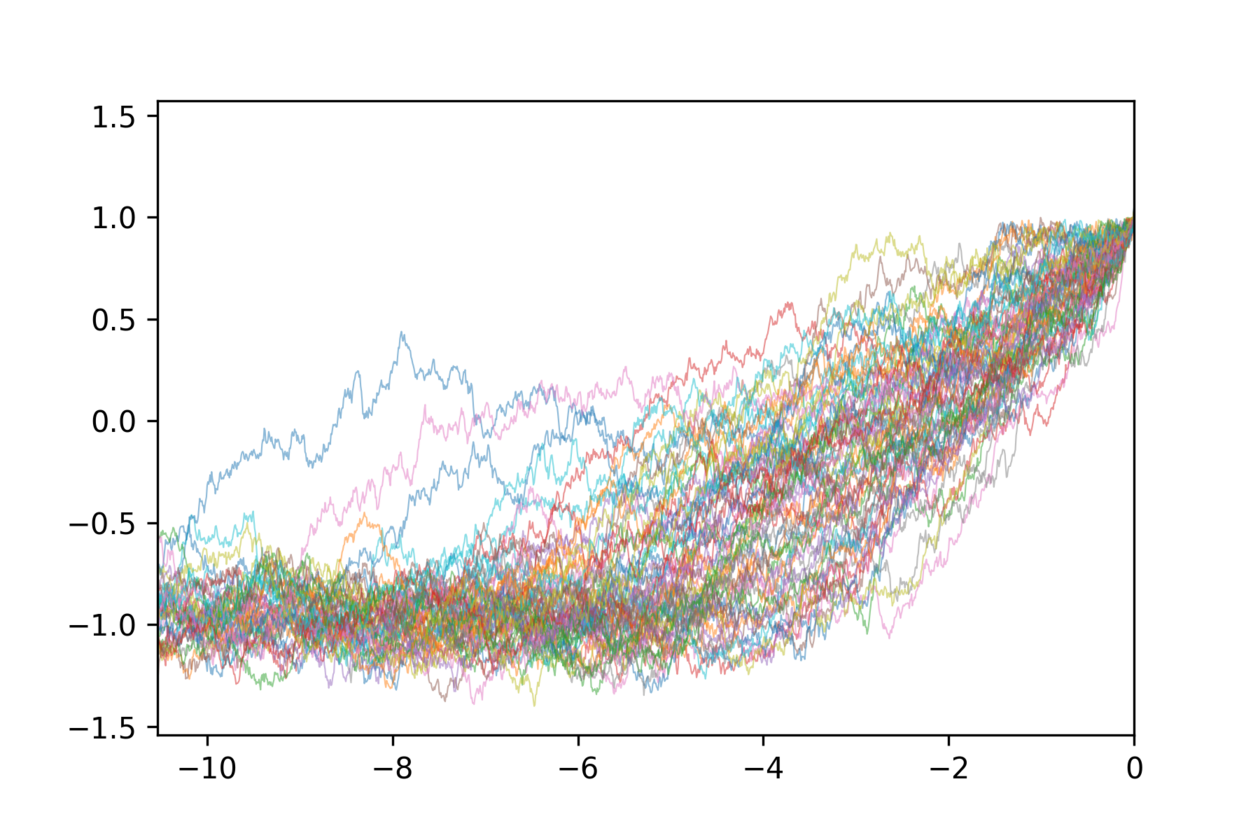
\includegraphics[width=0.5\textwidth]{figures/lez_12_walker_t_path.png}
    \caption{\scriptsize 70 camminatori che raggiungono il punto C (\href{https://github.com/dodogabrie/Sistemi-Complessi/blob/master/python-project/lezione12/MFPT_simulation_py.ipynb}{Link al codice in python}).}
    \label{fig:figures-lez_12_walker_t_path-png}
\end{figure}
\noindent 
Si nota come tutte le traiettorie sembrino seguire un percorso specifico, incanalandosi in una specie di tubo di flusso per arrivare in $x=1$. \\
Questa cosa appare evidente se andiamo a vedere la densità dei punti in cui nei quali è passato il camminatore:
\begin{figure}[H]
    \centering
    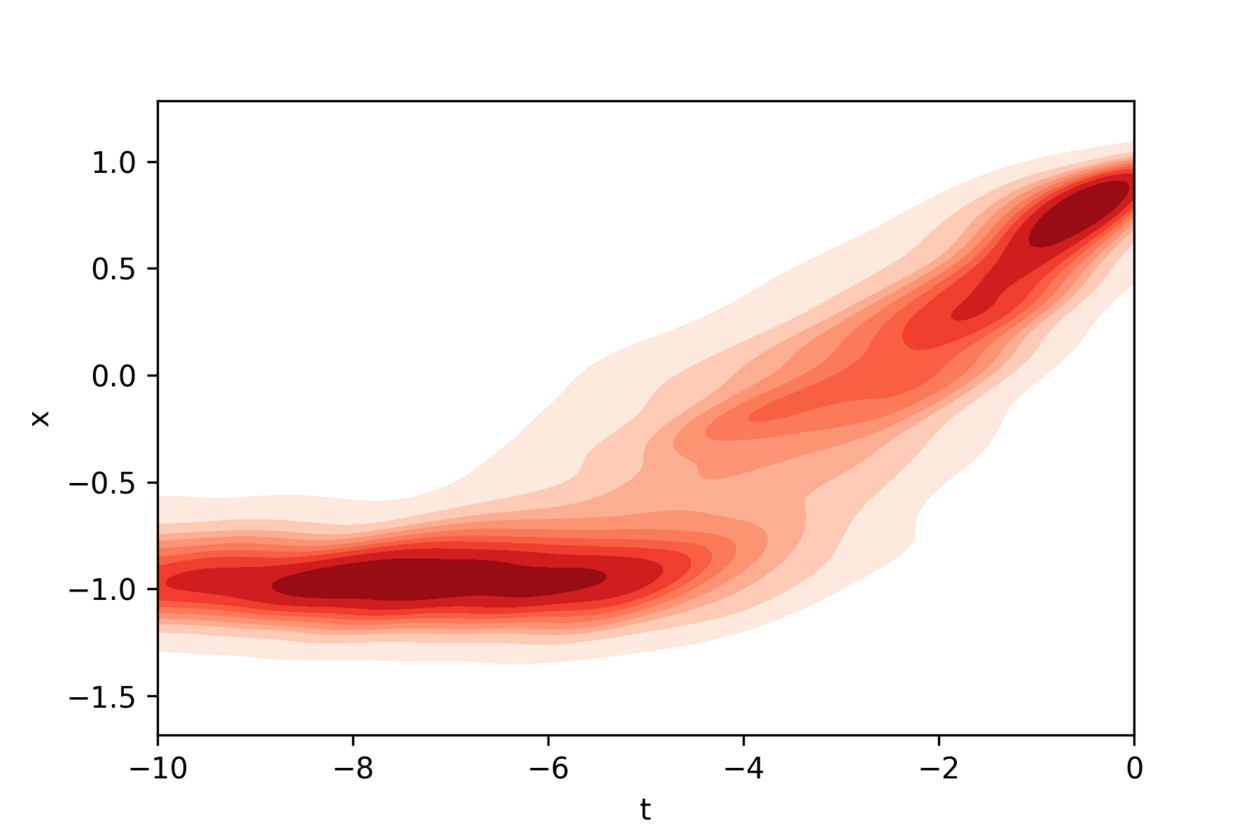
\includegraphics[width=0.5\textwidth]{figures/lez_12_walker_t.png}
    \caption{\scriptsize Densità dei camminatori che riescono a fare il salto nel tempo, si nota che si addensano attorno ad un tubo di flusso (\href{https://github.com/dodogabrie/Sistemi-Complessi/blob/master/python-project/lezione12/MFPT_simulation_py.ipynb}{Link al codice in python})}
    \label{fig:figures-lez_12_walker_t-png-}
\end{figure}
\noindent 
Una cosa molto interessante da notare è la scala temporale, se mediamente un camminatore impiega un tempo di $100$ digit per scappare dalla buca $A$ restringendoci ai soli camminatori che riescono nell'impresa questo tempo risulta essere inferiore a $8$ digit. \\
Questo significa che la sequenza di $dW_n$ che permette il passaggio è molto improbabile, infatti deve essere tale da spingere il camminatore oltre una barriera!\\
Si possono prendere tutte le sequenze di $dW$ che hanno permesso ai $70$ camminatori di attraversare la barriera e valutarne la densità in $x$. Il seguente grafico mostra un istogramma bidimensionale ('countour plot') del rumore in funzione di $x$:
\begin{figure}[H]
    \centering
    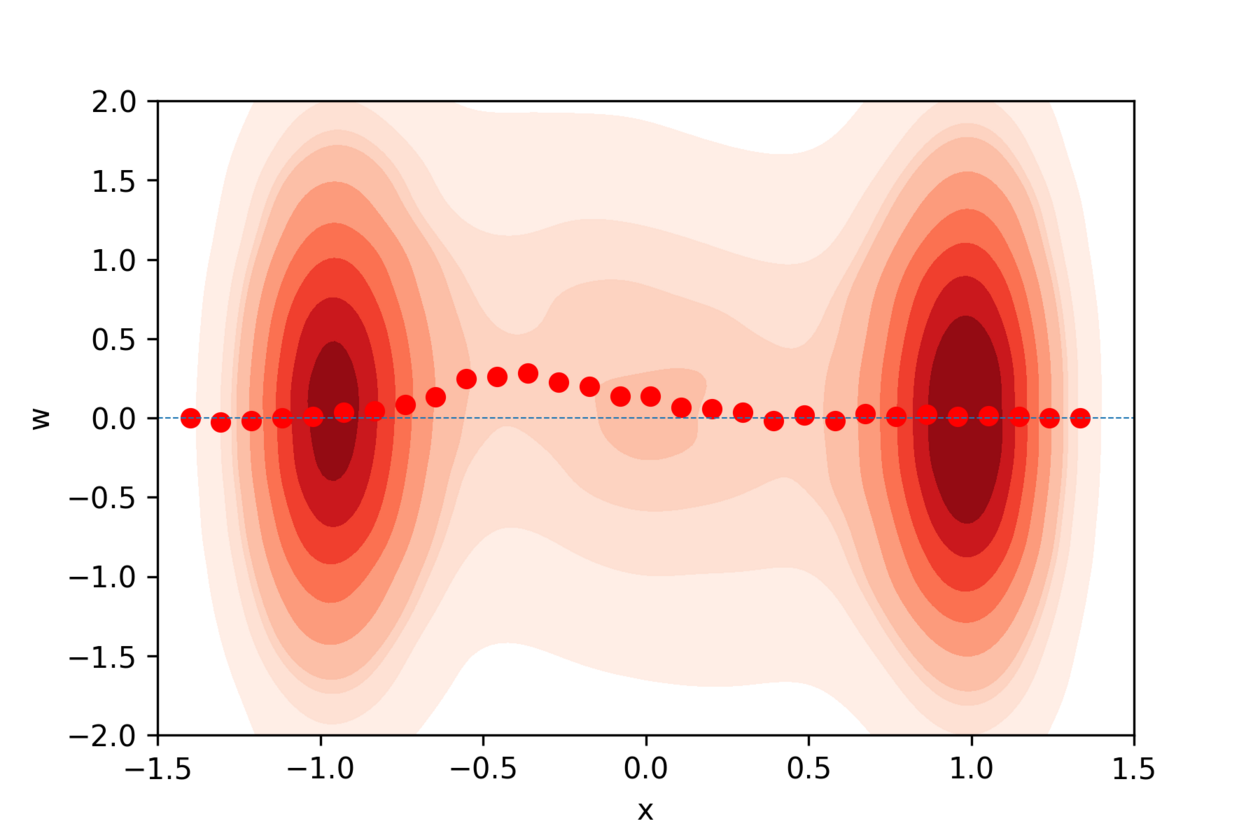
\includegraphics[width=0.5\textwidth]{figures/lez_12_dist.png}
    \caption{\scriptsize Distribuzione del processo stocastico per i camminatori che riescono a fare il salto, notiamo che la media del processo (curva arancione) deve essere diversa da zero (\href{https://github.com/dodogabrie/Sistemi-Complessi/blob/master/python-project/lezione12/MFPT_simulation_py.ipynb}{Link al codice in python}).}
    \label{fig:figures-lez_12_dist-png}
\end{figure}
\noindent
Possiamo notare il fatto che per ottenere una sequenza giusta il rumore debba essere diverso da zero (e positivo) lungo la salita del potenziale. \\
Superata la barriera allora il rumore può gradualmente rilassare: la fatica ormai è fatta. 

\subsection{Hamiltoniana per il MFPT}%
\label{sub:Hamiltoniana per il MFPT}
Riprendiamo l'equazione per il processo in forma discretizzata:
\[
    x_{n+1} = x_n + f(x_n) \Delta t + \sigma \Delta\omega_n = F(x_n) + \xi_n
.\] 
\[
    \left<\xi_n\xi_m\right> = \epsilon\Delta_{nm}
.\] 
Consideriamo sempre l'intervallo $(a,b)$ come sopra. Abbiamo visto che la probabilità di andare da $a$ a $b$ 
\[
    P\left(x_b,t|x_a,0\right)
.\] 
è legata alla probabilità di una "corretta" fluttuazione di $\xi$. \\
Supponiamo di discretizzare il tempo con un passo $\Delta t$:
\[
    t_{i+1} = t_i + \Delta t 	\quad \forall i
.\] 
La probabilità di arrivare in $b$ può essere scritta come una catena di propagatori:
\[\begin{aligned}
    P\left(x_b,t|x_a,t_0\right)=&P\left(x_1,t_1|x_a,t_0\right)\cdot P\left(x_2,t_2|x_1,t_1\right)\cdot \ldots \\
				&\ldots \cdot P\left(x_b,t_b|x_{n-1},t_{n-1}\right)
.\end{aligned}\]
Dove si sfrutta in questo passaggio il fatto che il sistema è markoviano (quindi è lecito scrivere la probabilità composta in questo modo).\\
Notiamo che la probabilità di fare il salto dalla posizione $x_{i}$ a quella $x_{i+1}$ deve essere legato alla probabilità di ottenere il "giusto" $\xi_i$  del processo di Wiener:
\[
    P\left(x_{i+1}, t_{i+1}|x_i,t_i\right) \sim P(\xi_i) 
.\] 
\[
    \text{Con } \xi_i: \quad x_{i+1} = F(x_i) + \xi_i
.\] 
Sia $\gamma$ una fluttuazione ottimale che permette il passaggio da $a$ a $b$.
\[
	\gamma \to \left[\zeta_1, \ldots, \zeta_n\right]
.\] 
La probabilità che tale fluttuazione avvenga avrà la forma (vedi ad esempio la soluzione stazionaria della Lezione \ref{eq:5_staz}):
\[
    P(\gamma) \sim \exp\left(-\frac{S\left[x_1,\ldots,x_n\right]}{\epsilon}\right)
.\] 
\[
    S = \frac{1}{2}\sum_{}^{} \zeta^2_i
.\] 
Quindi il tempo di primo passaggio può essere ricavato dal fatto che
\footnote{La dimostrazione che questa probabilità ed il MFPT sono legati è nel PDF del professore (pathintegral).}
:
\[
    P\left(x_n,t_n = T|x_0,t_0\right) \sim k \exp\left(-\frac{S_{\text{min}}}{\epsilon}\right)
.\] 
Quello che cerchiamo è il minimo dell'azione $S$: $\overline{S}$, ovvero la sequenza $\gamma$ che massimizza la probabilità di fare il salto $a\to b$.\\
Per risolvere il problema di minimo possiamo utilizzare un set di moltiplicatori di Lagrange $\lambda_i$.
\[
    \overline{S} = \frac{1}{2}\sum_{i}^{} \zeta^2_i + \lambda_i \left[x_{i+1}-F(x_i)- \zeta_i\right]
.\] 
Risolvendo il problema dei moltiplicatori si ottiene:
\[\begin{aligned}
    &1. \quad x_{n+1} = F(x_n) + \lambda_n\\
    &2. \quad \lambda_{n+1}=\left[\left.\frac{\partial F}{\partial x_i} \right|_{i = n+1}\right]^{-1}\lambda_n
.\end{aligned}\]
Passiamo a tempi continui, chiamiamo $\Delta t = h$, dalla prima equazione si ottiene che
\footnote{Non mi torna l'$h$, mi pare sparita\ldots}
:
\[
    x_{n+1} = x_n + h f(x_n) + \lambda_n \implies  \dot{x} = f + \lambda
.\] 
La seconda equazione può essere manipolata considerando la definizione di $F$:
\[
    F(x_n) = x_n+hf(x_n) \quad \implies  \quad  \frac{\partial F}{\partial x} = 1+hf'
.\] 
Sostituendo questa nella (2.) e sommando e sottraendo $\lambda_n$ si arriva a:
\[
    \dot{\lambda} =  - f'\lambda
.\] 
Ci siamo ricondotti a due equazioni da integrare con le opportune condizioni al contorno:
\begin{redbox}{Equazioni di Hamilton per il sistema}
\[
    \begin{cases}
	\dot{x} = f(x) + \lambda\\
	\dot{\lambda } = - f'(x) \lambda
    \end{cases}
.\]     
\end{redbox}
\noindent
l'Hamiltoniana che corrisponde a queste equazioni è della forma:
\[
    \lambda  \to p \quad \implies  \quad H = \frac{p^2}{2} + pf
.\] 
Infatti vale che:
\[
    \begin{cases}
	\dot{x} = \left[x,H\right]\\
	\dot{p} = \left[p,H\right]
    \end{cases}
.\] 
Le condizioni al contorno che possiamo usare per risolvere sono 
\[
    x(t=0) = a; \quad x(t = t_n) = b
.\] 
Il problema può essere risolto con il calcolo della azione, sappiamo che l'azione di un sistema è legata alla lagrangiana dalla seguente:
\[
    \dot{S} = \mathcal{L} = \frac{\partial H}{\partial P} P - H
.\] 
Quindi operativamente basta integrare la lagrangiana per ottenere la $S$, minimizzarla per avere la $P$, visto che $P$ è proporzionale al tempo di primo passaggio $T$. 
\subsubsection{Applicazione del metodo ad un potenziale $U(x)$}%
\label{subsub:Applicazione del metodo ad un potenziale $U(x)$}
Prendiamo l'equazione per l'incremento di $x$:
\[
    dx = - U' dt + \sqrt{\epsilon} d\omega
.\] 
In cui si ha che, come già accennato $-U' = f$:
\[
    H = \frac{p^2}{2}-pU'
.\] 
Risolviamo le equazioni di Hamilton:
\[
    \begin{cases}
	\dot{x} = -U' + p\\
	\dot{p} = U''p
    \end{cases}
.\] 
Possiamo derivare la prima e sostituire $\dot{p}$ dalla seconda:
\[\begin{aligned}
    \ddot{x} &= -U'' \dot{x} + \dot{p} =\\
	      & = - U'' \dot{x} + U'' p = \\
	      & = U''\left(- \dot{x} + p\right) = U'U''
.\end{aligned}\]
Quindi ne emerge che $U'U''$ ha la struttura di una "forza"
\footnote{Per unità di massa eventualmente\ldots}, 
vediamo qual'è la forma grafica di tutte le quantità in gioco.
%\begin{figure}[H]
    \centering
    \begin{tikzpicture}
	\begin{axis}[
	    width=7cm,
	    height=4cm,
	    xmin= -2, xmax= 2,
	    ymin= 0, ymax = 0.4,
	    axis lines = middle,
	    x label style={at={(axis description cs:1,-0.01)},anchor=north},
	    y label style={at={(axis description cs:0.5,1)},anchor=south},
	    xlabel={$x$},
	    ylabel={$U(x)$ },
	    xtick={0, 1, -1},
	    xticklabels={$0$, $1$, $-1$},
	    ytick={0},
	    yticklabel={$0$},
	    ]
	    \addplot[domain=-3:3, samples=500]{-x^2/2*(1-x^2/2) + 0.3};
	    \node (C) [mark=dot] at (axis cs: 1, 0.1) {$C$};
	    \node (B) [mark=dot] at (axis cs: 0.1, 0.325) {$B$};
	    \node (A) [mark=dot] at (axis cs: -1, 0.1) {$A$};
	\end{axis}
    \end{tikzpicture}
    \begin{tikzpicture}
	\begin{axis}[
	    width=7cm,
	    height=4cm,
	    xmin= -2, xmax= 2,
	    ymin= -0.4, ymax = 0.4,
	    axis lines = middle,
	    x label style={at={(axis description cs:1,0.49)},anchor=north},
	    y label style={at={(axis description cs:0.5,1)},anchor=south},
	    xlabel={$x$},
	    ylabel={$U'(x)$ },
	    xtick={0, 1, -1},
	    xticklabels={$0$, $1$, $-1$},
	    ytick={0},
	    yticklabel={$0$},
	    ]
	    \addplot[domain=-3:3, samples=500]{-x+x^3};
	\end{axis}
    \end{tikzpicture}
    \begin{tikzpicture}
	\begin{axis}[
	    width=7cm,
	    height=4cm,
	    xmin= -2, xmax= 2,
	    ymin= -0.4, ymax = 0.1,
	    axis lines = middle,
	    x label style={at={(axis description cs:1,0.79)},anchor=north},
	    y label style={at={(axis description cs:0.5,1)},anchor=south},
	    xlabel={$x$},
	    ylabel={$-(U'(x))^2$ },
	    xtick={0, 1, -1},
	    xticklabels={$0$, $1$, $-1$},
	    ytick={0},
	    yticklabel={$0$},
	    ]
	    \addplot[domain=-2:2, samples=500]{-1*(-x+x^3)^2};
	\end{axis}
    \end{tikzpicture}
    \caption{\scriptsize Potenziale in cui vivono i camminatori e la sua derivata strettamente legata alla forza sul camminatore.}
    \label{fig:12_pot_der}
\end{figure}

\noindent
Il potenziale efficace che mi genera la forza $U'U''$ è 
\[
    U_{\text{eff}} = -\frac{1}{2}\left(U'(x)\right)^2
.\] 
Questo perché effettuando tale derivata si riottiene l'equazione sopra ai grafici, si ha quindi:
\[
    \ddot{x} = \frac{\text{d} }{\text{d} x} \left(-\frac{1}{2}(U'(x) ) ^2\right)
.\] 
Quindi se integriamo questa equazione in $x$ si scopre che il moto avviene ad una energia costante $E$, di fatto si trova la conservazione della energia meccanica:
\[
    \frac{1}{2} \dot{x}^2 - \frac{1}{2} U'^2 = E
.\] 
Notiamo che il grafico che conta ai fini del moto (della velocità del camminatore) è il terzo in Figura \ref{fig:12_pot_der}.\\
Poniamoci nel caso di energia nulla, si ottiene che
\begin{equation}
    \dot{x} = \pm U'
    \label{eq:12_moto}
\end{equation}
Fisicamente nel sistema	si ha che nel tratto di salita sul potenziale l'equazione del moto è 
\[
    \dot{x} =  + U'
.\] 
Mentre nel tratto di successiva discesa vale l'equazione con il meno. In conclusione si ha per l'esempio discusso in questa lezione:
\[
    \begin{cases}
	\dot{x} = + U' & x<0\\
	\dot{x} = -U' & x\ge 0
    \end{cases}
\] 
Adesso possiamo confrontare questa equazione con quella di partenza di questa lezione (è la \ref{eq:12_beg} riscritta):
\[
    \dot{x} = -U' + \xi
.\] 
Quindi notiamo che nella parte di discesa il moto stocastico $\xi$ è irrilevante, infatti abbiamo l'equazione di partenza con $\xi=0$. Nella parte di salita invece il moto stocastico è tale da invertire di segno all'equazione per $ \dot{x}$.\\
Proprio per questo motivo le sequenze che permettono il passaggio sopra la barriera sono difficili da generare.
Possiamo allora confrontare questa soluzione con le simulazioni mostrate sopra, generando la traiettoria di Equazione \ref{eq:12_moto} si ottiene:
\begin{figure}[H]
    \centering
    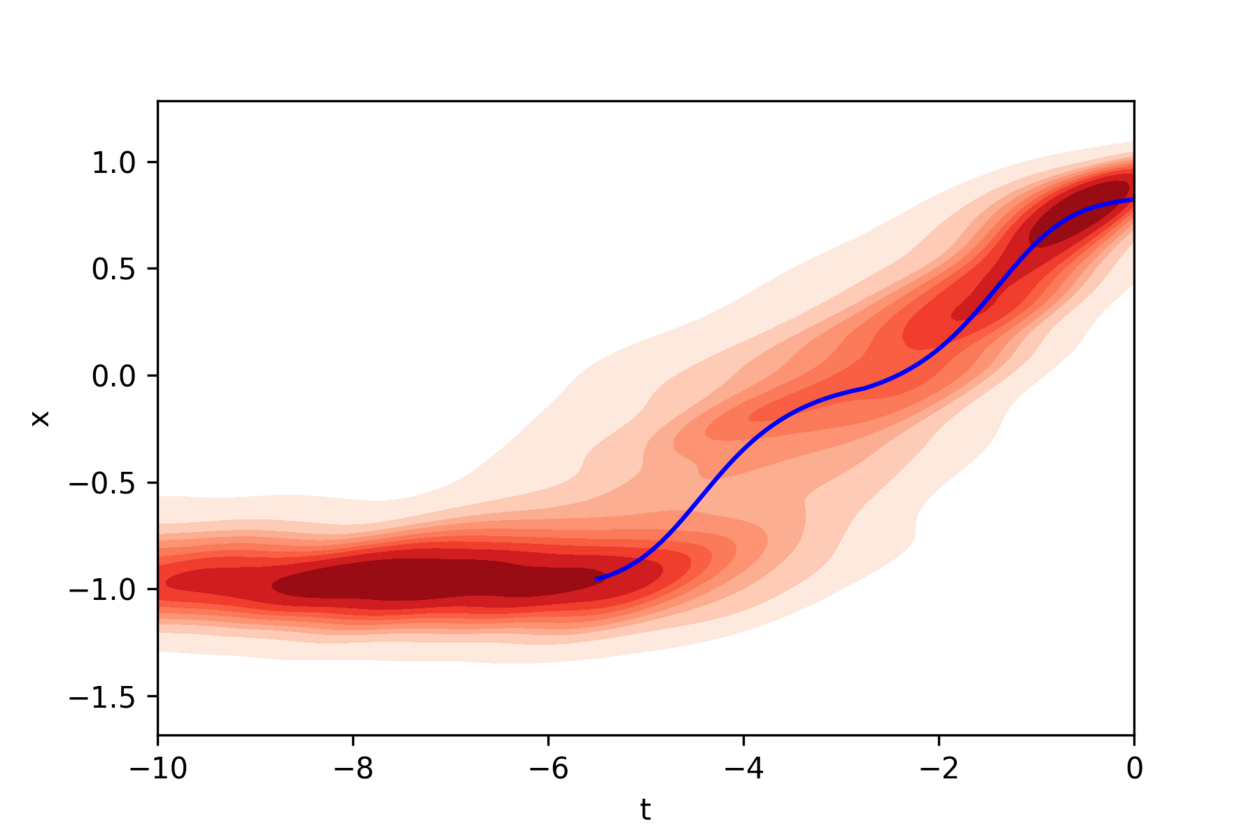
\includegraphics[width=0.5\textwidth]{figures/lez_12_walker_t_theory.png}
    \caption{\scriptsize Confronto tra simulazione dei camminatori e curva teorica di un camminatore che minimizza l'azione (\href{https://github.com/dodogabrie/Sistemi-Complessi/blob/master/python-project/lezione12/MFPT_simulation_py.ipynb}{Link al codice in python}).}
    \label{fig:figures-lez_12_walker_t_theory-png}
\end{figure}
\noindent
Notiamo che la curva teorica è compatibile con il flusso di camminatori
\footnote{Sul plot è necessario precisare che il camminatore con la legge $\dot{x} = \pm U'$ raggiunge i punti interessanti $x=0$, $x=+1$ in un tempo infinito. Il moto è stato tagliato per renderlo ragionevolmente simile all'andamento delle simulazioni. Guardando il file del professore suppongo abbia fatto lo stesso. Questo falsifica parzialmente la validità del risultato.
}
.\\
Risolvendo le equazioni di Hamilton per $p (=\lambda)$ si ottiene anche il seguente andamento teorico:
\begin{figure}[H]
    \centering
    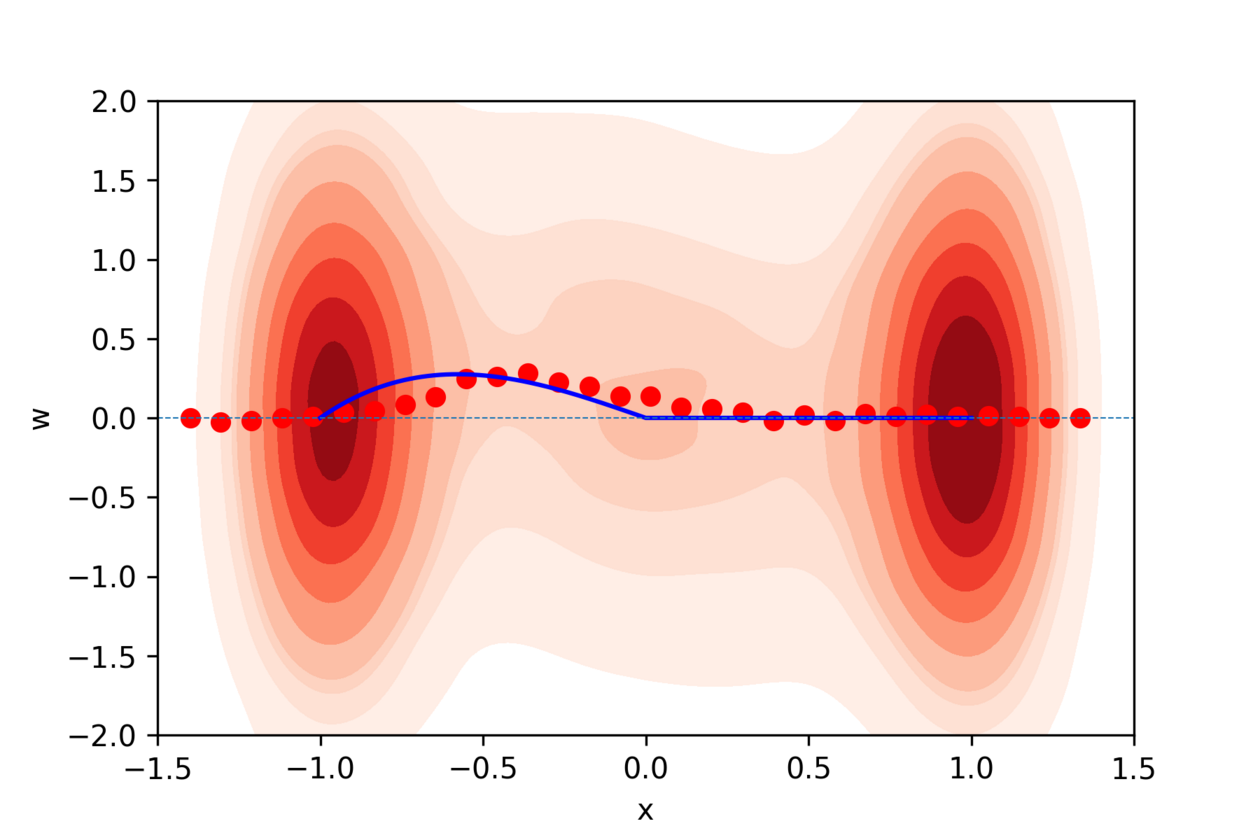
\includegraphics[width=0.5\textwidth]{figures/lez_12_dist_theory.png}
    \caption{\scriptsize Confronto tra media predetta del processo di Wiener e media ottenuta dalle simulazioni, tutto in funzione di $x$ (\href{https://github.com/dodogabrie/Sistemi-Complessi/blob/master/python-project/lezione12/MFPT_simulation_py.ipynb}{Link al codice in python}).}
    \label{fig:figures-lez_12_dist_theory-png}
\end{figure}
\noindent
Per ottenere questo risultato è stato necessario, a livello computazionale, di moltiplicare la soluzione $p$ per il fattore $dt / \sqrt{\epsilon}$. 
Senza far questo il rumore ottenuto verrà fuori scala rispetto a quello simulato.\\
Possiamo notare una non conformità nei pressi di $x=0$, questo può essere dovuto al campione statistico di simulazioni
\footnote{Noto che il campione può essere ampliato scrivendo una funzione e chiamandola più volte. In questo modo si risolve il problema della memoria occupata in eccesso a causa della matrice di numeri random e di quella delle posizioni iniziali.}.\\
Possiamo adesso utilizzare questo modello per confrontarlo con le simulazioni. In figura \ldots si mostra una simulazione di camminatori che raggiungono $x= 0.2$ per poi rilassare.
\begin{figure}[H]
    \centering
    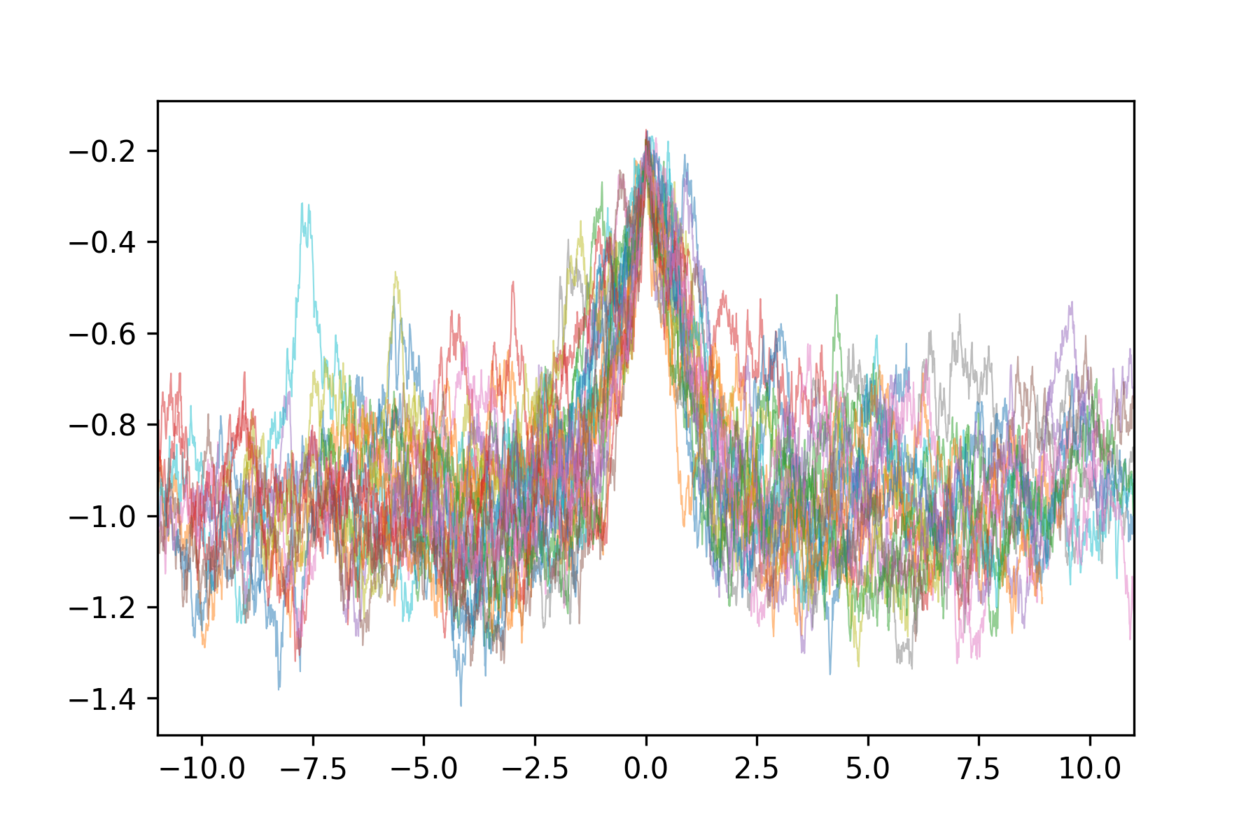
\includegraphics[width=0.5\textwidth]{figures/lez_12_walker_t_cutted.png}
    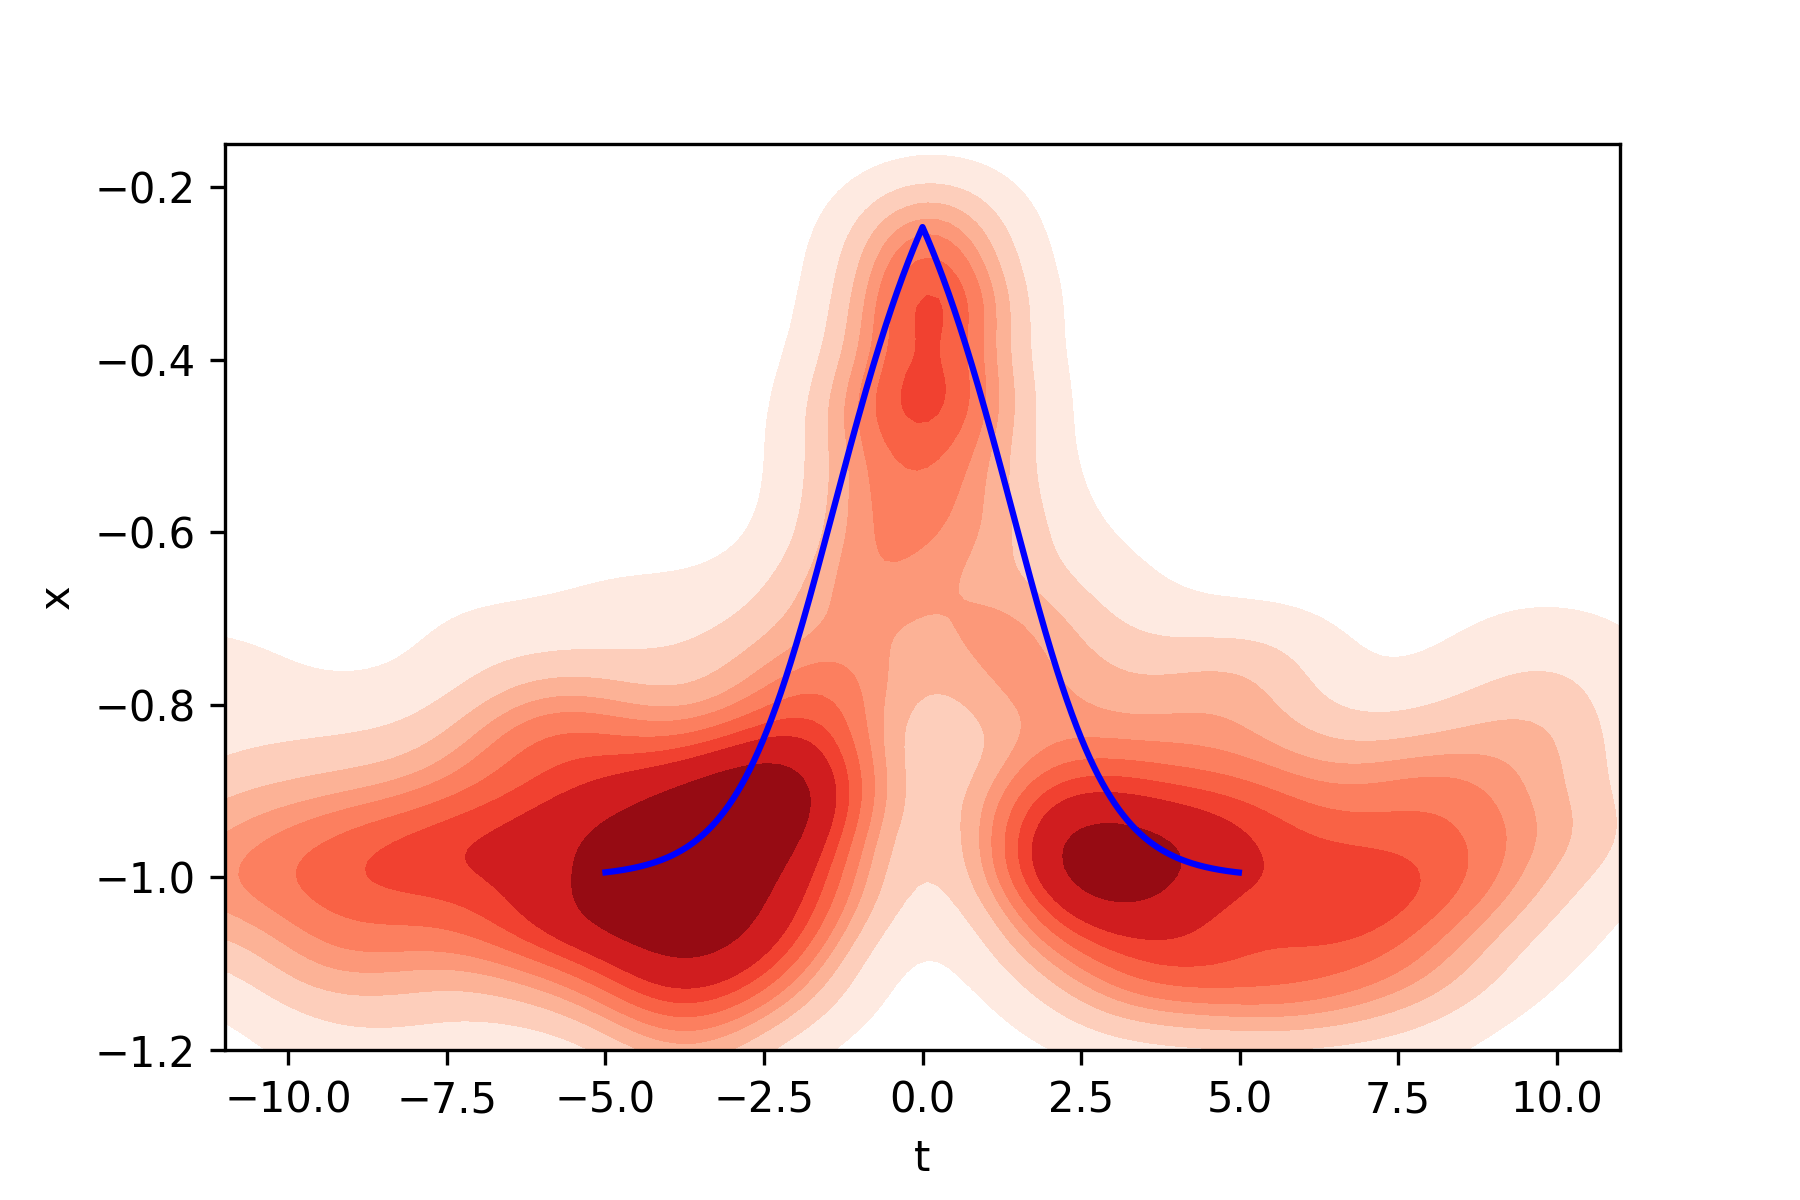
\includegraphics[width=0.5\textwidth]{figures/lez_12_walker_t_cutted_theory.png}
    \caption{\scriptsize Camminatori selezionati che arrivano a $x = 0.2$ per poi rilassare e distribuzione in densità dei camminatori con la curva teorica in blu (\href{https://github.com/dodogabrie/Sistemi-Complessi/blob/master/python-project/lezione12/MFPT_simulation_py.ipynb}{Link al codice in python}).}
    \label{fig:figures-lez_12_walker_t_cutted_theory-png}
\end{figure}
\noindent
Si nota come i camminatori si distribuiscono lungo due cammini che corrispondono a $\dot{x} = \pm U'$.
\subsection{Da cammino ottimale a MFPT}%
\label{sub:Da cammino ottimale a MFPT}
Abbiamo detto che il contributo stocastico arriva solo nella parte di salita, possiamo usare questo per calcolare la derivata della azione:
\begin{equation}
\begin{aligned}
    \dot{S} =& \frac{\partial H}{\partial p} p - H = \\
            =& \left(p-U'\right)p - \frac{1}{2}p^2+pU' = \\
	    =& \frac{1}{2}p^2 = \\
	    =& \frac{1}{2}\left(\dot{x}+U'\right)^2
.\end{aligned}
\label{eq:12_action}
\end{equation}
Sostituendo la soluzione per $\dot{x}$ ottenuta prima si ha che:
\[
    \dot{S} = 
    \begin{cases}
	2(U') ^2 & \text{ Salita}\\
	0        & \text{ Discesa}
    \end{cases}
    = 2 \dot{x}^2 = 2\dot{x}U'
.\] 
A questo punto possiamo integrare per ottenere l'azione:
\[\begin{aligned}
    S_{min} =& \int\dot{S}dt = 
             2\cdot \int_{a}^{b} \dot{x}U'dt = \\
            =& 2  \int_{a}^{b} \left(\frac{\text{d} U}{\text{d} t} \right)dt =
	     2(U_b-U_a)  
.\end{aligned}\]
Quindi il tempo di primo passaggio, come già accennato, sarà proporzionale a:
\[\begin{aligned}
    \text{MFPT} \sim& \exp\left(-\frac{S_{\text{min}}}{\epsilon}\right) =
    \exp\left(-\frac{2(U_b-U_a)}{2D}\right) =\\
    =&\exp\left(-\frac{U_b-U_a}{D}\right)
.\end{aligned}\]
Che è proprio la legge di Harrenius trovata nella lezione precedente.\\
Il metodo esposto per il tempo di primo passaggio è molto generale, possiamo applicarlo anche a casi N-dimensionali.
\subsection{Calcolo del MFPT in 2D: Oscillatore di Van Der Pol invertito}%
\label{sub:Calcolo del MFPT in 2D}
Prendiamo un sistema bidimensionale con le seguenti SDE per il moto dei camminatori:
\[\begin{aligned}
    & dx = ydt\\
    & dy = \left(-2\eta (1-x^2) y - x\right)dt + \sqrt{ 4\eta T} d\omega
.\end{aligned}\]
Questo sistema è un famoso oscillatore, studiato per descrivere l'andamento della corrente nelle valvole.
\begin{figure}[H]
    \centering
    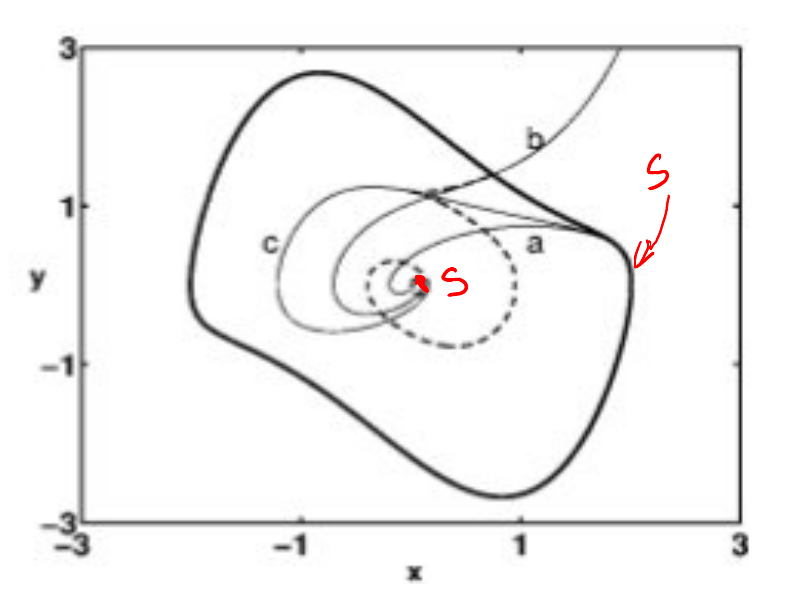
\includegraphics[width=0.4\textwidth]{figures/lez_12_Van_Der_Pol_oscillator.png}
    \caption{\scriptsize Oscillatore di Van Der Pole nello spazio $x, y$.}
    \label{fig:figures-lez_12_Van_Der_Pol_oscillator-png}
\end{figure}
\noindent
La linea scura in figura è un \texttt{Ciclo limite instabile}, inserendo un camminatore in questa traiettoria ( con le condizioni iniziali opportune e rimuovendo la parte stocastica della equazione ) questo rimarrebbe eternamente su di essa. Un camminatore che parte all'interno collassa sull'origine $S$, all'esterno invece i punti scappano via verso $r\to \infty$.\\
Possiamo immaginare quindi questo sistema come un potenziale dalla forma "vulcanica", in cui il ciclo limite instabile corrisponde al cratere.\\
Possiamo chiederci quanto impieghi un camminatore inizializzato all'interno ad arrivare sul bordo del cratere ( come risalire un potenziale bidimensionale ).\\
Potremmo tentare di risolvere il problema come fatto in precedenza:
\begin{itemize}
    \item Trovare l'equazione di FK.
    \item Scrivere l'equazione del tempo di primo passaggio.
    \item Risolvere l'equazione alle derivate parziali.
\end{itemize}
Il problema è che, anche se si riuscisse a risolvere l'equazione alle derivate parziali, non è affatto banale inserire le condizioni al contorno (ne analiticamente ne numericamente).\\
Il vantaggio del metodo è che possiamo scrivere una Hamiltoniana per il sistema:
\[
    H = yp_x + \left[-2\eta (1-x^2) y - x\right]p_y + \frac{1}{2}(4\eta T) p_y^2
.\] 
Possiamo dire che i camminatori partono dal fondo del cratere $S$, si risolve il problema trovando i cammini che arrivano al bordo del cratere e poi si minimizzano questi cammini (si minimizza l'azione). \\
Le traiettorie $a$, $b$ in figura \ref{fig:figures-lez_12_Van_Der_Pol_oscillator-png} sono state trovate dal professore ed arrivano tangenti al ciclo limite.\\
Possiamo cercare di capire se il sistema ha una distribuzione di equilibrio, questo equivale a capire se il sistema presenta il bilancio dettagliato.\\
La condizione del bilancio dettagliato è soddisfatta se vale la \ref{eq:11_rot}. Esplicitando tale conto si ha:
\[
    f_x = y \qquad f_y = -2\eta (1-x^2) y - x
.\] 
\[
    \frac{\partial f_x}{\partial y} = 1 \neq \frac{\partial f_y}{\partial x} = 4\eta xy - 1
.\] 
L'equazione al rotore nullo non è soddisfatta, quindi il sistema non presenta il bilancio dettagliato.\\
L'assenza del bilancio dettagliato non influisce sul calcolo del MFPT, tuttavia la traiettoria di fuga ottimale non è univoca (come invece si avrebbe con il bilancio dettagliato) e di conseguenza si sviluppa una cuspide all'interno del ciclo limite instabile (nello spazio delle fasi vediamo più di un cammino partendo dallo stesso punto).
\begin{exmp}[]
    Prendiamo la seguente SDE:
    \[
	 dx = (-U'(x) + A\sin (wt) ) dt + \sqrt{\epsilon} d\omega    
    .\] 
    La possiamo spezzare in due termini:
    \[
	\begin{cases}
	 dx_1 = w dt\\
	 dx_2 = (-U'(x_2) + A\sin (x_1) ) dt + \sqrt{\epsilon} d\omega    
	\end{cases}
    \] 
    Le equazioni di Hamilton-Jacobi ricordiamo essere:
    \[
        \begin{cases}
            \dot{x}= -U' + p\\
	    \dot{p} = U'' p
        \end{cases}
    \] 
    Essendo in due dimensioni non abbiamo quantità scalari, ad esempio:
    \[
        -U' = 
	\begin{pmatrix} 
	    w  \\
	    A\sin (x_1) -U'(x_2) 
	\end{pmatrix} 
    \] 
    Quindi esisterà anche un tensore delle derivate seconde, le cui componenti non nulle sono:
    \[\begin{aligned}
	& U''_{x_1, 2} = -\partial_{x_1}w + \partial_{x_1}(A\sin (x_1)) = -A\cos (x_1) \\
	& U_{x_2,2} = -\partial_{x_2} (-U'(x_2) ) 
    \end{aligned}\]
    In cui si è cambiato segno perché avevamo $-U'$. Alla fine si ottiene un oggetto del tipo:
    \[
        U'' = 
	\begin{pmatrix} 
	    0  &  -A\cos (x_1) \\
	    0  &  d^2U/d(x_2)^2
	\end{pmatrix} 
    .\] 
    In conclusione abbiamo il seguente set di equazioni per il moto:
    \[\begin{aligned}
	&\dot{x}_1 = w\\
	&\dot{x}_2 = -U'(x_2) + A \sin (x_1) + p_2 \\
	& \dot{p}_1 = -A\cos (x_1) \cdot p_2\\
	& \dot{p}_2 = \frac{\text{d}^2}{\text{d} (x_2)^2 }(U) \cdot  p_2
    .\end{aligned}\]
    L'Hamiltoniana si scrive come:
    \[
	H = w p_1 + \frac{(p_2)^2}{2} + p_2(A\sin (x_1) - U'(x_2) ) 
    .\] 
    Ricordiamo che di ha questa forma perché dev'essere:
    \[
        \frac{\text{d} p}{\text{d} t} = - \frac{\partial H}{\partial q}  
	\qquad \qquad
	\frac{\text{d} q}{\text{d} t} = \frac{\partial H}{\partial p} 
    .\] 
    Possiamo estrarre l'azione dalla \ref{eq:12_action}, si ottiene:
    \[\begin{aligned}
	\dot{S} = p\partial_{p}H-H=\ldots=\frac{(p_2)^2}{2}
    .\end{aligned}\]
    Simulando il moto con le equazioni di Hamilton si possono ottenere delle traiettorie come quelle in Figura \ref{fig:figures-lez_12_strange_motion-png}.
    \begin{figure}[H]
        \centering
	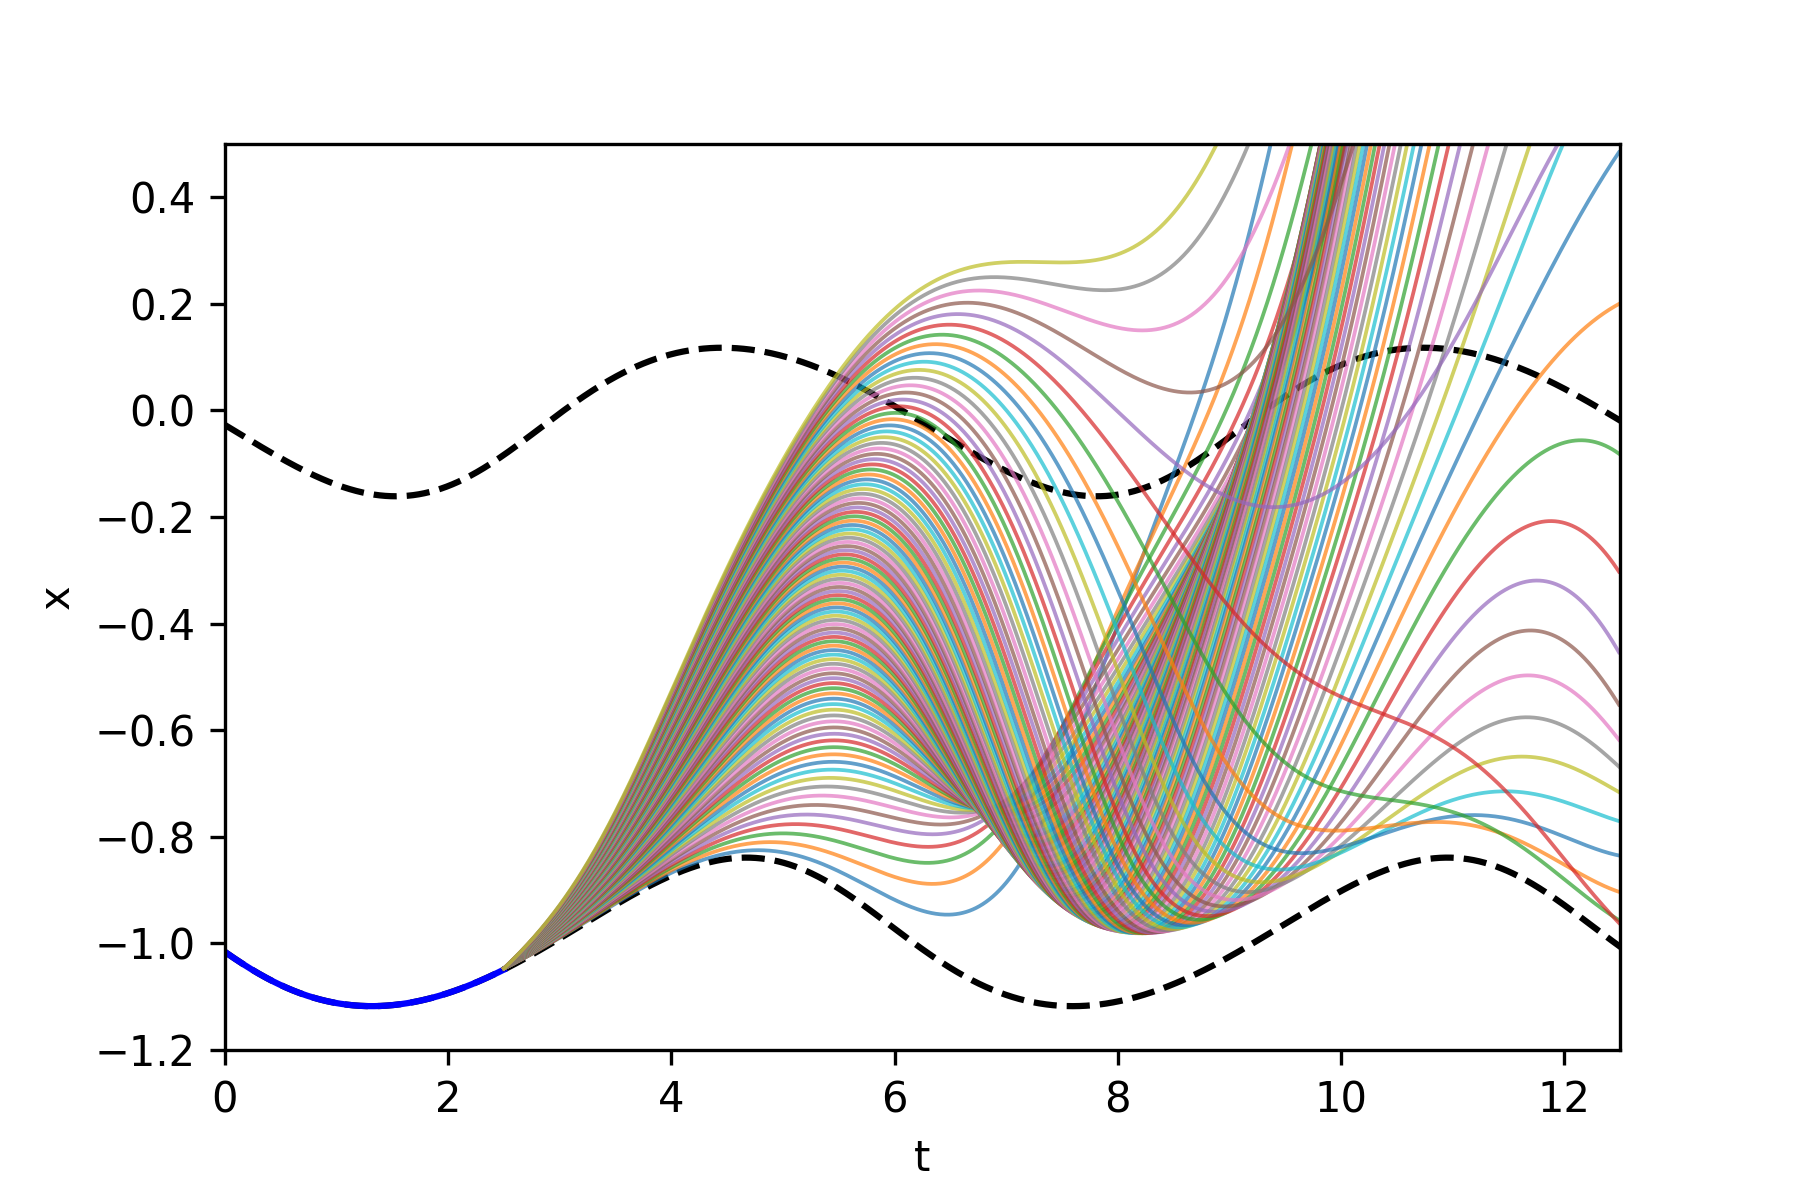
\includegraphics[width=0.5\textwidth]{figures/lez_12_strange_motion.png}
	\caption{\scriptsize Traiettorie di fuga generate con le equazioni del moto. La traiettoria che minimizza l'azione (tra le condizioni iniziali testate) è evidenziata in rosso. Notiamo per arrivare in un punto nei pressi della cuspide ci siano più traiettorie possibili, questo è tipico dei sistemi che non hanno il bilancio dettagliato.}
        \label{fig:figures-lez_12_strange_motion-png}
    \end{figure}
    \noindent
    Per generare tali traiettorie c'è bisogno di un "delicato" lavoro computazionale.
    Creare la routine per i camminatori è semplice, meno semplice è la scelta delle condizioni iniziali.
    Il sistema è estremamente sensibile alla scelta di $w, A$ e tutte le variabili del moto $p_i, x_i$. \\
    Alcune traiettorie in figura sembrano rilassare, questa è solo una "illusione", infatti nelle oscillazioni successive le traiettorie fuggono tutte, d'altronde il modello scelto serve "solo" a descrivere le traiettorie di fuga.\\ 
    Avendo la sequenza dei $p_2$ è possibile calcolare anche l'azione complessiva su ogni percorso, il risultato che si ottiene è il seguente:
    \begin{figure}[H]
        \centering
	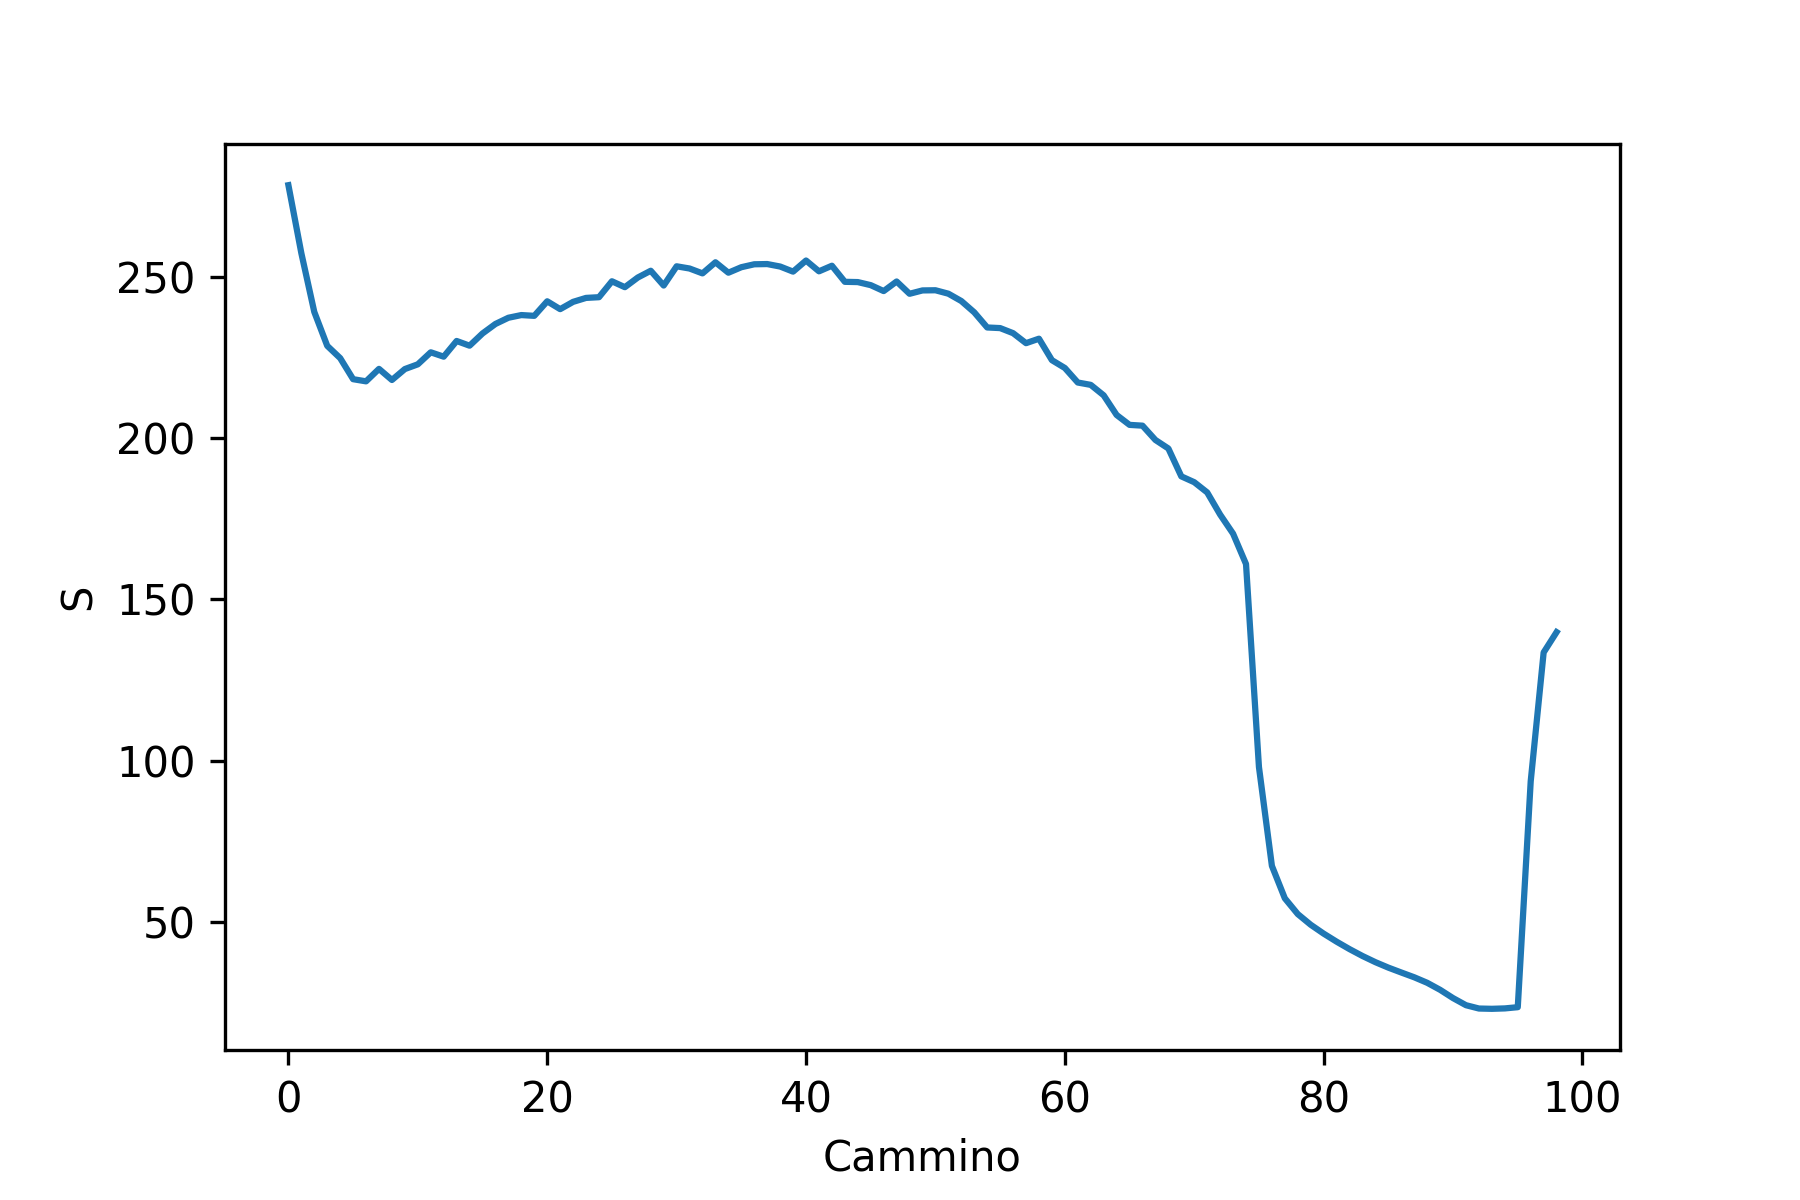
\includegraphics[width=0.5\textwidth]{figures/lez_12_strange_motion_action.png}
	\caption{\scriptsize Azione al variare del camminatore i-esimo. Notiamo l'evidenza di un minimo corrispondente alla curva rossa in figura \ref{fig:figures-lez_12_strange_motion-png}. La possibilità di stimare l'azione minima permette il calcolo del tempo di primo passaggio.}
        \label{fig:figures-lez_12_strange_motion_action-png}
    \end{figure}
    \noindent 
    Il grafico precedente non rispecchia a pieno la vera azione di tutti i camminatori in quanto tutti i moti che scappano dal sistema sono stati troncati per evitare l'overflow, tuttavia possiamo affermare che l'azione di questi camminatori fuggenti è stata sicuramente sottostimata osservando le equazioni di Hamilton.
\end{exmp}
\noindent
Il metodo per trovare le traiettorie di fuga (e quindi il MFPT) è molto potente quando il sistema presenta un "contorno" complicato, può essere applicato addirittura ad un bordo frattale come il set di Julia.
\begin{ex}[Camminatore con bordo dato dal set di Julia]
    Il set di Julia è un bordo frattale, le equazioni agli incrementi per il set sono:
    \[\begin{aligned}
	&x_{n+1} = x^2_n - y^2_n + ax_n + \xi_{x_n}\\
	& y_{n+1}= 2x_ny_n + ax_n + by_n + \xi_{y_n}
    .\end{aligned}\]
    In cui si inserisce un rumore per entrambi gli assi tale che:
    \[
        \left<\xi_{i_n}\xi_{j_n}\right> = \epsilon\delta_{ij}\delta_{nm}
    .\] 
    Il metodo si applica anche a questo bordo senza problemi, se si prova a fare il calcolo si ottiene:
    \begin{figure}[H]
        \centering
	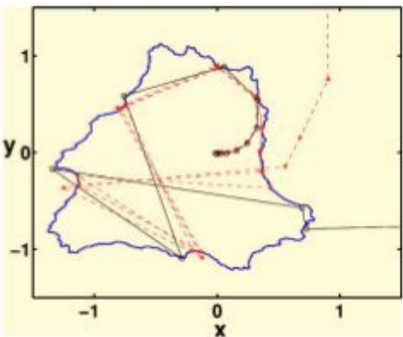
\includegraphics[width=0.4\textwidth]{figures/lez_12_Julia_set.png}
	\caption{\scriptsize Set di Julia con cammino di fuga teorico (tratteggiato) e simulato (nero sottile).}
        \label{fig:figures-lez_12_Julia_set-png}
    \end{figure}
    \noindent
\end{ex}
\noindent
\begin{exmp}[Processo di Ornstein-Ulhenback]
   Se prendiamo un processo di OU possiamo fare gli stessi ragionamenti dell'esempio precedente, partiamo dalle equazioni del processo:
   \[\begin{aligned}
       & dx = f(x) dt + y dt \\
       & dy = - \gamma  y dt + \gamma\epsilon dW
   .\end{aligned}\]
   Risolvendo si arriva alle equazioni di Hamilton-Jacoby:
   \[\begin{aligned}
       & \dot{x}=f(x) + y\\
       & \dot{y}= -\gamma y + p_y\\
       & \dot{p}_x = -f'(x) p_x\\
       & \dot{p}_y=p_x - \gamma p_y
   .\end{aligned}\]
   Ed il problema è risolto.
\end{exmp}
\noindent
\subsection{MFPT applicato allo studio delle glaciazioni}%
\label{sub:MFPT applicato allo studio delle glaciazioni}
Si è notato che l'alternanza tra glaciazioni e periodi caldi ha lo stesso periodo della variazione dell'eccentricità dell'orbita terrestre.\\
Possiamo fare una premessa: la temperatura della terra subisce un feedback negativo per le variazioni di temperatura.
\begin{itemize}
    \item Se la temperatura diminuisce cade la neve ed aumenta il potere riflettente della terra, quindi la temperatura diminuisce ancor di più.
    \item Se la temperatura aumenta il ghiaccio si scioglie e si ha il viceversa.
\end{itemize}
Quindi possiamo immaginare la funzione che determina la temperatura sulla terra come un potenziale a doppia buca (sempre lui, Figura \ref{fig:double_hole_pot}) i quali minimi corrispondono al periodo di caldo e di freddo.\\
Quello che potrebbe fare l'eccentricità è abbassare o alzare uno dei due minimi in funzione della distanza dal sole.\\
Possiamo allora scrivere delle equazioni per la probabilità di essere nel caldo o nel freddo come:
\[\begin{aligned}
    &\dot{P}_f = - \omega_{fc}P_f + \omega_{cf}P_c\\
    & \dot{P}_c =  +\omega_{fc}P_f - \omega_{cf}P_c
.\end{aligned}\]
In cui le $\omega_{ij}$ sono le probabilità di passare da $i$ a $j$.
Visto che l'eccentricità è oscillante possiamo modellizzare questa probabilità con una oscillazione avente lo stesso periodo della eccentricità:
\[
    \omega_{fc /cf} \sim \exp\left(-\frac{U}{T}\mp \frac{A\cos (wt) }{T}\right)
.\] 
Con $T$ temperatura media.\\
Adesso sfruttiamo la proprietà:
\[
    P_f + P_c = 1
.\] 
E approssimiamo l'esponenziale di $\omega$ per temperature grandi ($\gamma_0 = \exp (-U /T)$)
\[
    \omega_{fc/cf} = \gamma_0\left(1\mp \frac{A\cos wt}{T}\right)
.\] 
E si risolvono le equazioni differenziali (di un oscillatore smorzato con una forzante periodica)\ldots Si arriva alla conclusione che:
\[
    P_f = P_0 + \alpha_1 \cos (wt) + \alpha_2 \sin (wt) 
.\] 
Supponendo che in partenza la probabilità di esser caldo o freddo sia la stessa si ha $P_0 = 1 /2$, la cosa importante sono le costanti $\alpha_i$.\\
Andando a calcolare queste \ldots se ne conclude che:
\[
    \left|P_f\right| \sim \sqrt{\alpha_1^2+\alpha_2^2} = \frac{A\gamma_0}{T}\frac{1}{\sqrt{ w^2 + 4\gamma_0^2} }
.\] 
Questa struttura è interessante perché, andando a vedere il rapporto segnale/rumore ($\sim \left|P_f\right| / T$):
\[
    \frac{S}{\text{noise}} \sim \frac{A\gamma_0}{T^2 }\frac{1}{\sqrt{ w^2 + 4\gamma_0^2} }
.\] 
L'andamento di questa funzione non è monotono ma presenta una temperatura ottimale, per tale temperatura si ha una massima probabilità di fare uno switch caldo/freddo in fase con l'eccentricità dell'orbita terrestre (\texttt{Risonanza stocastica}).
\clearpage

\section{Processi a salto}%
\label{sub:Lezione 13}
\mylocaltoc \\
Prendiamo di nuovo l'equazione differenziale CK (\ref{eq:4_CK}) e concentriamoci sulla parte che abbiamo trascurato fino a questo punto: il processo a salti.
\subsection{Processo di nascita e morte}%
\label{sub:Processo di nascita e morte}
Prendiamo un processo con la probabilità di transizione $\omega$:
\[
    \omega (x|x',t) = t^+(x') \delta_{x,x'+1} + t^-(x') \delta_{x,x+1}
.\] 
In cui $t^{\pm}(x')$ sono le probabilità di nascita o di morte per un individuo in $x$, quindi per la popolazione $x$ si ha:
\[
    \begin{cases}
	x\to x+1  \text{ con prob. } t^+(x) \\
	x\to x-1 \text{ con prob. } t^-(x) 
    \end{cases}
.\] 
Stiamo valutando come variabile $x$ l'andamento del numero degli individui della popolazione.
La probabilità di trovarsi in un certo punto $x$ è quindi data dalla parte discontinua della equazione di Chapman-Kolmogorov:
\[\begin{aligned}
    \partial_{t}P\left(x,t|x',t'\right) =& t^+(x-1) P\left(x-1, t|x',t'\right) +\\
					 & + t^-(x+1)P(x+1, t| x',t') +\\
					 & - \left(t^+(x) + t^-(x) \right)P\left(x,t|x',t'\right)
.\end{aligned}\]
Proviamo a risolvere questa equazione in modo analogo a quanto fatto per la Fokker-Plank. Cerchiamo la distribuzione di equilibrio:
\[
    \partial_{t}P_s(x) = 0
.\] 
\[\begin{aligned}
    0 =& t^+(x-1) P_s\left(x-1, t|x',t'\right) +\\
       & + t^-(x+1)P_s(x+1, t| x',t') +\\
       & - \left(t^+(x) + t^-(x) \right)P_s\left(x,t|x',t'\right)
.\end{aligned}\]
Quindi possiamo scrivere una equazione per la conservazione della corrente:
\begin{equation}
    J(x+1) - J(x) = 0 \label{eq:13_curr}
\end{equation}
In cui la corrente è definita come:
\begin{equation}
    J(x) = t^-(x) P_s(x) - t^+(x-1) P_s(x-1) \label{eq:13_def_curr}
\end{equation}
Scegliamo le condizioni al contorno: identifichiamo con $x=0$ il primo sito, le condizioni al contorno scelte sono tali per cui la transizione $(x=0)\to (x=-1) $ è posta nulla. In questo modo si modella un processo di nascita e morte in cui il numero di individui di una specie non può scendere sotto lo zero.
\[
    t^-(0) = 0
.\] 
La condizione sul propagatore diventa:
\[
    P\left(x,t|x',t'\right) = 0 \quad \text{ se } x < 0 \ || \ x' < 0
.\] 
Si hanno quindi delle conseguenze su $J(0)$:
\begin{equation}
    J(0) = t^-(0) P_s(0) - t^{-1}P_s(-1) = 0 \label{eq:13_staz}
\end{equation}
Sfruttando l'identità \ref{eq:13_curr} applicata a $(x+1,x),(x,x-1),\ldots$ fino a $(1,0)$ si arriva a dimostrare che, per via della \ref{eq:13_staz}:
\[
    J(x) - J(0) = 0 \implies  J(x) = 0
.\] 
Questo risultato (oltre a dirci che il sistema presenta il bilancio dettagliato) ci permette di trovare la distribuzione di equilibrio utilizzando la definizione di $J(x)$ (\ref{eq:13_def_curr}): 
\[
    P_s(x) = \frac{t^+(x-1)}{t^-(x)}P_s(x-1) 
.\] 
Risolvendo tale equazione definita per ricorrenza:
\[
    P_s(x) = P_s(0) \prod_{z=1}^{x} \frac{t^+(z-1)}{t^-(z)} 
.\] 
\subsection{Applicazione a processo con Rate di passaggio}%
\label{sub:Applicazione a processo con Rate di passaggio}
Immaginiamo un processo in cui i rate di passaggio $t^{\pm}$ possono essere scritti come:
\[
    \begin{cases}
	t^+(x) = k_2a\\
	t^-(x) = k_1 x
    \end{cases}
.\] 
Stiamo studiando un sistema di popolazioni in cui ho l'equilibrio tra la popolazione $X$ e la popolazione $A$ che ha un rate di nascita fissato $k_2a$. \\
La master equation si esprime come:
\[\begin{aligned}
    \partial_{t}P(x,t) = & k_2aP(x-1, t) +\\
			 &+k_1(x+1) P(x+1,t) + \\
			 & - (k_1x+k_2a) P(x,t) 
.\end{aligned}\]
Per trovare la distribuzione di equilibrio utilizziamo la funzione generatrice:
\[
    G(s,t) = \sum_{x=0}^{\infty} s^{x}P(x,t) 
.\] 
Notiamo che vale la seguente:
\[
    xs^xP(x,t) = s\partial_{s}s^xP(x,t) 
.\] 
Quindi otteniamo una equazione per $G(s,t)$:
\[\begin{aligned}
    \partial_{t} G(s,t) =& k_2asG(s,t) + k_1\partial_{s}G(s,t) + \\
			 &- k_1s\partial_{s}G(s,t) - k_2aG(s,t) = \\
                        =& k_2a(s-1) G(s,t) + k_1(1-s) \partial_{s}G(s,t) 
.\end{aligned}\]
Questa equazione alle derivate parziali può essere risolta con il metodo delle caratteristiche. Prima di applicare il metodo è necessario effettuare il cambio di variabile:
\[
    \phi = \ln G
.\] 
\[
    \implies  \phi_t +k_1(s-1) \phi_s - k_2a(s-1) =0 
.\] 
A questo punto si ottengono le due equazioni differenziali che ci portano alla soluzione:
\[\begin{aligned}
    &dt = \frac{ds}{k_1(s-1)}\\
    & \frac{ds}{k_1} = \frac{d\phi}{k_2a}
.\end{aligned}\]
Dalla prima si ottiene:
\[
    u_1=t-\frac{\ln (s-1) }{k_1}
.\] 
dalla seconda invece:
\[
    u_2 = \frac{s}{k_1} - \frac{\phi}{k_2a} = f(e^{-k_1t}(s-1) ) = f(e^{-k_1u_1})
.\] 
Se ne conclude che 
\[
    \phi  = f(e^{-k_1u_1}(s-1)) + \frac{sk_2a}{k_1}
.\] 
E quindi abbiamo la $G$:
\[
    G = \exp\left(\frac{k_2as}{k_1}\right)f(e^{-k_1u_1}(s-1) ) 
.\] 
Notiamo che all'interno dell'esponenziale abbiamo $s$ mentre nella funzione $f$ compare il termine $(s-1)$. Possiamo allora moltiplicare la $G$ per una costante (essendo $f$ arbitraria) e riscrivere il tutto come:
\begin{equation}
    G = \exp\left(\frac{k_2a(s-1) }{k_1}\right)f(e^{-k_1u_1}(s-1) ) \label{eq:13_G}
\end{equation}
Non sarebbe possibile sostituire $s-1 \to s$ all'interno di $f$ perché così facendo si sbaglierebbe la dipendenza dal tempo della funzione $u_1$ ($t$ e $\ln (s-1)$ hanno lo stesso andamento poiché $u_1$ costante).\\
Prima di procedere possiamo notare che, per la proprietà di completezza di $P(x,t)$ si ha:
\[
    G(1,t) = \sum_{}^{} P(x,t) = 1
.\] 
Questo implica nella \ref{eq:13_G} che:
\[
    f(0) = 1
.\] 
Nel metodo delle caratteristiche per trovare la forma della $f$ dobbiamo inserire le condizioni iniziali. 
\subsubsection{Condizioni iniziali a $\delta$.}%
\label{subsub:Condizioni iniziali delta}
supponiamo che nello stato iniziale la popolazione sia $N$ (vuol dire che la probabilità diventa una $\delta$ in $N$):
\[
    P(x,0|N,0) = \delta_{x,N}  \ \implies  \  G(s,0) = s^N
.\] 
In cui $N$ è un numero arbitrario. Sostituendo nella \ref{eq:13_G} con $t=0$ si ottiene:
\[
    f(s-1) \exp\left(\frac{k_2a}{k_1}(s-1)\right) = s^N
.\] 
Invertendo l'espressione si ha la $f$:
\[\begin{aligned}
    f(s-1) =& s^N\exp\left((s-1) \frac{k_2a}{k_1}\right) =\\
    =& \exp\left(-(s-1) \frac{k_2a}{k_1}\right)(s-1 + 1) ^N
.\end{aligned}\]
Adesso reintroduciamo questa sempre nella \ref{eq:13_G} ricordando di sostituire, nella $f$ il termine $s-1$ con $(s-1) e^{-k_1t}$.
\[\begin{aligned}
    G(s,t) = \exp\left(\frac{k_2a}{k_1}(s-1)\right)& ((s-1) e^{-k_1t} + 1)^N \cdot  \\ 
	    &\cdot \exp\left(-(s-1)e^{-k_1t} \frac{k_2a}{k_1}\right)
.\end{aligned}\]
Il problema è formalmente risolto, tuttavia non si risale analiticamente al propagatore $P$ tramite questa funzione caratteristica. \\
La funzione $G$  ci permette comunque di trovare il valor medio della popolazione:
\[\begin{aligned}
    &\left<x\right>_t = \left.\partial_{s}G(s,t)\right|_{s=1} =\frac{k_2a}{k_1}(1-e^{-k_1t}) + Ne^{-k_1t}\\
    &\left<x^2\right>_t = \left.\partial^2_{s^2}G(s,t)\right|_{s=1} = \left<x\right>_t^2 - Ne^{-2k_1t}
.\end{aligned}\]
Visto che asintoticamente il sistema presenta una caratteristica tipica della Distribuzione di Poisson: $\sigma^2\to \mu$. Inoltre il valore della media per $t\to \infty$ è quello atteso se si scrive una semplice equazione del moto per la $x$ a stazionarietà:
\[
0 = \dot{x} = -k_1x + k_2a \quad \implies  \quad x_s = \frac{k_2a}{k_1}
.\] 
\subsubsection{Condizioni iniziali Poissoniane}%
\label{subsub:Condizioni iniziali Poissoniane}
Supponiamo che la popolazione iniziale avesse una distribuzione di probabilità poissoniana del tipo:
\[
    P(x,0) = e^{-a_0}\frac{a_0^x}{x!}
.\] 
In tal caso la funzione caratteristica all'istante iniziale si può riscrivere tramite lo sviluppo dell'esponenziale:
\[\begin{aligned}
    G(s,0) =& \sum_{}^{} s^xP(x,0) =\\
	    & = \sum_{x}^{} (sa_0) ^x \frac{e^{-a_0}}{x!} =\\
	    & = e^{-a_0}e^{sa_0} = e^{a_0(s-1) }
.\end{aligned}\]
Con passaggi analoghi a quelli per il caso precedente siamo in grado di trovare la $f$  e reinserirla in $G(s,t)$  ottenendo:
\[\begin{aligned}
    G(s,t) =& \exp\left((s-1) \frac{k_2a}{k_1}\right)\times  \\
	    &\times  \exp\left((s-1)e^{-k_1t}\left(a_0- \frac{k_2a}{k_1}\right)\right)=\\
           =& \exp\left((s-1) \left[a_0 e^{-k_1t} + \frac{k_2a}{k_1}(1-e^{-k_1t})\right]\right)
.\end{aligned}\]
Notiamo che la struttura della trasformata di una poissoniana è rimasta anche nella $G(s,t)$, solo che a differenza della $G(s,0)$  il termine $a_0$  è stato sostituito da un termine $\alpha (t) $  tale che:
\[
    \alpha (t) = a_0 e^{-k_1t} + \frac{k_2a}{k_1}(1-e^{-k_1t})
.\] 
Quindi:
\[
    G(s,t) = \exp\left((s-1) \alpha (t) \right)
.\] 
Applicando un'antitrasformata possiamo risolvere nello spazio reale:
\[
    P(x,t) = \frac{e^{-\alpha (t)}}{x!}\left[\alpha (t) \right]^x
.\] 
Quindi la soluzione con queste condizioni iniziali è una poissoniana "traslata".\\
Si ha che in generale che lavorare con la Master Equation è complicato ma per questo caso specifico siamo stati in grado di ottenere la distribuzione.\\
Potrebbe essere utile trovare il sistema per passare dalla Master-Equation alla Fokker-Plank in modo da applicare i metodi risolutivi discussi nelle precedenti sezioni.
\clearpage

\section{Da ME a FK}%
\label{sub:Lezione 14}
\mylocaltoc
\subsection{Introduzione al passaggio da ME a FK}%
\label{sub:Da Master Equation a Fokker Plank}
Abbiamo visto in precedenza che a stazionarietà (o mandando a zero il passo del reticolo) un processo a salti poteva esser scritto con una FK. Il passaggio in generale può esser fatto sotto alcune condioni, prendiamo la ME:
\begin{equation}
    \frac{\partial P}{\partial t} = \int dx' \left[\omega (x|x') P(x') - \omega (x'|x) P(x) \right]
    \label{eq:13-ME_gen}
\end{equation}
Possiamo scrivere una FK per questo processo della seguente forma:
\[
    \frac{\partial P}{\partial t} = \left[-\partial_{x}A_1(x) + \frac{1}{2}\partial^2_{x^2} A_2(x) \right]P(x) 
.\] 
Se vale che
\footnote{scrivendo l'equazione per un processo di Wiener appare naturalmente una forma di questo tipo per $\omega$}
:
\[
    \omega_\delta (x'|x) = \phi	\left( \frac{x'-x - A(x)\delta}{\sqrt{\delta}}, x\right)
.\] 
Ed inoltre, definito l'integrale:
\[
    Q = \int dy \phi (y, x) 
.\] 
Si deve avere che i 3 seguenti integrali rimangono finiti ($A_1$ e $A_2$ entrano nella FK):
\[\begin{aligned}
    A_0(x)  &= \int dx'\omega_\delta (x'|x) = \frac{Q}{\delta}\\
    A_1(x) &= \int dx' (x'-x) \omega_\delta\left(x'|x\right) = A(x) Q\\
    A_2(x) &= \int dx'(x'-x)^2 \omega_\delta\left(x'|x\right) = \int dy y^2\phi (y,x) 
.\end{aligned}\]
\begin{exmp}[Random Walk]
    Nel caso del random walk si aveva:
    \[
        x = nl
    .\]
    \[
	\omega (x,x') = d(\delta_{x',x-1} + \delta_{x',x+1}) 
    .\] 
    Risolvendo per i momenti $Q_i$ si ha:
    \[\begin{aligned}
	&A_0(x) = 2d\\
	&A_1(x) = 0\\
	&A_2(x) = 2l^2d
    .\end{aligned}\]
    Se assumiamo $\delta =l^2$ e $D = l^2d$ e mandiamo $l\to 0$ e $\delta\to 0$ si ha che
    \begin{itemize}
        \item $\omega\to \infty$.
	\item $A_1$ e $A_2$ rimangono finiti.
    \end{itemize}
    Di conseguenza come avevamo visto questo esempio si esprime tramite una FK:
    \[
        \frac{\partial P}{\partial t} = D\frac{\partial ^2P}{\partial x^2} 
    .\] 
\end{exmp}
\noindent
\begin{exmp}[Distribuzione di Poisson]
    Nel caso della distribuzione di Poisson invece (lo sharp noise) quello che si ha è:
    \[
        x = nl
    .\] 
    \[
	\omega (x|x') = d\delta_{x,x'+1}
    .\] 
    Quindi i momenti sono:
    \[\begin{aligned}
	&A_0(x) = d\\
	&A_1(x) = ld\\
	&A_2(x) = l^2d
    .\end{aligned}\]
    Quindi non è possibile fissare finita ne la quantità $ld$ ne la quantità $l^2d$, in entrambi i casi uno tra $Q_1$ e $Q_2$ non è definito.\\
    In questo secondo esempio non è possibile scrivere una Fokker Plank per il sistema. In precedenza infatti per risolvere questo caso abbiamo inserito il rumore $\omega$ sopra ad una funzione, tuttavia così facendo si risolve un altro problema e non quello in questione.
\end{exmp}
\subsection{Derivazione di Kramers Moyal}%
Partiamo dalla ME di equazione \ref{eq:13-ME_gen}:
\[
    \frac{\partial P}{\partial t} = \int dx' \left[\omega (x|x') P(x') - \omega (x'|x) P(x) \right]
.\] 
Prendiamo il primo termine nella quadra e interpretiamolo come una funzione di $x'$:
\[
    \omega (x|x') P(x') = f(x') 
.\] 
Ipotizziamo che la $\omega$ sia un oggetto "stretto"
\footnote{questo è garantito dalla presenza di un momento secondo}
, ovvero che la probabilità di fare salti "grandi" sia trascurabile. In questo modo possiamo espandere la $f(x')$ per piccoli $x'$ (intorno a $x$):
\[
    f(x')  = f(x) + (x'-x) \left.\partial_{x}f(x) \right|_{x} \ \ldots
.\] 
Effettuiamo adesso un cambio di variabili: 
\[
    x' = x-y \qquad x = x'+y
.\] 
e riscriviamo l'espansione di $f(x')$ in funzione delle nuove:
\[\begin{aligned}
    \omega (x|x') P(x') =& \omega\left(x+y|x\right)P(x) +\\
			 & - y \partial_{x}\omega\left(x+y|x\right)P(x) + \\
			 & + \frac{1}{2}(-y) ^2\partial^2_{x^2}\omega (x+y|x) P(x) \ldots
.\end{aligned}\]
Il vantaggio di questa scrittura è che il primo termine della somma cancella il secondo termine in quadra nella equazione \ref{eq:13-ME_gen}.
Quindi reinserendo all'interno dell'integrale si ottiene:
\begin{redbox}{Espansione di Kramer-Moyal}
 \[
    \partial_{t}P = \sum_{n=1}^{\infty} \partial^n_{x^n} \frac{(-1)^n}{n!} A_n(x) P(x) 
.\]    
in cui:
\[
    A_n(x) = \int  y^n \omega (x+y|x) dy
.\] 
\end{redbox}
\noindent
Se ci fermiamo al secondo ordine otteniamo proprio la Fokker Plank citata nella scorsa lezione:
\[
    \frac{\partial P}{\partial t} = \left[-\partial_{x}A_1(x) + \frac{1}{2}\partial^2_{x^2} A_2(x) \right]P(x) 
.\] 
Con questa derivazione non si capisce molto bene perché ci si debba fermare proprio al secondo ordine. Vediamo un modo più elegante per giungere alle stesse conclusioni.
\subsection{Derivazione di Van Kampen}%
\label{sub:Derivazione di Van Kampen}
Riprendiamo un sistema unidimensionale che può fare salti discreti (tipo posizioni fisse su retiocolo), l'idea di Van Kampen è quella di assumere che i salti che la variabile può fare siano molto più piccoli della dimensione caratteristica del sistema.
\begin{exmp}[Reazione chimica]
    Sia la variabilie $a$ il numero di atomi che partecipano ad una determinata reazione in un sistema all'istante $t$. In un istante successivo $t+\Delta t$ l'incremento di $a$ sarà discreto. Van Kampen assume che questo incremento debba essere molto minore del numero di Avogadro, la grandezza tipica di un sistema molecolare macroscopico.
\end{exmp}
\noindent
Dovrà esistere in questo tipo di sistemi una variabile intensiva $x$ che "governa" il moto, nel caso della reazione chimica questa sarà la concentrazione di atomi.
\[
    x = \frac{a}{\Omega}
.\] 
Nell'esempio della reazione $\Omega$ sarà il volume del sistema mentre $a$ sarà il numero delle molecole. La probabilità che la reazione chimica avvenga sarà legata alla concentrazione $x$.\\
Quello che cerca di fare VK è di scrivere la $\omega$ in funzione, anziché del numero di molecole $a$, della concentrazione $x$.\\
Se il sistema ha un volume molto grande allora possiamo assumere che la concentrazione diventi un numero reale. L'idea chiave è quindi che i termini successivi al secondo nella equazione di KM spariscono perché c'è un termine al denominatore divergente che li divide (come il volume $\Omega$ in questo esempio).\\
Scriviamo la probabilità di transizione $\omega$ come una quantità dipendente non dai due stati $a$ e $a'$ ($a$ è sempre il numero di atomi nell'esempio) ma dallo stato iniziale $a'$ e dall'incremento $\Delta a = a-a'$.
\[
    \omega\left(a|a'\right) = \omega(a'; \Delta a) 
.\] 
A questo punto possiamo riscrivere la $\omega$ in funzione della concentrazione, dobbiamo tuttavia assumere una proporzionalità tra questa probabilità ed il volume. L'assunzione è fisicamente ragionevole: aumentando il volume aumenta anche la probabilità che avvenga la reazione:
\[
    \omega (a', \Delta  a) = \Omega  \psi\left(\frac{a'}{\Omega}, \Delta a\right)
.\] 
A questo punto cambiamo variabili definendo la $z$ tramite:
\[
    a = \Omega\varphi (t) + \sqrt{\Omega} z
.\] 
Questo cambio di variabili ha lo scopo di far tendere a zero le fluttuazioni della concentrazione\footnote{che la variabile $z$ ha in pancia} quando il volume diverge:
\[
    x = \frac{a}{\Omega} = \varphi(t) + \frac{z}{\sqrt{\Omega}}
.\] 
In termini di $x$ i momenti scritti in precedenza diventano
\footnote{La notazione è un pò infelice: gli esempi precedenti parlavano di variabile del sistema come $x$, adesso $x$ è la variabile intensiva del problema, l'analogia con le cose precedenti sta tra $a$ di questo esempio ed $x$ degli esempi precedenti.}:
\[
    A_n(a)  = \Omega \tilde{A}_n(x) 
.\] 
Visto che si è effettuato un cambio di variabile (e che la variabile $z$ ha una dipendenza temporale) è necessario modificare l'espressione della derivata temporale:
\[
    \partial_t \to \partial_t + \frac{\partial z}{\partial t} \partial_z = \partial_t - \sqrt{\Omega}\dot{\varphi}\partial_z 
.\] 
Sostituendo tutto nella equazione di Kramers Moyal si ottiene: 
\[\begin{aligned}
    \frac{\partial }{\partial t} &P(z, t) - \sqrt{\Omega} \dot{\varphi}\frac{\partial }{\partial z} P(z,t) = \\
					  &= \sum_{n=1}^{\infty} \frac{\Omega^{1-n /2}}{n!} \left(-\frac{\partial }{\partial z}\right)^n \tilde{A}_n
					  \left[\varphi (t) + \frac{z}{\sqrt{\Omega} }\right]P(z, t)
.\end{aligned}\]
Visto che $\dot{\varphi}$ è ancora "libera", ovvero non è stata definita, possiamo sceglierla come:
\[
    \dot{\varphi  } = \tilde{A}_1(\varphi) 
.\] 
Questa scelta permette di cancellare il primo termine della sommatoria che va come $\sim \sqrt{\Omega} $. La sommatoria parte adesso da $m=2$.\\
A questo punto si procede espandendo in serie di $1 /\sqrt{\Omega} $  la quantità:
\[
    \tilde{A}_n (\varphi + \frac{z}{\sqrt{\Omega}})
.\] 
reintroducendo l'espansione nella equazione di KM si ha:
\[\begin{aligned}
    \partial_{t}P(z,t) = & \sum_{m=2}^{\infty} \frac{\Omega^{-(m-2) /2}}{m!} \cdot \sum_{n=1}^{\infty} \frac{m!}{n!(m-n)!} \times \\
			 &\times \tilde{A}_n^{(m-n)}\left[\varphi\right]\left(-\frac{\partial }{\partial z}\right)^nz^{m-n}P(z,t) 
.\end{aligned}\]
A questo punto quando il volume diverge l'unico termine che sopravvive è quello con $m = 2$:
\[\begin{aligned}
    \partial_{t}P(z,t) =& - \tilde{A}_1\left[\varphi\right] \frac{\partial }{\partial z} (z,P(z,t)) +\\
		       & + \frac{1}{2}\tilde{A}_2\left[\varphi (t) \right] \frac{\partial ^2}{\partial z^2} P(z,t) 
.\end{aligned}\]
\begin{redbox}{KM vs VK}
    L'espansione di Kramers Moyal di se per se è "brutta", inserita in un contesto fisico nel quale può esser definita una variabile intensiva come la concentrazione acquista di significato e permette di riscrivere una equazione di Fokker Plank anche per un processo a salti (sotto le opportune ipotesi).
\end{redbox}
\noindent
Notiamo anche che l'espansione nella visione di Von Kampen, una volta riportata nella variabile originale $x$ contiene un termine di volume in più rispetto alla equazione di Kramers Moyal al secondo ordine:
\[
    \partial_{t}P(x) = - \partial_{x} \left[\tilde{A}_1(x) P(x) \right] + \frac{1}{2\Omega} \partial^2_{x^2} \left[\tilde{A}_2(x) P(x)\right]
.\] 
\subsection{Differenze tra le derivazioni}%
\label{sub:Differenze fisiche tra Kramers Moyal e Van Kampen}
Le due visioni sono identiche all'ordine $1 /\sqrt{\Omega}$, per ordini successivi invece è necessario fare una distinzione tra il tipo di passaggio al continuo del sistema:
\begin{itemize}
    \item Se $\delta\to 0$ (il salto) allora i termini nella KM superiori al secondo ordine diventano piccoli di conseguenza la Fokker-Plank generata da Kramers Moyal va più che bene, in questo caso i termini di tale equazione sono non lineari.
    \item Se $\Omega\to \infty$ allora serve la Fokker Plank generata dalla trattazione di Van Kampen, l'equazione in questo caso resta lineare.
\end{itemize}


%%%%%%%%%%%%%%%%%%%%%
%  SISTEMI CAOTICI  %
%%%%%%%%%%%%%%%%%%%%%

\setcounter{Sec}{\value{section}} %Mantengo il numero delle sezioni
\chapter{Sistemi caotici}
\setcounter{section}{\value{Sec}} %Applico numero sezioni
\setcounter{Sec}{\value{section}} %Mantengo il numero delle sezioni
\chapter{Sistemi caotici}
\setcounter{section}{\value{Sec}} %Applico numero sezioni

\section{Introduzione ai sistemi dinamici}%
\label{sub:Lezione 15}
\mylocaltoc
\subsection{Dinamica nello spazio delle fasi.}%
\label{sub:Dinamica nello spazio delle fasi.}
Tipicamente si parte da un set di variabili differenziali della seguente struttura:
\[
    \vect{\dot{x}} = f(\vect{x}) 
.\] 
In cui $\vect{x}$  sono delle coordinate generalizzate, mentre le $f(\vect{x})$  sono delle funzioni di queste variabili tipicamente non lineari.
\begin{exmp}[Oscillatore armonico]
    \[\begin{aligned}
	& \dot{x}=v\\
	& \dot{v} = -\omega_0^2x
    .\end{aligned}\]
    In questo caso si prendono come coordinate $x$  e $v$  e si possono vedere le traiettorie nello spazio delle fasi.\\
    Prendendo ad esempio $\omega_0^2 = 1$  si scopre l'identità:
    \[
	\frac{\text{d} }{\text{d} t} (v^2+x^2) = 0
    .\] 
    Di conseguenza le traiettorie nello spazio delle fasi sono dei semplici cerchi.
    \begin{figure}[H]
        \centering
        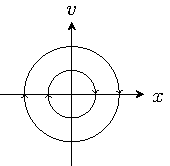
\includegraphics[width=0.8\columnwidth]{lezioni/tikz/lez_15_osc_armonico.pdf}
        \caption{\scriptsize Moto nello spazio delle fasi per un oscillatore armonico.}
        \label{fig:osc_armonico}
    \end{figure}
    %\begin{figure}[H]
    \centering
    \begin{tikzpicture}
	\begin{axis}[
	    width=4cm,
	    height=4cm,
	    xmin= -3, xmax= 3,
	    ymin= -3, ymax = 3,
	    axis lines = middle,
	    x label style={at={(axis description cs:1.1,0.56)},anchor=north},
	    y label style={at={(axis description cs:0.5,1)},anchor=south},
	    xlabel={$x$},
	    ylabel={$v$},
	    xtick={0},
	    ytick={0},
	    xticklabel={},
	    yticklabel={},
	    ]

	    \addplot [domain=-2:2, samples=100, ->] {sqrt(4-x^2)};
	    \addplot [domain=-2:2, samples=100, <-] {-sqrt(4-x^2)};

	    \addplot [domain=-1:1, samples=100, ->] {sqrt(1-x^2)};
	    \addplot [domain=-1:1, samples=100, <-] {-sqrt(1-x^2)};

	\end{axis}
    \end{tikzpicture}
    \caption{\scriptsize Moto nello spazio delle fasi per un oscillatore armonico.}
    \label{fig:osc_armonico}
\end{figure}

\end{exmp}
\noindent
\begin{exmp}[Pendolo]
    \[\begin{aligned}
	& \dot{x}=v\\
	& \dot{v}=-\frac{g}{l}\sin (x) 
    .\end{aligned}\]
    Dobbiamo prima cercare le traiettorie per il quale si annullano $\dot{x}$ oppure $\dot{v}$ (le nurk lines). 
    \begin{itemize}
        \item $\dot{x}$ si annulla quando $v = 0$, quindi per tale retta si ha una nurk line.
	\item $\dot{v}$ si annulla con $\sin (x) = 0$, quindi avremmo delle nurk line verticali per i seguenti valori di $x$: 
	    \[
		x = k\pi  \qquad k \in \mathbb{Z}
	    .\] 
    \end{itemize}
    Anche in questo caso è noto che vi è un integrale del moto (la cui derivata rispetto al tempo è nulla): 
    \[
	E = \frac{1}{2}v^2 - \frac{g}{l}\left(\cos (x) + 1\right)
    .\] 
    Quindi possiamo disegnare delle linee di flusso nello spazio delle fasi semplicemente plottando al variare di $E$  la seguente:
    \[
	v = \pm \sqrt{2 \left( E + \frac{g}{l}(1 + \cos (x)) \right) } 
    .\] 
    \begin{figure}[H]
        \centering
        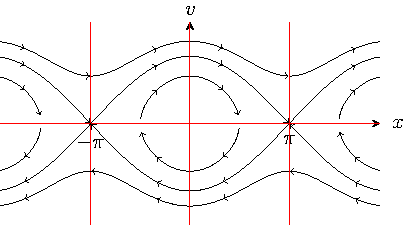
\includegraphics[width=0.8\columnwidth]{lezioni/tikz/lez_15_pendolo.pdf}
    \caption{\scriptsize Moto nello spazio delle fasi per il pendolo, le linee rosse indicano i valori di $x$ e $v$ per il quale si annullano la $\dot{v}$ o la $\dot{x}$. Le linee più esterne indicano un moto con $E > 0$, le linee che toccano l'asse $x$ e "rimbalzano" mantenendo il segno di $v$ sono quelle con $E = 0$ mentre le linee che girano nel centro dell'"occhio" hanno $E < 0$.}
    \label{fig:15_pendolo}
    \end{figure}
%    \documentclass[crop,tikz]{standalone}% 'crop' is the default for v1.0, before it was 'preview'
\usepackage{pgfplots}
\usetikzlibrary{math}
\begin{document}
    \begin{tikzpicture}
  	\tikzmath{\xa = 6; \y = 3;}
	\begin{axis}[
	    width=8cm,
	    height=5cm,
	    xmin= -\xa, xmax= \xa,
	    ymin= -\y, ymax = \y,
	    axis lines = middle,
	    x label style={at={(axis description cs:1.05,0.56)},anchor=north},
	    y label style={at={(axis description cs:0.5,1)},anchor=south},
	    xlabel={$x$},
	    ylabel={$v$},
	    xtick={0, pi, -pi},
	    xticklabels={$0$, $\pi$, $-\pi$},
	    ytick={0},
	    yticklabel={},
	    ]
	    %%%%%%%%%%%%%%%%%%%%%%%%%%%%%%%%%%%
	    %  Linea orizzontale (nurk line)  %
	    %%%%%%%%%%%%%%%%%%%%%%%%%%%%%%%%%%%
	    \addplot [domain=-\xa:\xa, samples=5, red] {0};
	    
	    \foreach \n in {-2*pi,0,2*pi} { % Vario "l'occhio" da visualizzare
		\foreach \s in {0.01,1,2} { % Traccio più linee per avere più punte di freccia
		    \foreach \E in {-1, 0 , 1} { % Vario l'energia per vedere le tre aree dello spazio delle fasi
			%%%%%%%%%%%%%%%%%%%%%%%%%%%%%%%%%%%%%%%%%%%%%
			%  Linee del moto al variare della energia  %
			%%%%%%%%%%%%%%%%%%%%%%%%%%%%%%%%%%%%%%%%%%%%%
		    	\addplot [domain= ( -pi-\n): ( pi-\n ) - 2*pi*\s/3, samples=100, ->] {sqrt( 2*(\E + 1 + cos(deg(x)) ))};
		    	\addplot [domain= ( -pi-\n) + 2*pi*\s/3: ( pi-\n ) , samples=100, <-] {-sqrt( 2*(\E + 1 + cos(deg(x)) ))};
		    }
		}
		%%%%%%%%%%%%%%%%%%%%%%%%%%%%%%%%%%
		%  Linee verticali (nurk lines)  %
		%%%%%%%%%%%%%%%%%%%%%%%%%%%%%%%%%%
	    	\addplot [red] coordinates {(\n/2, -\y) (\n/2, \y)};
	    }
	\end{axis}
    \end{tikzpicture}
\end{document}

    Notiamo in figura \ref{fig:15_pendolo} che nei punti 
    \[
        x = 2k\pi, \quad v = 0
    .\] 
    le linee di flusso si incrociano ma la dinamica del pendolo sembra presentare uno "spigolo": come se il moto rimbalzasse sull'asse $x$. Approfondiremo nel corso della lezione la natura di questi punti sella.
\end{exmp}
\noindent
In generale vale che:
\begin{redbox}{Linee di flusso nello spazio delle fasi}
    Dato un potenziale $U(x)$ possiamo disegnare delle linee di flusso ad energia fissata nello spazio delle fasi $v,x$ come:
    \[
	v = \pm \sqrt{2(E-U(x))} 
    .\] 
\end{redbox}
\noindent
\begin{exmp}[Moto in doppia buca]
Prendiamo un potenziale formato da una doppia buca asimmetrica, il moto nello spazio delle fasi è il seguente:    
\begin{figure}[H]
    \centering
    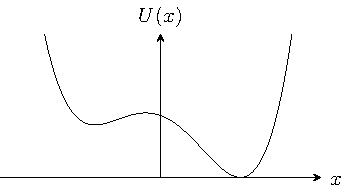
\includegraphics[width=0.8\columnwidth]{lezioni/tikz/lez_15_doppia_buca.pdf}
    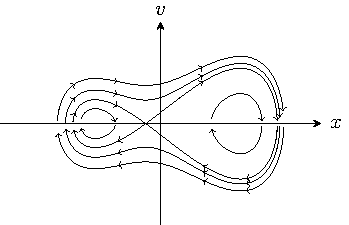
\includegraphics[width=0.8\columnwidth]{lezioni/tikz/lez_15_doppia_buca1.pdf}
    \caption{\scriptsize Potenziale a doppia buca e linee di flusso per il moto nello spazio delle fasi. Notiamo la presenza di un punto sella che equivale ad un moto nel quale l'oggetto raggiunge il punto di massimo tra le buche con velocità nulla (in un tempo infinito). }
    \label{fig:15_double}
\end{figure}
\noindent
%\begin{figure}[H]
    \centering
    \begin{tikzpicture}
  	\tikzmath{\xa = 2; \y = 3; \lim = 1.6;}
	\begin{axis}[
	    width=7cm,
	    height=4cm,
	    xmin= -\xa, xmax= \xa,
	    ymin= 0, ymax = \y,
	    axis lines = middle,
	    x label style={at={(axis description cs:1.05,0.06)},anchor=north},
	    y label style={at={(axis description cs:0.5,1)},anchor=south},
	    xlabel={$x$},
	    ylabel={$U(x)$ },
	    xtick={0},
	    xticklabels={$0$},
	    ytick={0},
	    yticklabel={$0$},
	    ]
	    \addplot[domain=-3:3, samples=500]{((x+1)^2+0.3)*(x-1)^2};
	\end{axis}
    \end{tikzpicture}
    \begin{tikzpicture}
  	\tikzmath{\xa = 2; \y = 3; \lim = 1.6;}
	\begin{axis}[
	    width=7cm,
	    height=5cm,
	    xmin= -\xa, xmax= \xa,
	    ymin= -\y, ymax = \y,
	    axis lines = middle,
	    x label style={at={(axis description cs:1.05,0.56)},anchor=north},
	    y label style={at={(axis description cs:0.5,1)},anchor=south},
	    xlabel={$x$},
	    ylabel={$v$},
	    xtick={0},
	    xticklabels={$0$},
	    ytick={0},
	    yticklabel={},
	    ]
	    \foreach \s in {0,1,2, 2.5} { % Traccio più linee per avere più punte di freccia
		\foreach \E in {1.354 , 1.6, 2} { % Vario l'energia per vedere le tre aree dello spazio delle fasi
		    %%%%%%%%%%%%%%%%%%%%%%%%%%%%%%%%%%%%%%%%%%%%%
		    %  Linee del moto al variare della energia  %
		    %%%%%%%%%%%%%%%%%%%%%%%%%%%%%%%%%%%%%%%%%%%%%
		    %((x+1)^2+0.5)*(x-1)^2
		    %(-x^2/2*(1-x^2/2) + 0.3)
		    \addplot [domain= ( -\lim): ( \lim) - 2*\lim*\s/3, samples=300, ->] {sqrt( 2*(\E - ((x+1)^2+0.3)*(x-1)^2)  )};
		    \addplot [domain= ( -\lim) + 2*\lim*\s/3: ( \lim) , samples=300, <-] {-sqrt( 2*(\E - ((x+1)^2+0.3)*(x-1)^2) )};
		}
	    }
	    \addplot [domain= ( 0): ( 1.9), samples=200, ->] {sqrt( 2*(0.4 - ((x+1)^2+0.3)*(x-1)^2)  )};
	    \addplot [domain= ( 0): ( 1.9) , samples=200, <-] {-sqrt( 2*(0.4 - ((x+1)^2+0.3)*(x-1)^2) )};
	    \addplot [domain= ( -1.9): ( 0), samples=200, ->] {sqrt( 2*(1.2 - ((x+1)^2+0.3)*(x-1)^2)  )};
	    \addplot [domain= ( -1.9): ( 0) , samples=200, <-] {-sqrt( 2*(1.2 - ((x+1)^2+0.3)*(x-1)^2) )};
	\end{axis}
    \end{tikzpicture}
    \caption{\scriptsize Potenziale a doppia buca e linee di flusso per il moto nello spazio delle fasi. Notiamo la presenza di un punto sella che equivale ad un moto nel quale l'oggetto raggiunge il punto di massimo tra le buche con velocità nulla (in un tempo infinito). }
    \label{fig:15_double}
\end{figure}

Notiamo in figura \ref{fig:15_double} che il moto può rimanere confinato all'interno di una delle due buche, esistono anche traiettorie che riescono ad entrare in tutte e due le buche "girando in tondo" nello spazio delle fasi. 
\end{exmp}
\noindent
In generale potremmo cercare un metodo per capire quali traiettorie scappano dal potenziale e quali invece rimangono confinate.
\subsection{Tecnica della stabilità lineare}%
\label{sub:Tecnica della stabilità lineare}
Prendiamo delle equazioni del moto del seguente tipo:
\[
    \begin{cases}
	\dot{x} = f(x, y) \\
	\dot{y} = g(x,y) 
    \end{cases}
.\] 
e supponiamo di aver identificato un punto $P_0=(x_0, y_0)$ tale per cui $\dot{x}=\dot{y}=0$.\\
La tecnica della stabilità lineare si basa sulla espansione delle equazioni del moto attorno al punto di equilibrio $P_0$.
\[\begin{aligned}
    & x = x_0 + \delta x\\
    & y = y_0 + \delta y
.\end{aligned}\]
Derivando queste due equazioni si ottiene: 
\[
    \begin{pmatrix} \delta\dot{x} \\ \delta\dot{y} \end{pmatrix} =
    \begin{pmatrix} 
	\partial_{x}f & \partial_{y}f\\
	\partial_{x}g & \partial_{y}g
    \end{pmatrix} 
    \begin{pmatrix} \delta x \\ \delta y \end{pmatrix} 
    \equiv 
    M 
    \begin{pmatrix} \delta x \\ \delta y \end{pmatrix} 
.\] 
A questo punto diagonalizzando la matrice $M$ si ottiene l'andamento del moto nello spazio delle fasi in un intorno del punto di stabilità $P_0$.
\[
    \text{det}\left|M-\lambda\mathbb{I}\right|=0
.\] 
Infatti ottenuto il set di $\lambda_i$ possiamo scrivere:
\[
    \delta \vect{x} = C_1\vect{D}_1e^{\lambda_1t} + C_2\vect{D}_2e^{\lambda_2t}
.\] 
Con $\vect{D}_i$ autovettori. Nel sistema di questi si ha che:
\[
    \dot{\vect{D}}  = \lambda  \vect{D}
.\] 
\subsection{Classificazione dei punti fissi}%
\label{sub:Classificazione dei punti fissi}
A seconda del segno degli autovalori possiamo riscontrare diverse situazioni:
\paragraph{Nodo stabile}%
\label{par:Nodo stabile}
Se gli autovalori sono entrambi negativi:
\[
    \lambda_1<\lambda_2<0
\] 
allora l'oggetto del moto cade nel punto $P_0$ esponenzialmente nel tempo (nello spazio degli autovettori $D_i$) come possiamo vedere in figura \ref{fig:figures-15_lambda-png}(a).
\paragraph{Nodo instabile}%
\label{par:Nodo instabile}
\[
    \lambda_1 > \lambda_2 > 0
.\] 
In questa situazione l'oggetto del moto si allontana esponenzialmente dal punto fisso (figura \ref{fig:figures-15_lambda-png}(b)).
\paragraph{Punto iperbolico}%
\label{par:Punto iperbolico}
\[
    \lambda_1<0<\lambda_2
.\] 
Questa è la situazione di punto sella accennato nel caso del pendolo (rappresentato figura \ref{fig:figures-15_lambda-png}(c), con le frecce rosse che so sovrappongono uscenti).
\paragraph{Spirale stabile/instabile}%
\label{par:Spirale stabile}
\[\begin{aligned}
    & \lambda_1 = -\alpha+i\beta\\
    & \lambda_2=-\alpha-i\beta
.\end{aligned}\]
In questo caso l'oggetto spiraleggia fino a cadere nel punto, in questi casi tale punto è spesso chiamato attrattore (figura \ref{fig:figures-15_lambda-png}(d)).\\
Nel caso della spirale instabile cambia soltanto il segno di $\alpha$:
\[\begin{aligned}
    & \lambda_1 = \alpha+i\beta\\
    & \lambda_2= \alpha-i\beta
.\end{aligned}\]
Gli oggetti si allontanano spiraleggiando dal punto in questione (figura \ref{fig:figures-15_lambda-png}(e))
\paragraph{Punto ellittico}%
\label{par:Punto ellittico}
\[\begin{aligned}
    & \lambda_1 = i\beta_1\\
    & \lambda_2= -i\beta_2
.\end{aligned}\]
In questo caso gli oggetti ruotano attorno al punto fisso, se $\beta_1=\beta_2$ allora la traiettoria nello spazio delle fasi è una circonferenza (figura \ref{fig:figures-15_lambda-png}(f)).
\begin{figure}[H]
    \centering
    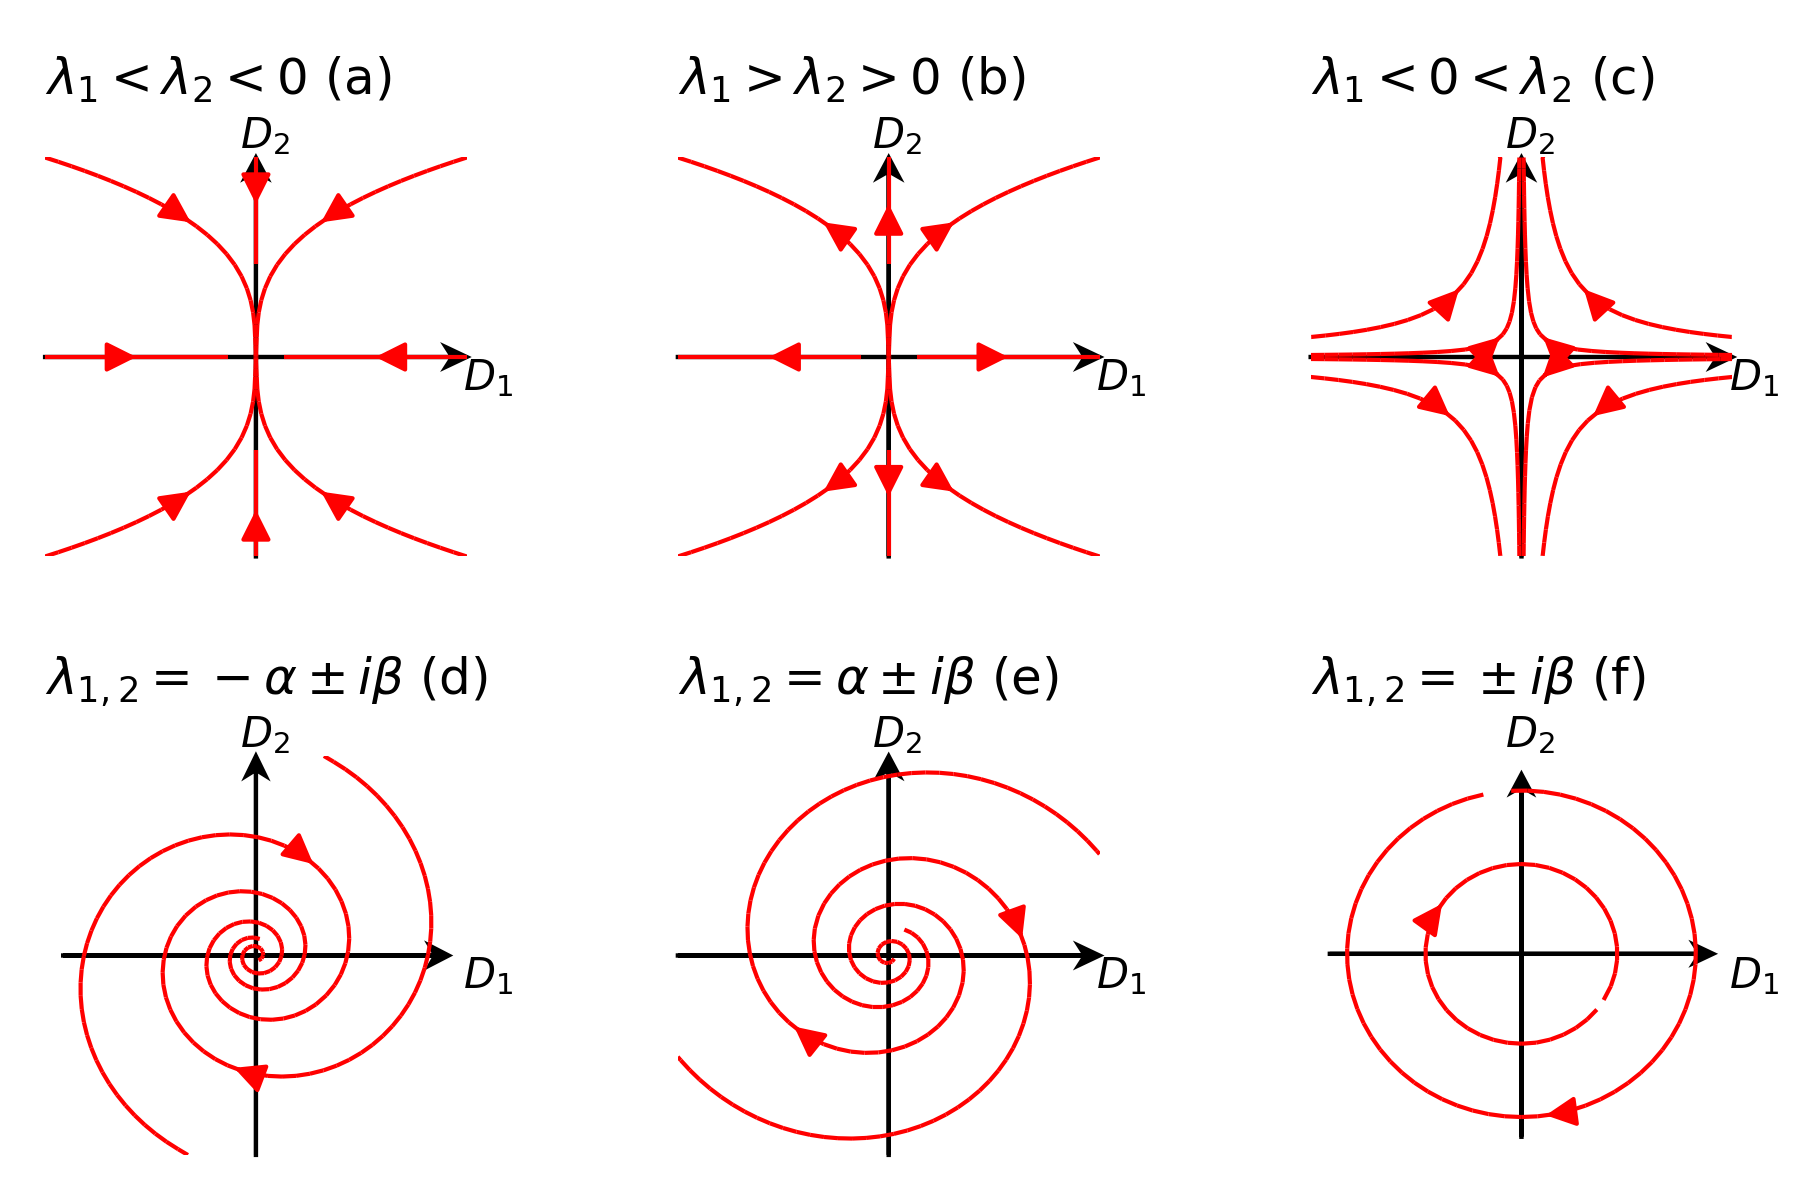
\includegraphics[width=0.5\textwidth]{figures/15_lambda.png}
    \caption{\scriptsize Classificazione dei punti fissi nello spazio delle fasi.}
    \label{fig:figures-15_lambda-png}
\end{figure}
\noindent
Un ultimo caso è dato dall'annullarsi di uno dei due autovalori, in tal caso il moto avviene lungo una retta nello spazio delle fasi.
\begin{exmp}[Osillatore smorzato]
    Prendiamo l'equazione del moto:
    \[
        \ddot{x}=-\omega_0^2x -\gamma\dot{x}
    .\] 
    Possiamo riscriverla nel seguente modo:
    \[
        \begin{cases}
 	    \dot{x} = v\\
	    \dot{v}=-\gamma v - \omega_0^2x           
        \end{cases}
    \] 
    L'unico punto di equilibrio per il sistema è $P_0 = (x_0 = 0, v_0 = 0)$.\\
    Possiamo cercare le Nurk line: 
    \[\begin{aligned}
	& \dot{x}=0 \implies  v = 0\\
	& \dot{v}=0 \implies  v = -\frac{\omega_0^2}{\gamma}x
    .\end{aligned}\]
    Abbiamo ottenuto due rette che dividono il piano in 4 parti. Sulla base di queste suddivisioni si potrebbe già indovinare come saranno le linee di flusso nello spazio delle fasi, è necessario infatti considerare che le Nurk lines corrispondono ad una variazione di segno di $\dot{x}, \dot{v}$, quindi ci indicano la direzione dell'oggetto nello spazio delle fasi.\\
    Graficando le linee e osservando la direzione degli oggetti nel piano potremmo già concludere che i corpi spiraleggiano attorno all'origine. Proviamo a vederlo con il metodo descritto in questa sezione.
    \[
	\begin{pmatrix} \delta\dot{x} \\ \delta\dot{v} \end{pmatrix} =
	\begin{pmatrix} 
	    0 & 1\\
	    -\omega_0^2 & - \gamma
	\end{pmatrix} 
	\begin{pmatrix} \delta x \\ \delta y \end{pmatrix} 
    .\] 
    \[
        \lambda  = \frac{-\gamma  \pm \sqrt{\gamma^2 - 4\omega_0^2}}{2}
    .\] 
    Quindi possiamo distinguere due situazioni:
    \begin{itemize}
        \item  $\gamma^2 - 4\omega_0^2 > 0$. \\
	In questo caso gli autovalori $\lambda_1, \lambda_2$ sono entrambi reali, quindi l'origine è un nodo stabile.
    \item $\gamma^2 - 4\omega_0^2 < 0$.\\
	In tal caso si ha che:
	\[
	    \lambda_{1,2} = -\frac{\gamma}{2} \pm i \omega
	.\] 
	Quindi in tal caso l'origine è un punto di spirale stabile.
    \end{itemize}
    Notiamo che in questo caso particolare, poiché la matrice delle derivate miste perde la dipendenza da $v$ e $x$, lo sviluppo lineare vale in tutto il piano e non soltanto in un intorno dell'origine.
\end{exmp}
\noindent
\begin{exmp}[Pendolo smorzato]
    L'equazione per il pendolo smorzato è:
    \[
        \begin{cases}
            \dot{x} = v\\
	    \dot{v} = - g /l\sin (x) - \gamma v
        \end{cases}
    \] 
    I nodi stabili sono tutti i punti tali che:
    \[\begin{aligned}
	& v_0 = 0\\
	& x_0 = n \pi
    .\end{aligned}\]
    Prendendo la matrice delle derivate miste si ha:
    \[\begin{aligned}
	\begin{pmatrix} \delta\dot{x} \\ \delta  \dot{v} \end{pmatrix} =&
	\left.	\begin{pmatrix} 
	    0 & 1 \\
	    -g /l \cos (x) & - \gamma
	\end{pmatrix} \right|_{x_0,y_0}
	\begin{pmatrix} \delta x \\ \delta v \end{pmatrix} \\
	=&
	\begin{pmatrix} 
	    0 & 1 \\
	    \pm g /l& - \gamma
	\end{pmatrix}
	\begin{pmatrix} \delta x \\ \delta v \end{pmatrix} 
    .\end{aligned}\]
    Gli autovalori del sistema sono quindi:
    \[
        \lambda  = \frac{-\gamma}{2}\pm \sqrt{\frac{\gamma^2}{4} \pm \frac{g}{4l}} 
    .\] 
    Si hanno quindi due situazioni distinte a seconda del segno presente nella radice degli autovalori:
    \begin{itemize}
	\item \textbf{Segno $+$}: ($x_0 = (2n+1)\pi$):\\
	    $\lambda_1 < 0,  \lambda_2 > 0 \implies$ Punto sella.
	\item \textbf{Segno $-$}: ($x = 2n\pi$): 
	    \begin{itemize}
		\item $\gamma^2 / 4 > g /(4l)$: \\
		    $\lambda_1,\lambda_2 < 0 \implies$ Nodo stabile.
		\item $\gamma^2 / 4 < g /(4l)$: \\
		    $\lambda_{1,2} $ C.C. $\implies$ Spirale stabile.
	    \end{itemize}
    \end{itemize}
    \begin{figure}[H]
        \centering
	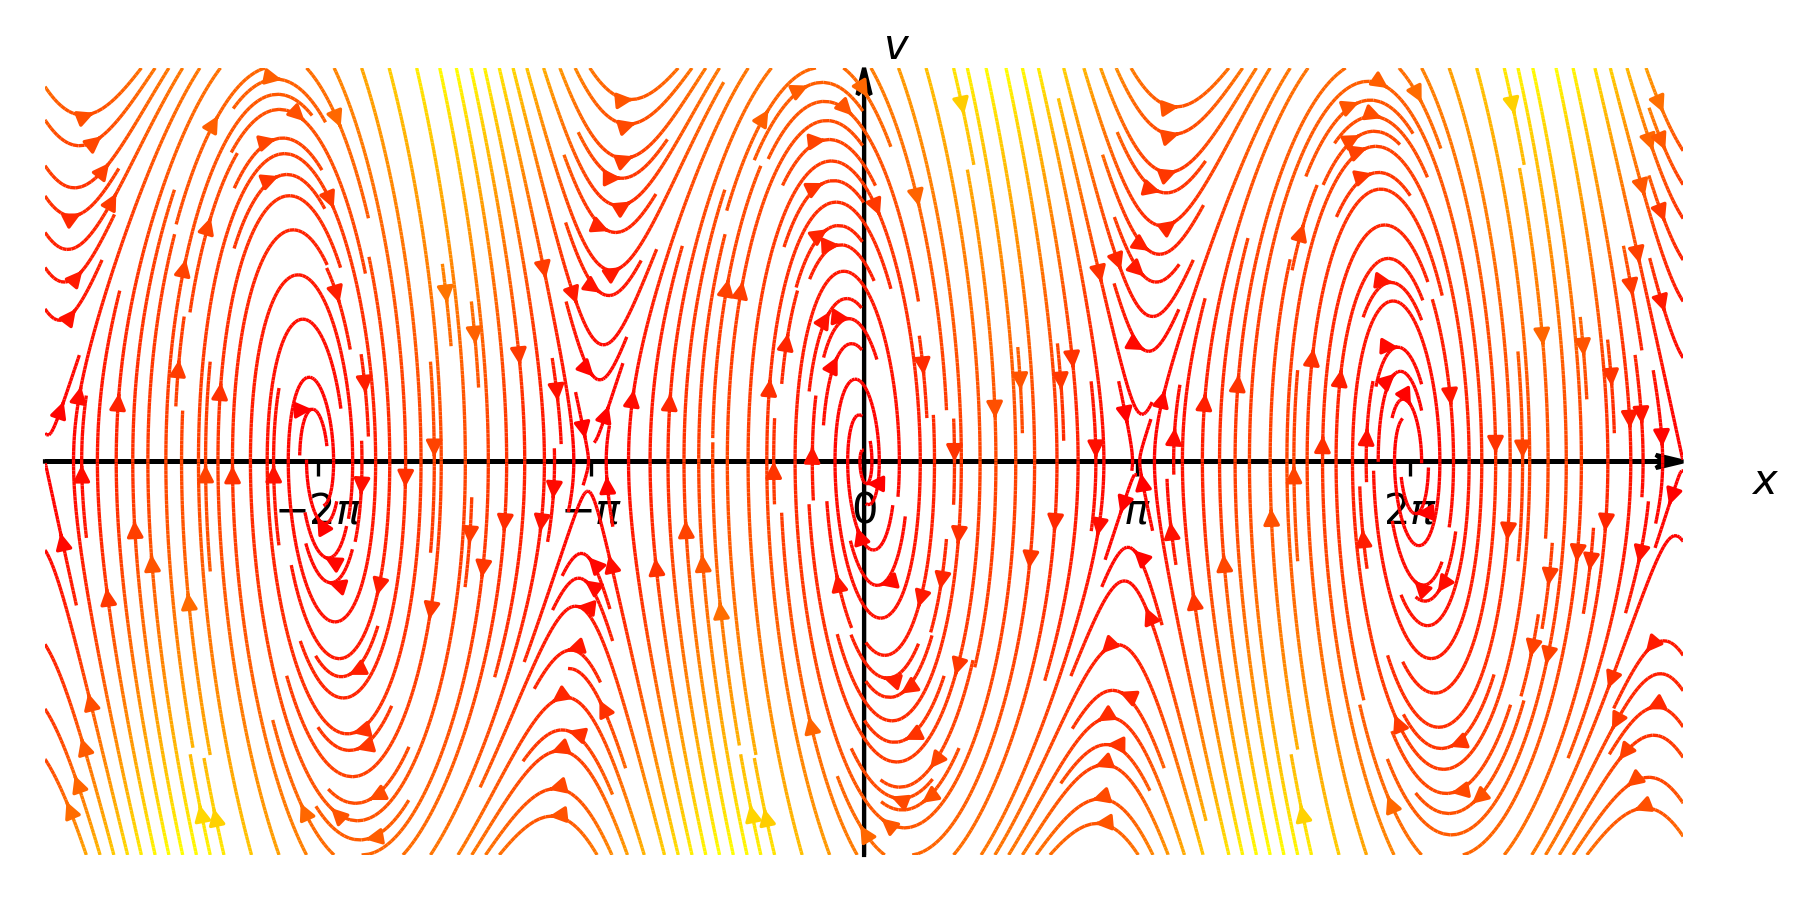
\includegraphics[width=0.5\textwidth]{figures/15_pendolo.png}
	\caption{\scriptsize Rappresentazione del pendolo smorzato nello spazio delle fasi, grossolanamente si riescono a distinguere le spirali ed i punti sella. I colori indicano la "velocità" nello spazio delle fasi ($\sqrt{\dot{x}^2+\dot{v}^2}$), il giallo indica zone con tale quantità minore, il rosso le zone in cui gli oggetti si muovono più "velocemente".}
        \label{fig:fig}
    \end{figure}
    Interessante notare come viene "rotta" la spirale all'aumentare del parametro $\gamma$:
    \begin{figure}[H]
        \centering
	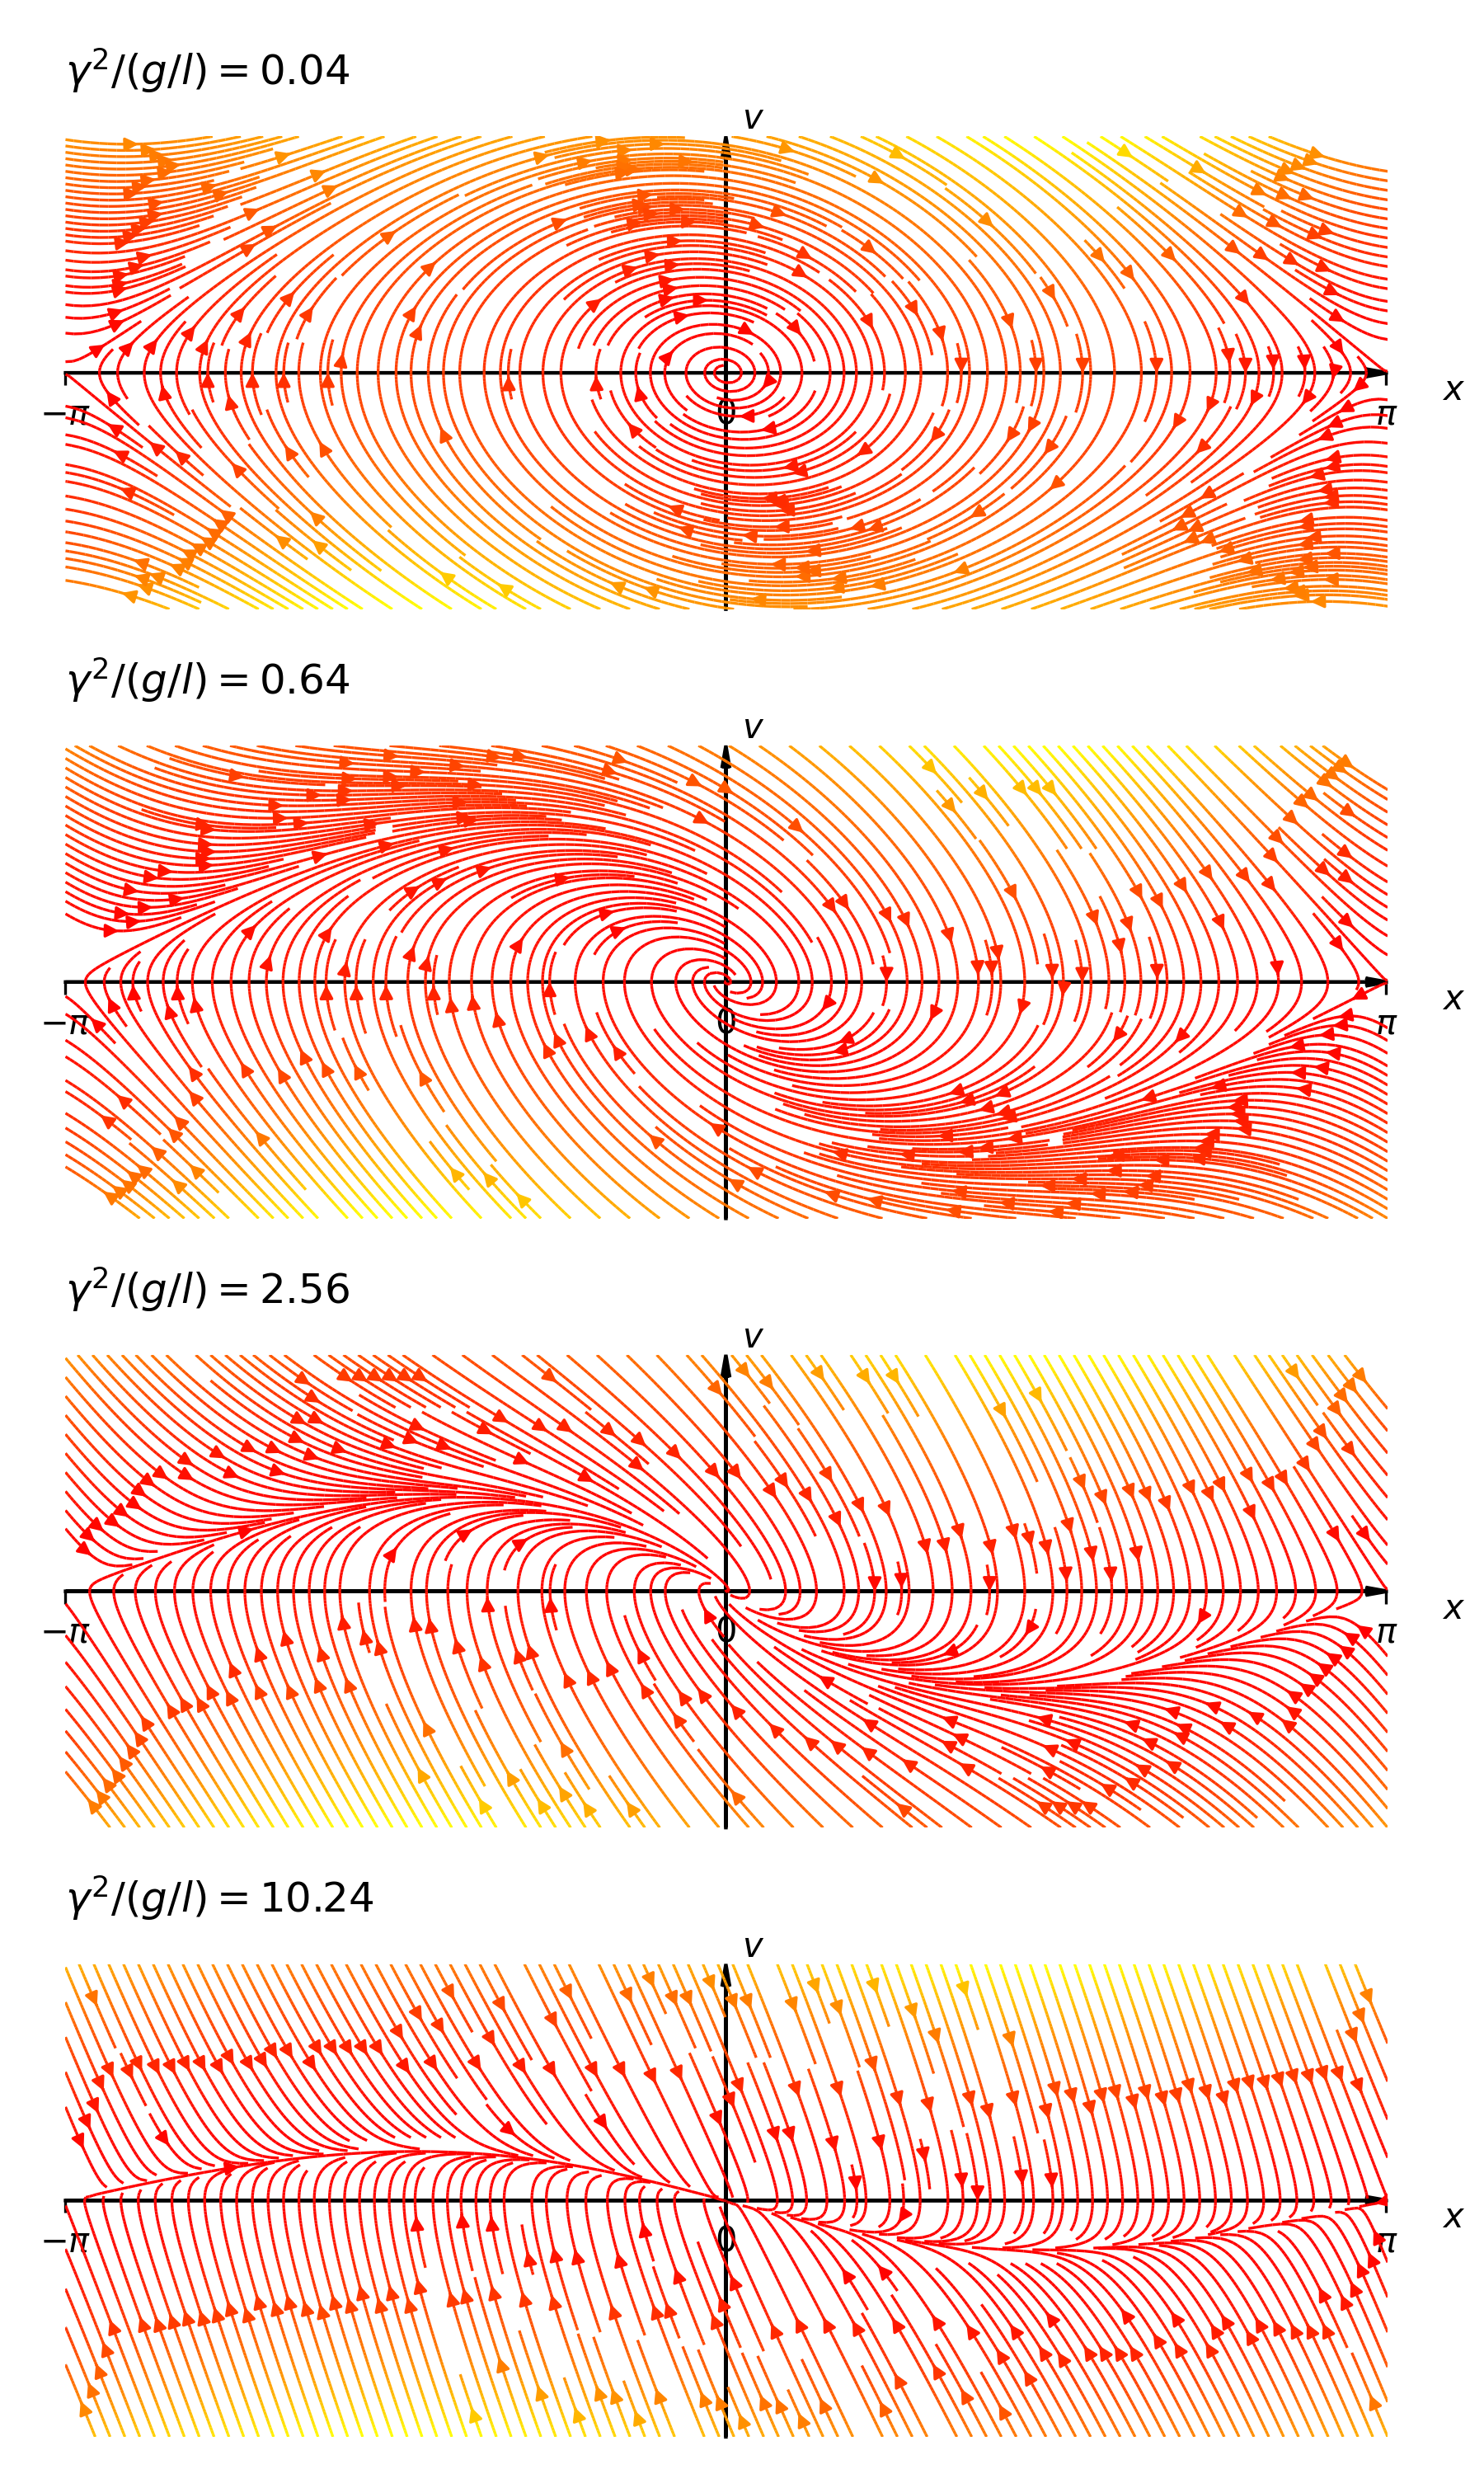
\includegraphics[width=0.5\textwidth]{figures/15_pendolo_accartoccio.png}
	\caption{\scriptsize Forma del flusso attorno all'origine al variare del rapporto $\gamma  / (g /l)$, si nota come la spirale sparisca all'aumentare di $\gamma$. Le linee di flusso tendono a collassare in modo anticipato su una curva oscillante.}
        \label{fig:figures-15_pendolo_accartoccio-png}
    \end{figure}
\end{exmp}
\noindent
\begin{exmp}[Equazioni di Lotka-Volterra]
    \[
        \begin{cases}
	    \dot{x} = x - xy\\
	    \dot{y} = - y + xy
        \end{cases}
    \] 
    In cui $x, y > 0$. \\
    I punti stazionari per queste equazioni sono (quando si annullano sia $\dot{x}$ che $\dot{y}$):
    \[\begin{aligned}
	& P_0 = (0,0) \\
	& P_1 = (1,1) 
    .\end{aligned}\]
    Le nurk lines invece sono le quattro rette:
    \[\begin{aligned}
        x = 0 \qquad x = 1\\
	y = 0 \qquad y = 1
    .\end{aligned}\]
    Passiamo direttamente al sistema linearizzato:
    \[
        \begin{pmatrix} \delta\dot{x} \\ \delta\dot{y} \end{pmatrix} =
	\begin{pmatrix} 
	  1-y & -x \\
          y & -1+x
        \end{pmatrix} 
	\begin{pmatrix} \delta x \\ \delta y \end{pmatrix} 
    .\] 
    Si tratta adesso di valutare i due punti fissi singolarmente per vedere di che tipo sono.\\
    Per l'origine degli assi si ha che la matrice $M$ è:
    \[
	M_{00} = 
        \begin{pmatrix} 
	1 & 0\\
        0 & -1
        \end{pmatrix} 
    .\] 
    La matrice è già in forma diagonale, quindi si ha un autovalore positivo ed uno negativo: l'origine è un punto iperbolico.\\
    Per quanto riguarda il punto $x=y=1$ si ha
    \[
	M_{11} = 
        \begin{pmatrix} 
	0 & -1\\
        1 & 0
        \end{pmatrix} 
    .\] 
    gli autovalori sono $\pm i$, quindi il punto è ellittico.
    \begin{figure}[H]
        \centering
	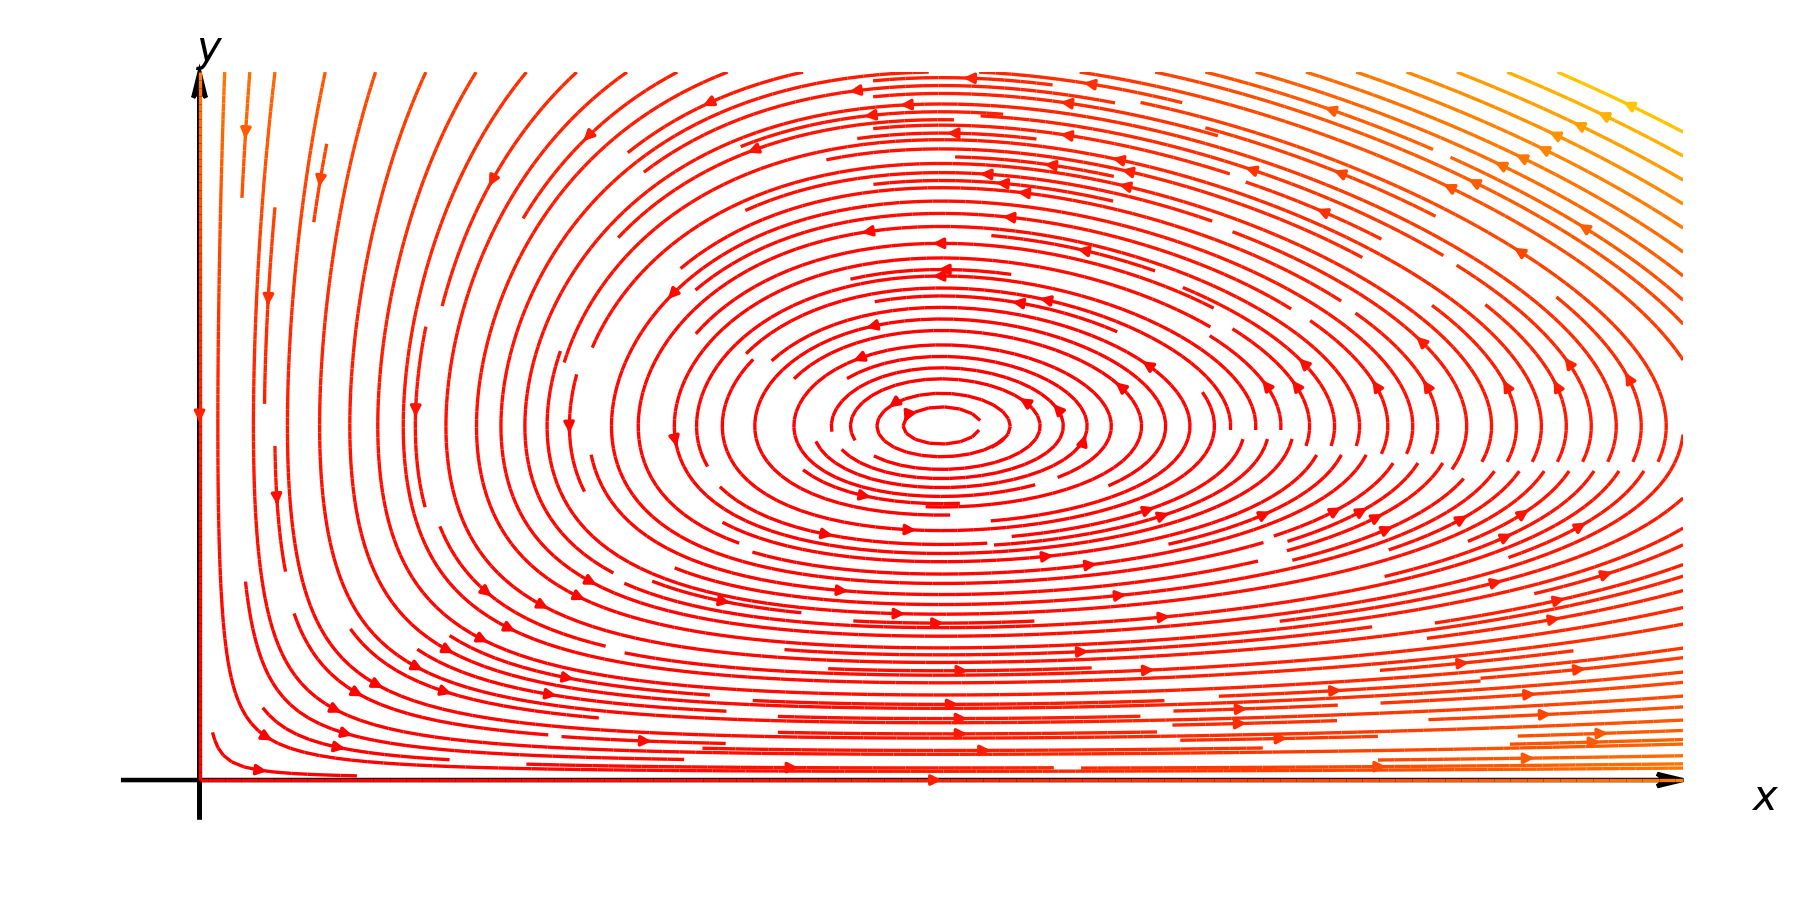
\includegraphics[width=0.5\textwidth]{figures/15_volterra.png}
        \caption{\scriptsize Flusso nello spazio delle fasi per il sistema di Lotka-Volterra.}
        \label{fig:figures-15_volterra-png}
    \end{figure}
    Questa equazione è studiata nel contesto della dinamica delle popolazioni, come già accennato nella primissima lezione.
\end{exmp}
\noindent
\begin{exmp}[Equazione non lineare incasinata]
    Prendiamo il sistema di equazioni:
    \[
        \begin{cases}
	    \dot{x} = x + y - x (x^2+y^2) \\
	    \dot{y}=- x + y - y(x^2+ y^2) 
        \end{cases}
    .\] 
    Non è chiaro dalle equazioni se vi è un punto fisso, una strategia vincente di soluzione è cambiare variabile.
    \[
        R^2=x^2+y^2
    .\] 
    Così facendo si ha che:
    \[
        \frac{\text{d} R^2}{\text{d} t} = R^2-R^4
    .\] 
    Con l'ulteriore cambio di variabili $R^2 = z$ si ottiene l'equazione semplificata:
    \[
        \dot{z}=z-z^2
    \] 
    che presenta i seguenti punti fissi:
    \[\begin{aligned}
	& z = 0\\
	& z = 1
    .\end{aligned}\] 
    Valutare gli autovalori è più semplice in una dimensione:
    \[
	\delta\dot{z}=(1-2z) \delta z
    .\] 
    Nel caso di $z=0$ si ha $\lambda =1$: punto instabile. Nel caso di $z=1$ si ha $\lambda =-1$: punto stabile.\\
    La grossa differenza dai sistemi visti in precedenza è che il punto $z=1$ è in realtà una varietà stabile nel sistema di coordinate di partenza $x^2+y^2=1$.
    Tutti i punti del piano $x,y$ tenderanno a cadere sulla circonferenza di raggio unitario. 
\end{exmp}
\noindent
\clearpage

\section{Lezione 16}%
\label{sub:Lezione 16}
\subsection{Trasformazioni canoniche}%
\label{sub:Trasformazioni canoniche}
\begin{redbox}{}
    Una trasformazione canonica è un cambio di variabili generalizzate tale che:
    \[
        H(p_i, q_i) = H'(P_i(p_i,q_i), Q_i(p_i, q_i) ) 
    .\] 
    Le nuove variabili devono rispettare le regole di commutazione canoniche:
    \[
	\dot{Q}_i = - \left[ Q_i,H\right] \qquad \dot{P}_i = \left[P_i, H\right]
    .\] 
\end{redbox}
\noindent
Spesso nello studio dei sistemi Hamiltoninani è necessario trovare delle trasformazioni che permettano di integrare H. \\
Integrare l'Hamiltoniana significa trovare le $P_i, Q_i$  tali che:
\[
    H(p_i, q_i) \to H'(P_i) 
.\] 
Quindi per le equazioni di Hamilton-Jacoby anche:
\[\begin{aligned}
    & \dot{P}_i = - \frac{\partial H'}{\partial Q_i} =0\\
    & \dot{Q}_i = \frac{\partial H'}{\partial P_i} = f_i(P_i) 
.\end{aligned}\]
Questo ci permette di trovare una equazione del moto come:
\[
    \dot{Q}_i = f_i(P_i) t + Q_i(0) 
.\] 
Per ottenere una trasformazione canonica è necessario passare dalle \textbf{Funzioni generatrici}.\\
Per trovare queste funzioni partiamo dalla considerazione che $H$ conserva il volume nello spazio delle fasi, quindi anche $H'$ deve conservare tale volume:
\[
    \int\int dpdq = \int\int dPdQ
.\] 
Quindi possiamo sfruttare il teorema di stokes:
\[
    \oint pdq = \oint  QdP
.\] 
\begin{equation}
    \oint  \left[pdq - QdP\right] = 0 
    \label{eq:16_stokes}
\end{equation}
Grazie a questo integrale possiamo riscrivere tutto in funzione di $q$ e $P$.\\
La quantità nell'integrale di linea \ref{eq:16_stokes} è il differenziale di una qualche funzione $F_2$:
\[
    \oint dF_2(q,P) = \oint \frac{\partial F_2}{\partial q} dq + \frac{\partial F_2}{\partial P} dP = 0 
.\] 
Quindi:
\[\begin{aligned}
    &p = \partial_{q}F_2(q,P) \\
    &Q = - \partial_{P}F_2(q,P) 
.\end{aligned}\]
Notiamo che aver scritto tutto in funzione della coppia $(q,P)$ è una scelta (che conduce al funzionale chiamato storicamente $F_2$), si potevano effettuare altre scelte ottenendo lo stesso formalismo con funzionali dipendenti dalle coppie scelte.\\
Quello che interessa a noi è trovare la trasformazione furba che ci permetta di integrare l'Hamiltoniana.
\subsection{Ricerca della trasformazione che integra $H$}%
\label{sub:Ricerca della trasformazione per integrare H}
Supponiamo che la trasformazione ideale sia $S(\vect{q}, \vect{\alpha})$, con $\vect{\alpha}$ nuovi momenti conservati (quelli che prima erano $P$). Analogamente definiamo le $Q$ ideali per la trasformazione come $\beta$.\\
Esplicitiamo le equazioni del cambio di vaiabili in questo caso:
\[
    p_i = \frac{\partial S}{\partial q_i} \qquad \beta_i = - \frac{\partial S}{\partial \alpha_i} 
.\] 
Esplicitando queste trasformazioni nella dipendenza da $p_i$ di $H$ si ottiene:
\[
    H(\vect{q}, \frac{\partial S}{\partial \vect{q}}) = H'(\vect{\alpha}) 
.\] 
Quindi questa equazione ci permette di esprimere delle Equazioni di HJ, tramite tali equazioni possiamo invertire e trovare $\partial_{q}S$, infine di integra per trovare la $S$ ideale.\\
In generale risolvere il problema è molto complicato, per semplificare il calcolo dobbiamo considerare il fatto che gli $\vect{\alpha}$ sono delle costanti del moto
\footnote{Per definizione della trasformazione che cerchiamo si ha che $\dot{\alpha}_i = -\partial_{\beta}H' = 0$ }
. Tenendo conto di questo il differenziale della derivata di $S$ ($dS'$) si esprime come:
\[
    dS' = \sum_{}^{} \frac{\partial S}{\partial q_i} dq_i = \sum_{}^{} P_idq_i
.\] 
ed integrando si ha direttamente:
\[
    S = \int_{q_0}^{q_t} \sum_{i}^{} P_idq_i 
.\] 
\begin{exmp}[Hamiltoniana 1D]
    Prendiamo una trasformazione nello spazio unidimensionale tale che:
    \[
	H(q,\partial_{q}S) = H'(\alpha) = \alpha
    .\] 
    Le coordinate dipendenti possono essere espresse tramite la trasformazione (ignota) come:
    \[\begin{aligned}
	& p = \partial_{q}S(q, \alpha) \\
	& \beta  = \partial_{\alpha}S(q, \alpha) 
    .\end{aligned}\]
    Le equazioni HJ sono:
    \[\begin{aligned}
	&\dot{\alpha}= - \partial_{\beta} H' = 0\\
	&\dot{\beta} = \partial_{\alpha}H' = 1
    .\end{aligned}\]
    Possiamo integrare quindi per $\beta$ (imponiamo che $\beta (t=0) =0$):
    \[
        \beta  = t-t_0
    .\] 
    Quindi abbiamo che:
    \[\begin{aligned}
	t-t_0 =& \int dt \dot{\beta} 
	       = \int_{q_0}^{q_t} d\beta (q) \\
	       & = \int_{q_0}^{q_t} \partial_{q}\beta dq 
	       = \int  \partial_{q}\partial_{\alpha}S dq = \\
	       & = \int\partial_{\alpha }\partial_{q}Sdq
	       = \int_{q_0}^{q_t} \partial_{\alpha}P(q, \alpha) dq 
    .\end{aligned}\]
    In definitiva possiamo scrivere il $t-t_0$ in funzione di quell'ultimo integrale:
    \[
        t-t_0 = \int_{q_0}^{q_t} \partial_{\alpha}P(q, \alpha) dq 
    .\] 
\end{exmp}
\noindent
\begin{exmp}[Moto in potenziale a energia fissa]
    Prendiamo l'Hamiltoniana unidimensionale con un potenziale:
    \[
	H = \frac{p^2}{2} + V(q) = \alpha
    .\] 
    In questo caso il nuovo momento della trasformazione è l'energia del sistema.\\
    Esplicitiamo $P(q,\alpha)$ in funzione delle variabili selezionate:
    \[
	P(q,\alpha) = \sqrt{2(\alpha-V(q))} 
    .\] 
    Quindi otteniamo un tempo $t-t_0$ che rappresenta il periodo del moto:
    \[
	t-t_0 = \int_{q_0}^{q_t} \frac{1}{\sqrt{2(\alpha-V(q))}}dq 
    .\] 
\end{exmp}
\noindent
\begin{exmp}[Moto in campo centrale]
    \[
	H = \frac{p^2_r}{2} + \frac{p_\phi^2}{2r^2} + V(r) 
    .\] 
    In questo caso abbiamo un momento conservato: $p_\phi$, quindi abbiamo una quantità per il moto $\alpha_\phi$ che si conserva. Possiamo scrivere in tal caso:
    \[
	S(\vect{q}, \vect{\alpha}) = \alpha_\phi\phi  + S_1(r, \alpha_1) 
    .\] 
    In questo modo sappiamo che derivando rispetto a $\phi$  si ottiene la quantità conservata.\\
    Riscriviamo l'Hamiltoniana:
    \[
	H' = \frac{1}{2}\left[(\partial_{r}S_1)^2 + \frac{\alpha_\phi^2}{r^2}\right] + V(r) = \alpha_1
    .\] 
    Scriviamo l'equazione per l'incognita: $\partial_{r}S_1$:
    \[
	\partial_{r}S_1 = \sqrt{2\left[\alpha_1 - V(r) \right]- \frac{\alpha_\phi^2}{r^2}} 
    .\] 
    Questa equazione può essere integrata, si ottiene immediatamente che:
    \[
        S = \alpha_\phi\phi  + \int dr \sqrt{2\left[\alpha_1 - V(r) \right]- \frac{\alpha_\phi^2}{r^2}} 
    .\] 
    A questo punto si fanno i passaggi dell'esempio precedente (c'è un cambio di notazione: $-t_0\to \beta_1$), quindi si ha:
    \[
	\beta_1 + t = \frac{\partial S}{\partial \alpha_1} = \int  \frac{dr}{\sqrt{2(\alpha_1-V(r))- \alpha^2_\phi  /r^2}}
    .\] 
    \[
	\beta_2 = \frac{\partial S}{\partial \alpha_\phi} = \int  \frac{d\phi}{\sqrt{2(\alpha_1-V(r))- \alpha^2_\phi  /r^2}} + \phi
    .\] 
    Notiamo che non aver inserito la dipendenza dal tempo per $\beta_2$ è una conseguenza di tutto il meccanismo utilizzato: deriva direttamente dalle equazioni d Hamilton:
    \[
        H' = \alpha_1 \implies  \frac{\partial H'}{\partial \alpha_\phi} = 0 = \dot{\beta_2}
    .\] 
\end{exmp}
\noindent
\subsection{Variabili azione-angolo in una dimensione}%
\label{sub:Variabili azione-angolo}
Partiamo con la seguente:
\begin{redbox}{}
    Per Hamiltoniane limitate in 1D il moto nello spazio delle fasi avviene sempre su traiettorie chiuse.
\end{redbox}
\noindent
Di conseguenza potremmo cercare una variabile angolo $\theta$ che aumenti di $2\pi$ dopo un giro. Definiamo il momento coniugato di questa variabile come $I$
\footnote{Il motivo per il quale storicamente è di interesse proprio questa trasformazione è che venne studiata per valutare la stabilità del sistema solare}.\\
La trasformazione canonica cercata è $S(q, I)$.
\[
    p = \partial_{q}S(q,I) \qquad \theta  = \partial_{I}S(q,I) 
.\] 
Inoltre dobbiamo fare in modo che la trasformazione permetta di integrare l'Hamiltoniana, serve quindi che:
\[
    H(q, \partial_{q}S) = \alpha  = H'(I) 
.\] 
Il fatto che la variabile $\theta$ sia periodica porta con se il vantaggio di poter fare teoria delle perturbazioni, come approfondiremo nella prossima lezione.\\
Procediamo supponendo $\alpha$ costante e fissato. 
\[
    \partial_{q}\theta  = \partial_{q}\partial_{I}S = \partial_{I}\partial_{q}S \ ( = \partial_{I}P(I) ) 
.\] 
Visto che dopo un giro si ha che: $\theta\to \theta +2\pi$.
\[
    2\pi  = \oint _c d\theta  = \frac{\partial }{\partial I} \oint \frac{\partial S}{\partial q} dq = \frac{\partial }{\partial I} \oint p dq 
.\] 
Questo implica un importante teorema:
\begin{redbox}{}
    \[
        \oint pdq = 2\pi I 
    .\] 
    quindi abbiamo una azione (fissata una curva chiusa nello spazio delle fasi):
    \[
        I = \frac{1}{2\pi}\oint_c pdq 
    .\] 
\end{redbox}
\noindent
Operativamente quello che si fa per risolvere è:
\begin{itemize}
    \item Si risolve l'Hamiltoniana nel cambio di variabili:
	\[
	    H(q,\partial_{q}S) = \alpha
	.\] 
    \item Si calcola l'azione $I$ con la formula sopra sulle curve $c$ che hanno $\alpha$ costante.
\end{itemize}
Le equazioni canoniche per le nuove variabili $I,\theta$ sono:
\begin{redbox}{}
\[
    \dot{I}=-\partial_{\theta  }H'(I) = 0 \qquad \dot{\theta} = \partial_{I}H'(I) = \omega (I) 
.\]    
\end{redbox}
\noindent
Visto che la $I$  è costante nel tempo integriamo l'equazione per $\dot{\theta}$  ottenendo:
\[
    \theta (t) = \omega (I) t + \theta_0
.\] 
La cosa importante è che tutta la fisica del problema è inclusa nella dipendenza di $\omega$  dall'azione $I$.
\begin{exmp}[Oscillatore armonico]
    Prendiamo l'equazione per un oscillatore armonico unidimensionale:
    \[
        H = \frac{p^2}{2} + \frac{\omega^2_0 q^2}{2}
    .\] 
    Abbiamo come sempre che
    \[
        p = \frac{\partial S}{\partial q} 
    .\] 
    Quindi l'Hamiltoniana si esprime come:
    \[
        \frac{1}{2}\left(\frac{\partial S}{\partial q} \right)^2 + \frac{1}{2} \omega_0^2q^2 = \alpha
    .\] 
    Passiamo direttamente alla ricerca della azione $I$:
    \[
	I = \frac{1}{2\pi}\oint pdq = \frac{1}{2\pi}\oint _c \sqrt{2(\alpha-\frac{1}{2}\omega_0^2q^2) }dq = \frac{\alpha}{\omega_0}
    .\] 
    Possiamo trovare anche il periodo del moto e sfruttarlo per valutare la $I$:
    \[
        T = \oint _c\left(\frac{\partial }{\partial \alpha} p\right)dq = \frac{\partial }{\partial \alpha} \oint _cpdq = \frac{\partial }{\partial \alpha} 2\pi I  
    .\] 
    Abbiamo quindi:
    \[
        I = \frac{T}{2\pi}\alpha  = \frac{\alpha}{\omega_0}
    .\] 
    In conclusione abbiamo ad esempio:
    \[
        \alpha  = \omega_0I = H'
    .\] 
    In generale ci si aspetta una Hamiltoniana trasformata del tipo:
    \[
	H' = \omega (I) I
    .\] 
    Possiamo esplicitare anche la trasformazione $S$  in modo da ottenere delle equazioni per il moto:
    \[
	S(q,I) = \int\sqrt{2(\omega_0I- \frac{\omega_0^2q^2}{2})} dq
    .\] 
    Per tornare indietro ed ottenere $q(t)$ è necessario fare un bel calcolo, bisogna tornare indietro passando per la definizione di $\theta  $:
    \[
	\theta = \partial_{I}S(I,q) 
    .\] 
    Quindi derivando all'interno dell'integrale si ottiene:
    \[
	\theta  = \sqrt{\frac{2\omega_0}{I}} \int dq \frac{1}{\sqrt{1-\frac{\omega_0}{2I} q^2}}
    .\] 
    Oltre ad effettuare la derivata si è raccolto un termine per esplicitare l'integrale, l'integrale può essere risolto con un cambio di variabili trigonometrico e conduce all'inverso del seno:
    \[
	\theta  = \sqrt{\frac{2\omega_0}{I}} \frac{\sin^{-1}(\sqrt{\frac{\omega_0}{2I}} q)}{\sqrt{\frac{2\omega_0}{I}} } + c
    .\] 
    Se ne conclude che:
    \begin{equation}
        \begin{cases}
	    q = \sqrt{2I /\omega_0} \sin (\theta  + \delta_0) \\
	    \theta  = \omega_0t
        \end{cases}
	\label{eq:16_q}
    \end{equation}
\end{exmp}
\noindent
\subsection{Variabili azione-angolo in dimensioni $D\ge 2$.}%
\label{sub:Variabili azione angolo in dimensioni >2.}
Nel caso di Hamiltoninane separabili il problema si risolve in modo semplice: basta trovare $n$ costanti dell moto (in $n$ dimensioni).\\
Se si trovano tali costanti allora il moto è confinato ad una varietà $n$ dimensionale nello spazio delle fasi ($2n$ dimensionale).
\begin{redbox}{Teorema di Poincare}
    Data una Hamiltoniana $n$ dimensionale a variabili separabili.\\
    Consideriamo la trasformazione canonica che integra l'Hamiltoniana, la varietà su cui giacciono le traiettorie è un \textbf{Toro} ($M$) $n$-dimensionale.
\begin{figure}[H]
    \centering
    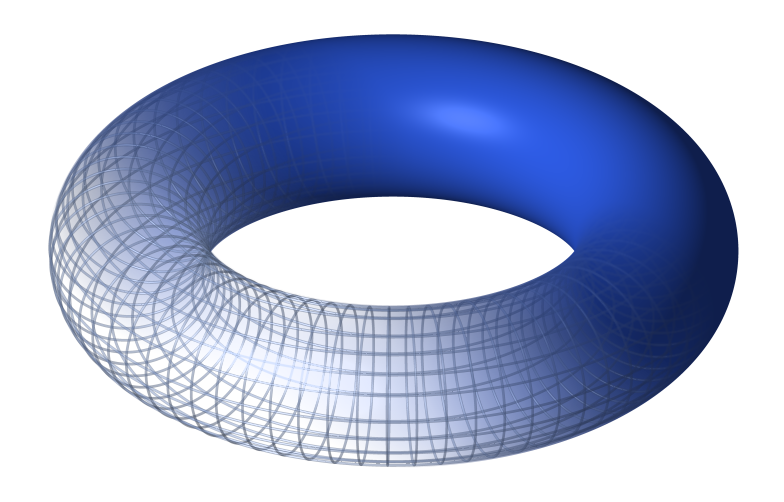
\includegraphics[width=0.8\textwidth]{figures/lez_16_Torus_low_quality.png}
    \caption{\scriptsize Toro in 3 dimensioni, ricordiamo che generalmente si parla di toro $n$ dimensionale.}
    \label{fig:figures-lez_16_Torus_low_quality-png}
\end{figure}
\noindent
\end{redbox}
\noindent
La dimostrazione è complicata, possiamo immaginarla visivamente pensando che il toro è l'unica varietà che, se considerata letteralmente pelosa, può essere pettinata. Una qualunque altra varietà, come una sfera ad esempio, presenterà delle stizze durante la pettinatura.
\begin{figure}[H]
    \centering
    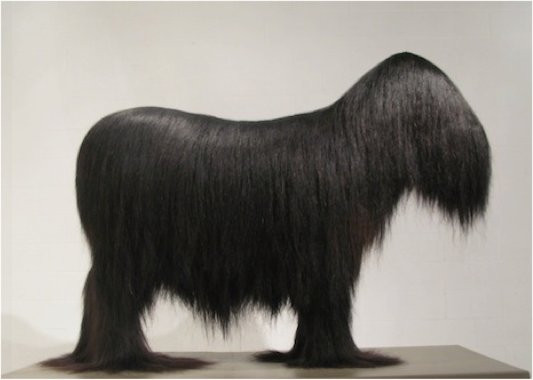
\includegraphics[width=0.4\textwidth]{figures/lez_15_toro_peloso.jpg}
    \caption{\scriptsize Un toro perfettamente pettinato}
    \label{fig:figures-lez_15_toro_peloso-jpg}
\end{figure}
\noindent
Formalmente se $\dot{\xi}$ è il campo di "velocità" che descrive il flusso di $H$ su $M$ il toro è l'unica varietà che permette di avere questo campo sempre tangente alla varietà stessa. 
\begin{figure}[H]
    \centering
    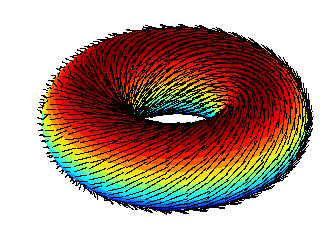
\includegraphics[width=0.2\textwidth]{figures/toroide_peloso.png}
    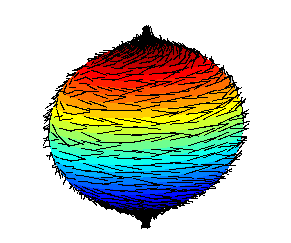
\includegraphics[width=0.2\textwidth]{figures/sfera_non_pettinabile}
    \caption{\scriptsize Un toroide pettinato ed una sfera non pettinabile (fonte: Wikipedia.)}
    \label{fig:figures-sfera_non_pettinabile}
\end{figure}
Nel caso 2-dimensionale ad esempio si ha che
\begin{redbox}{}
    La coppia di variabili azione-angolo è ben definita, infatti il toro è il prodotto di $n$ oggetti periodici.
\end{redbox}
\noindent
Tornando alle $n$ dimensioni si ha che:
\[
    I_k = \frac{1}{2\pi}\oint _{c_k} \sum_{i=1}^{n} p_idq_i
.\] 
Dove le $c_k $ sono traiettorie circuitate attorno al toro.\\
\begin{exmp}[Osillatore armonico bidimensionale.]
   \[
       H = \frac{1}{2}p_1^2+\frac{1}{2}p_2^2 + \frac{\omega_1^2}{2}q_1^2 + \frac{\omega_2^2}{2}q_2^2
   .\]  
   l'Hamiltoniana è separabile, quindi possiamo procedere definendo $\alpha_1$ e $\alpha_2$ come:
   \[
       \alpha_1 = \frac{1}{2}p_1^2+ \frac{\omega_1^2}{2}q_1^2 \qquad \alpha_2 = \frac{1}{2}p_2^2+ \frac{\omega_2^2}{2}q_2^2
   .\] 
   Abbiamo anche una coppia di azioni $I_{1,2}$:
   \[
       I_1 = \frac{1}{2\pi}\oint p_1dq_1 \qquad I_2 = \frac{1}{2\pi}\oint p_2dq_2 
   .\] 
   Mettendo tutto insieme nella Hamiltoniana trasformata finale si ottiene:
   \[
       H'(I_1,I_2) = \omega_1I_1+\omega_2I_2
   .\] 
\end{exmp}
\noindent
\subsection{Scrittura compatta del moto sul Toro}%
\label{sub:Scrittura compatta del moto sul Toro}
Il moto sul toro ha una struttura generale, possiamo riesprimerlo usando la periodicità nelle variabili azione-angolo.\\
Il nostro obiettivo finale è esprimere il moto della coordinata spaziale $q_i$ in funzione del tempo ($q_i(t)$). Nel sistema azione-angolo abbiamo che:
\[
    q_i(t) = q_i(\vect{I}, \vect{\theta}) 
.\] 
Possiamo allora cercare la decomposizione di Fourier di questa variabile nello spazio delle $I, \theta$ (essendo il moto periodico). \\
I pesi della trasformata sono:
\[
    \mathcal{A}_{\vect{k}}^{(i)}(\vect{I}) = \int_{0}^{2\pi} \theta_1 \ldots \int_{0}^{2\pi} \theta_n q_i(\vect{I}, \vect{\theta})e^{i(k_1\theta_1+ \ldots + k_n\theta_n) }   
.\] 
In cui $i$ è l'indice associato alla coordinata i-esima, $k$ è il pedice associato al $\theta$. \\
La decomposizione spettrale invece si esprime come:
\[\begin{aligned}
    q_i(t) = & \sum_{k_1=-\infty}^{\infty} \ldots\sum_{k_n = -\infty}^{\infty} \mathcal{A}_{k_1\ldots k_n}^{(i)} e^{i(k_1\theta_1+\ldots+k_n\theta_n)} =\\
	     & = \sum_{\vect{k}}^{} \mathcal{A}_{\vect{k}}^{(i)}e^{i(\vect{k}\vect{\omega} t + \vect{k}\vect{\delta}) }
.\end{aligned}\]
A questo punto la differenza tra il caso unidimensionale può esser vista in quest'ultima espressione: se gli $\omega_i$ stanno tra loro in rapporti razionali allora il moto sarà periodico chiuso, viceversa le orbite non si chiudono (nello spazio dei $q_i$).\\
In particolare per avere delle orbite chiuse servono $n-1$ relazioni del tipo:
\[
    \sum_{i=1}^{n} k_i\omega_i = 0
.\] 
\clearpage

\section{Teorema KAM}%
\label{sub:Lezione 17}
\mylocaltoc
\subsection{Sistemi quasi integrabili: teoria delle perturbazioni}%
\label{sub:Sistemi quasi integrabili: teoria delle perturbazioni}
I sistemi studiati nelle ultime due lezioni sono tutti integrabili, possiamo domandarci cosa succede nel caso di sistemi che non presentano questa caratteristica. In particolare per poter studiare tali sistemi in modo perturbativo ci concentriamo su situazioni "quasi integrabili".\\
Supponiamo di avere una Hamiltoniana del tipo:
\[
    H(I, \theta) = H_0(I) + \epsilon H_1(I, \theta  ) 
.\] 
La parte $H_0$ è integrabile, $H_1$ è la perturbazione.\\
In questo caso le equazioni di HJ sono:
\[\begin{aligned}
     & \dot{I} = - \frac{\partial }{\partial \theta  } H(I,\theta  ) \\
     & \dot{\theta} = \frac{\partial}{\partial I} H(I, \theta  ) 
.\end{aligned}\]
Vedremo che la $\dot{I}$  sarà proporzionale solo a $\epsilon$  perché la $\theta  $  compare solo nella Hamiltoniana di perturbazione.\\
All'ordine zero in $\epsilon$ si ha l'Hamiltoniana imperturbata:
\[\begin{aligned}
    & \dot{I} = - \frac{\partial H_0(I)}{\partial \theta  } = 0\\
    & \dot{\theta  }=\frac{\partial H_0(I) }{\partial I} = \omega_0(I) 
.\end{aligned}\]
Al primo ordine invece:
\[\begin{aligned}
    & \dot{I} = - \frac{\partial }{\partial \theta} H(I, \theta)= -\epsilon\frac{\partial }{\partial \theta  } H_1 + O(\epsilon^2) \\ 
    & \dot{\theta  }=\frac{\partial  }{\partial I} H(I, \theta) = \omega_0(I) + \epsilon  \frac{\partial H_1}{\partial I} 
.\end{aligned}\]
Cerchiamo una trasformazione canonica che integra al primo ordine in $\epsilon$.
\[
    \theta, I \to \varphi, J
.\] 
\[
    I = \frac{\partial }{\partial \theta  } S(\theta, J)  \qquad \varphi = \frac{\partial }{\partial J} S(\theta, J) 
.\] 
Visto che siamo al primo ordine supponiamo che la $S$  stessa sia formata dall'identità $S_0$  sommata ad un termine di perturbazione lineare in $\epsilon$.\\
Riscriviamo in questo sistema trasformato le equazioni di Hamilton Jacoby (facendo la sostituzione $I = \partial_{\theta}S$):
\begin{equation}
    H_0(\frac{\partial S}{\partial \theta} ) + \epsilon H_1(\frac{\partial S}{\partial \theta} , \theta  ) \simeq K(J) 
    \label{eq:17_H}
\end{equation}
Con $K(J)$ la nuova Hamiltoniana che, avendo fatto l'integrazione, non dipende da $\varphi$. Anche questa Hamiltoniana mi aspetto possa essere sviluppata in serie di $\epsilon$.
\[
    K(J) = K_0(J) + \epsilon  K_1(J) + \ldots
.\] 
Esplicitando l'equazione \ref{eq:17_H} all'ordine zero e uno:
\[\begin{aligned}
    & H_0(J) = K_0(J) \\
    & \frac{\partial S_1}{\partial \theta  } \frac{\partial H_0}{\partial J} + H_1(J, \theta) = K_1(J) 
.\end{aligned}\]
Il primo termine della seconda equazione deriva dal fatto che abbiamo sviluppato in serie di $\epsilon$ anche la nostra trasformazione, gli ordini successivi al primo contengono ancora la variabile $\theta$.\\
Possiamo riscrivere il primo ordine in modo da esplicitare la $K_1(J)$ introducendo anche la "frequenza" $\omega_0$:
\begin{equation}
    K_1(J) = \omega_0(J) \frac{\partial }{\partial \theta  } S_1(\theta, J) + H_1(J, \theta) 
    \label{eq:16_K1}
\end{equation}
A questo punto dobbiamo trovare due cose:
\begin{itemize}
    \item $K_1 = K_1(J) $ 
    \item $S_1$ 
\end{itemize}
Riprendendo l'equazione per $K_1(J)$ (eq \ref{eq:16_K1})  possiamo integrare in $\theta$ tra $0$ e $2\pi$, così facendo il termine $\partial_{\theta} S_1$  si annulla poiché la variabile $\theta$ è periodica (per definizione di variabili azione-angolo). \\
Di conseguenza rimane soltanto:
\[
    K_1(J) = \frac{1}{2\pi}\overline{H}_1(J,\theta) =  \frac{1}{2\pi}\int_{0}^{2\pi} H_1(J,\theta  ) d\theta 
.\] 
Questa espressione risolve il problema per $K_1(J)$ poiché nei problemi l'Hamiltoniana di perturbazione è nota. \\
Nota l'espressione di $K_1$ possiamo sostituirla nella equazione differenziale per $S_1$ (che si ottiene invertendo la \ref{eq:16_K1}):
\begin{equation}
\begin{aligned}
    \frac{\partial }{\partial \theta  } S_1(J,\theta) = & \frac{1}{\omega_0(J)}(K_1(J) - H_1(J,\theta)) = \\
							& = -\frac{1}{\omega_0(J) }(H_1(J,\theta  ) - \overline{H}_1(J,\theta) ) 
    \label{eq:17_S_1_diff}
.\end{aligned}
\end{equation}
Di conseguenza abbiamo trovato anche la $S_1$: basta integrare quest'ultima equazione in $\theta  $.\\
Fino a qui sembra tutto relativamente semplice, in maniera astratta sembra che siamo in grado di risolvere al primo ordine il sistema, tuttavia questo procedimento presenta un problema di fondo che andremo ad analizzare tra poco...\\
Proseguiamo andando in trasformata di Fourier:
\[\begin{aligned}
    & H_1 = \sum_{}^{} A_k e^{ik\theta}\\
    & S_1 = \sum_{}^{} B_k e^{ik\theta}
.\end{aligned}\]
Inseriamo nella equazione per la $\partial_{\theta} S_1$:
\[
    \partial_{\theta  }S_1(J, \theta  ) = i \sum_{}^{} kB_ke^{ik\theta} = -\frac{1}{\omega_0(J)}\sum_{k=1}^{} A_ke^{ik\theta  }
.\] 
L'ultima sommatoria parte da $1$  poiché abbiamo rimosso il valor medio che era presente nella equazione a sottrarre.\\
La struttura della $S_1$  è definita dai $B_k$, questi possiamo esplicitarli in funzione degli $A_k$:
\begin{equation}
    B_k = \frac{iA_k}{k\omega_0(J)}
    \label{eq:17_esp_S_1}
\end{equation}
Quindi in conclusione:
\[
    S_1(J, \theta) = \sum_{k}^{} \frac{iA_ke^{ik\theta  }}{k\omega_0(J) }
.\] 
A questo punto noi sappiamo che la $S$ al primo ordine si scrive come:
\[
    S = J\theta +\epsilon S_1
.\] 
Quindi siamo in grado di trovare tutte le quantità utili allo studio del moto:
\[\begin{aligned}
    & \phi  = \theta +\epsilon\partial_{J}S_1(J,\theta  ) \\
    & J = I - \epsilon\partial_{\theta  }S_1(J,\theta) \\
    & \omega (J) = \omega_0(J) + \epsilon\partial_{J}K_1(J) 
.\end{aligned}\]
In una dimensione è quindi tutto integrabile e risolubile. 
\begin{exmp}[Oscillatore armonico perturbato]
    \[
	H(p,q) = \frac{1}{2}p^2+\frac{1}{2}\omega_0^2q^2 + \epsilon H_1 
    .\] 
    \textbf{Caso }$H_1 = q^4$.\\
    Possiamo partire dalla soluzione alla Hamiltoniana imperturbata (è stata risolta esplicitamente, vedi come si deriva la \ref{eq:16_q}):
    \[
	H_0=\omega_0I \qquad q = \sqrt{\frac{2I}{\omega_0}} \sin (\theta  ) \qquad
        \theta =\omega_0t
    .\] 
    Quindi inserendo nel termine di perturbazione la $q$ si ha:
    \[
	H_1(I,\theta  ) = \left(\frac{2I}{\omega_0}\right)^{2}\sin^4(\theta) 
    .\] 
    A questo punto possiamo procedere con due metodi:
    \begin{itemize}
	\item Calcolare la trasformata di $H_1$, i coefficienti di tale espansione in serie di Fourier saranno legati a quelli della $S_1$ dalla relazione \ref{eq:17_esp_S_1}.
	\item Trovare la $K_1$, esprimere la $S_1$ tramite l'equazione differenziale \ref{eq:17_S_1_diff}.
    \end{itemize}
    In entrambi i casi si raggiunge il medesimo risultato, proviamo ad applicare il secondo metodo "più esplicito".\\
    Procediamo con l'espansione della $H$ al primo ordine effettuando la trasformazione:
    \[
	H_0(\partial_{\theta}S)+\epsilon H_1(\partial_{\theta}S,\theta) = K(J)
    .\] 
    La trasformazione può anch'essa essere sviluppata, esplicitiamo anche la derivata (ricordando che il termine perturbato dipende da $\theta$):
    \[
        S = \theta J + \epsilon S_1 \implies  \partial_{\theta}S = J + \epsilon\partial_{\theta}S_1
    .\] 
    Reinseriamo il tutto nella $H$ al primo ordine:
    \[
	\omega_0\partial_{\theta}S + \epsilon\left(\frac{2\partial_{\theta}S}{\omega_0}\right)^2\sin^4\theta =K(J)
    .\] 
    \[
	\omega_0(J + \epsilon\partial_{\theta}S_1)+ \epsilon\left(\frac{2J}{\omega_0}\right)^2\sin^4\theta =K(J)
    .\] 
    Visto che ci interessa soltanto il primo ordine in $\epsilon$ si butta il termine dipendente da $\epsilon$ nella parentesi del secondo termine.\\
    Possiamo riscrivere quest'ultima equazione in termini della $H_1$:
    \[
	\omega_0\partial_{\theta}S_1(\theta,J) = K_1(J)-H_1(J,\theta)
    .\]
    Quindi si trova la $K_1$ come valor medio di $H_1$ su un periodo:
    \[\begin{aligned}
	K_1&(J)= \frac{1}{2\pi} \int_{0}^{2\pi} H_1(\theta,J)d\theta =\\
	       & = \frac{1}{2\pi}\int_{0}^{2\pi} \left(\frac{2J}{\omega_0}\right)^2 \sin^4(\theta)d\theta =\\
	       & = \frac{1}{2\pi}\left(\frac{2J}{\omega_0^2}\right)\left[\frac{3}{8}\theta-\frac{1}{2}\sin(2\theta)  + \frac{1}{32}\sin (4\theta)\right]_{0}^{2\pi}=\\
	       & = \frac{3}{8}\left(\frac{2J}{\omega_0}\right)^2
    .\end{aligned}\]
    Quindi inseriamo nella equazione differenziale per $S_1$:
    \[
	\omega_0\partial_{\theta}S_1(\theta,J) = \left(\frac{2J}{\omega_0}\right)^2 \left[\frac{3}{8}-\sin^4\theta\right]
    .\] 
    Effettuiamo un integrale indefinito:
    \[\begin{aligned}
	S_1&(\theta,J)=\\
	&=\frac{4J^2}{\omega_0^3}\left[\frac{3}{8}\theta-\left(\frac{3}{8}\theta-\frac{1}{2}\sin(2\theta) +\frac{1}{32}\sin(4\theta)\right)\right]=\\
		      &= \frac{4J^2}{\omega_0^3} \left(\frac{1}{2}\sin(2\theta) -\frac{1}{32}\sin(4\theta)\right)
    .\end{aligned}\]
    Notiamo che le due funzioni rimaste in $S_1$ sono entrambe periodiche in $\theta$.\\
    A questo punto abbiamo tutto, la nuova Hamiltoniana ad esempio:
    \[
	K(J) = K_0 + \epsilon K_1 = \omega_0J + \epsilon \frac{3}{8}\left(\frac{2J}{\omega_0}\right)^2
    .\] 
    Il vecchio momento:
    \[
	I = \frac{\partial }{\partial \theta}(S_0 + \epsilon S_1)=J+\frac{\epsilon}{\omega_0}\left(\frac{2J}{\omega_0}\right)^2\left[\frac{3}{8}-\sin^4\theta\right]
    .\] 
    la frequenza:
    \[
	\omega (J)=\frac{\partial }{\partial J} K(J) = \omega_0 + \epsilon  \frac{3J}{\omega_0^2}
    .\] 
    La nuova variabile angolo:
    \[\begin{aligned}
	\phi =& \frac{\partial }{\partial J} (S_0+ \epsilon S_1) = \\
	      & = \theta + \epsilon \frac{8J^2}{\omega_0^3}\left(\frac{1}{2}\sin(2\theta) - \frac{1}{32}\sin(4\theta)\right)
    .\end{aligned}\]
    Notiamo che la perturbazione in questo caso "irrigidisca" il potenziale che era in precedenza armonico, infatti la frequenza di oscillazione al primo ordine che abbiamo ottenuto aumenta all'aumentare dell'energia ($J$) linearmente.\\
    \textbf{Caso $H_1 = q^3$}.\\
    In questo caso, effettuando i medesimi passaggi, ci si rende conto che la correzione al primo ordine in $\epsilon$ si annulla ($K_1 \propto\overline{H}_1 = 0$ ). \\
    Dobbiamo quindi espandere perturbativamente al secondo ordine, i risultati che si ottengono sono:
    \[
	K_2(J)= -\frac{15\pi J^2}{2\omega_0^4}
    .\] 
    \[
	\omega (J)=\omega_0-\epsilon^2 \frac{15\pi J}{\omega_0^4}
    .\] 
\end{exmp}
\noindent
In una dimensione il problema è sempre risolubile perturbativamente. Sarà così anche in dimensioni maggiori?
\subsection{Sviluppo perturbativo in due dimensioni}%
\label{sub:Sviluppo perturbativo in due dimensioni}
Prendiamo i due vettori per le variabili azione-angolo:
\[
    \vect{I} = (I_1,I_2) \qquad \vect{\theta} = (\theta_1, \theta_2)
.\] 
l'Hamiltoniana al primo ordine perturbativo è sempre:
\[
    H(\vect{I}, \vect{\theta}) = H_0(\vect{I}) + \epsilon V(\vect{I}, \vect{\theta})
.\] 
Con $V$ termine di perturbazione. Possiamo decomporre la perturbazione nella base dei $\vect{\theta}$ facendo una trasformata di Fourier:
\[
    H(\vect{I}, \vect{\theta}) = H_0(\vect{I}) + \epsilon \sum_{n_1}^{} \sum_{n_2}^{} V_{n_1,n_2}\cos (n_1\theta_1+n_2\theta_2)
.\] 
Con $n_1,n_2 \in \mathbb{Z}$. Scriviamo in notazione vettoriale anche $ (n_1,n_2)$:
\[
    \vect{n} =(n_1,n_2) \qquad n_1\theta_1+n_2\theta_2 = \vect{n}\cdot \vect{\theta}
.\] 
Chiamiamo questa volta la trasformazione $G$ anziché $S$:
\[
    G(\vect{J}, \vect{\theta})=\vect{J}\cdot \vect{\theta} + \epsilon\sum_{ n_1}^{} \sum_{n_2}^{} g_{n_1,n_2}(\vect{J})\sin (\vect{n}\cdot \vect{\theta})
.\] 
Con $g_{n_1,n_2}$ coefficienti non (ancora) fissati per la trasformazione.\\
Possiamo esprimere anche la componente $i$-esima di $I$:
\[
    I_i = \frac{\partial G}{\partial \theta_i} =
    J_i + \epsilon\sum_{ n_1}^{} \sum_{n_2}^{} n_ig_{n_1,n_2}(\vect{J})\cos (\vect{n}\cdot \vect{\theta})
.\] 
Allo stesso modo per il nuovo angolo $\vect{\varphi}$:
\[
    \varphi_i = \frac{\partial G}{\partial J_i} =
    \theta_i + \epsilon  \sum_{n_1}^{} \sum_{n_2}^{} \frac{\partial }{\partial J_i} (g_{n_1,n_2}(\vect{J}))\sin (\vect{n}\cdot \vect{\theta})
.\] 
A questo punto si scrive la nuova Hamiltoniana $H'(\vect{J}, \vect{\varphi})$, per farlo sfruttiamo la scrittura del primo ordine perturbativo data dalla \ref{eq:16_K1} generalizzata in due dimensioni:
\[
    K_1(\vect{J})=\frac{\partial S_1}{\partial \vect{\theta}} \cdot \vect{\omega} + H_1(\vect{J,\vect{\theta}})
.\] 
Con la frequenza data da:
\[
    \vect{\omega} = \frac{\partial H_0(\vect{J})}{\partial \vect{J}} 
.\] 
Notiamo che si tratta proprio della Hamiltoniana $H_0$, per trovare queste frequenze operativamente (all'ordine 0) basta sostituire il simbolo $\vect{J}$ a quello $\vect{I}$ e derivare, deriva dalla definizione della trasformazione canonica che vogliamo fare!\\
Quindi in conclusione:
\[\begin{aligned}
    H'(\vect{J},\vect{\varphi}) = & 
    H_0(\vect{J}) + \epsilon  \sum_{}^{} \vect{n}\cdot \vect{\omega} g_{\vect{n}}(\vect{J})\cos (\vect{n}\cdot \vect{\theta}) +\\
				  & + \epsilon  \sum_{}^{} V_{\vect{n}}(\vect{J})\cos (\vect{n}\cdot \vect{\theta}) + O(\epsilon^2)
.\end{aligned}\]
Salta all'occhio che possiamo far sparire il termine in $\epsilon$  scegliendo un set opportuno di $g_{\vect{n}}$:
\[
    g_{\vect{n}}= - \frac{V_{\vect{n}}(\vect{J})}{n_1\omega_1+n_2\omega_2}
.\] 
Se si scelgono questi $g$ si rende l'Hamiltoniana di partenza integrabile.
\[
    H'(\vect{J}, \vect{\varphi}) = H_0(\vect{J})
.\] 
Inoltre, per completezza, esplicitiamo anche la forma della vecchia variabile $\vect{I}$:
\[
    \vect{I}  = \vect{J}-\epsilon\sum_{}^{} \frac{\vect{n} V_{\vect{n}}\cos (\vect{n}\cdot \vect{\theta})}{\vect{n}\cdot \vect{\omega}}
.\] 
Notiamo che sorge subito un problema: se il prodotto scalare $\vect{n}\cdot \vect{\omega}$ si annulla la teoria perturbativa si rompe.\\
Il fatto è che $g_{\vect{n}}$ è il coefficiente di uno sviluppo di Fourier bidimensionale, nel quale si somma sui numeri $n_1,n_2 \in \mathbb{Z}$.\\
In generale quindi succederà che un termine della sommatoria romperà lo sviluppo se le due frequenze $\omega_1$ e $\omega_2$ sono numeri razionali.\\
\subsection{Esempio di rottura della teoria perturbativa}%
\label{sub:Esempio di rottura della teoria perturbativa}
Prendiamo ad esempio una Hamiltoniana bidimensionale del tipo:
\[
    H = H_0(\vect{I})+\epsilon V_{\vect{n}}(\vect{I})\cos (n_1\theta_1-n_2\theta_2)=E
.\] 
Con $E$ costante. Per una $H$ di questo tipo abbiamo che esiste un integrale del moto $c_2$ tale che:
\[
    c_2=n_1I_2+n_2I_1
.\] 
Questo perché, dalle equazioni di Hamilton:
\[\begin{aligned}
    & \partial_{t}I_1 = -\partial_{\theta_1}H = \epsilon n_1 V_{\vect{n}}\sin (\vect{n}\cdot \vect{\theta})\\
    & \partial_{t}I_2 = -\partial_{\theta_2}H = - \epsilon n_2 V_{\vect{n}}\sin (\vect{n}\cdot \vect{\theta})
.\end{aligned}\]
Quindi si ha banalmente che:
\[
    \dot{c}_2 = \partial_{t}(n_1I_2+n_2I_1) = 0
.\] 
Sfruttiamo questo integrale per studiare il caso con un esempio concreto.
\paragraph{Caso particolare}%
\label{par:Caso particolare_17}
\begin{equation}
    H = H_0(\vect{I})+ \alpha I_1I_2\cos (2\theta_1-2\theta_2) = E
    \label{eq:Caso particolare_17}
\end{equation}
Con $E$ costante. In questo caso abbiamo $n_1 = -n_2 = 2$ per essere espliciti.
L'Hamiltoniana imperturbata è definita da:
\[
    H_0(\vect{I}) = I_1 + I_2 - I_1^2 - 3I_1I_2 + I_2^2
.\] 
Per risolvere conviene prima fare un cambio di variabili: 
\[
    J_1=I_1+I_2 \qquad J_2 = I_2
.\] 
\[
    \varphi_1 = \theta_2 \qquad \varphi_2 = \theta_2-\theta_1
.\] 
Le equazioni di Hamilton del sistema sono:
\[\begin{aligned}
    & \dot{J}_1 = 0\\
    & \dot{J}_2 = 2\alpha J_2(J_1-J_2)\sin (2\varphi_2)\\
    & \dot{\varphi}_1 = 1-2J_1-J_2+\alpha J_2\cos (2\varphi_2)\\
    & \dot{\varphi }_2=-J_1+6J_2+\alpha (J_1-2J_2)\cos (2\varphi_2)
.\end{aligned}\]
Quindi partendo dalla prima equazione possiamo ricavare gli andamenti temporali di tutte le quantità: $J_1(t),\varphi_2(t), J_2(t), \varphi_1(t)$.\\
Applichiamo adesso il meccanismo perturbativo per integrare l'Hamiltoniana. Sappiamo che la trasformazione dovrebbe essere della forma:
\[
    G(\vect{L}, \vect{\varphi}) = \vect{L}\cdot \vect{\varphi}  + \alpha g_{22}(\vect{ L})\sin (2\varphi_1-2\varphi_2)
.\] 
Il coefficiente dell sviluppo $g$ (anche detto termine di perturbazione):
\[
    g_{_{22}} = - \frac{L_1L_2}{2\omega_1-2\omega_2}
.\] 
Le vecchie variabili $\vect{J}$ possono essere ottenute dalle nuove come:
\[\begin{aligned}
    & J_1(\vect{\theta}) = L_1 - \frac{2\alpha L_1L_2 \cos (2\omega_1 t-2\omega_2 t)}{2\omega_1-2\omega_2}\\
    & J_2(\vect{\theta}) = L_2 - \frac{2\alpha L_1L_2 \cos (2\omega_1 t-2\omega_2 t)}{2\omega_1-2\omega_2}
.\end{aligned}\]
Possiamo ottenere le frequenze nelle nuove variabili (all'ordine più basso) effettuando la derivata della Hamiltoniana imperturbata:
\[
    \vect{\omega} (\vect{L})= \frac{\partial H_0(\vect{L})}{\partial \vect{L}} 
.\] 
Dove $H_0(\vect{L})$ è l'Hamiltoniana di partenza (sostituendo $\vect{I}\to \vect{L}$).
In componenti si ottiene:
\[\begin{aligned}
    & \omega_1( L_1,L_2) = 1-2L_1-3L_2\\
    & \omega_2(L_1,L_2) = 1-3L_1+2L_2
.\end{aligned}\]
Non è ovvio quindi che, al variare di $L_1,L_2$, il denominatore del termine di perturbazione resti sempre molto maggiore di zero.\\
Se tale termine dovesse diventare molto più piccolo del numeratore la teoria perturbativa si rompe. \\
La condizione per il quale vale la teoria perturbativa è:
\[
    \left|2\omega_1-2\omega_2\right| = \left|2L_1-10L_2\right|\gg 2\alpha L_1L_2
.\] 
Con $\alpha$ coefficiente sul quale si sviluppa la teoria perturbativa. La domanda adesso è: visto che non possiamo sapere a priori come sono fatte le $\omega$ come facciamo a capire quando si applica la teoria perturbativa?
\subsection{Teorema KAM}%
\label{sub:Teorema KAM}
Il teorema KAM ci dice quando è possibile costruire una teoria perturbativa per un sistema Hamiltoniano.\\
Data una Hamiltoniana del tipo:
\[
    H(I,\theta)= H_0(I)+H_1(I,\theta)
.\] 
Con $H_1$ "piccola" e 
\[
    H_1(J,\theta +2\pi) = H_1(J,\theta)
.\] 
Consideriamo un Toro $T_0$ nello spazio delle fasi (per il problema senza perturbazione) caratterizzato da un set di frequenze $\vect{\omega}^*$ irrazionali:
\[
    \vect{k}\cdot \vect{\omega}^* \neq 0 \quad \forall \vect{k}
.\] 
Sappiamo che valgono le seguenti espressioni che caratterizzano il flusso sul toro $T_0$:
\[\begin{aligned}
    & I = I^* = \text{costante}\\
    & \dot{\theta} = \omega^*
.\end{aligned}\]
Inoltre, sempre per ipotesi, assumiamo che l'Hessiano della trasformazione sia non nullo:
\[
    \frac{\partial ^2 H_0}{\partial J_i \partial J_j} \neq 0
.\] 
Se l'Hamiltoniana di perturbazione $H_1$ è sufficientemente piccola allora esiste un toro invariante $T(\omega^*)$ del sistema perturbato vicino al toro non perturbato $T_0(\omega^*)$, il Toro $T(\omega^*)$ è una piccola deformazione del toro precedente.\\
Quindi, come già accennato, questo vale per frequenze di risonanza tra loro irrazionali.\\
Nella dimostrazione del teorema si scopre che i tori, al variare delle costanti del moto, si spaccano uno dietro l'altro. I primi a rompersi sono proprio quelli con $\omega$ "più" razionali tra loro. \\
Nella seguente sezione analizziamo cosa significa essere più meno razionali per un numero.
\subsubsection{Frazioni continue e most irrational number}%
\label{subsub:Frazioni continue e most irrational number}
Un qualunque numero irrazionale può essere espresso come frazione continua:
\[
    \omega  = \left[a_0,a_1,\ldots\right] = a_0 + \frac{1}{a_1+\frac{1}{a_2+\frac{1}{\ldots}}}
.\] 
Un numero razionale $\overline{\omega}$ è un numero che tronca la serie ad un termine finito, troncare la serie al termine $j$-esimo implica che $a_j = \infty$:
\[
    \overline{\omega} = \left[a_1, \ldots, a_{j-1}, \infty\right]
.\] 
Possiamo chiederci quale sia il numero più irrazionale possibile, ovvero un numero composto da una infinita serie di $a_i$ tale che:
\[
    x = \frac{1}{1+\frac{1}{1+ \ldots}}
.\] 
I coefficienti sono tutti unitari, infatti se un termine $a_i$ ad un certo punto fosse maggiore degli altri allora sarebbe possibile troncare la serie approssimandola (come se fosse un $\infty$).\\
Il numero $x$ presenta un comportamento di self similarità, quindi possiamo troncare il suo denominatore reintroducendo se stesso:
\[
    x \simeq \frac{1}{1+x} \implies  x^2+x-1=0
.\] 
La soluzione di questa equazione di secondo grado è il rapporto aureo:
\[
    x = \frac{-1 \pm \sqrt{5}}{2}
.\] 
Quindi il toro più duro, ovvero quello che si rompe per ultimo, è quello avente rapporto tra le frequenze dato dal rapporto aureo.
\clearpage

\section{Lezione 18}%
\label{sub:Lezione 18}
\subsection{Visualizzare la dinamica: mappa di Poincare}%
\label{sub:Visualizzare la dinamica: mappa di Poincare}
Siamo interessati a capire come visualizzare il caos quando andiamo in dimensioni superiori a $1$, questo perché vorremmo studiare almeno il caso 2D, però non siamo in grado di plottare uno spazio delle fasi a quattro dimensioni. \\
Un metodo molto popolare è quello di sfruttare le \textbf{mappe di Poincare}.\\
Prendiamo una Hamiltoniana del seguente tipo:
\[
    H = \frac{p_x^2}{2}+\frac{p_y^2}{2} + V(x, y)
.\] 
L'idea di fondo delle mappe di Poincare è quello di catturare il moto in 4 dimensioni su una sezione, la sezione che si sceglie è:
\[\begin{aligned}
    & p_y>0\\
    & y=0
.\end{aligned}\]
\begin{figure}[H]
    \centering
    \incfig{18_flux_line}
    \caption{\scriptsize Le traiettorie nello spazio delle fasi a quattro dimensioni, essendo su dei tori, possono essere immaginate come delle curve che girano su loro stesse. La proiezione che cerchiamo sono i punti che intersecano il piano rosso ($y=0$) ed allo stesso tempo entrano nel foglio (vogliamo $p_y>0$). In questo modo si ottiene una traiettoria descritta dai punti verdi scuri, uniti dalla linea verde chiara. Le croci rosse sono i punti che arrivano in $y=0$ ma vanno esclusi poiché hanno $p_y<0$ (il segno di $p_y$ è espresso dalla direzione della freccia quando entra nel piano $y=0$).}
    \label{fig:18_flux_line}
\end{figure}
\noindent
Non è facile da spiegare, è più facile da vedere: ti lascio il link all'indiano che te lo spiega (clicca \href{https://www.youtube.com/watch?v=PR5Ds5iS3Ow}{QUI}).\\
Vediamo un esempio pratico riprendendo un sistema già analizzato nella lezione precedente (\ref{eq:Caso particolare_17}).
\subsection{Mappa di Poincare per sistema con una costante del moto}%
\label{sub:Mappa di Poincare per sistema con una costante del moto}
   \[
    H = H_0(\vect{I})+ \alpha I_1I_2\cos (2\theta_1-2\theta_2) = E
.\] 
Con $E$ costante e: 
\[
    H_0(\vect{I}) = I_1 + I_2 - I_1^2 - 3I_1I_2 + I_2^2
.\] 
Il cambio di variabili effettuato per applicare il metodo perturbativo è:
\[
    J_1=I_1+I_2; \quad J_2=I_2; \quad \varphi_1 = \theta_2; \quad \varphi_2=\theta_2-\theta_1
.\] 
In questo modo appare la costante del moto $J_1$, le equazioni di HJ sono:
\[\begin{aligned}
    & \dot{J}_1 = 0\\
    & \dot{J}_2 = 2\alpha J_2(J_1-J_2)\sin (2\varphi_2)\\
    & \dot{\varphi}_1 = 1-2J_1-J_2+\alpha J_2\cos (2\varphi_2)\\
    & \dot{\varphi }_2=-J_1+6J_2+\alpha (J_1-2J_2)\cos (2\varphi_2)
.\end{aligned}\]
E quindi l'Hamiltoniana:
\[
    H(\vect{J},\vect{\varphi}) = J_1 - J_1^2 - J_1J_2 + 3J_2^2 + \alpha  J_2(J_1-J_2)\cos (2\varphi_2)
.\] 
Ormai siamo abituati a scrivere l'Hamiltoniana in termine delle variabili azione-angolo $I,\theta$ (oppure $J,\varphi$), per visualizzare la dinamica dobbiamo tornare indietro nelle variabili $p, q$. \\
Per farlo dobbiamo applicare passaggi analoghi a quelli di \ref{eq:16_q}, in tal caso si è esplicitato come trovare $q$, per trovare $p$ basta fare $\partial_{q}S(q,J)$. In questo caso si assume inoltre $\omega_0=1$.
\begin{equation}
\begin{aligned}
    & p_i = - \sqrt{2J_i} \sin\varphi_i\\
    & q_i = \sqrt{2J_i} \cos\varphi_i
    \label{eq:18_H_22}
.\end{aligned}\end{equation}
Si può esprimere le variabili $J_i, \varphi_i$ in funzione delle $q_i$ e delle $p_i$ per poi reinserirle nella Hamiltoniana.
\[
    J_1 = \frac{p_1^2+q_1^2}{2} \qquad J_2 = \frac{p_2^2+q_2^2}{2}
.\] 
\[\begin{aligned}
    \cos (2\varphi_2) =& \cos^2\varphi-\sin^2\varphi  =\\
    =& -\left(\frac{p_2^2-q_2^2}{2J_2}\right) = -\left(\frac{p_2^2-q_2^2}{2(p_2^2+q_2^2)}\right)
.\end{aligned}\]
Giusto per referenza l'Hamiltoniana in termini di $\vect{p}, \vect{q}$ sarebbe:
\[\begin{aligned}
    H(\vect{p}, \vect{q})=& \frac{p_1^2+q_1^2}{2}-\left(\frac{p_1^2+q_1^2}{2}\right)^2 + \\
			  & - \left(\frac{p_1^2+q_1^2}{2}\right)\left(\frac{p_2^2+q_2^2}{2}\right) +3\left(\frac{p_2^2+q_2^2}{2}\right)^2 + \\
			  & - \frac{(p_2^2-q_2^2)}{4}\left(p_1^2-p_2^2 + q_1^2-q_2^2\right)
.\end{aligned}\]
\paragraph{Ottenere la mappa}%
\label{par:Ottenere la mappa}
In questo caso particolare conviene risolvere il problema nelle variabili $J_i, \phi_i$, successivamente applicare le trasformazioni \ref{eq:18_H_22} per tornare nello spazio $p,q$.\\
Possiamo notare che, fissando l'energia $E$ del sistema ed avendo un'integrale del moto ($J_1$), il problema è completamente risolto: non c'è bisogno di fissare alcun piano (tipo $y=0$) come detto nel caso generale della sezione precedente.\\
Infatti senza alcun integrale del moto si hanno 4 gradi di libertà, la presenza di $E$ e $J_1$ ne lascia soltanto 2 a disposizione. Nel seguito si sceglie di lasciare liberi soltanto $J_{2}$ e $\phi_2$ (quindi si plotta $p_y$ in funzione di $y$).\\
Si elencano operativamente i passaggi da seguire per ottenere la mappa:
\begin{enumerate}
    \item Selezionare energia e $\alpha$ iniziali. 
    \item Selezionare un parametro $J_1$ iniziale e farlo variare in un intervallo ragionevole (vedere Linda Reichl, pag. 28-31).
    \item Sulla base della scelta di $J_1$ fissare $J_2$ e $\phi_2$ in modo da conservare l'energia. Per far questo è necessario invertire l'Hamiltoniana per trovare $J_2$:
	\[\begin{aligned}
	    &\left[3-\alpha\cos (2\phi_2)\right]J_2^2 + \\
	    & \quad \left[\left(\alpha\cos (2\phi_2)-1\right)J_1\right]J_2 + \left[J_1-J_1^2 - E\right] = 0
	.\end{aligned}\]
	Per trovare un intervallo dove le soluzioni esistono è necessario che il discriminante $\Delta$ di questa equazione sia positivo, imponendo $\Delta > 0$ si fissa quindi un possibile $\phi_2$.
    \item Integrare le equazioni \ref{eq:18_H_22} con un metodo appropriato, io ho scelto integratore di Heun (senza parte stocastica) come il professore.
    \item Tornare nelle variabili $y, p_y$ con la trasformazione canonica.
    \item Plottare $p_y$ vs $y$.
\end{enumerate}
Vi assicuro che i punti (2) e (3) non sono affatto divertenti: il dominio di esistenza di questi parametri non è molto vasto, fatevi guidare dal libro sopra citato, dallo script di Fortran del professore (mapH22.f) e dal notebook caricato su Github.\\
Se sarete pazienti otterrete la seguente mappa:
\begin{figure}[H]
    \centering
    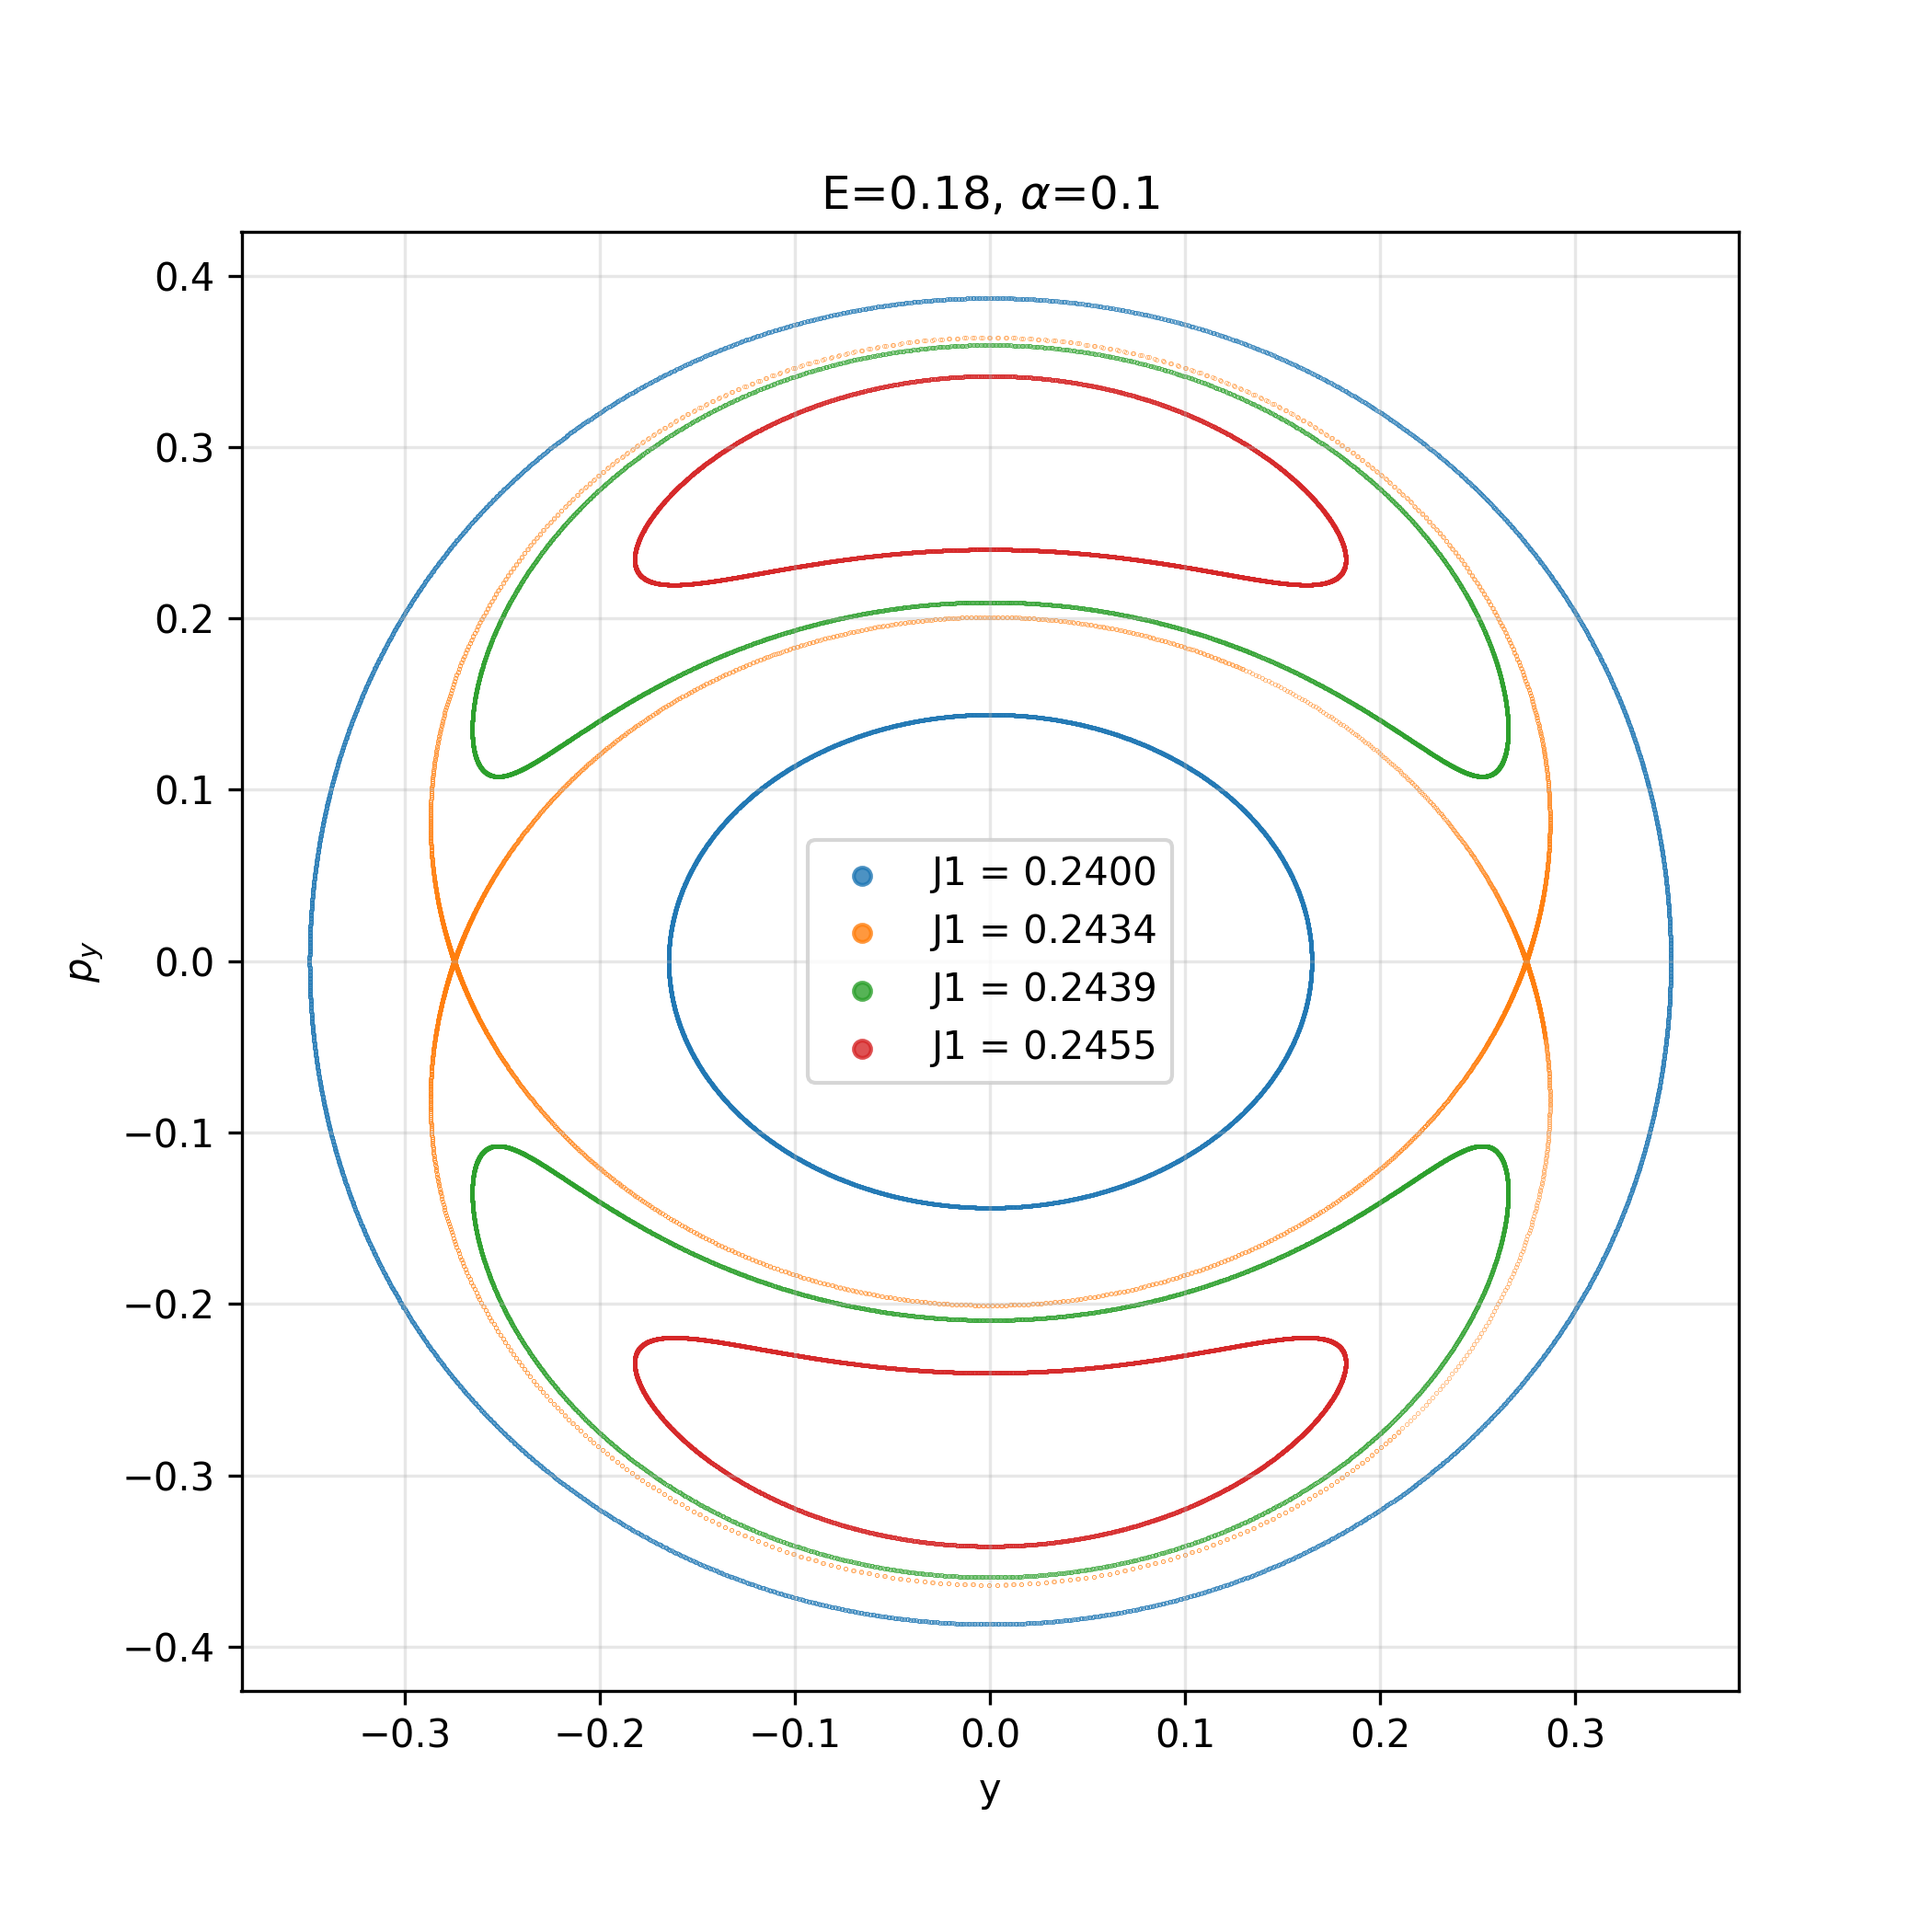
\includegraphics[width=0.5\textwidth]{figures/18_H22.png}
    \caption{\scriptsize Mappa di Poincare per il sistema bidimensionale di questa sezione, notiamo la risonanza in $J_1 = 0.24$. Per $\alpha\ll 1$ si dovrebbe avere la risonanza a $I_1\simeq 5I_2$. Numericamente questa non è esattamente rispettata, probabilmente $\alpha=0.1$ non basta.}
    \label{fig:figures-18_H22-png}
\end{figure}
\subsection{Sistema di Henon e Heiles: sono stabili le stelle delle galassie?}%
\label{sub:Sistema di Henon e Heiles}
Nel 1964 era noto che, il moto di una stella nella galassia presentava due integrali del moto: l'energia ed una componente del momento angolare.\\
Analiticamente nessuno riusciva a capire se fosse presente un altro integrale del moto, tuttavia le osservazioni del rapporto tra la velocità parallela al centro della galassia e quella ortogonale ne suggerivano la presenza (tale rapporto risultava circa 2:1).\\
Henon e Heiles ci riuscirono nell'intento modellizzando con una semplice Hamiltoniana:
\[
    H = \frac{1}{2}(p_x^2+p_y^2) + \frac{1}{2}(x^2+y^2) + x^2y-\frac{1}{3}y^3
.\] 
Quello che fecero è studiare la mappa: se si fosse presentata una terza costante del moto sarebbe apparsa nel numero di tori invarianti del sistema.
\begin{figure}[H]
    \centering
    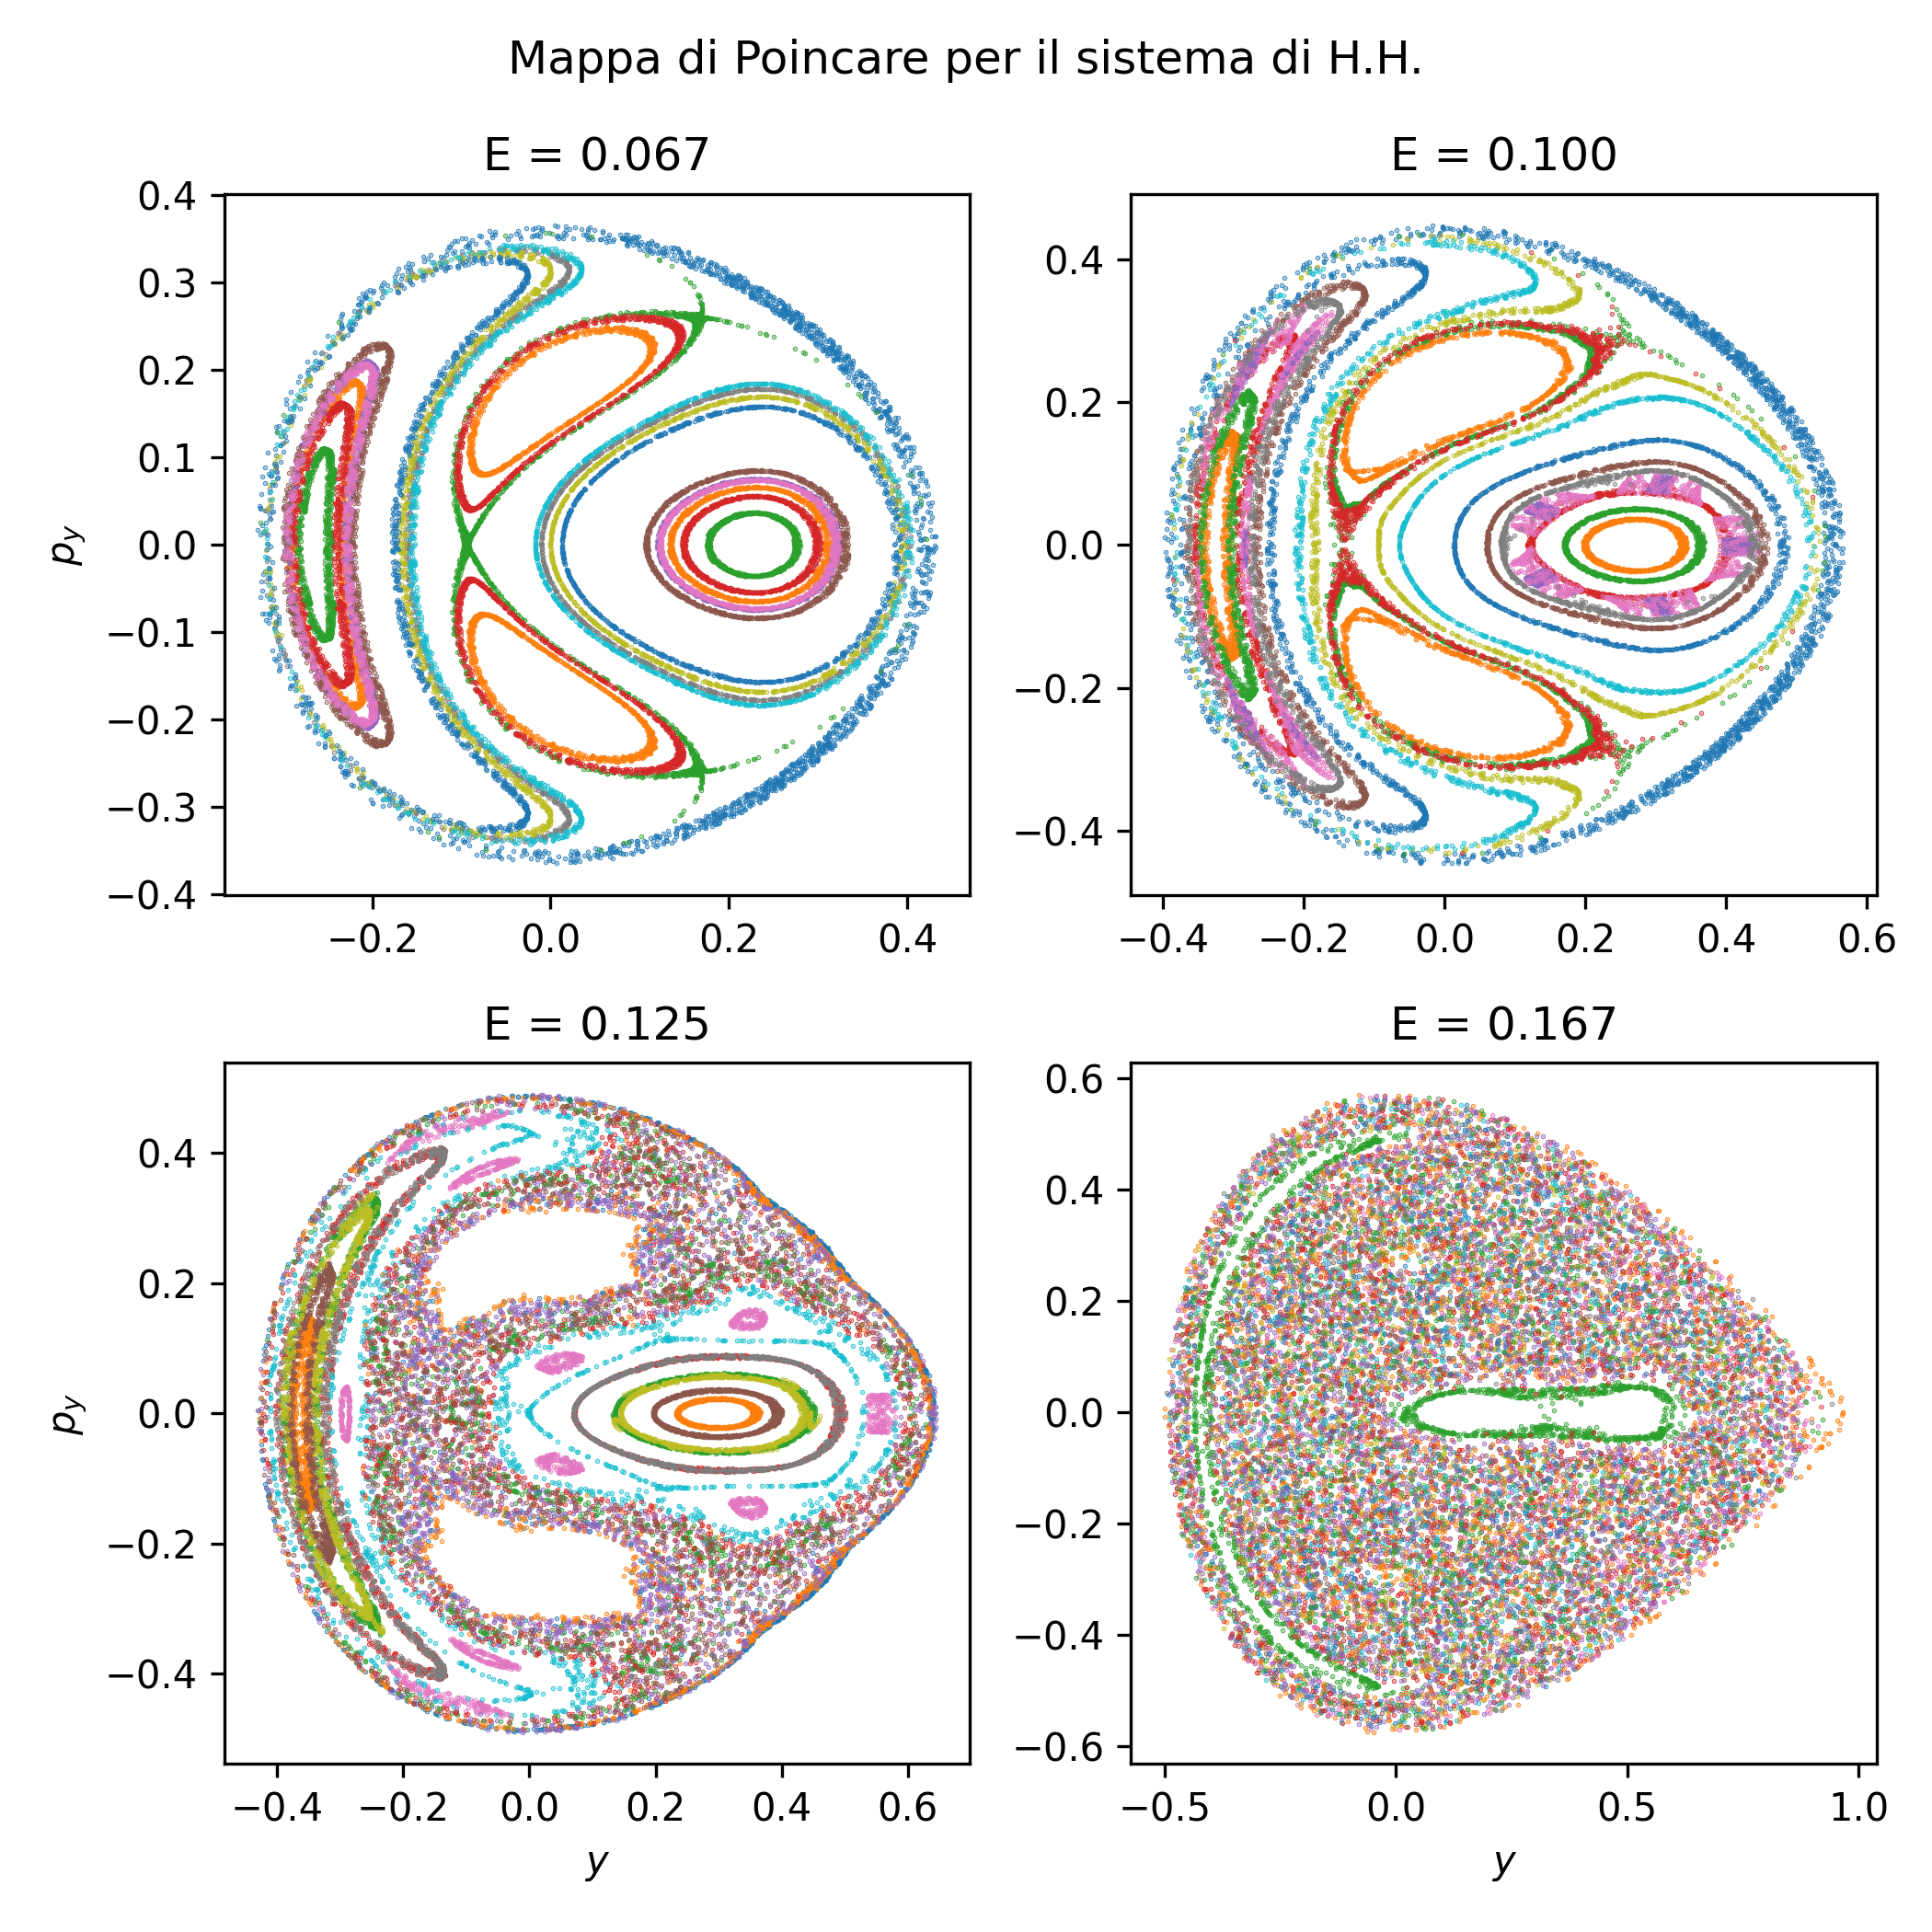
\includegraphics[width=0.45\textwidth]{figures/18_Henon-Heiles.png}
    \caption{\scriptsize Mappa di Poincare per il sistema di Henon-Heiles: notiamo come a bassa energia è evidente la presenza di tori invarianti: c'è un terzo integrale del moto.}
    \label{fig:}
\end{figure}
\noindent
Si vede bene che, all'aumentare della energia, i tori invarianti si rompono. In particolare si ha che i primi tori a rompersi sono proprio quelli passanti per il punto fisso: quelli corrispondenti a delle frequenze di H tra loro razionali.
\subsubsection{Tentativo di costruire una teoria perturbativa per Henon-Heiles}%
\label{subsub:Tentativo di costruire una teoria perturbativa per Henon-Heiles}
Il motivo per il quale non è stato possibile trovare un terzo integrale del moto analiticamente è il fallimento della teoria perturbativa. Andiamo in variabili azione-angolo:
\[
    \frac{1}{2}p_x^2 + \frac{1}{2}x^2 = \omega_xI_x
.\] 
\[
    \frac{1}{2}p_y^2 + \frac{1}{2}y^2 = \omega_yI_y
.\] 
Le trasformazioni canoniche associate sono:
\[\begin{aligned}
    x = \sqrt{2I_x} \sin\theta_x \qquad y = \sqrt{2I_y} \sin\theta_y
.\end{aligned}\]
In conclusione possiamo scrivere l'Hamiltoniana imperturbata come:
\[
    H_0 = \omega_xI_x + \omega_yI_y
.\] 
Mentre la perturbazione:
\[\begin{aligned}
    H_I = &\frac{(2I_x)(2I_y)^{1 /2}}{2}\times\\ 
	  &\times \left[\sin \theta_y-\frac{1}{2}\sin (\theta_x+\theta_y)-\frac{1}{2}\sin (\theta_x-2\theta_x) \right] + \\
	  & - \frac{1}{3}\left(2I_y\right)^{3 /2}\left[\frac{3}{2}\sin\theta_y-\frac{1}{2}\sin (3\theta_y)\right]
.\end{aligned}\]
In conclusione si dovrebbe trovare la trasformazione che integra la seguente H:
\[
    H = H_0+H_I
.\] 
Il grosso problema è che possiamo trovarne una che elimini una delle due risonanze in $\theta_y\pm 2\theta_x$
\footnote{Il problema di questi termini deriva dalla \textbf{interazione} delle due variabili angolo: tale interazione potrebbe distruggere la teoria perturbativa per la scelta di determinati valori iniziali ad esempio.}
, non è tuttavia possibile eliminarle entrambe. La teoria perturbativa quindi fallisce in questo caso e vediamo i tori nello spazio delle fasi rompersi all'aumentare dell'energia.\\
Nel seguito ci focalizzeremo su delle mappe che siano "\textbf{Area preserving}", ovvero quelle che derivano da sistemi Hamiltoniani.\\
Una mappa, per essere area preserving deve avere uno Jacobiano unitario, in due dimensioni ad esempio dovrà essere:
\[
    \frac{\partial (x_{i+1}, y_{i+1})}{\partial (x_i, y_i)} = 1
.\] 
La logica di questo cambio di punto di vista è la seguente: se studiamo degli insiemi generici di mappe (Area preserving) allora dato un qualunque sistema Hamiltoniano potremmo pensare di ricondurlo ad una determinate classi di mappe. \\
Questo approccio ci permette di risolvere generalizzando molti più problemi Hamiloniani.
\subsection{Twist Map}%
\label{sub:Twist Map}
Supponiamo di avere un toro bidimensionale avente frequenze tra di loro incommensurabili (rapporto irrazionale). Supponiamo inoltre che le due frequenze $\omega_1, \omega_2$ varino debolmente con l'azione $I$.\\
Dalla definizione di variabili azione angolo sappiamo che:
\[
    \theta_1(t)=\omega_1t+\theta_1(0) \qquad
    \theta_2(t)=\omega_2t+\theta_2(0)
.\] 
E anche:
\[
    \omega_1 = \partial_{I_1}H \qquad \omega_2 = \partial_{I_2}H
.\] 
Sia $t_2$  il periodo per avere $\theta_2\to \theta_2+2\pi$, sempre per definizione di pulsazione $\omega$ si ha:
\[
    t_2 =  \frac{2\pi}{\omega_2}
.\] 
Cosa possiamo dire sulla traslazione temporale di $t_2$  per $\theta_1$?
\[\begin{aligned}
    \theta_1(t+t_2) =& \theta_1(t)+\omega_1t_1 = \\
		     & = \theta_1(t) + 2\pi\frac{\omega_1}{\omega_2} = \\
		     & =\theta_1(t) + 2\pi  \frac{\omega_1}{\omega_2}(I_1)
.\end{aligned}\]
Attenzione al fatto che $\omega_1/\omega_2$ è una funzione di variabile $I_1$ (non è una moltiplicazione).\\
Operativamente una twist map ha una struttura sulla superficie di Poincare del seguente tipo:
\begin{redbox}{Twist map}
    \[
	x_i \equiv \left(\theta_1(t+it_2), I_1\right) \equiv (\theta_i, r_i)
    .\] 
    in cui la dipendenza da $r_i$ compare nel fattore $\omega_1 /\omega_2 \equiv \alpha (r_i)$.
\end{redbox}
\noindent
\begin{exmp}[Twist map semplice]
    \[
        \begin{cases}
	    \theta_{i+1} = \theta_i + 2\pi\alpha (r_i)\\
	    r_{i+1}=r_i
        \end{cases}
    .\] 
    Possiamo visualizzare la mappa nello spazio $x, y$:
    \[
	x_i = r_i\cos (\theta_i) \qquad y_i = r_i\sin (\theta_i)
    .\] 
    \[
        r = \sqrt{x^2+y^2} 
    .\] 
    In queste coordinate si ha che, se $\alpha$ non dipende da $r$, iterando la mappa i punti $x, y$ giacciono tutti sulla stessa circonferenza.
    Visto che in generale abbiamo una dipendenza da $\alpha$ allora i punti con $r$ maggiore ruotano di più o di meno rispetto a quelli con $r$ minore, formando quindi una specie di rotazione-dilatazione dello spazio ($x, y$).
    \begin{figure}[H]
        \centering
	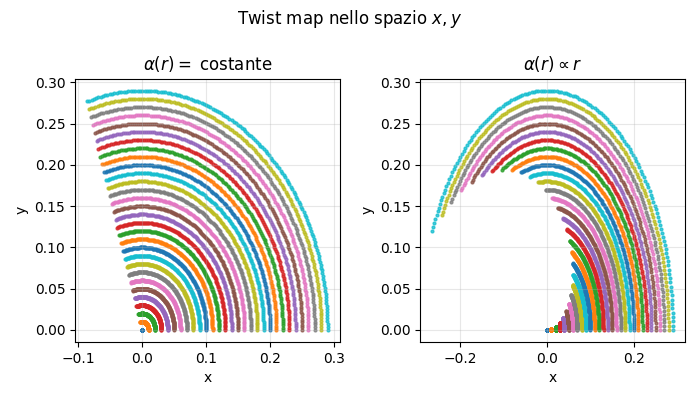
\includegraphics[width=0.45\textwidth]{figures/18_twist_tetha_r.png}
	\caption{\scriptsize Twist map nello spazio $x, y$, le condizioni iniziali utilizzate sono $\theta_0 = 0$. Per $r_0$ sono stati selezionati diversi valori tra $0$ e $0.3$ che danno origine alle curve rotanti (un colore corrisponde alla singola traiettoria, dopo il celeste la mappa di colori si ripete).}
        \label{fig:-figures-18_twist_tetha_r-png}
    \end{figure}
\end{exmp}
\noindent
\begin{exmp}[Twist map in cartesiane]
    Un esempio di Twist map in coordinate cartesiane è:
    \[
        \begin{cases}
            x_{i+1}=x_i+y_i\\
	    y_{i+1}=y_i
        \end{cases}
    \] 
    Notiamo che la struttura delle equazioni è identica al caso precedente (in coordinate polari).\\
    Questa mappa è area preserving, infatti:
    \[
        \begin{pmatrix} x_{i+1} \\ y_{i+1} \end{pmatrix} =
	\begin{pmatrix} 
	    1 & 1 \\
	    0 & 1
	\end{pmatrix} 
	\begin{pmatrix} x_i \\ y_i \end{pmatrix} 
    .\] 
    Partendo con dei punti aventi tutti la stessa coordinata $x$ si osserva che, per iterate successive, i punti con la $y$ maggiore vengono mandati in $x$ maggiori rispetto a quelli con una $x$ minore. La coordinata $y$ resta invece inalterata.\\
    Abbiamo quindi una rotazione $+$ dilatazione nello spazio $x,y$: una Twist map.
\end{exmp}
\noindent
\clearpage

\section{Lezione 19}%
\label{sub:Lezione 19}
\subsection{Mappa di Henon}%
\label{sub:Mappa di Henon}
La mappa di Henon è stata al centro di numerose ricerche sui sistemi caotici e non lineari. Henon ebbe l'idea di modellizzare con questa mappa il moto degli oggetti celesti. Secondo il suo modello, per determinati parametri iniziali, il moto sfocia nel caos.\\
Costruiamo la mappa in due step, un primo step è un "twist" con un termine $-x^2$, chiamiamo questa trasformazione $T_1$:
\[
    T_1: \quad
    \begin{cases}
        x' = x_i\\
	y' = y_i-x_i^2
    \end{cases}
.\] 
Mentre il secondo step ($T_2$) è una rotazione del primo:
\[
    T_2: \quad
    \begin{pmatrix} x_{i+1} \\ y_{i+1} \end{pmatrix} =
    \begin{pmatrix} 
	\cos\alpha  &  - \sin\alpha  \\
	\sin\alpha  &  \cos\alpha
    \end{pmatrix} 
    \begin{pmatrix} x' \\ y' \end{pmatrix} 
.\] 
In conclusione abbiamo $T = T_1\cdot T_2$:
\[
    \begin{cases}
	x_{i+1} = x_i\cos\alpha-(y_i-x_i^2)\sin\alpha\\
	y_{i+1} = x_i\sin\alpha + (y_i-x_i^2)\cos\alpha
    \end{cases}
.\] 
\begin{figure}[H]
    \centering
    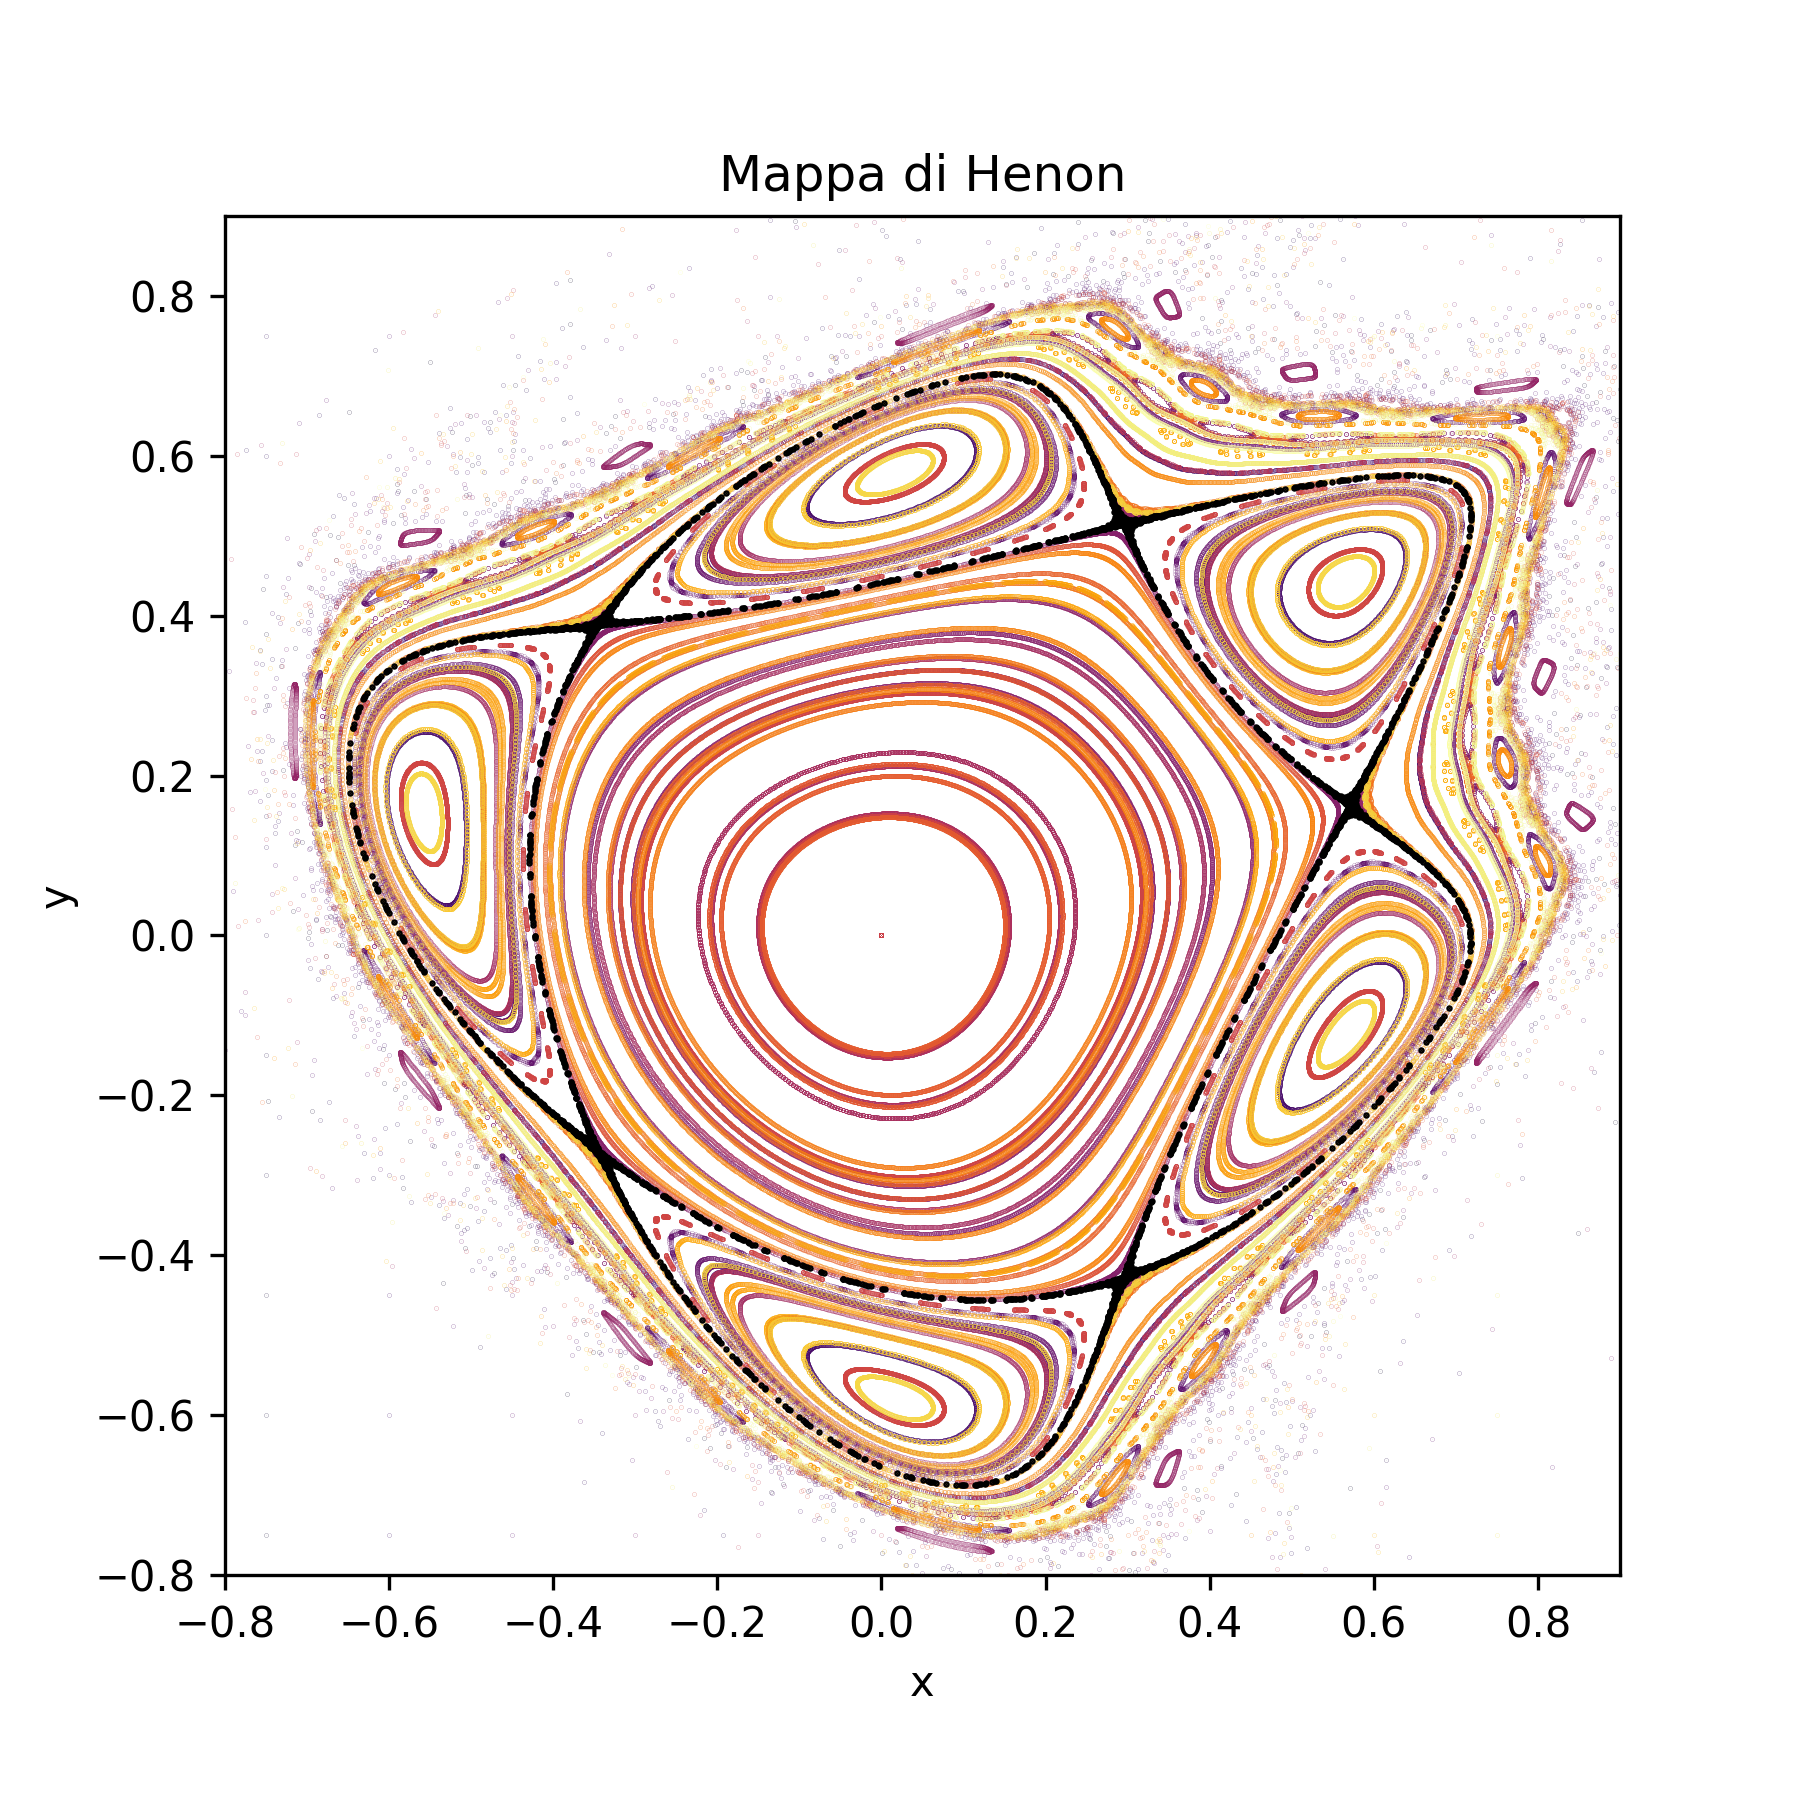
\includegraphics[width=0.5\textwidth]{figures/18_Henon_map.png}
    \caption{\scriptsize Mappa di Henon al variare dei parametri iniziali di $x$ e $y$ con $\alpha = 1.328$. Si è messa enfasi sulla traiettoria passante per il punto fisso (in nero). Notiamo come le traiettorie esterne sfocino già nel caos. Realizzata in Fortran e Python.\\
    In questa immagine c'è molto di più di quel che si vede, provando a valutare il moto negli intorni dei punti fissi appaiono strutture di vario genere, piccoli tori circondati da caos (provare a giocare con le condizioni iniziali per vedere).}
    \label{fig:figures-18_Henon_map-png}
\end{figure}
\noindent
Possiamo chiederci se questa mappa sia Area preserving. \\
Per quanto riguarda la rotazione $T_2$ non ci sono problemi, sappiamo che ogni rotazione ha un Jacobiano unitario. \\
La mappa $T_1$ invece (usiamo la notazione di sopra con $x', y'$):
\[
    \frac{\partial x'}{\partial x_i} = 1 \qquad \frac{\partial x'}{\partial y_{i}} = 0
\] 
\[
    \frac{\partial y'}{\partial x_i} = 0  \qquad  \frac{\partial y'}{\partial y_{i}} = 1
.\] 
Quindi abbiamo che il determinante della matrice delle derivate miste è unitario anche per $T_1$, di conseguenza la trasformazione è Area preserving e potrebbe essere attribuita ad una qualche Hamiltoniana. Quale Hamiltoniana genera questa mappa?
\subsection{Legare una mappa ad una Hamiltoniana}%
\label{sub:Legare una mappa ad una Hamiltoniana}
Prendiamo una Hamiltoniana del tipo:
\begin{equation}
    H(\vect{q}, \vect{p})=\sum_{}^{} \frac{1}{2}p_i^2 + V(\vect{q})
    \label{eq:19_H}
\end{equation}
\paragraph{L'integrazione di Eulero non è Area preserving}%
\label{par:Integrazione di Eulero}
Possiamo provare a discretizzare le equazioni del moto in questo modo:
\[
    \begin{cases}
        q_{i+1}=q_i + hp_i\\
	p_{i+1}=p_i - h \frac{\partial V}{\partial q_i} 
    \end{cases}
    \qquad
    h = \Delta t
.\] 
Possiamo scrivere la mappa in forma di matrice (in questo modo si isola lo Jacobiano):
\[
    \begin{pmatrix} q_{i+1}\\ p_{i+1} \end{pmatrix} =
    \begin{pmatrix} 
	1      & h \\
	- hV'' & 1
    \end{pmatrix} 
    \begin{pmatrix} q_i \\p_i \end{pmatrix}
.\] 
Dove la derivata seconda $V''$ appare perché si scrive:
\[
    \frac{\partial V}{\partial q_i} = \frac{\partial ^2V}{\partial q_i^2} \partial q_i
.\] 
Per rendere proporzionale a $q$ il termine con la derivata parziale di $V$. \\
Il determinante della trasformazione non è unitario:
\[
    \text{det} = 1 + h^2V'' \neq 1
.\] 
Quindi la mappa che si ottiene da una integrazione con Eulero non è area preserving. Integrando con questo metodo l'Hamiltoniana perderemo molto rapidamente le caratteristiche del nostro sistema fisico.
\paragraph{Eulero "a due step" è Area preserving}%
\label{par:Eulero "a due step" è Area preserving}
Prendiamo la seguente variante dell'integrazione con Eulero:
\[
    \begin{cases}
        q_{i+1}=q_i + hp_i\\
	p_{i+1}=p_i - h V_{i+1}
    \end{cases}
.\] 
In cui il termine $V'_{i+1}$ è la derivata del potenziale rispetto a $q_{i+1}$. \\
Così facendo il termine in basso a sinistra nello Jacobiano descritto sopra non c'è:
\[
    J = 
    \begin{pmatrix} 
	1 & h\\
	0 & 1
    \end{pmatrix} 
.\] 
Ed il determinante di questa matrice è 1: abbiamo una integrazione AP (Area preserving).\\
Il problema è che, a differenza delle equazioni agli incrementi di Eulero, questa integrazione non deriva direttamente dalle equazioni di Hamilton discretezzate dell'Hamiltoniana \ref{eq:19_H}. Da quale Hamiltoniana derivano?\\
Si può dimostrare che questa H deve esser della forma:
\begin{equation}
    H = \frac{p^2}{2} + h V(q)\delta(t-ih) \qquad i \in \mathbb{N}
    \label{eq:19_H_poincare}
\end{equation}
Per un tempo $h'$ abbiamo una equazione per particella libera ($H=p^2 /2$), tale Hamiltoniana si sa integrare (equazioni del moto lineari).
\[\begin{aligned}
    & q_{i+1}=q_i + hp_i\\
    & p_{i+1}=p_i
.\end{aligned}\]
Quindi lontano dalle $\delta$ abbiamo una specie di twist map.
Ai tempi $t=ih$ il nostro oggetto prende un colpo dal potenziale.\\
Immaginiamo di iniziare l'integrazione in un tempo tra $\left[ih, (i+1)h\right]$, in tal caso si ha per $q$ l'equazione scritta sopra, mentre per $p$ abbiamo una sorpresa:
\[
    \dot{p} = - \frac{\partial V}{\partial q}
.\] 
Se la integriamo nel tempo sopravvivono soltanto dei pezzi negli intorni di $(i+1)h$ (il tempo $ih$ è già passato):
\[
    p_{i+1} - p_i = -\int\limits_{(i+1)h-\epsilon}^{(i+1)h+\epsilon} V' dt  = - h V_{i+1}'
.\] 
Notiamo che si potrebbe anche invertire il ruolo di $p$ e $q$, effettuando prima il "calcio" e successivamente l'evoluzione:
\[\begin{aligned}
    & q_{i+1} = q_i + p_{i+1}h\\
    & p_{i+1} = p_i - V_i'h
.\end{aligned}\]
\paragraph{Analogia con le mappe di Poincare}%
\label{par:Analogia con le mappe di Poincare}
La questione del passaggio dall'Hamiltoninana di partenza ad una mappa (e viceversa) è quindi risolta? Cosa significa fisicamente risolvere per una Hamiltoniana come quella di equazione \ref{eq:19_H_poincare}?\\
Sorprendentemente signfica che stiamo studiando una mappa di Poincare: fissare degli istanti di "osservazione" del sistema con la $\delta$ significare fissare dei piani a tempi fissi nello spazio ($q,p,t$), esattamente quello che si fa con una mappa di Poincare.\\
Infatti fissare un piano di osservazione
\footnote{ad esempio $y=0$ come nell'esempio della lezione scorsa}
significa aspettare gli istanti in cui l'oggetto passerà nuovamente da tale piano, quindi è esattamente l'analogo di quello che stiamo facendo adesso.
\subsection{Introduzione alla mappa standard}%
\label{sub:Introduzione alla mappa standard}
La maggior parte degli studi sul caos è stato effettuato sulla mappa standard. Tale mappa ha la seguente struttura:
\begin{redbox}{Mappa standard}
 \[\begin{aligned}
    & q_{i+1} = q_i + p_{i+1}\\
    & p_{i+1} = p_i + \frac{k}{2\pi}\sin (2\pi q_i)
.\end{aligned}\]   
\end{redbox}
\noindent
In cui si sceglie mod($q$)=mod($p$)=1
\footnote{Su wikipedia si dice che solitamente $p, q$ sono presi modulo $2\pi$ (perché non si divide per $2\pi$ l'incremento con $k$), quindi si divide $p$ e $q$ per $2\pi$ ogni step e se ne prende il resto.Nel caso di modulo 1 il resto è il numero stesso.}
.\\
Notiamo anche che il potenziale in questione è quello di un pendolo.
\begin{figure}[H]
    \centering
    \includegraphics[width=0.5\textwidth]{figures/19_standard_map.png}
    \caption{\scriptsize Mappa standard integrata con $k=0.97$. Si nota la presenza di strutture che ricordano tori invarianti, in altre zone è invece evidente la presenza di caos.}
    \label{fig:figures-19_standard_map-png}
\end{figure}
\noindent
Questa mappa è sicuramente Hamiltoniana, infatti si ha uno Jacobiano:
\[
     M = 
     \begin{pmatrix}
	 1 & 0 \\
	 k \cos(2\pi q_i) & 1
     \end{pmatrix} 
.\] 
Abbiamo un termine non lineare in basso a sinistra, tuttavia ai fini del determinante questo non ha importanza.
\subsection{Studio dei punti fissi per un mappa Hamiltoninana}%
\label{sub:Studio dei punti fissi per un mappa Hamiltoninana}
Definiamo la mappa come la trasformazione $T$, cerchiamo di capire cosa avviene nella mappa nei punti $x^*$ tali per cui:
\[
    x^* = T(x^*)
.\] 
In particolare ci concentriamo su un intorno di questi cercando di linearizzare il problema:
\[
    \vect{x} = \vect{x}^* + \delta\vect{x}
.\] 
\[\begin{aligned}
    \implies  & \vect{x}_{n+1} = \vect{x}^* + \delta\vect{x}_{n+1} = T(\vect{x}^* + \delta\vect{x}_n) = \\
	      & \simeq T(\vect{x}^*) + \left.\frac{\partial T}{\partial \vect{x}} \right|_{\vect{x}^*}\delta\vect{x}_n
.\end{aligned}\]
Abbiamo quindi che il comportamento al punto fisso è determinato dalla matrice delle derivate miste:
\[
    \delta\vect{x}_{n+1} = \left.\frac{\partial T}{\partial \vect{x}} \right|_{\vect{x}^*}\delta\vect{x}_n \delta\vect{x}_n
.\] 
Esplicitamente:
\[
    \begin{pmatrix} \delta x_{n+1} \\ \\ \delta y_{n+1} \end{pmatrix} = 
    \begin{pmatrix} 
	\frac{\partial T_x}{\partial x} && \frac{\partial T_x}{\partial y} \\
					&&\\
	\frac{\partial T_y}{\partial y} && \frac{\partial T_y}{\partial y} 
    \end{pmatrix} 
    \begin{pmatrix} \delta x_{n} \\ \\ \delta y_{n} \end{pmatrix} 
.\] 
Essendo la mappa per ipotesi Hamiltoninana si ha che matrice al centro (che chiamiamo $M$) ha determinante unitario, gli autovalori di questa matrice possono essere ricavati tramite l'equazione secolare:
\[\begin{aligned}
    \text{det}(M-\lambda\mathbb{I})=&\lambda^2-\lambda\text{tr}(M)+\text{det}(M) = \\
    =&\lambda^2-\lambda\text{tr}(M)+1
.\end{aligned}\]
\[
    \lambda_{\pm} = \frac{\text{tr}(M)\pm\sqrt{(\text{tr}(M))^2-4}}{2}
.\] 
ci sono allora due possibilità per gli autovalori:
\begin{itemize}
    \item $\left|\text{tr}(M)\right|<2$: autovalori complessi coniugati.
    \item $\left|\text{tr}(M)\right|>2$: autovalori reali.
\end{itemize}
Il fatto che il determinante di $M$ sia unitario comporta anche che il prodotto tra i due autovalori faccia 1:
\[
    \lambda_+\cdot \lambda_- = 1
.\] 
Quindi possiamo definire $\lambda_+ = \lambda$, di conseguenza:
\[
    \lambda_+ = \lambda  \qquad \lambda_- = \frac{1}{\lambda}
.\] 
\paragraph{Autovalori reali}%
\label{par:Autovalori reali}
Consideriamo il caso in cui gli autovalori sono reali con autovettori corrispondenti $\vect{\omega}$, l'evoluzione di questi vettori avrà la seguente forma per definizione:
\[
    \delta\vect{\omega}_{n+1} = 
    \begin{pmatrix} 
	\lambda  & 0 \\
	0 & 1 /\lambda
    \end{pmatrix} 
    \delta\vect{\omega}_n
.\] 
Quindi l'evoluzione degli autovettori si distingue in due casi:
\begin{enumerate}
    \item $\lambda > 0$:
	Allora abbiamo le due evoluzioni per gli autovettori:
	\[
	    \omega^{(+)}_n = \lambda^n \omega_0; \qquad \omega^{(-)}_n = \left(\frac{1}{\lambda}\right)^n \omega_0
	.\] 
	Quindi in una direzione abbiamo una espansione, nell'altra una contrazione.
    \item $\lambda < 0$: In questo caso si ha l'analogo del caso precedente però ad ogni step gli assi invertono la loro direzione
	\[
	    \omega^{(+)}_n = (-1)^n\lambda^n \omega_0; \qquad \omega^{(-)}_n = (-1)^n\left(\frac{1}{\lambda}\right)^n \omega_0
	.\] 
\end{enumerate}
Nel caso (1) possiamo anche dire qualcosa in più sul nostro sistema: scriviamo l'equazione di $\omega_n$ in termini di esponenziali
\[
    \omega_n = \omega_0 \exp (n\ln\lambda)
.\] 
In questa equazione il termine $n$ gioca il ruolo di un tempo, in questo modo si scopre che la scala di evoluzione del sistema $\tau$ è:
\[
    \tau\sim \frac{1}{\ln\lambda}
.\] 
Questa è la scala con la quale gli oggetti si allontanano/collassano su un punto fisso.\\
Questo studio dei punti fissi ci serve per capire cosa succede in un sistema quando si rompe il teorema KAM.
\subsection{Caos e rottura del teorema KAM}%
\label{sub:Caos e rottura del teorema KAM}
Prendiamo la seguente mappa in coordinate azione angolo:
\[\begin{aligned}
    & \varphi_{n+1} = \varphi_n + \frac{\partial }{\partial I_{n+1}} S_0(I_{n+1})\\
    & I_{n+1} = I_n
.\end{aligned}\]
Questa è molto simile ad una Twist map. A destra della prima equazione abbiamo il termine $\partial_{I_{n+1}}S_0$, questo può essere associato al rapporto tra le frequenze della Hamiltoniana predetto in generale per le twist map nella lezione precedente.
\[
    \partial_{I_{n+1}}S_0 \sim 2\pi  \frac{\omega_1}{\omega_2}
.\] 
Nel seguito supponiamo che il termine $\alpha(I) = \omega_1 /\omega_2(I)$ proporzionale a $I$, quindi abbiamo una specie di twist map come nella seconda figura di Figura \ref{fig:-figures-18_twist_tetha_r-png}.\\
Il teorema KAM ci assicura che i primi tori che si rompono sono quelli per il quale il rapporto $\omega_1 /\omega_2$ è un numero razionale. \\
Prendiamo una situazione in cui alcuni tori previsti dal teorema KAM sono preservati mentre si rompe un singolo toro di quelli razionali, cerchiamo di capire cosa si vede nello spazio delle fasi in questo caso.
L'idea per far questo è sempre quella di scrivere una teoria perturbativa su $S$:
\[\begin{aligned}
     & \varphi_{n+1} = \varphi_n + \frac{\partial }{\partial I_{n+1}} S_0 + \epsilon\frac{\partial }{\partial I_{n+1}} S_1(I_{n+1}, \varphi_n)\\
     & I_{n+1} = I_n + \epsilon\frac{\partial }{\partial \phi_{n}} S_1(I_{n+1}, \varphi_n) 
.\end{aligned}\]
Come sappiamo sono i termini perturbativi introdotti in queste equazioni a rompere il toro. Possiamo vedere cosa avviene alle curve che si rompono.\\
Partiamo dai tori imperturbati, questi nello spazio $I, \varphi$ faranno delle circonferenze poiché $I$ si conserva. \\
Prendiamo allora 3 di questi tori aventi $I$ crescente (che chiamiamo $C_+, C, C_-$), questi formeranno 3 circonferenze concentriche come in figura \ref{fig:19_tori}. \\
Scegliamo il toro centrale $C$ tale che la sua frequenza sia razionale, quindi ci aspettiamo che sia un toro che si rompe prima degli altri due limitrofi.\\
Si effettua un cambio di sistema di riferimento in modo tale da rendere i punti del toro centrale fermi, gli altri due tori avranno la caratteristica (nel nuovo sistema) di ruotare uno in senso orario e l'altro in senso antiorario poiché $\omega\propto I$.
\begin{figure}[H]
    \centering
    \incfig{19_tori}
    \caption{\scriptsize Cambio di sistema di riferimento, i punti del toro al centro sono fermi poiché siamo in un sistema rotante con la $\omega$ di quel toro. \\
    Il toro più grande aveva una $\omega$ più grande, il toro più piccolo invece una $\omega$ più piccola rispetto al centrale. Per questo motivo il primo gira in senso orario ed il secondo in senso antiorario dopo la trasformazione.}
    \label{fig:19_tori}
\end{figure}
\noindent
A questo punto possiamo accendere la perturbazione (si reinserisce nelle equazioni i termini con $\epsilon$). In questo modo i nuovi tori $C_{-,\epsilon}$, $C_{+, \epsilon}$ subiscono una piccola perturbazione rispetto alle loro posizioni iniziali, il toro centrale $C$ invece si rompe e cessa di esistere.
\begin{figure}[H]
    \centering
    \incfig{19_tori_rotto}
    \caption{\scriptsize Il toro $C$ si rompe in seguito alla accensione della perturbazione, ciò che resta di lui è l'alone nero al centro a rappresentare il caos. In magenta abbiamo la varietà di punti fermi tra i due tori che deve esistere necessariamente per la continuità di $\varphi$ ed $I$.}
    \label{fig:19_tori_rotto}
\end{figure}
\noindent
Dopo la rottura del toro $C$  tra i due tori dovrà necessariamente esistere una varietà di punti aventi $\omega =0$. Questo perché il toro esterno ed il toro interno hanno $\omega$  di segno opposto in questo sistema, tracciando una linea che passa per i due tori necessariamente deve esistere un punto in mezzo che annulla la $\omega$. \\
Chiamando la mappa $T_{\epsilon}$ abbiamo che, per i punti appartenenti alla varietà rimasta fissa:
\[
    \varphi^* = T_{\epsilon}(\varphi^*)
.\] 
Sicuramente la varietà rossa dei punti fermi non è invariante, quindi evolverà negli step successivi. L'unico modo per cui può evolvere questa varietà è quello di variare la componente radiale poiché quella angolare è fissata per definizione di questa curva. \\
La cosa importante è che i punti fissi dovranno appartenere per ogni step a tale varietà, per tali punti deve valere sempre:
\[
    I^* = T_{\epsilon}(I^*)
.\] 
\begin{figure}[H]
    \centering
    \incfig{19_tori_step}
    \caption{\scriptsize Andamento della varietà con i punti aventi $\omega =0$ al variare degli step della mappa, nella prima figura in alto a sinistra si mostra la mappa imperturbata, in tal caso la varietà dei punti fermi corrisponde con il toro invariante per costruzione.\\
    Le due figure successive corrispondono all'aver acceso la perturbazione, le curve magenta e blu pertanto non sono tori poiché in questa zona c'è il caos. In nero sono presenti i punti fissi.}
    \label{fig:19_tori_step}
\end{figure}
\noindent
La cosa interessante da capire è la struttura dei punti fissi, questa ci dirà in che modo i tori si stanno spaccando. \\
Guardiamo da vicino una zona della figura precedente: 
\begin{figure}[H]
    \centering
    \incfig{19_tori_ingrandimento}
    \caption{\scriptsize Ingrandimento su zona con punti fissi, le frecce indicano la direzione di variazione della varietà fissa o isocrona.}
    \label{fig:19_tori_ingrandimento}
\end{figure}
\noindent
Possiamo vedere che tra la varietà del primo step e quella del secondo i punti devono necessariamente avvicinarsi/allontanarsi dal punto fisso. Questo è dovuto al fatto che $\omega \propto I$, quindi per passare da zone con $I$ maggiore/minore c'è bisogno di accelerare/rallentare.\\
Questa particolarità ci dice che i punti fissi sono un alternanza di punti iperbolici ed ellittici. Tutti questi punti fissi vivono tra i due tori quasi conservati $C_{\pm, \epsilon}$.\\
Prendiamo in considerazione il punto iperbolico in figura (quello in basso) e cerchiamo di capire cosa viene in un suo intorno.\\
Sappiamo che un punto iperbolico è caratterizzato da due curve instabili (che si allontanano esponenzialmente dal punto) e da due curve stabili (che cadono esponenzialmente nel punto), tali curve vengono chiamate Manifold.
\begin{figure}[H]
    \centering
    \incfig{19_stab_instab}
    \caption{\scriptsize Curve stabili ed instabili per il punto iperbolico. Notiamo che non devono necessariamente coincidere con le curve isocrone, l'importante è che siano consistenti con le direzioni di figura \ref{fig:19_tori_ingrandimento}.\\
    Dobbiamo anche precisare che le curve colorate siano delle varietà stabili mentre le linee con le frecce sono delle possibili mappe di Poincare.}
    \label{fig:19_stab_instab}
\end{figure}
\noindent
Può succedere che le due curve nere, nelle vicinanze del punto fisso, si incrocino in un punto (diverso dal punto iperbolico). L'intersezione è quasi inevitabile visto che il punto iperbolico è schiacciato tra due tori: i manifold (curve nere) sono costretti a "piegarsi" prima o poi per non oltrepassare il toro.
\begin{figure}[H]
    \centering
    \incfig{19_intersezione}
    \caption{\scriptsize Intersezione dei Manifold nei pressi di un punto fisso.}
    \label{fig:19_intersezione}
\end{figure}
\noindent
Immaginiamo adesso di far evolvere le traiettorie nella direzione del punto di incrocio del manifold. Iterando la mappa si avrà una situazione del tipo:
\begin{figure}[H]
    \centering
    \incfig{19_itero_fisso}
    \caption{\scriptsize Iterazioni della mappa per punti attorno al punto di incrocio dei manifold.}
    \label{fig:19_itero_fisso}
\end{figure}
\noindent
Adesso se si prova ad iterare la mappa per il punto $P$  si ottiene un paradosso: l'iterazione $T(P)$  dovrebbe stare davanti sia a $T(x)$  che a $T(x')$.
L'unica situazione possibile è che i manifold si incrocino ancora in un punto $T(P)$.
\begin{figure}[H]
    \centering
    \incfig{19_manifold_incrocio1}
    \caption{\scriptsize Iterazione della mappa nei pressi del punto di intersezione dei manifold: si genera un ulteriore punto di intersezione dei manifold.}
    \label{fig:19_manifold_incrocio1}
\end{figure}
\noindent
Abbiamo quindi generato una zona chiusa tra le intersezioni dei manifold di area $A$.
Per una iterazione successiva il punto $T(P)$ dovrà andare in un punto $T^2(P)$ che è ancora un altra intersezione di manifold, quindi le due curve nere si intersecheranno ancora, generando un altra superficie separata di area $A$ (la stessa di prima perché la mappa è area preserving).\\
Adesso dobbiamo ricordare che i manifold si allontanano/avvicinano esponenzialmente al punto fisso. Possiamo notare nella figura \ref{fig:19_manifold_incrocio1} che al momento della prima iterata della mappa (quando creo $T(P)$) il manifold uscente ha fatto più strada del manifold entrante.\\
Tenendo di conto di questo nelle iterate successive lo spostamento dal punto $T(P)$ per il punto $T^2(P)$ sarà maggiore nella direzione di allontanamento dal punto fisso rispetto a quella di avvicinamento.\\
Come conseguenza oltre a preservare l'area le curve generate saranno sempre più allungate e schiacciate come in figura %\ref{}
\begin{figure}[H]
    \centering
    \incfig{19_itero2}
    \caption{\scriptsize Seconda iterazione della mappa: si genera un secondo punto di intersezione. \\ Notiamo come la seconda "area" generata sia stata rappresentata piegata, questo perché i manifold sono linee separatrici dello spazio delle fasi: non si possono attraversare.}
    \label{fig:19_itero2}
\end{figure}
\noindent
Iterando la procedura ancora e ancora nello spazio delle fasi succederà un gran casino, i manifold oscilleranno su loro stessi generando altre intersezioni dal quale potrebbero nascere altre oscillazioni\ldots è caos.\\
Queste strutture oscillanti possono generarsi da uno stesso punto fisso (\textbf{strutture omocliniche}) oppure a partire dalla intersezione di manifold provenienti da punti fissi diversi (\textbf{strutture eterocliniche})
\subsubsection{Strutture autosimilari nei punti ellittici}%
\label{subsub:Strutture autosimilari nei punti ellittici}
Nei pressi dei punti ellittici invece abbiamo delle isole invarianti, infatti all'interno di queste strutture non può penetrare il caos generatosi attorno ai punti iperbolici circostanti. \\
In pratica si ha che "ingrandendo" la zona di un punto ellittico si osserva una struttura del tutto analoga a quella originale: anche all'interno dell'isola invariante ci saranno punti fissi iperbolici ed ellittici a formare quindi una struttura self similare.
\clearpage

\section{Lezione 20}%
\label{sub:Lezione 20}
Possiamo suddividere il caos in due grandi categorie:
\begin{itemize}
    \item Caos Globale: invade lo spazio delle fasi su tutte le scale.
    \item Caos locale: limitato ad una regione dello spazio delle fasi.
\end{itemize}
\subsection{Indicatori di caos locale: esponenti di Lyapunov}%
\label{sub:Indicatori di caos locale: esponenti di Lyapanov}
Intuitivamente una regione è localmente caotica se le traiettorie con condizioni iniziali "vicine" si allontanano "rapidamente" (ed in modo esponenziale).\\
Ci si aspetta che la differenza tra due traiettorie inizialmente vicine venga amplificata esponenzialmente.\\
Quindi possiamo prendere il sistema da studiare, far evolvere due traiettorie con condizioni iniziali vicine e vedere in che modo si allontanano le traiettorie: questa è l'idea alla base degli esponenti di Lyapunov.\\
Definiamo la mappa di partenza come:
\[
    \vect{x}_{n+1} = F(\vect{x}_n)
.\] 
Questa mappa genererà una traiettoria $\vect{x}^{(t)}$. Prendiamo un punto $x_n$ sulla traiettoria $\vect{x}^{(t)}$, vi aggiungiamo una piccola perturbazione $\delta\vect{x}_n$ e andiamo a vedere come evolve la traiettoria.
\[
    \vect{x}_{n+1} + \delta\vect{x}_{n+1} = F(\vect{x}_n) + \frac{\partial F_n}{\partial \vect{x}_n}  \delta\vect{x}_n
.\] 
Quindi si ottiene una evoluzione delle variazioni $\delta\vect{x}_n$ secondo la mappa $F$. Possiamo definire allora la \textbf{mappa tangente} come:
\[
    \delta\vect{x}_{n+1} = \left.\frac{\partial F}{\partial \vect{x}} \right|_{\vect{x}^{(t)}}\delta\vect{x}_n
.\] 
Quindi per ottenere la mappa tangente ci si muove lungo la traiettoria $\vect{x}^{(t)}$  solo che ogni volta si valuta la variazione $\delta\vect{x}_{n+1}$.
\begin{exmp}[Mappa standard]
    \[\begin{aligned}
	&q_{n+1} = q_n + p_{n+1}\\
	&p_{n+1} = p_n + \frac{k}{2\pi}\cos ( 2\pi  q_n)
    .\end{aligned}\]
    In questo caso possiamo fare il seguente cambio di variabili:
    \[\begin{aligned}
	& q_n \to q_n + \delta q_n\\
	& p_n \to p_n + \delta p_n
    .\end{aligned}\]
    A questo punto dobbiamo derivare la mappa rispetto a $q_n$ e $p_n$, in tal modo otteniamo la mappa tangente:
    \[\begin{aligned}
	& \delta q_{n+1} = \delta q_n \\
	& \delta p_{n+1} = \delta p_n - k \sin (2\pi q_n)\delta q_n
    .\end{aligned}\]
    Possiamo scriverla anche in forma di matrice:
    \[
        \begin{pmatrix} \delta q_{n+1} \\ \delta p_{n+1} \end{pmatrix} =
	\begin{pmatrix} 
	    1 & 0 \\
	    -k \sin (2\pi q_n) & 1
	\end{pmatrix} 
	\begin{pmatrix} \delta q_n \\ \delta p_n \end{pmatrix} 
    .\] 
\end{exmp}
\noindent
Quindi per ogni punto della traiettoria $\vect{x}^{(t)}$ abbiamo un set di autovalori ed autovettori che diagonalizzano la mappa tangente ($M$).\\
Ipotizziamo di fare $n$ step della nostra mappa $F$, la mappa tangente varia sotto iterazione nel seguente modo:
\[
    \left(M\right)^{(t)}_n = M(\vect{x}^{(t)}_n)M(\vect{x}^{(t)}_{n-1})\ldots M(\vect{x}^{(t)}_0)
.\] 
Quindi se abbiamo diagonalizzato la mappa tangente alla fine avremo semplicemente che:
\[
    \left(M\right)^{(t)}_n \sim \lambda^n \sim e^{n\ln\lambda}
.\] 
Quindi a questo punto, come già fatto nella lezione precedente, possiamo interpretare $n$ come un tempo e $(\ln\lambda)^{-1}$ il tempo caratteristico del sistema.\\
Notiamo anche che il segno di $\ln\lambda$ decide se le nostre traiettorie divergeranno o rimarranno legate alla traiettoria originale.\\
Visto che vogliamo un oggetto locale e che, alla fine, cerchiamo una quantità che ci dia un "resoconto" di quello che è avvenuto durante la traiettoria consideriamo la radice $n$-esima dell'ultima espressione:
\[
    (M)_n \equiv \left((M^{(t)}_n)\right)^{1/n}
.\] 
Se $D$ è la dimensione del sistema questa equazione avrà $D$ autovalori e $D$ autovettori. L'insieme dei $D$ autovalori si chiama \textbf{Spettro di Lyapunov}: $\sigma_i$.
\[
    \sigma_i = \lim_{N \to \infty} \ln\left|\lambda_i(N)\right| \qquad i = 1, \ldots, D
.\] 
\subsubsection{Spettro di Lyapunov per mappe Hamiltoninane}%
\label{subsub:Spettro di Lyapanov per mappe Hamiltoninane}
Nel caso di un sistema dinamico continuo come quello derivante da una Hamiltoniana in generale si avranno $2n$ esponenti $\sigma$: $n$ per le $p$ ed $n$ per le $q$.\\
In particolare, essendo il sistema Hamiltoninano, devono valere le seguenti proprietà:
\begin{itemize}
    \item $\sum_{}^{} \sigma_i = 0$ per la conservazione del volume nello spazio delle fasi.\\
	Infatti le $\sigma$ ci dicono quanto si espande/contrae il sistema. Se si conserva il volume la somma di tutte queste trasformazioni sarà nulla.
    \item Visto che le variabili $p, q$ sono coniugate si avrà che le $\sigma$ andranno "a coppie": se $\sigma_j=2$ allora esiste $\sigma_{\overline{j}}=-2$. La regola generale si scrive come:
	\begin{equation}
	    \sigma_i = - \sigma_{2n-i+1}
	    \label{eq:20_sigma}
	\end{equation}
	Può sembrare una proprietà non banale, in realtà anch'essa deriva da $dpdq = $ cost.\\
	Come conseguenza di questa regola esisteranno necessariamente due $\sigma$ nulle. \\
	Questo deriva dal fatto che l'Hamiltoniana conserva l'energia, quindi esisterà almeno una curva sul quale giace la traiettoria ad energia zero. Per tale traiettoria si avrà un $\sigma$ nullo, quindi per la \ref{eq:20_sigma} dovranno esistere due autovalori nulli.
\end{itemize}
\subsection{Mappa tangente nel caso unidimensionale}%
\label{sub:Mappa tangente nel caso unidimensionale}
Prendiamo una mappa unidimensionale del seguente tipo:
\[
    x_{n+1} = f(x_n)
.\] 
Quindi la mappa tangente sarà così fatta:
\[
    \delta x_{n+1} = f'\delta x_n = \prod_{J=0}^{} f'_J \delta x_0 
.\] 
Considerando che deve valere: 
\[
    \delta x_{n+1} = e^{N\sigma}\delta x_n
.\] 
L'esponente di Lyapunov per il sistema è:
\[
    \sigma  = \frac{1}{N} \ln\left[\prod_{J=0}^{} f'_J \right] =
    \frac{1}{N}\sum_{J}^{} \ln\left|f'_J\right|
.\]
\begin{exmp}[Esempio unidimensionale]
    \[
        x_{n+1}=2x_n
	\implies
        f'_J = 2
    .\] 
    \[
	\sigma  = \frac{1}{N}\sum_{J}^{} \ln (2) = \ln 2
    .\] 
    Quindi essendo $\sigma >0$ mi aspetto che le traiettorie del moto divergano esponenzialmente al variare dei parametri iniziali, con un tempo tipico dato da $1 /\sigma$.
\end{exmp}
\subsection{Mappa logistica}%
\label{sub:Mappa logistica}
Prendiamo un'altra mappa unidimensionale molto famosa: la mappa logistica.
\[
    x_{n+1}=4\lambda x_n (1-x_n) \qquad 0\le x_n\le 1
.\] 
Il massimo della mappa logistica è per $x = 1 /2$. Ponendo come condizione iniziale $x_0 = 0.5$ ci si accorge che, per avere un moto vincolato tra $\left[0,1\right]$ deve essere $0<\lambda <1$.\\
In questo caso la mappa tangente è:
\begin{equation}
    \delta x_{n+1} = 4\lambda(1-2x_n)\delta x_n
    \label{eq:20_tangente_log}
\end{equation}
Prendiamo ad esempio il caso $\lambda = 3 /4$, possiamo visualizzare la mappa nel piano $x_n$  vs $x_{n+1}$ in figura \ref{fig:figures-20_mappa_logistica_0-75-png}.
\begin{figure}[h]
    \centering
    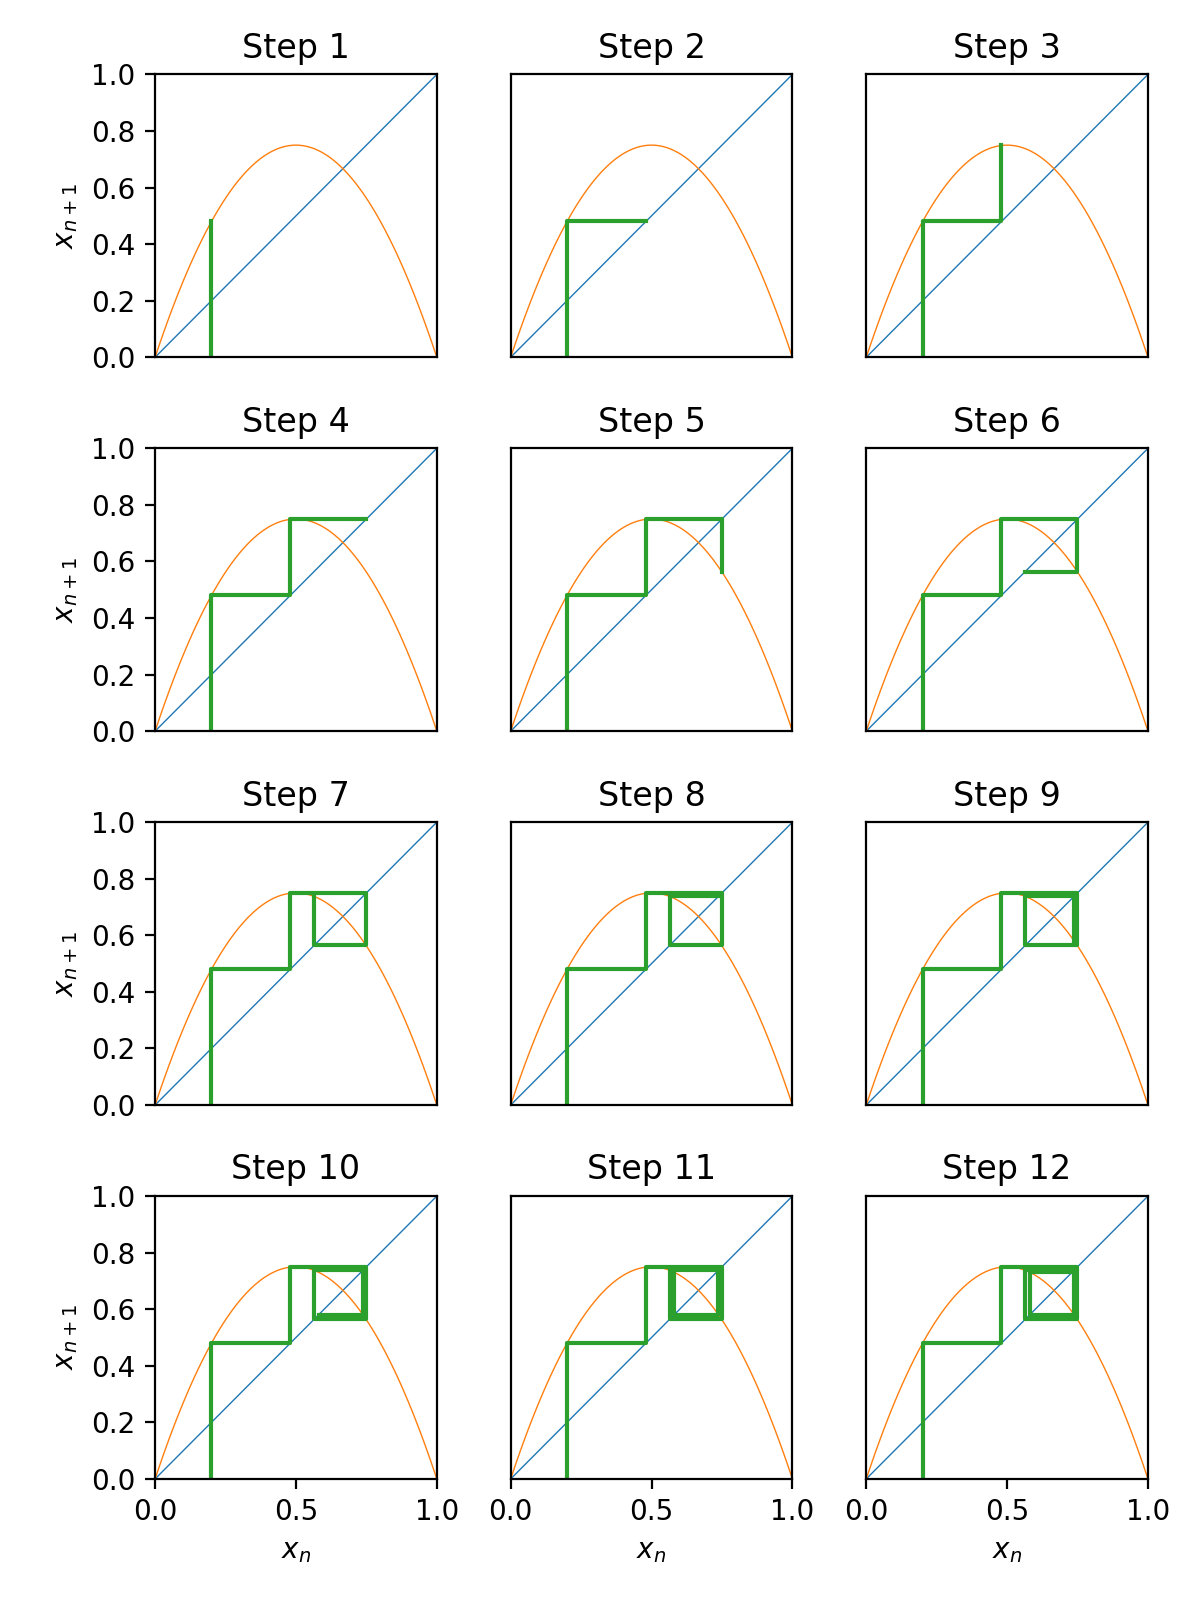
\includegraphics[width=0.45\textwidth]{figures/20_mappa_logistica_0.75.png}
    \caption{\scriptsize Mappa logistica nello spazio $x_n, x_{n+1}$. La linea verde rappresenta la retta tale per cui $x_n = x_{n+1}$, quella arancione invece è il grafico della mappa stessa. \\
    Per costruire gli step è sufficiente proiettare il valore $x_n$ sulla parabola arancione (applicare la mappa) e proiettare $x_{n+1}$ sulla retta verde (mandare $x_{n}$ in $x_{n+1}$). Questi due step vengono ripetuti e rappresentano l'evoluzione della traiettoria.}
    \label{fig:figures-20_mappa_logistica_0-75-png}
\end{figure}
\noindent
Facendo riferimento alla \ref{fig:figures-20_mappa_logistica_0-75-png} i punti in cui la parabola arancione incrocia la retta verde sono punti fissi della mappa. Possiamo notare che una mappa logistica ha due punti fissi: l'origine e quello in alto nel quale la traiettoria sembra girare attorno.
\subsubsection{Stabilità dei punti fissi della mappa logistica}%
\label{subsub:Stabilità dei punti fissi della mappa logistica}
La mappa tangente (\ref{eq:20_tangente_log}) ci aiuta nella valutazione della stabilità dei punti fissi.\\
Partiamo dal punto fisso nell'origine: ponendo $x_n = 0$ nella equazione della mappa tangente:
\[
    \delta x_{n+1} = 4\lambda\delta x_n
.\] 
Quindi se $4\lambda > 1$ l'origine è un punto instabile, viceversa se $4\lambda <1$ l'origine è un punto stabile.\\
L'altro punto fisso si ha imponendo nella equazione della mappa $x_{n+1}=x_n$:
\[
    1 = 4\lambda (1-x_n)
.\] 
\[
    x_n = 1 - \frac{1}{4\lambda}
.\] 
Notiamo che questo oggetto deve essere ancora compreso tra $0$ e $1$, per questo è necessario imporre un vincolo su $\lambda$:
\[
    0 < 1-\frac{1}{4\lambda}<1
.\] 
Quindi deve essere $\lambda >1 /4$.
Inserendo il valore del secondo punto fisso $x_n$ nella mappa tangente:
\[
    \delta x_{n+1}= 4\lambda (1 -2 + \frac{1}{2\lambda})\delta x_n = (-4\lambda  + 2)\delta x_n
.\] 
Quindi ora abbiamo che se $\left|2 - 4\lambda\right| < 1 (> 1)$ abbiamo la (in)stabilità di questo secondo punto fisso.\\
Mettendo tutto insieme:
\begin{itemize}
    \item $\lambda<1 /4$ il punto fisso non c'è.
    \item $1 /4 <\lambda  < 3 /4$ punto fisso stabile.
    \item $3 /4 <\lambda <1$ punto fisso instabile.
\end{itemize}
Possiamo anche raffigurare le traiettorie della mappa al variare del parametro $\lambda$, si ottengono delle immagini molto particolari (figura \ref{fig:figures-20_mappa_logistica_lambda-png}).
\begin{figure}[h]
    \centering
    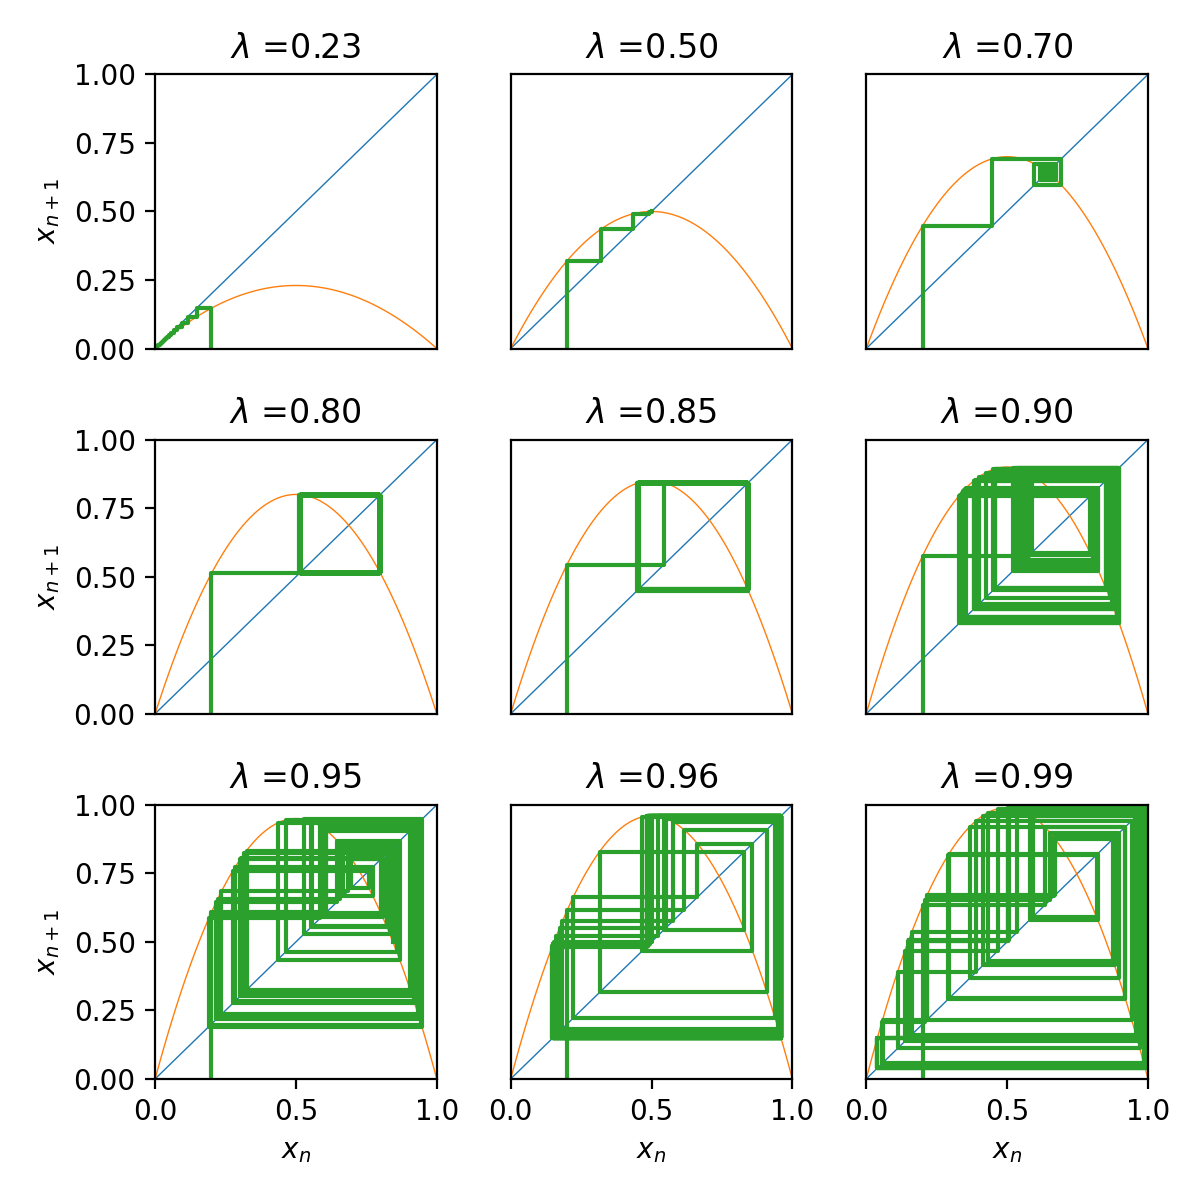
\includegraphics[width=0.45\textwidth]{figures/20_mappa_logistica_lambda.png}
    \caption{\scriptsize Andamento delle prime 100 iterazioni per la mappa logistica al variare di $\lambda$. Dopo un certo valore di $\lambda$ maggiore di $3 /4$ subentra il caos nelle traiettorie.}
    \label{fig:figures-20_mappa_logistica_lambda-png}
\end{figure}
\noindent
Notiamo come, iterando la mappa, se non si sviluppa il caos le traiettorie prediligono pochi punti sul quale adagiarsi. Due dei quali sono (per $\lambda  < 3 /4$) i due punti fissi discussi sopra. \\
Possiamo vedere il subentrare del caos anche con il grafico di Feigenbuam in figura \ref{fig:figures-20_mappa_logistica_-Feigenbuam-png}.
\begin{figure}[H]
    \centering
    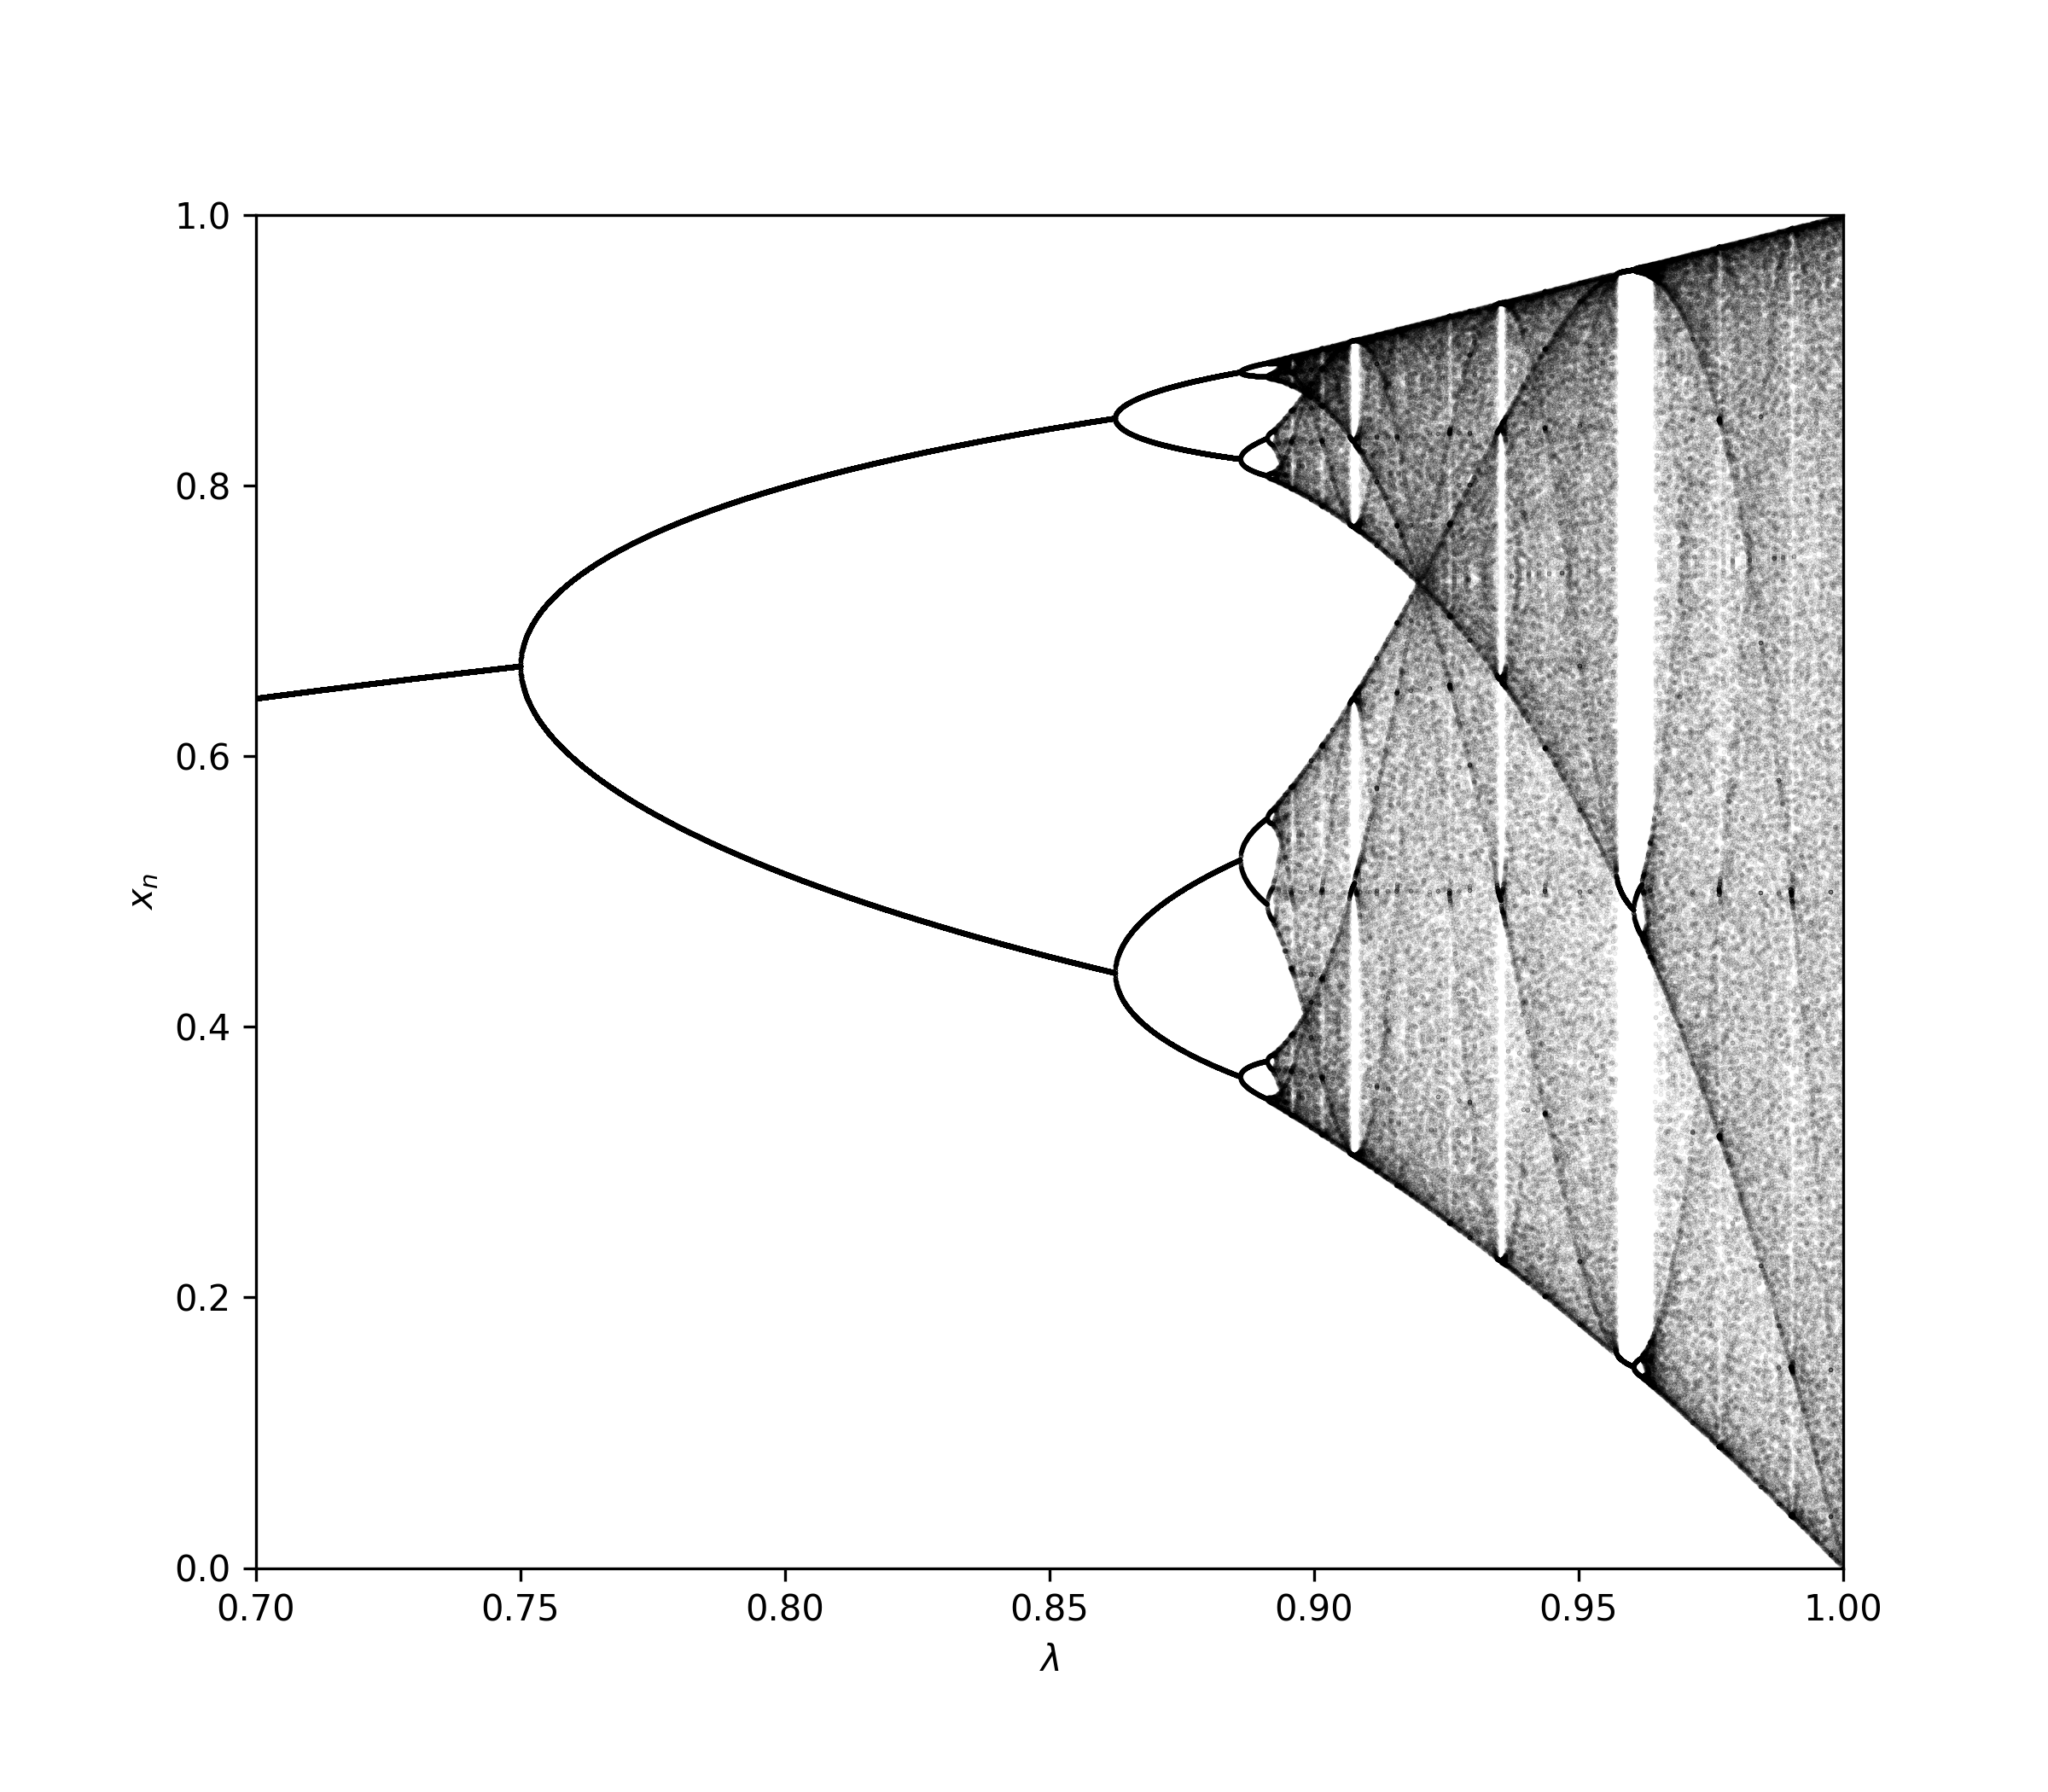
\includegraphics[width=0.5\textwidth]{figures/20_mappa_logistica_ Feigenbuam.png}
    \caption{\scriptsize Andamento degli ultimi 40 step su 20000 al variare di $\lambda$ (i valori che assume $x$ per una traiettoria sono linee verticali). Si nota come dopo qualche diramazione dei valori stabili subentra il caos nella mappa. \\
    La condizione iniziale per ogni traiettoria è $x_0=0.5$.}
    \label{fig:figures-20_mappa_logistica_-Feigenbuam-png}
\end{figure}
\noindent
Questo grafico raffigura gli ultimi valori assunti dalla mappa su un set di $n$ iterazioni. L'idea del grafico è che, dopo un certo tempo, le traiettorie termalizzino su dei punti stabili. Se questo non succede e la mappa si spalma in tutti i possibili valori del dominio allora significa che è subentrato il caos.\\
Si nota come anche per $\lambda > 3 /4$ possano esistere punti attrattori per la mappa. Infatti emergono nel caos delle piccole zone nel quale la mappa assume "pochi" valori. \\
Possiamo anche vedere qual'è l'andamento della media degli esponenti di Lyapunov per la mappa tangente al variare di $\lambda$ in figura \ref{fig:figures-20_mappa_logistica_lyapunov-png}.\\
Si nota subito come, appena prevale il caos nel sistema, gli esponenti siano mediamente positivi. 
\begin{figure}[H]
    \centering
    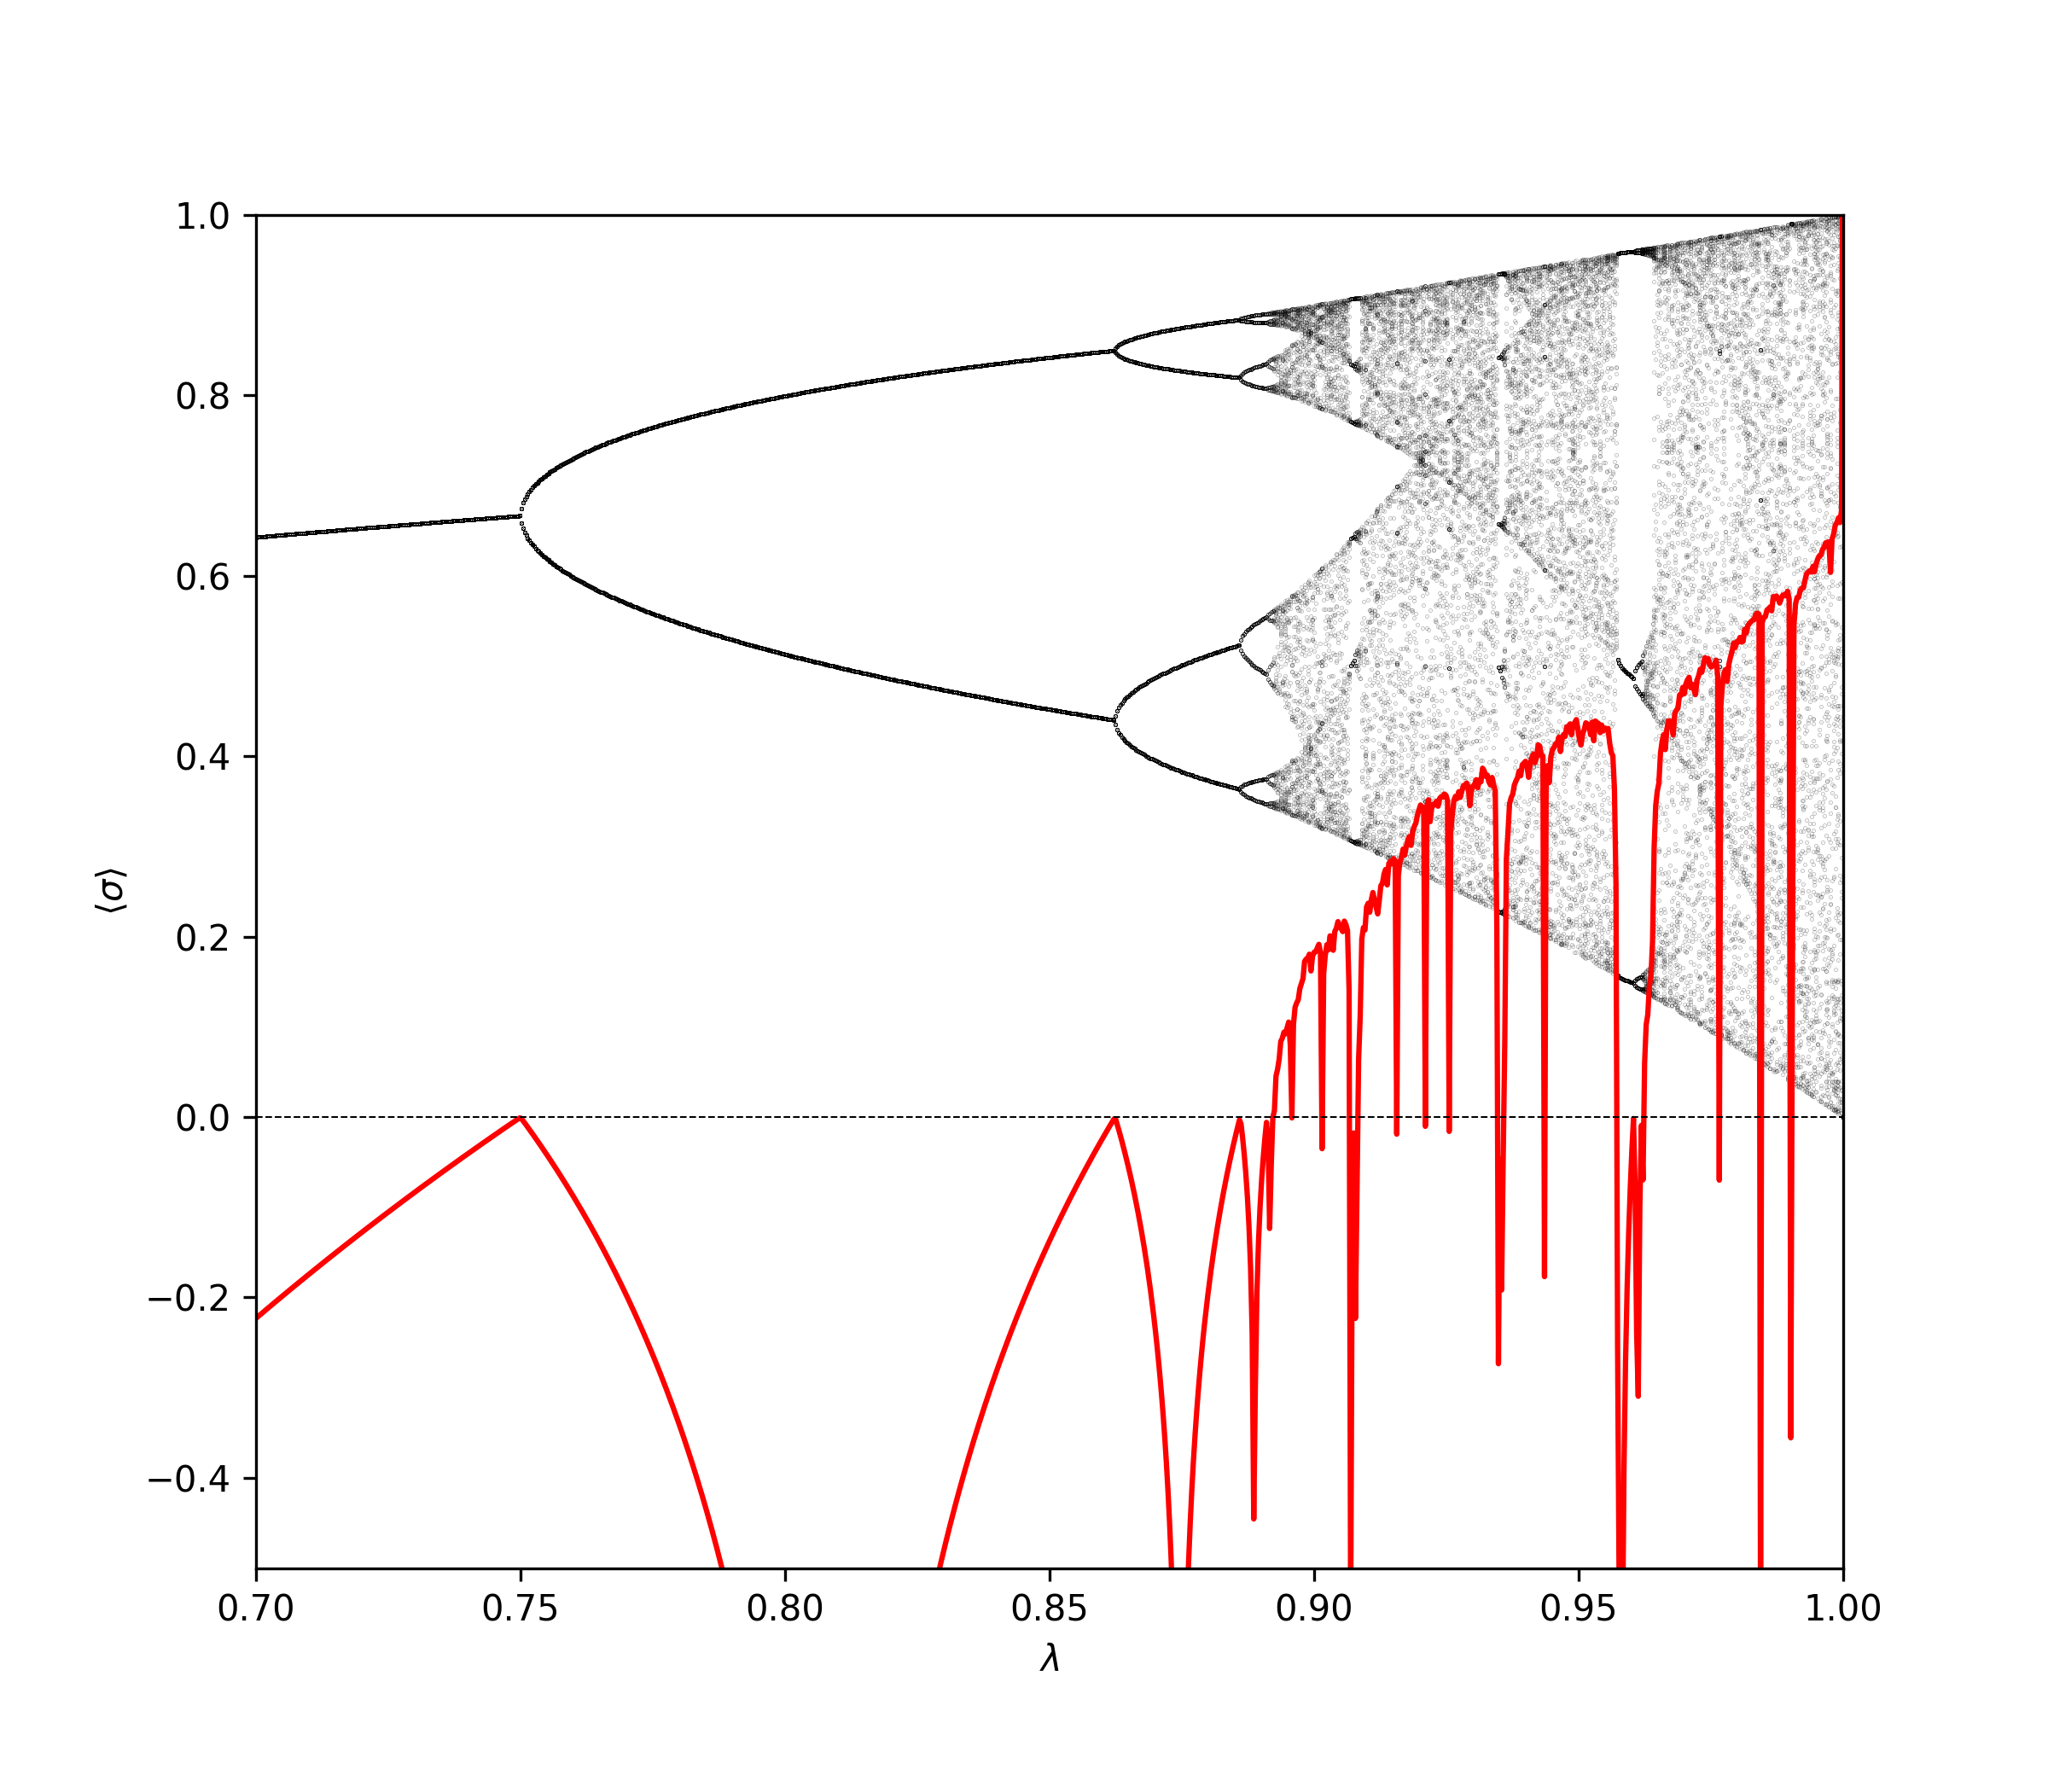
\includegraphics[width=0.5\textwidth]{figures/20_mappa_logistica_lyapunov.png}
    \caption{\scriptsize Andamento della media degli esponenti di Lyapunov al variare del parametro $\lambda$. }
    \label{fig:figures-20_mappa_logistica_lyapunov-png}
\end{figure}
\subsection{Calcolo degli esponenti di Lyapunov in pratica}%
\label{sub:Calcolo degli esponenti di Lyapunov in pratica}
Calcolare gli esponenti di Lyapunov è solitamente molto complicato. Quello che si fa nella maggior parte dei casi è valutare solo il più grande.\\
Infatti non serve valutare ogni esponente: se il più grande è maggiore di $0$ allora possiamo automaticamente dedurre di essere in presenza di un sistema caotico.
\subsubsection{Algoritmo di Benedettin et al. (1976)}%
\label{subsub:Algoritmo di Benedettin et al. (1976)}
La congettura di fondo era di capire da dove venisse fuori il fattore $\hbar $ nella meccanica quantistica. Si ipotizzò che tale valore fosse una soglia al caos: poteva essere che, in un sistema reale, esistesse un valore della azione sopra al quale emergesse il caos, si voleva capire se questo valore fosse parente di $\hbar $.\\
Si parte da una equazione del moto:
\[
    \dot{\vect{x}}=F(\vect{x})
.\] 
Se ne fa la dinamica tangente:
\[
    \frac{\text{d} }{\text{d} t} \delta\vect{x}_i = \sum_{J}^{} \frac{\partial F_i}{\partial X_J} \delta\vect{X}_J
.\] 
Immaginando che la variazione $\delta\vect{x}_i$ (iterata $i$-esima) vada esponenzialmente nel tempo:
\[
    \delta\vect{x}_i(t) \sim e^{\sigma t}\delta x_i(0)
.\] 
Possiamo pensare che questo $\sigma$ sia il valore più grande tra gli esponenti di Lyapunov.\\
Definiamo il modulo delle $\delta\vect{x}_i$:
\[
    d(t)=\sqrt{\sum_{i}^{} \left|\delta x_i(t)\right|^2} 
.\] 
Mi aspetto che anche questa quantità abbia un andamento asintotico con l'esponente di Lyapunov maggiore:
\[
    d(t)\sim e^{\sigma t}d(0)
.\] 
Possiamo allora valutare $\sigma$ nel seguente modo:
\[
    \sigma  = \lim_{\substack{t \to \infty \\ d(0)\to 0}} \frac{1}{t}\ln\left(\frac{d(t)}{d(0)}\right)
.\] 
L'algoritmo operativo prevede di partire con $d(0) = 1$, integrare la mappa con un passo grande $\tau$ e rinormalizzare per ogni step il valore $d(n\tau)$ con $d(0)$. \\
In conclusione si valuta la $\sigma$ come:
\[
    \sigma  = \frac{1}{N\tau}\sum_{J}^{} \ln\left(\frac{d_J}{d(0)}\right)=\frac{1}{N\tau}\sum_{J}^{} \ln\left(d_J\right)
.\] 
\subsubsection{Altri algoritmi per il calcolo di più esponenti di Lyapunov}%
\label{subsub:Altri algoritmi per il calcolo di più esponenti di Lyapunov}
Quando vogliamo calcolare più esponenti di Lyapunov si fa uso dell'algoritmo di Woolf et al.\\
Il problema di questo calcolo deriva dal fatto che, in un sistema Hamiltoniano abbiamo spesso combinazioni di autovalori positivi e negativi. \\
In questi in particolare le variabili sono coniugate è più problematico calcolare gli autovalori in modo preciso.\\
In conclusione siamo sempre in grado di valutare la somma degli autovalori, calcolare il loro valore preciso è molto più complicato.
\clearpage

\section{Identificare Il caos: Caos Globale}%
\label{sec:Lezione 20}
\mylocaltoc
\subsection{K.S. Entropy}%
\label{sub:K.S. Entropy}
Prendiamo un sistema dinamico come una mappa Hamiltoniana che conserva una certa misura su un insieme $X$.\\
Supponiamo di introdurre una partizione di $X$ chiamata $Q$ tale per cui non ci sono sovrapposizioni tra le partizioni $Q_i$.\\
Inoltre chiediamo una ipotesi più forte: un punto $x\in X$ che appartiene ad uno solo dei $Q_i$ e vi appartiene anche ogni sua $n$-esima iterata della mappa $T$.\\
Possiamo costruire una dinamica simbolica: una sequenza di interi $\left\{x_n\right\}$ tali che:
\[
    T^nx \in Q_{x_n}
.\] 
Si dice \textbf{partizione generatore} la partizione $Q$ se per ogni $x$ si ha una unica dinamica simbolica (quindi una unica sequenza di interi).
\subsubsection{Strumento per definire l'entropia: Baker Trasformation}%
\label{subsub:Applicazione: Baker Trasformation}
Prendiamo un sistema bidimensionale con variabili $p,q$, la trasformazione di Baker ha la seguente forma:
\[
    T(p,q)=
    \begin{cases}
	2p ,\  q /2 \qquad &\text{se } 0 \le p < 1 /2\\
	2p-1, \ q /2 + 1 /2 \qquad &\text{se } 1 /2 \le p \le 1
    \end{cases}
\]
\begin{figure}[H]
    \centering
    \incfig{21_baker}
    \caption{\scriptsize Passaggi operativi della mappa di Baker. Si fa come con il pane: si mette sopra e poi si schiaccia.}
    \label{fig:21_baker}
\end{figure}
\noindent
Con questa mappa è comodo scrivere le coordinate $p,q$ in base 2:
\[
    p = \sum_{k=0}^{-\infty} s_k 2^{k-1} \qquad q = \sum_{k=1}^{\infty} s_k 2^{-k}
.\] 
Le potenze $k$ dello sviluppo sono negative, questo perché le variabili vanno da $0$ a $1$. Le $s_k$ inoltre possono valere $0$ o $1$.\\
Ogni punto in questa base è esprimibile come sequenza di $0$ e $1$ nel seguente modo:
\begin{equation}
    x_i = \left(\ldots, s_{-2}, s_{-1}, s_0, s_1, \ldots\right)
    \label{eq:21_baker_list}
\end{equation}
Vediamo come agisce la mappa con un esempio pratico: se si ha $0<p< 1 /2$ e si applica $T$ avremmo che 
\[
    p\to 2p, \qquad q \to q /2
.\] 
Nel linguaggio della lista dei $s_i$ questo significa che tutti gli $s_i$ andranno verso destra. Quindi l'evoluzione della mappa è semplicemente lo spostare i coefficienti $s_i$ verso destra con la notazione \ref{eq:21_baker_list}.\\
Abbiamo anche un effetto di bordo tra le $p$ e le $q$: $s_0$ perchè dovrebbe andare in $s_1$ visto che il primo è un fattore di $p$ e l'altro è un fattore di $q$?\\
La risposta è proprio nella natura della trasformazione che "ruota" lo spazio $p$ e $q$. Facendo un controllo nel caso specifico patologico ($p=1/2$) si vede subito che il coefficiente $s_0$ deve necessariamente andare in $s_1$.\\
\subsubsection{Definizione di KS entropy}%
\label{subsub:Definizione di KS entropy}
Introduciamo adesso la partizione che deriva dalla intersezione delle iterate della trasformazione di Baker.
\begin{figure}[H]
    \centering
    \incfig{21_def_E}
    \caption{\scriptsize Mappa di Baker con intersezione delle partizioni.}
    \label{fig:21_def_E}
\end{figure}
\noindent
Potremmo iterare la procedura più volte ottenendo ogni volta una potenza di due in più nel numero di partizioni.\\
Si definisce  KS Entropy:
\[
h_{_{KS}} = \text{sup}\left( \lim_{n \to \infty} \frac{h\left[ AV(TA)V(T^2A)V\ldots VT^{n-1}A\right]}{n}\right)
.\] 
con 
\[
    h(A)=-\sum_{i}^{} p_i\ln (p_i)
.\] 
Dove $p_i$ è l'area della partizione $i$.\\
Nel caso della mappa di Baker si ha che il numero di partizioni generate alla $n$-esima iterazione (considerando anche l'operatore di intersezione $V$) è $2^{n}$. L'area di ogni partizione sarà allora $2^{-n}$ e l'entropia di KS vale:
\[
    h_{_{KS}} = \frac{1}{n}\sum_{i}^{2^{n}} \left(\frac{1}{2^{n}}\right)n\ln\left(\frac{1}{2}\right) = \ln 2
.\] 
Sempre nel caso della Baker trasform. proviamo a calcolare gli esponenti di Lyapunov: 
\[
    \begin{pmatrix} p \\ q \end{pmatrix}_{n+1} = 
    \begin{pmatrix} 
	2 & 0 \\
	0 & 1/2
    \end{pmatrix} 
    \begin{pmatrix} p \\ q \end{pmatrix}_n
.\] 
Si vede subito che gli autovalori in questione sono:
\[
    \lambda_1 = 2 \qquad \lambda_2 = 1 /2
.\] 
Quindi gli esponenti di Lyapunov per la mappa sono $\pm \ln 2$. Il più grande tra i due esponenti è proprio l'entropia di KS, è un caso?
\begin{redbox}{Teorema di Piesin}
    La KS entropy è la somma degli esponenti di Lyapunov positivi.
    \[
        h_{_{KS}} = \int_{P}^{} \sum_{\lambda_i >0}^{} \lambda_id\mu 
    .\] 
    In cui $\lambda_i$ sono gli esponenti di Lyapunov in una regione di energia $E$ di misura $d \mu$.
\end{redbox}
\noindent
\subsection{Indicatori di Caos globale}%
\label{sub:Indicatori di Caos globaliIndicatori di Caos globale: metodo di Chirinkov}
\subsubsection{Metodo di Chirinkov}%
\label{subsub:metodo di Chirinkov}
L'idea alla base per trovare il caos globale è quella di cercare, anziché le singole traiettorie caotiche, delle intere strutture caotiche nello spazio delle fasi.\\
Partiamo da un sistema Hamiltoniano integrabile perturbato:
\[
    H(I,\theta) = H_0(I) + \epsilon H_I(I, \theta)
.\] 
Scriviamo la perturbazione in componenti spettrali di Fourier:
\[
    H(I,\theta) = H_0(I) + \epsilon \sum_{m}^{} H_m(I)e^{im\theta}
.\] 
Sappiamo che la mappa per l'Hamiltoniana imperturbata è la seguente:
\[
    \begin{cases}
	I_i = I_i(0)\\
	\theta_i = \omega_i(I)t + \theta_i(0)
    \end{cases}
.\] 
Con la pulsazione $\omega$ che è definita da:
\[
    \omega_i = \frac{\partial H_0}{\partial I_i} 
.\] 
Inseriamo la perturbazione e ipotizziamo che questa abbia una sola componente spettrale:
\[
    H(I,\theta) = H_0(I) + \epsilon H_m(I)e^{im\theta}
.\] 
Allora abbiamo visto che:
\[\begin{aligned}
    &\dot{I}_i = -i \epsilon  m_i H_m(I)e^{im\theta}\\
    &\dot{\theta}_i = \omega_i(I) + \epsilon  H'_m(I)e^{im\theta}
.\end{aligned}\]
E all'ordine $\epsilon$  la soluzione è:
\[
    I_i = I_i(0)-\frac{\epsilon m_i H'_m(I_0)e^{i(m\cdot \omega)t + i\delta}}{m\cdot \omega}
.\] 
La trasformazione canonica "astuta" che permette di rendere integrabile l'Hamiltoniana al primo ordine in $\epsilon$ in questo caso è:
\[
    F = m_{\perp}I
.\] 
Dove $m_{\perp}$ è tale per cui $m_{\perp}\cdot m = 0$. In tal caso la trasformazione canonica elimina la risonanza.\\
Questo metodo funziona quando abbiamo una sola risonanza, con più risonanze non è possibile "curare" il sistema: la teoria perturbativa non risolve in tutto lo spazio con più risonanze.\\
Visivamente il caos arriva quando si hanno sistemi nello spazio delle fasi del tipo:
\begin{figure}[H]
    \centering
    \incfig{21_risonanze}
    \caption{\scriptsize Spazio delle fasi in presenza di due risonanze: quando i lobi si avvicinano iniziano a rompersi i tori e a quel punto siamo in presenza di un caos globale.}
    \label{fig:21_risonanze}
\end{figure}
\begin{exmp}[Mappa standard]
    Nel caso della mappa standard si ha:
    \[\begin{aligned}
	H(I, \theta, t) =& \frac{I^2}{2} + 2\pi k \cos\theta  \sum_{m = -\infty}^{\infty} \delta (2\pi m-t) = \\
	=& \frac{I^2}{2} + k \sum_{n= -\infty}^{\infty} \cos (\theta-nt)
    .\end{aligned}\]
    La mappa che abbiamo visto nelle lezioni precedenti è proprio questa integrata su un periodo.\\
    Vediamo che in questo caso generale escono fuori dei termini del tipo:
    \[
	H^{(n)}=\frac{I^2}{2}+k \cos\psi_n \qquad \psi_n = \theta-nt
    .\] 
    Abbiamo un set di Hamiltoniane risonanti con 
    \[
        \omega_n \equiv n
    .\] 
    Possiamo trovare la larghezza dell'"occhio" $\Delta\omega$ valutando la $I$ nel minimo del potenziale periodico:
    \[
        0 = \frac{I^2}{2}-k \implies  \Delta\omega_n \equiv I_{\text{max}, n} = 2\sqrt{k} 
    .\] 
    Come abbiamo detto in precedenza le $\omega$ sono numeri interi $n$, quindi tra una risonanza e l'altra c'è una distanza unitaria.\\
    Per questo motivo possiamo affermare che i lobi iniziano a toccarsi quando la loro distanza vale $1$, se due lobi distano tale valore significa che la larghezza del singolo occhio vale $1 /2$:
    \[
        \frac{1}{2} = 2k^{1 /2} \implies  k = \frac{1}{16}
    .\] 
    Per tale valore di $k$ (e per valori minori) nel sistema si ha una forma di caos globale. Possiamo verificare la cosa andando a setacciare la mappa standard al variare di $k$:
    \begin{figure}[H]
        \centering
	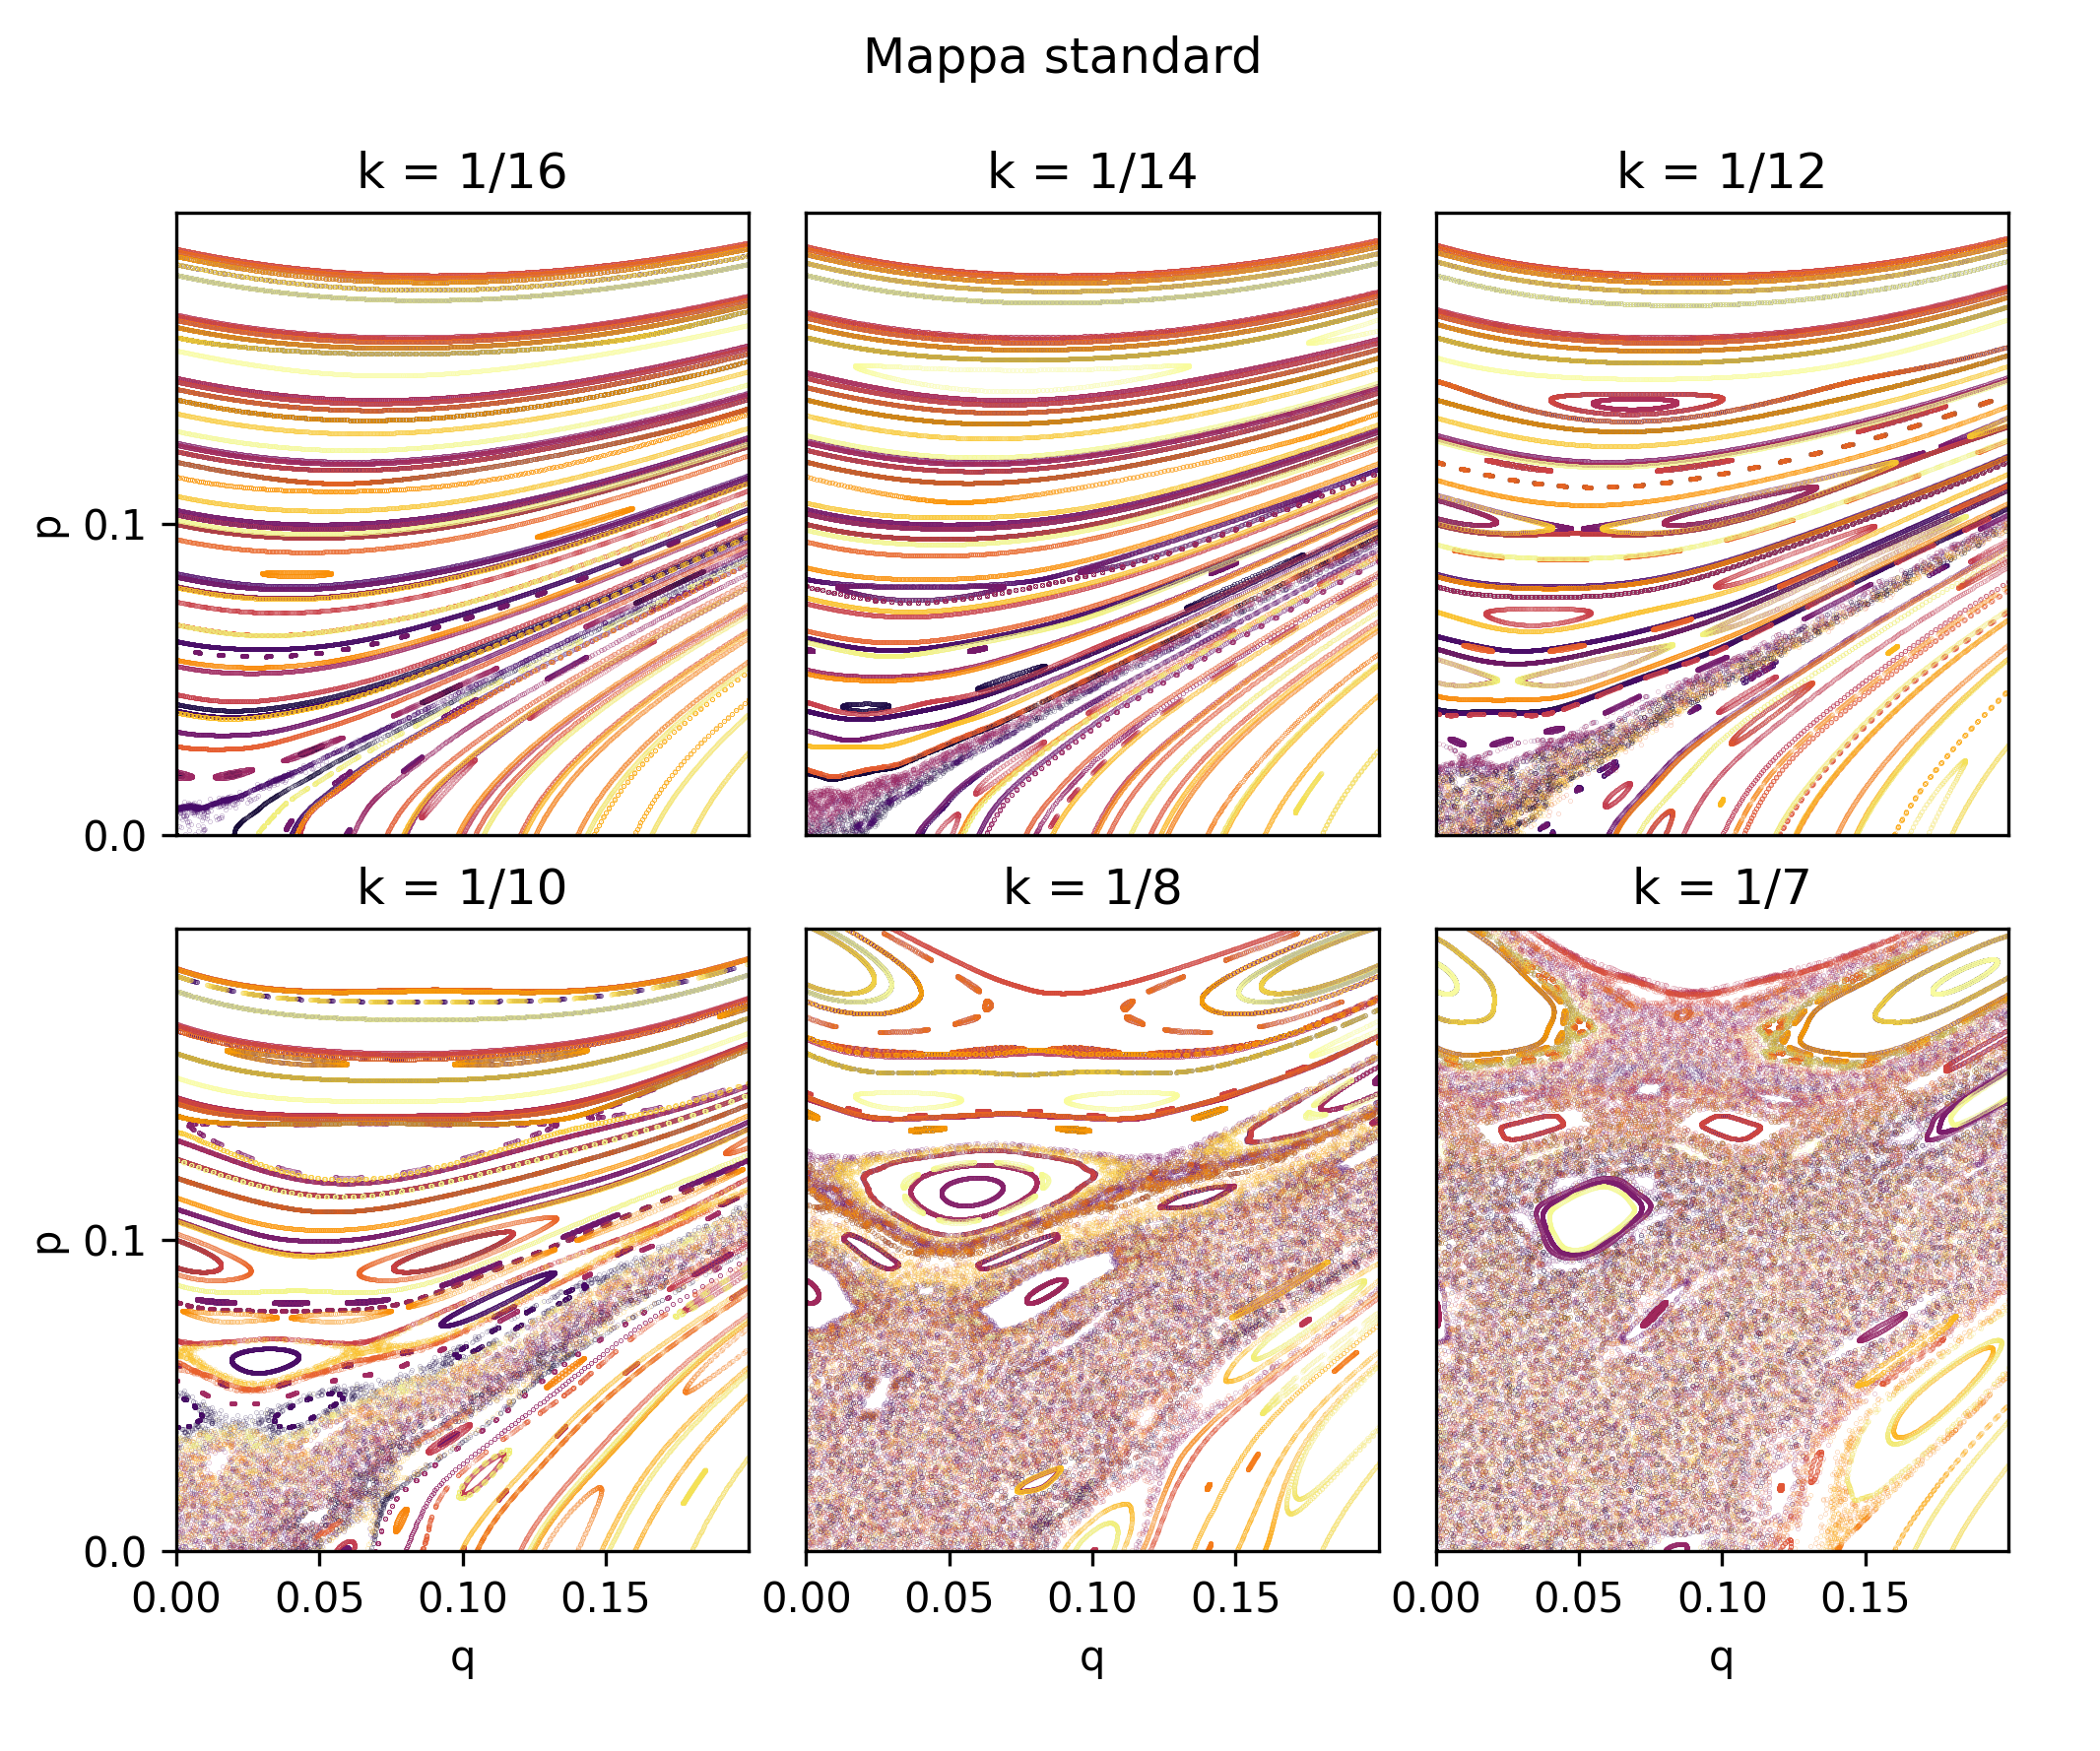
\includegraphics[width=0.47\textwidth]{figures/21_standard_maps.png}
        \caption{\scriptsize Zoom della mappa standard: si usano gli stessi parametri iniziali per tutte le traiettorie e si fa variare $k$ nella mappa.\\
	i primi cenni di caos in basso a sinistra (in tutte le figure) si hanno per $k = 1 / 16$.}
        \label{fig:figures-21_standard_maps-png}
    \end{figure}
\end{exmp}
\noindent
\begin{exmp}[Sistema di Henon-Hieles]
    Questo esempio è un ripasso della teoria perturbativa ed una applicazione al criterio di Chirinkov.\\
    Prendiamo la seguente Hamiltoninana con perturbazione:
    \[
        H = \frac{q_x^2+q_y^2}{2} + \frac{p_x^2+p_y^2}{2} + \epsilon q_x^2q_y^2
    .\] 
    La trasformazione canonica per le variabili azione angolo ci conduce a:
    \[
        H_0 = \omega_xI_x + \omega_yI_y
    .\] 
    Riscriviamo anche la trasformazione canonica inversa per completezza, come sempre:
    \[
        \begin{cases}
            q_x =\sqrt{2I_x} \cos\theta_x\\
	    q_y = \sqrt{2I_y} \cos\theta_y
        \end{cases}
    .\] 
    Il termine di perturbazione in questa base si presenta come:
    \[
        H_I = \epsilon 4 I_xI_y\cos^2\theta_x\cos^2\theta_y
    .\]  
    Facendo la teoria perturbativa dobbiamo trovare una trasformazione $S$ tale che la nuova Hamiltoniana del sistema sia del tipo:
    \[
	K(\vect{J}) = K_0(\vect{J}) + \epsilon K_1(\vect{J})
    .\] 
    Quindi cerchiamo di rimuovere la dipendenza dalle variabili angolo.
    \[
	S = S_0 + \epsilon S_1 = J_x\theta_x + J_y\theta_y + \epsilon S_1(\vect{J}, \vect{\theta})
    .\] 
    Quindi le nuove variabili sono legate alle vecchie dalle relazioni che conosciamo:
    \[\begin{aligned}
	& I_x = J_x +\epsilon  \partial_{\theta_x}S_1;  &\quad I_y = J_y +\epsilon  \partial_{\theta_y}S_1\\
	& \varphi_x = \theta_x +\epsilon  \partial_{J_x}S_1 &\quad \varphi_y = \theta_y + \epsilon\partial_{J_y}S_1
    .\end{aligned}\]
    Ripetendo ancora si ha che:
    \[
	H_0(\partial_{\theta_x}S, \partial_{\theta_y}S) + \epsilon  H_I(\partial_{\theta_x}S, \partial_{\theta_y}S, \vect{\theta}) = 
	K_0(\vect{J})+\epsilon K_1(\vect{J})
    .\] 
    Quindi l'Hamiltoninana all'ordine 0 è:
    \[
	K_0(J) = \omega_xI_x + \omega_yI_y
    .\] 
    Quella all'ordine $\epsilon$ invece:
    \[\begin{aligned}
	K_1(J) =& \omega_x\partial_{\theta_x}S_1 + \omega_y\partial_{\theta_y}S_1 + \\
	       &+ \epsilon 4 J_xJ_y\cos^2\theta_x\cos^2\theta_y
    .\end{aligned}\]
    Come abbiamo fatto in una dimensione si ha che $K_1$ non deve dipendere dagli angoli $\vect{\theta}$, quindi possiamo integrarlo:
    \[\begin{aligned}
	K_1(\vect{J}) &= \frac{1}{4\pi^2}\int_{0}^{2\pi} \int_{0}^{2\pi} d\theta_xd\theta_y \cos^2\theta_x\cos^2\theta_y 4J_xJ_y =\\
		      &=J_xJ_y
    .\end{aligned}\]
    In cui le derivate di $S$ sono andate via poiché periodiche (si annullano integrate sul periodo).\\
    Reinserendo $K_1$ nella equazione della Hamiltoniana al primo ordine non integrata si ottiene una equazione differenziale per la trasformazione $S_1$:
    \[
        \omega_x \partial_{\theta_x}S_1 + \omega_y \partial_{\theta_y}S_1 = J_xJ_y\left(1-4\cos^2\theta_x\cos^2\theta_y\right)
    .\] 
    Facendo uso di formule trigonometriche possiamo far sparire i termini non lineari nei coseni:
    \[\begin{aligned}
	\omega_x& \partial_{\theta_x}S_1 + \omega_y \partial_{\theta_y}S_1 =\\
	=&  -J_xJ_y\left[\cos (2\theta_x)+\cos(2\theta_y) + \right.\\
	 &+ \left.  \cos (2(\theta_x-\theta_y)) + \cos (2(\theta_x+\theta_y))\right]
    .\end{aligned}\]
    Questa equazione può essere integrata analiticamente e porta al seguente risultato:
    \[\begin{aligned}
	S_1 =& -J_xJ_y \left(\frac{\sin (2\theta_x)}{2\omega_x} + \frac{\sin(2\theta_y)}{2\omega_y} + \right.\\
	     & + \left. \frac{\sin (2(\theta_x-\theta_y))}{\omega_x-\omega_y} + \frac{\sin (2(\theta_x+\theta_y))}{\omega_x+\omega_y}\right)
    .\end{aligned}\]
    Notiamo come non sia possibile fare uno sviluppo perturbativo che rimuova tutte le risonanze.
\end{exmp}
\noindent
\subsubsection{Criterio di Melnikov}%
\label{sub:Criterio di Melnikov}
Supponiamo di avere un punto iperbolico e poniamoci in un sistema con una Hamiltoniana integrabile imperturbata. Supponiamo che tale punto fisso presenti un'orbita omoclinica $\phi (t)$ stabile:
\begin{figure}[H]
    \centering
    \incfig{21_omoclinica}
    \caption{\scriptsize Orbita omoclinica stabile per il sistema. Notiamo che per questo tipo di orbita non c'è formazione di caos: i manyfold non si incrociano, rientrano nel punto critico in modo continuo.}
    \label{fig:21_omoclinica}
\end{figure}
\noindent
Inseriamo adesso la perturbazione nel sistema, dal punto di vista di Melnikov quello che succede è che si modificano i manyfold nel seguente modo:
\begin{figure}[H]
    \centering
    \incfig{21_melni_pertrutbato}
    \caption{\scriptsize Orbite perturbate rispetto alla omoclinica.}
    \label{fig:21_melni_pertrutbato}
\end{figure}
\noindent
Sappiamo che se $\vect{x}_n$ (il manifold instabile) ed $\vect{x}_s$ (il manifold stabile) si incrociano una volta allora si genera il caos. Il criterio di Melnikov si basa proprio sul capire quanto sono distanti i manyfold e valutare la possibilità che si incrocino. \\
Definiamo quindi la distanza tra i due manyfold (in ogni punto appartenente ai due manyfold) come $\vect{\Delta} (t)$. 
\[
    \vect{\Delta} (t) = \vect{x}_n - \vect{x}_s
.\] 
Se dimostriamo che questa quantità va a zero in un punto dello spazio delle fasi allora sappiamo che nel sistema emerge del caos globale.\\
Un primo metodo è quello di valutare $\left|\vect{\Delta} (t)\right|$ e trovarne il minimo, se il minimo si annulla allora concludiamo.\\
Una cosa più semplice è calcolare la quantità:
\[
    d = \vect{\Delta}\cdot \hat{n}
.\] 
Dove $\hat{n}$ è la normale alla separatrice imperturbata $\phi (t)$. \\
Per calcolare $d$ partiamo dalle equazioni del moto per la separatrice imperturbata:
\[
    \begin{pmatrix} \dot{q} \\ \dot{p}\end{pmatrix}_{0}  = 
    \begin{pmatrix}  
	f_q \\ f_p
    \end{pmatrix}_{0}
.\] 
Per trovare $\hat{n}$ possiamo fare il prodotto vettoriale tra la terza coordinata $\hat{z}$ e la velocità della traiettoria imperturbata $\phi (t) (\equiv \vect{x}_0)$.
\[
    \hat{n} = \hat{z} \wedge \dot{\vect{x}}_0
.\] 
La quantità $d$ può essere trovata sfruttando la ciclicità del prodotto:
\begin{equation}
    d(t) = \left| \dot{\vect{x} }_0 \wedge \vect{\Delta}\right| = f_q\Delta_p - f_p \Delta_q
    \label{21:eq_delta}
\end{equation}
Adesso cerchiamo una equazione differenziale per la $\Delta$, facendo la derivata esplicita della \ref{21:eq_delta}:
\begin{equation}
\begin{aligned}
    \dot{d} = & (\partial_{q}f_q \dot{q}_0 + \partial_{p}f_p \dot{p}_0)\Delta_p +\\
	      & - (\partial_{q}f_q \dot{q}_0 + \partial_{p}f_p \dot{p}_0)\Delta_q +\\
	      & + f_q \dot{\Delta}_p - f_p \dot{\Delta}_q
	      \label{21:eq_dotd}
.\end{aligned}
\end{equation}
Proviamo a semplificare questa espressione, partiamo dalla definizione della quantità vettoriale $\vect{\Delta}$:
\[
    \vect{\Delta}  = \vect{x}_n - \vect{x}_0 - (\vect{x}_s-\vect{x}_0)
.\] 
Anziché valutare l'intero tratto $\vect{\Delta}$ concentriamoci solo sul calcolo del primo termine: $\vect{x}_n-\vect{x}_0$. Questo calcolo è più semplice, operativamente l'altro termine può esser sempre calcolato con il metodo sotto.
\[
    \begin{pmatrix} \dot{q}_n \\ \dot{p}_n \end{pmatrix} =
    \left.\begin{pmatrix} f_q \\ f_p \end{pmatrix}\right|_{n} + \epsilon  \left.\begin{pmatrix} g_q \\ g_p \end{pmatrix}\right|_{n}  
.\] 
Questa è l'equazione dell'evoluzione della traiettoria con l'aggiunta del pezzo di perturbazione.\\
Possiamo sviluppare al primo ordine la $f_q$ vicino all'orbita omoclinica (visto che la stiamo valutando sull'orbita perturbata $n$):
\[
    f_q(\vect{x}_0 + \vect{x}_n - \vect{x}_0) \simeq f_q(\vect{x}_0) + \nabla \left.f_q\right|_{q_0}(\vect{x}_n-\vect{x}_0)
.\] 
Prenderemo poi l'ordine più basso in $\epsilon$ della perturbazione.\\
Reinserendo nella equazione sopra questo sviluppo si ha:
\[\begin{aligned}
    &\begin{pmatrix} d /dt(q_n - q_0) \\ d /dt(p_n - p_0) \end{pmatrix} = \\
    &\qquad = \begin{pmatrix} 
	\partial_{q}f_q(q_n-q_0) + \partial_{p}f_q(p_n-p_0)\\
	\partial_{q}f_p(p_n-p_0) + \partial_{p}f_p(q_n-q_0)
    \end{pmatrix} + \epsilon \begin{pmatrix} g_q \\ q_p \end{pmatrix}_{0}
.\end{aligned}\]
Quindi abbiamo le equazioni differenziali per $\dot{\vect{\Delta}}$:
\[
    \begin{cases}
        \dot{\Delta}_q = \partial_{q}f_q\Delta_q + \partial_{p}f_q\Delta_p + \epsilon g_q\\
	\dot{\Delta}_p = \partial_{q}f_p \Delta_q + \partial_{p}f_p\Delta_p + \epsilon g_p
    \end{cases}
\] 
Si tratta adesso di reinserire queste equazioni nella \ref{21:eq_dotd} e svolgere un po d'algebra.\\
Inserendo la notazione per il prodotto esterno tra  $f$ e $g$:
\[
    f \wedge g = f_qg_p - f_p g_q
.\] 
Possiamo scrivere il risultato cercato: la ODE per $\dot{d}$
\[
    \dot{d} = (\partial_{q}f_q + \partial_{p}f_p)d + \epsilon f \wedge g
.\] 
Risolvendo si ha che:
\[
    d(t) = \int_{-\infty}^{t} dt \exp\left(\int\partial_{q}f_q \partial_{p}f_p ds\right) f \wedge g
.\] 
Se questo oggetto ha degli zeri allora nel sistema è presente il caos globale.\\
Nel caso di un sistema Hamiltoniano si ha che:
\[
    \partial_{q}f_q = \partial_{q}\partial_{p}H = \partial_{p}\partial_{q}H = - \partial_{p}f_p
.\]
Quindi l'esponenziale nell'integrale si cancella.\\
Facendo lo stesso ragionamento con $\vect{x}_s$ si ottiene che l'intero tratto vale:
\[
    d(t) = \int_{-\infty}^{\infty} dt \exp\left(\int\partial_{q}f_q \partial_{p}f_p ds\right) f \wedge g
.\] 
\begin{exmp}[Pendolo perturbato]
    Prendiamo la mappa Hamiltoninana:
    \[
        \begin{pmatrix} \dot{\varphi} \\ \dot{y}\end{pmatrix} =
	\begin{pmatrix} y \\ -\sin\varphi \end{pmatrix} +
	\epsilon  \begin{pmatrix} 0 \\ a - \alpha y + A \sin (\Omega  t)\end{pmatrix} 
    .\] 
    La $\varphi_0$ in questo caso la si sa calcolare, il risultato è il seguente:
    \[\begin{aligned}
	&\varphi_0(t) = \pm 2 \arctan(\sinh(t))\\
	& y_0(t) = \pm 2 \text{sech}(t)
    .\end{aligned}\]
    In questo caso il prodotto esterno $f \wedge g$ vale:
    \[
	f \wedge g = y (a-\alpha y + A \sin (\Omega  t))
    .\] 
    Il sistema è Hamiltoniano poiché:
    \[
        \partial_{q}f_p + \partial_{p}f_p = 0
    .\] 
    Quindi possiamo calcolare direttamente la quantità $d(t)$, che definiamo qua come $M(t)$:
    \[
	M(t_0)= \int_{-\infty}^{\infty} y_{n} (t-t_0)\left[a+A\sin (\Omega  t) - \alpha y_n (t-t_0)\right]dt
    .\] 
    In cui si valuta la $y_n$ con una fase $t-t_0$ rispetto al $\sin (\Omega t)$.
    Questo integrale si risolve con il risultato:
    \[
	M(t_0)= \pm 2\pi a - 8\alpha  \pm 2\pi\text{sech}\left(\frac{\pi\Omega}{2}\right)\sin (\Omega t)
    .\]
    I segni $\pm$  si riferiscono al fatto che possiamo trovarci nel "ramo" di sopra o di sotto rispetto allo zero delle $y$  nello spazio delle fasi.\\
    In conclusione possiamo studiare i punti di annullamento di $M$ al variare di $t_0$ per scoprire che il caos entra nel sistema appena vale la seguente disuguaglianza (si fissano $a$ e $\alpha$):
    \[
	A \ge \left|\pm a + \frac{4\alpha}{\pi}\right|\cosh(\frac{\pi\Omega}{2})
    .\] 
    Per valori di $A$ maggiori i manifold si incrociano nello spazio delle fasi dando il via al caos nelle modalità espresse dal teorema di Poincare. 
\end{exmp}
\noindent
Possono esistere fenomeni caotici che non sono "visti" dal criterio di Melnikov perché implicano delle strutture ancora più complicate nello spazio delle fasi.
\subsection{Calcolo degli esponenti di Lyapunov in processi di Wiener.}%
\label{sub:Calcolo degli esponenti di Lyapunov in processi di Wiener.}
Prendiamo un caso unidimensionale:
\[
    dx = -V' dt + dw
.\] 
Sappiamo che la distribuzione stazionaria per il processo ha la forma:
\[
    P_{\text{st}}(x) \sim \exp (-V(x))
.\] 
Per calcolare l'esponente di Lyapunov dobbiamo guardare uno scostamento infinitesimo dalla traiettoria $x_t$:
\[
    x_t + \delta x_t
.\] 
Inserendo nella equazione stocastica:
\[
    d(x_t + \delta x_t) = - V'(x_t + \delta x_t)dt + dw
.\] 
Svolgendo ed esplicitando i termini:
\[
    dx_t + d\delta x_t = -V'(x_t)dt - V''(x_t)dt\delta x_t + dw
.\] 
Definendo la variabile infinitesima:
\[
    \epsilon_t = \delta x_t
.\] 
Abbiamo una equazione differenziale del tipo:
\[
    d\epsilon_t = - V''(x_t)\epsilon dt
.\] 
Questa equazione differenziale ci dice che:
\[
    \epsilon_{t+\Delta t} = \exp\left(-V''(x_t) \Delta t\right)\epsilon_t
.\] 
Con $\Delta t$ "piccolo".\\
Possiamo allora calcolare l'esponente di Lyapunov con la definizione:
\[
    \lambda_t \sim \frac{1}{\Delta t}\ln\left(\frac{\epsilon_{t+\Delta t}}{\epsilon_t}\right) \sim -V''(x_t)
.\] 
Ovviamente per valutare la caoticità del sistema dobbiamo mediare sulle posizioni della traiettoria:
\[
    \lambda  = \left< \lambda_t\right> = - \left<V''\right>
.\] 
Possiamo esplicitare quest'ultimo conto:
\[\begin{aligned}
    -\left<V''\right> =& - \int V''e^{-V}dx =\\ 
		       & = - \int\left(\frac{\text{d} }{\text{d} x} V'e^{-V}+V'^2e^{-V}\right)dx = \\
		       & = 0 - \int  V'^2e^{-V}dx <0
.\end{aligned}\]
Quindi visto che $\lambda < 0 $ il sistema non è mai caotico. \\
Il problema diventa meno banale quando siamo di fronte ad un esperimento: vorremmo essere in grado di trovare gli esponenti di Lyapunov in un caso reale in cui non si hanno le equazioni differenziali stocastiche.
\subsection{Tecnica di Embedding per calcolare gli esponenti di Lyapunov in sistema reale.}%
\label{sub:Tecnica di Embedding per calcolare gli esponenti di Lyapunov in sistema reale.}
Prendiamo un segnale all'apparenza stocastico, ad esempio il seguente:
\begin{figure}[H]
    \centering
    \incfig{21_caos_signal}
    \caption{\scriptsize Segnale ignoto, vogliamo scoprire se presenta caos.}
    \label{fig:21_caos_signal}
\end{figure}
\noindent
Si procede facendo una operazione "inversa" rispetto alla mappa di Poincare: proiettiamo il sistema unidimensionale (in $x$) in un sistema $n$ dimensionale. \\
Dobbiamo quindi pensare che il segnale che si osserva sia solo una proiezione di un fenomeno a dimensionalità più elevata.\\
Per far questo si procede nel seguente modo:
\begin{itemize}
    \item Si definisce un tempo $\tau$ e si decide la dimensionalità $n$ che si vuole teorizzare.
    \item Si seleziona un punto sul tracciato: $x_0$ e si prendono gli $n-1$ punti che distano $\tau$ da $x_0$. Se ad esempio si selezionano 3 dimensioni si avrà $\vect{x}_0 = (x_0, y_0, z_0)$.
    \item Si itera la procedura con un altro punto $x_1$\ldots Si genera una sequenza di vettori $n$ dimensionali che identificano la traiettoria del sistema ad alta dimensionalità (arbitraria).
\end{itemize}
Il procedimento è illustrato in figura \ref{fig:21_embed}.
\begin{figure}[H]
    \centering
    \incfig{21_embed}
    \caption{\scriptsize Zoom del grafico precedente con procedura di Embedding.}
    \label{fig:21_embed}
\end{figure}
\noindent
Quindi avremo degli oggetti in generale del tipo:
\[
    \vect{x} (t)= \left\{x(t), x(t+\tau), x(t+2\tau), \ldots, x(t+(n-1)\tau) \right\}
.\] 
Vista la arbitrarietà del metodo sono state pensate una serie di tecniche entropiche per valutare la dimensionalità e $\tau$ come iper-parametri del sistema.\\
Per concludere gli esponenti di Lyapunov vengono fuori valutando la distanza tra le varie traiettorie $\vect{x} (t_i)$ più vicine. Se prendiamo ad esempio la distanza euclidea tra la traiettoria $\vect{x}_{n+1}$ e quella $\vect{x}_n$ (che chiamiamo $d$) abbiamo che:
\[
    \delta\vect{x}_{n+1} = d \delta\vect{x}_n
.\] 
Quindi per definizione di esponente di Lyapunov $\sigma$:
\[
    e^{N\sigma} = d
.\] 
Dove $N$ è il numero totale di punti.\\
Quindi se da questa analisi emergono dei $\lambda$ positivi possiamo affermare con certezza che il sistema è caotico, notiamo che invece non vale il viceversa: se si ottiene un esponente negativo potremmo essere semplicemente stati sfigati a beccare una regione nello spazio delle fasi priva di caos.
\subsection{Mixing delle traiettorie}%
\label{sub:Mixing delle traiettorie}
Se abbiamo delle divergenze esponenziali nelle traiettorie dello spazio delle fasi allora possiamo dedurre che il sistema realizzi un mixing.\\
Si parla di mixing quando la misura di due traiettorie distinte ha la proprieta:
\[
    \left<A(t)B(t)\right> \to  \left<A\right>\left<B\right> \qquad \text{con } t\to \infty
.\] 
Vediamo cosa significa in pratica a partire da un famoso esempio:
\begin{exmp}[Gatto di Arnold]
    Il sistema del gatto di Arnold è descritto dalla seguente mappa:
    \[
        T: \quad
	\begin{pmatrix} x_{n+1} \\ y_{n+1} \end{pmatrix}  = 
	\begin{pmatrix} 
	    1 & 1 \\
	    1 & 2
	\end{pmatrix} 
	\begin{pmatrix} x_n \\ y_n \end{pmatrix} 
	\quad \text{mod}x = \text{mod}y = 1
    .\]
    La mappa è Hamiltoniana poiché ha determinante unitario. \\
    Per capire come questo sistema realizza il mixing andiamo a studiare i punti fissi. Sappiamo che un punto fisso deve finire in se stesso dalla applicazione della mappa:
    \[
        \begin{cases}
            x = x+y -n \\
	    y = x + 2y - m
        \end{cases}
    .\] 
    In cui $n \in \left[0,1\right]$, $m \in \left[0,2\right]$ per via del modulo unitario.\\
    In particolare si ha $n=1$ solo se la $x$ esce dal quadrato unitario, lo stesso vale per la $y$ che potrebbe aver bisogno anche di una spinta di $-2$ per rientrare.\\
    Risolvendo per i punti fissi otteniamo i seguenti valori:
    \[
        y = n \qquad x = - y + m
    .\] 
    Quindi i punti fissi sono i quattro vertici del quadrato che, in sostanza, sono tutti lo stesso punto per via del modulo unitario.\\
    La mappa tangente invece è equivalente alla mappa stessa (si ottiene con le derivate miste):
    \[
        \begin{pmatrix} 
	    1 & 1 \\
	    1 & 2
	\end{pmatrix} 
    .\] 
    Gli autovalori e gli autovettori di questa mappa sono:
    \[
        \lambda_{\pm}= \frac{3 \pm \sqrt{5} }{2} \qquad
	\xi_{\pm} = \begin{pmatrix} 1 \\ \frac{1 \pm \sqrt{5} }{2} \end{pmatrix} 
    .\] 
    Notiamo che essendo la mappa Hamiltoniana i due autovalori devono essere uno l'inverso dell'altro, questa proprietà è rispettata dai $\lambda_{\pm}$.\\
    Possiamo quindi vedere come sono fatte le varietà stabili/instabili attorno ai quattro punti fissi. \\
    Scostandosi da ogni punto fisso di una quantità $\epsilon$ (per ciascuna delle due coordinate) e inserendo il punto "scostato" nella mappa si ottengono i seguenti risultati:
    \[\begin{aligned}
	&(\epsilon,\epsilon)\to (2\epsilon, 3\epsilon)\\
	& (1-\epsilon, \epsilon) \to (1, 1+\epsilon) \to (1, \epsilon)
    .\end{aligned}\]
    Quindi il primo punto è instabile, il secondo è stabile (non sappiamo se ci siamo posti esattamente sul manifold uscente/entrante, sappiamo solo che nei pressi degli scostamenti valutati c'è uno di questi due).\\
    I risultati per gli altri punti sono riportati in figura \ref{fig:21_stab_instab}.
    \begin{figure}[H]
        \centering
        \incfig{21_stab_instab}
	\caption{\scriptsize Stabilità dei punti fissi nel sistema di Arnold.}
        \label{fig:21_stab_instab}
    \end{figure}
    \noindent 
    Visto che abbiamo valutato gli autovalori della mappa tangente possiamo prendere il maggiore e valutarvi l'esponente di Lyapunov:
    \[
	\sigma  = \ln (\lambda_+) = \ln\left(\frac{3 + \sqrt{5} }{2}\right) > 0 
    .\] 
    Il sistema presenta caos.
    Possiamo vedere cosa succede alla mappa iterata due volte, facciamo il prodotto tra le matrici:
    \[
        \begin{pmatrix} 
	    1 & 1 \\
	    1 & 2
	\end{pmatrix} 
        \begin{pmatrix} 
	    1 & 1 \\
	    1 & 2
	\end{pmatrix} 
	= 
	\begin{pmatrix} 
	    2 & 3\\
	    3 & 5
	\end{pmatrix} 
	\qquad \text{mod}1
    .\] 
    Possiamo cercare nuovamente i punti fissi, procedendo nello stesso modo visto nel caso della mappa iterata una sola volta si arriva a ($x, y$):
    \[
        \left(\frac{1}{5}, \frac{3}{5}\right); \ \left(\frac{2}{5}, \frac{1}{5}\right); \ 
	\left(\frac{3}{5}, \frac{4}{5}\right); \ \left(\frac{4}{5}, \frac{2}{5}\right)
    .\] 
    E tutti questi sono ancora punti iperbolici i cui manifold si incrociano formando di nuovo caos. Gli autovalori della mappa tangente questa volta sono:
    \[
        \lambda_{\pm} = \frac{7 \pm \sqrt{45}}{2}
    .\] 
    Quindi abbiamo una mappa che induce una dinamica molto complicata e caotica già dalle prime iterazioni.
\end{exmp}
\noindent
\begin{exmp}[Trasformazione di Baker]
    Riprendiamo la trasformazione di Baker già vista nella precedente lezione:
    \[\begin{aligned}
	&
        \begin{cases}
            x_{n+1} = 2 x_n\\
	    y_{n+1} = y_n /2
	\end{cases} & \quad \text{se } 0 \le x_n \le  1 /2\\
	& 
        \begin{cases}
            x_{n+1} = 2 x_n - 1\\
	    y_{n+1} = y_n /2 + 1 /2
	\end{cases} & \quad \text{se } 1 /2 < x_n \le 1 \\
    \end{aligned}\]
    I punti fissi della mappa sono:
    \[
	(0, 0); \quad (1, 1)
    .\] 
    Andiamo a vedere la mappa linearizzata:
    \[
	M = 
        \begin{pmatrix} 
	    1 & 0 \\
	    0 & 2
	\end{pmatrix} 
    .\] 
    Gli autovalori sono già sulla diagonale, siamo quindi in una base di autovettori:
    \[
        \omega_1 = \begin{pmatrix} 1\\0 \end{pmatrix} \qquad
	\omega_2 = \begin{pmatrix} 0 \\1 \end{pmatrix} 
    .\] 
    Andando a vedere gli scostamenti dai punti fissi si scopre che questi sono iperbolici, rammentiamo che per capirlo è proprio necessario andare a studiare/simulare la dinamica nei pressi del punto fisso.
    \begin{figure}[H]
        \centering
        \incfig{22_baker}
        \caption{\scriptsize Punti iperbolici nel sistema di Baker.}
        \label{fig:22_baker}
    \end{figure}
    \noindent
    Potremmo andare a vedere la mappa iterata due volte, scopriremo che i punti fissi (che diventano 4) sono ancora iperbolici.
    \subsubsection{Bernoulli Shift}%
    \label{subsub:Bernoulli Shift}
    La trasformazione di Beker ha un'altra importante caratteristica, riprendiamo la notazione binaria per rappresentare l'evoluzione dei numeri nella mappa: 
    \[
        x_n = \sum_{J<0}^{} 2^{J}a_J \qquad y_n = \sum_{k>0}^{} 2^{-k} b_k
    .\]
    Se prendiamo come $\vect{x}_0$ iniziale un numero irrazionale (tra $0$ e $1$) si ha che la sequenza di $a_i\ldots, b_j\ldots$ è infinita. \\
    Se applichiamo a questo numero una trasformazione di Beker otteniamo un numero completamente random (quando si fa nuovamente il cambio di base da $2$ a $10$). Questa caratteristica del sistema è detta Bernoulli Shift e può essere utilizzata per generare numeri random (a partire da una dinamica del tutto deterministica!). 
\end{exmp}
\noindent

\clearpage

\section{Lezione 22}%
\label{sub:Lezione 22}
\subsection{Mixing delle traiettorie}%
\label{sub:Mixing delle traiettorie}
Se abbiamo delle divergenze esponenziali nelle traiettorie dello spazio delle fasi allora possiamo dedurre che il sistema realizzi un mixing.\\
Si parla di mixing quando la misura di due traiettorie distinte ha la proprieta:
\[
    \left<A(t)B(t)\right> \to  \left<A\right>\left<B\right> \qquad \text{con } t\to \infty
.\] 
Vediamo cosa significa in pratica a partire da un famoso esempio:
\begin{exmp}[Gatto di Arnold]
    Il sistema del gatto di Arnold è descritto dalla seguente mappa:
    \[
        T: \quad
	\begin{pmatrix} x_{n+1} \\ y_{n+1} \end{pmatrix}  = 
	\begin{pmatrix} 
	    1 & 1 \\
	    1 & 2
	\end{pmatrix} 
	\begin{pmatrix} x_n \\ y_n \end{pmatrix} 
	\quad \text{mod}x = \text{mod}y = 1
    .\]
    La mappa è Hamiltoniana poiché ha determinante unitario. \\
    Per capire come questo sistema realizza il mixing andiamo a studiare i punti fissi. Sappiamo che un punto fisso deve finire in se stesso dalla applicazione della mappa:
    \[
        \begin{cases}
            x = x+y -n \\
	    y = x + 2y - m
        \end{cases}
    .\] 
    In cui $n \in \left[0,1\right]$, $m \in \left[0,2\right]$ per via del modulo unitario.\\
    In particolare si ha $n=1$ solo se la $x$ esce dal quadrato unitario, lo stesso vale per la $y$ che potrebbe aver bisogno anche di una spinta di $-2$ per rientrare.\\
    Risolvendo per i punti fissi otteniamo i seguenti valori:
    \[
        y = n \qquad x = - y + m
    .\] 
    Quindi i punti fissi sono i quattro vertici del quadrato che, in sostanza, sono tutti lo stesso punto per via del modulo unitario.\\
    La mappa tangente invece è equivalente alla mappa stessa (si ottiene con le derivate miste):
    \[
        \begin{pmatrix} 
	    1 & 1 \\
	    1 & 2
	\end{pmatrix} 
    .\] 
    Gli autovalori e gli autovettori di questa mappa sono:
    \[
        \lambda_{\pm}= \frac{3 \pm \sqrt{5} }{2} \qquad
	\xi_{\pm} = \begin{pmatrix} 1 \\ \frac{1 \pm \sqrt{5} }{2} \end{pmatrix} 
    .\] 
    Notiamo che essendo la mappa Hamiltoniana i due autovalori devono essere uno l'inverso dell'altro, questa proprietà è rispettata dai $\lambda_{\pm}$.\\
    Possiamo quindi vedere come sono fatte le varietà stabili/instabili attorno ai quattro punti fissi. \\
    Scostandosi da ogni punto fisso di una quantità $\epsilon$ (per ciascuna delle due coordinate) e inserendo il punto "scostato" nella mappa si ottengono i seguenti risultati:
    \[\begin{aligned}
	&(\epsilon,\epsilon)\to (2\epsilon, 3\epsilon)\\
	& (1-\epsilon, \epsilon) \to (1, 1+\epsilon) \to (1, \epsilon)
    .\end{aligned}\]
    Quindi il primo punto è instabile, il secondo è stabile (non sappiamo se ci siamo posti esattamente sul manifold uscente/entrante, sappiamo solo che nei pressi degli scostamenti valutati c'è uno di questi due).\\
    I risultati per gli altri punti sono riportati in figura \ref{fig:21_stab_instab}.
    \begin{figure}[H]
        \centering
        \incfig{21_stab_instab}
	\caption{\scriptsize Stabilità dei punti fissi nel sistema di Arnold.}
        \label{fig:21_stab_instab}
    \end{figure}
    \noindent 
    Visto che abbiamo valutato gli autovalori della mappa tangente possiamo prendere il maggiore e valutarvi l'esponente di Lyapunov:
    \[
	\sigma  = \ln (\lambda_+) = \ln\left(\frac{3 + \sqrt{5} }{2}\right) > 0 
    .\] 
    Il sistema presenta caos.
    Possiamo vedere cosa succede alla mappa iterata due volte, facciamo il prodotto tra le matrici:
    \[
        \begin{pmatrix} 
	    1 & 1 \\
	    1 & 2
	\end{pmatrix} 
        \begin{pmatrix} 
	    1 & 1 \\
	    1 & 2
	\end{pmatrix} 
	= 
	\begin{pmatrix} 
	    2 & 3\\
	    3 & 5
	\end{pmatrix} 
	\qquad \text{mod}1
    .\] 
    Possiamo cercare nuovamente i punti fissi, procedendo nello stesso modo visto nel caso della mappa iterata una sola volta si arriva a ($x, y$):
    \[
        \left(\frac{1}{5}, \frac{3}{5}\right); \ \left(\frac{2}{5}, \frac{1}{5}\right); \ 
	\left(\frac{3}{5}, \frac{4}{5}\right); \ \left(\frac{4}{5}, \frac{2}{5}\right)
    .\] 
    E tutti questi sono ancora punti iperbolici i cui manifold si incrociano formando di nuovo caos. Gli autovalori della mappa tangente questa volta sono:
    \[
        \lambda_{\pm} = \frac{7 \pm \sqrt{45}}{2}
    .\] 
    Quindi abbiamo una mappa che induce una dinamica molto complicata e caotica già dalle prime iterazioni.
\end{exmp}
\noindent
\begin{exmp}[Trasformazione di Baker]
    Riprendiamo la trasformazione di Baker già vista nella precedente lezione:
    \[\begin{aligned}
	&
        \begin{cases}
            x_{n+1} = 2 x_n\\
	    y_{n+1} = y_n /2
	\end{cases} & \quad \text{se } 0 \le x_n \le  1 /2\\
	& 
        \begin{cases}
            x_{n+1} = 2 x_n - 1\\
	    y_{n+1} = y_n /2 + 1 /2
	\end{cases} & \quad \text{se } 1 /2 < x_n \le 1 \\
    \end{aligned}\]
    I punti fissi della mappa sono:
    \[
	(0, 0); \quad (1, 1)
    .\] 
    Andiamo a vedere la mappa linearizzata:
    \[
	M = 
        \begin{pmatrix} 
	    1 & 0 \\
	    0 & 2
	\end{pmatrix} 
    .\] 
    Gli autovalori sono già sulla diagonale, siamo quindi in una base di autovettori:
    \[
        \omega_1 = \begin{pmatrix} 1\\0 \end{pmatrix} \qquad
	\omega_2 = \begin{pmatrix} 0 \\1 \end{pmatrix} 
    .\] 
    Andando a vedere gli scostamenti dai punti fissi si scopre che questi sono iperbolici, rammentiamo che per capirlo è proprio necessario andare a studiare/simulare la dinamica nei pressi del punto fisso.
    \begin{figure}[H]
        \centering
        \incfig{22_baker}
        \caption{\scriptsize Punti iperbolici nel sistema di Baker.}
        \label{fig:22_baker}
    \end{figure}
    \noindent
    Potremmo andare a vedere la mappa iterata due volte, scopriremo che i punti fissi (che diventano 4) sono ancora iperbolici.
    \subsubsection{Bernoulli Shift}%
    \label{subsub:Bernoulli Shift}
    La trasformazione di Beker ha un'altra importante caratteristica, riprendiamo la notazione binaria per rappresentare l'evoluzione dei numeri nella mappa: 
    \[
        x_n = \sum_{J<0}^{} 2^{J}a_J \qquad y_n = \sum_{k>0}^{} 2^{-k} b_k
    .\]
    Se prendiamo come $\vect{x}_0$ iniziale un numero irrazionale (tra $0$ e $1$) si ha che la sequenza di $a_i\ldots, b_j\ldots$ è infinita. \\
    Se applichiamo a questo numero una trasformazione di Beker otteniamo un numero completamente random (quando si fa nuovamente il cambio di base da $2$ a $10$). Questa caratteristica del sistema è detta Bernoulli Shift e può essere utilizzata per generare numeri random (a partire da una dinamica del tutto deterministica!). 
\end{exmp}
\noindent
\subsection{Mappe non Hamiltoninane}%
\label{sub:Mappe non Hamiltoninane}
\begin{exmp}[Henon Map]
    Prendiamo l'ennesimo sistema che porta il nome di Henon:
    \[
        \begin{cases}
            x_{n+1} = 1 - a x_n^2 + y_n\\
	    y_{n+1} = bx_n
        \end{cases}
    .\] 
    Nello specifico Henon studiò questa mappa con i parametri: $a = 1.4$, $b = 0.3$.\\
    La mappa tangente può essere ricavata dalle derivate:
    \[
        \begin{pmatrix} \delta x_{n+1}\\ \delta y_{n+1} \end{pmatrix} =
	\begin{pmatrix} 
	    -2ax_n & 1 \\
	    b & 0
	\end{pmatrix} 
	\begin{pmatrix} \delta x_n \\ \delta y_n \end{pmatrix} 
    .\] 
    \[
        M = 
	\begin{pmatrix} 
	    -2ax_n & 1 \\
	    b & 0
	\end{pmatrix} 
    .\] 
    Visto che il determinante di $M$ è diverso da zero abbiamo una mappa non Hamiltoniana. Il determinante ci dice anche come la mappa trasforma lo spazio delle fasi:
    \[
	\text{det}(M) = - b \implies  \left|\text{det}(M)\right| < 1 
    .\] 
    Essendo $b$ minore di 1 in modulo la mappa dovrebbe contrae lo spazio delle fasi $dxdy$. Provando a simulare la mappa invece si ottengono oggetti di questo tipo:
    \begin{figure}[H]
        \centering
	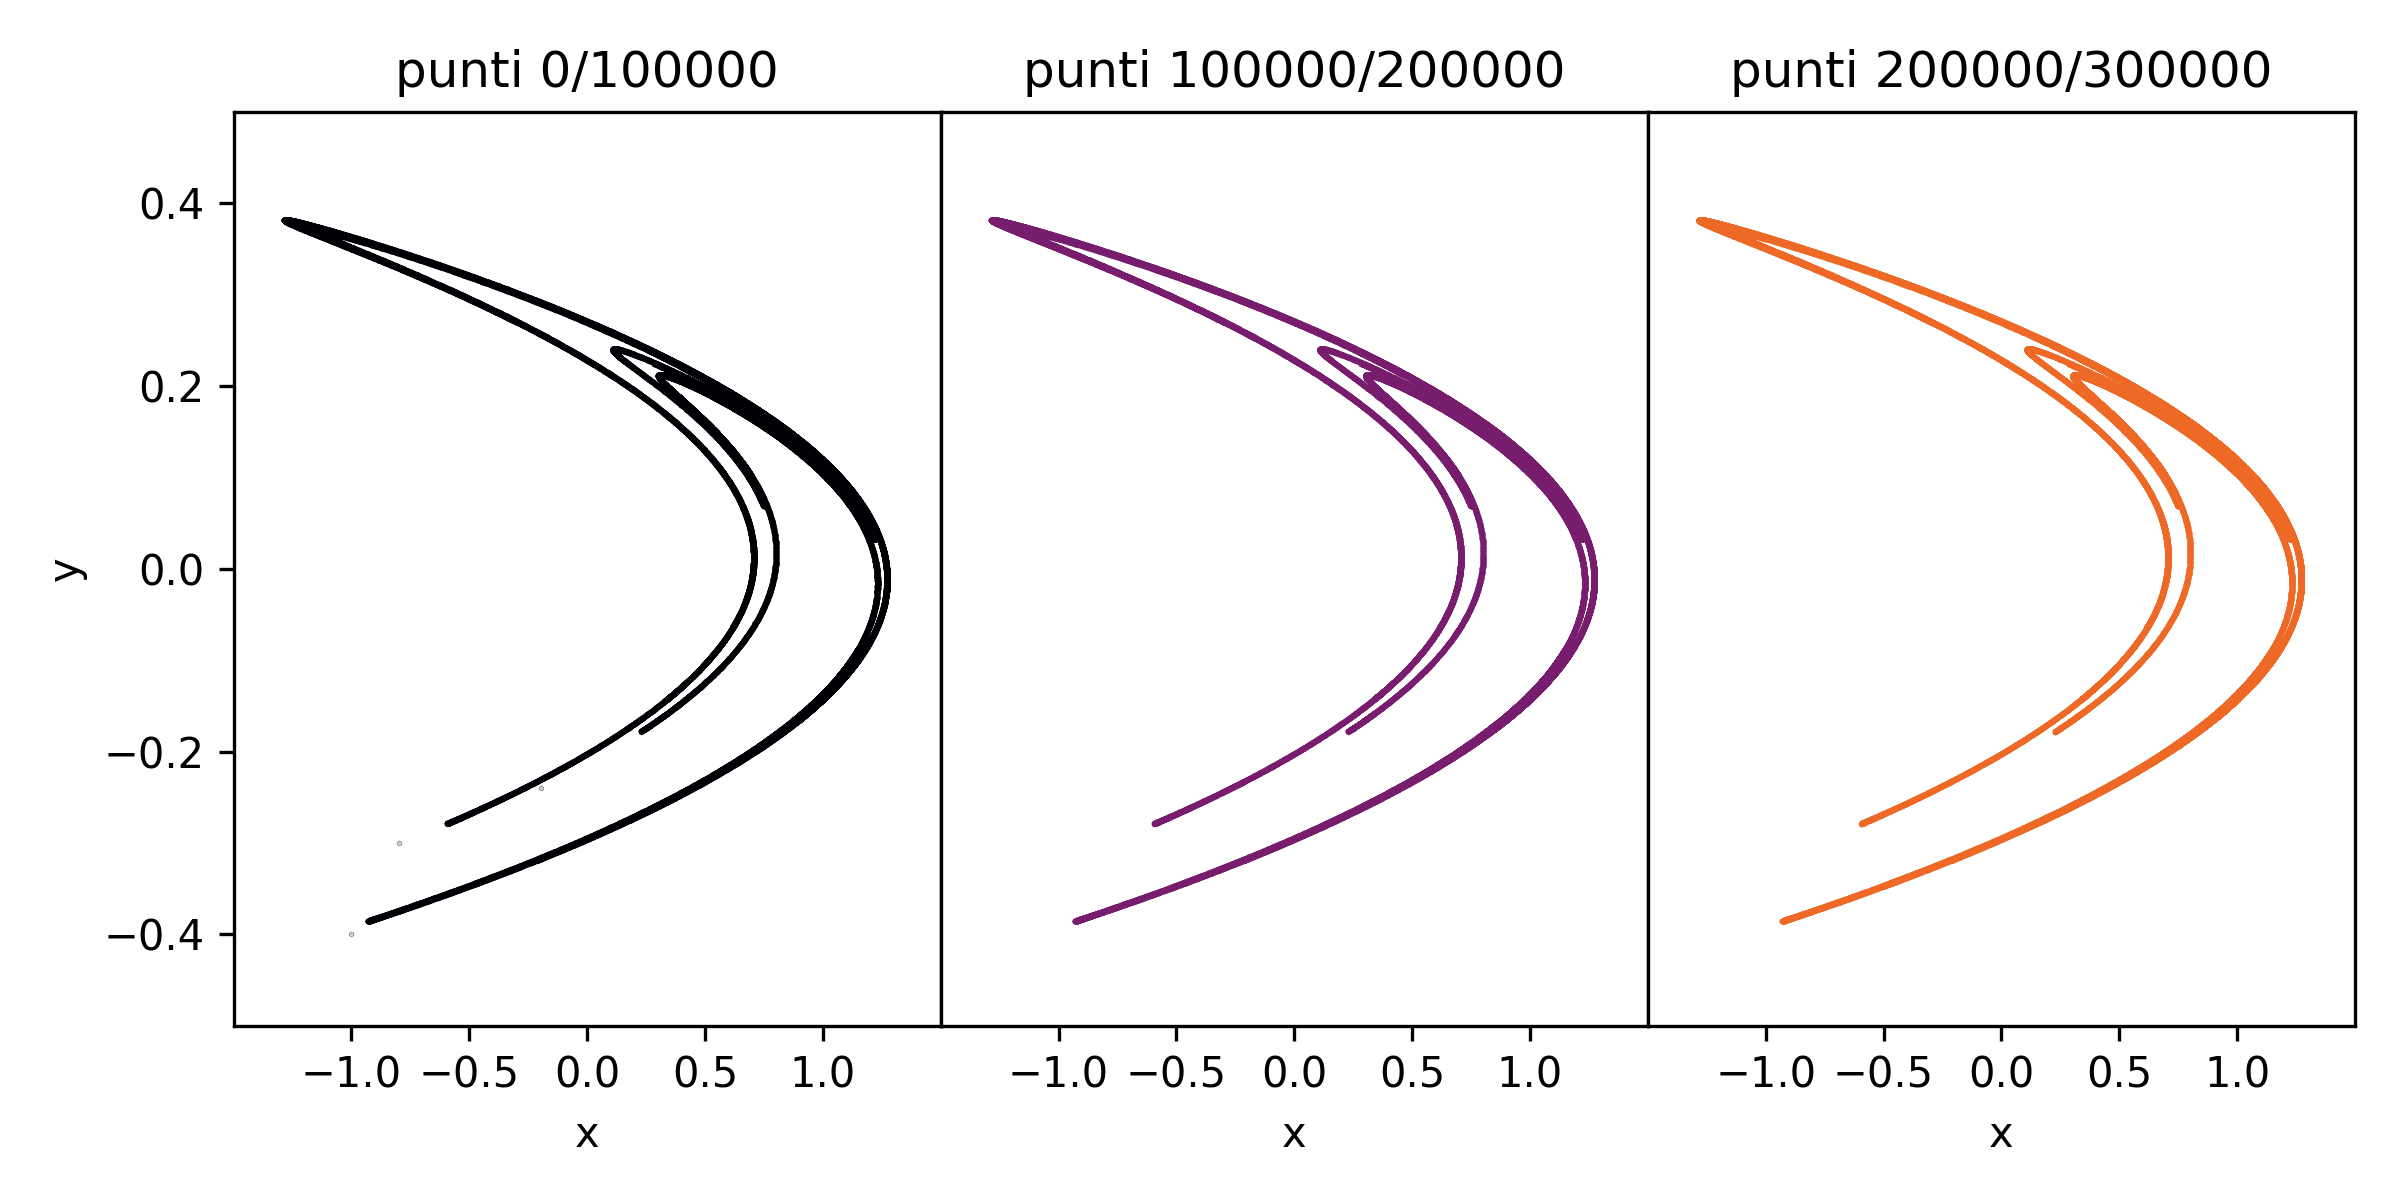
\includegraphics[width=0.45\textwidth]{figures/22_henonmap.png}
	\caption{\scriptsize Mappa di Henon integrata per valori iniziali $(-1, 0.4)$. Si riportano le prime $3\cdot 10^{5}$ iterazioni in 3 blocchi: non cambia nulla dalle prime alle ultime iterazioni. La mappa non doveva contrarre lo spazio delle fasi (che occupa)?}
        \label{fig:figures-22_henonmap-png}
    \end{figure}
\end{exmp}
\noindent
Prima di procedere diamo una importante definizione:
\begin{redbox}{Attrattore}
    Un attrattore è un insieme (set) di punti che attrae la dinamica di un determinato sistema.
\end{redbox}
\noindent
\begin{exmp}[Attrattore di Lorenz]
    Prendiamo la seguente mappa:
    \[
        \begin{cases}
	    \dot{x} = \sigma (y-x)\\
	    \dot{y} = -xz + rx - y \\
	    \dot{z} = xy - bz
        \end{cases}
    .\] 
    I parametri di questo modello sono quantità fisiche, il sistema infatti venne sfruttato per descrivere la fluidodinamica del moto atmosferico da Lorenz. Quest'ultimo voleva dimostrare che nella fluidodinamica atmosferica c'è una forte dipendenza dalle condizioni iniziali.
    \[\begin{aligned}
	&\sigma = \frac{\mu c_p}{k} \\
	&r = \text{num. di Raileigh} \\
	& b = \text{fattore geometrico}
    .\end{aligned}\]
    In cui $\mu$ è la viscosità dell'aria, $c_p$ il suo calore specifico mentre $k$ è la conducibilità. 
    Fisicamente $\sigma$ descrive il meccanismo con cui il sistema può scambiare calore.\\
    Il numero di Rayleigh invece è $>1 (<1)$ se il sistema presenta convezione (conduzione).\\ 
    Per ultimo $b$ è legato al fatto che le ipotesi per questo moto prevedono delle particolari geometrie. \\
    Anche questa mappa assume una forma molto particolare e suggestiva nello spazio delle fasi (Si mostra l'evolvere di una sola condizione iniziale):
    \begin{figure}[H]
        \centering
	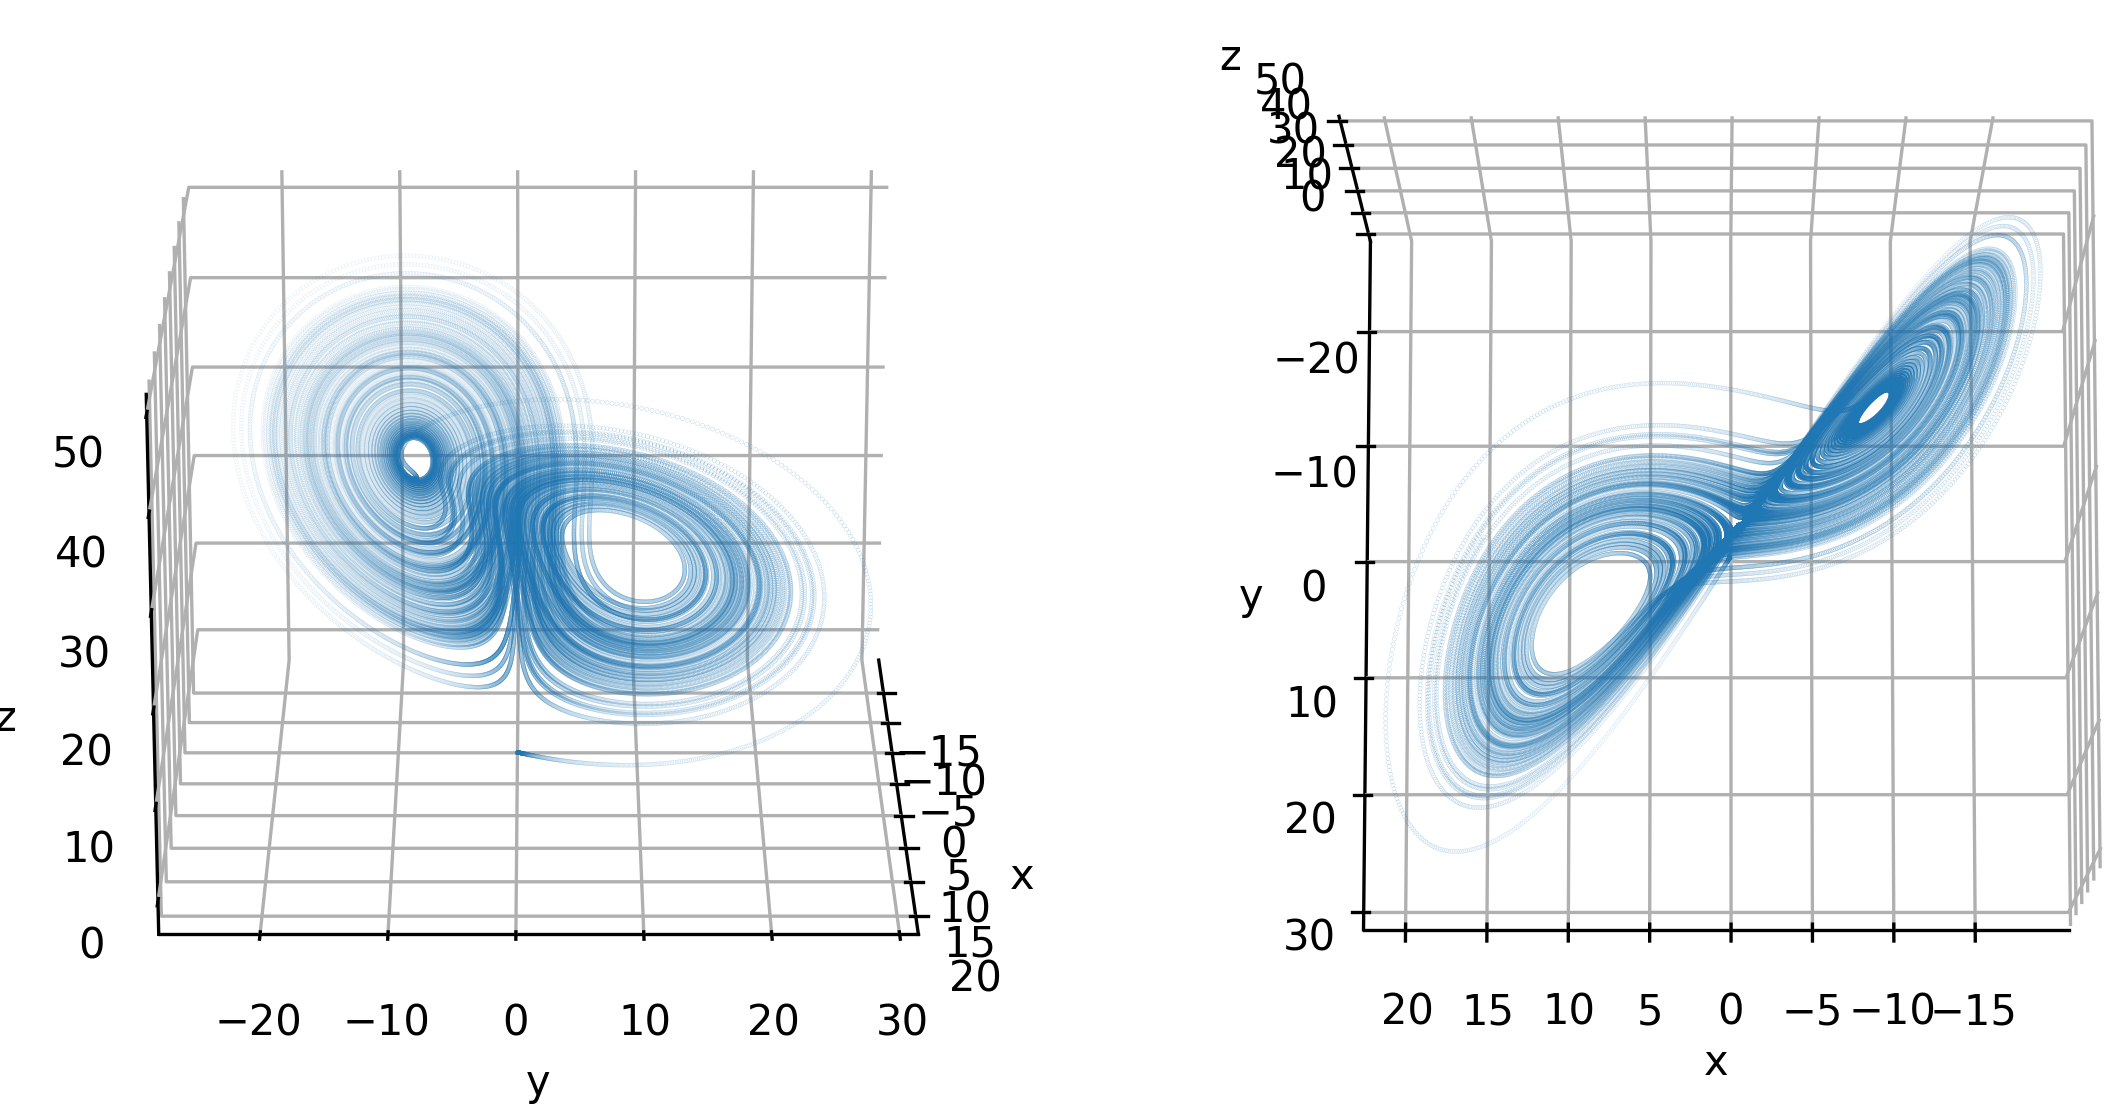
\includegraphics[width=0.45\textwidth]{figures/22_lorenz.png}
        \caption{\scriptsize Attrattore di Lorenz.}
        \label{fig:figures-22_lorenz-png}
    \end{figure}
    Le tre variabili del sistema rappresentano:
    \begin{itemize}
        \item $x$ la convezione del sistema.
	\item $y$ La variazione di temperatura.
	\item La distorsione di $y$ rispetto ad un gradiente lineare di temperatura.
    \end{itemize}
    Quello che fa il modello di Lorenz è descrivere il moto dei fluidi all'interno dei Rolls atmosferici: zone in cui nella parte bassa il fluido è caldo mentre in quella alta il fluido è freddo.\\
    Calcoliamo la "divergenza" della mappa $\nabla \vect{v}$:
    \[
        \nabla \vect{v}  = \frac{\partial }{\partial x} \dot{x} + \frac{\partial }{\partial y} \dot{y} + \frac{\partial }{\partial z} \dot{z} = 
	- (b + \sigma  + 1)
    .\] 
    Quindi visto che $b, \sigma$ sono solitamente maggiori di zero anche questa mappa dovrebbe tendere a collassare nello spazio delle fasi.\\
    Possiamo cercare i punti critici della mappa imponendo che le tre equazioni siano nulle, risolvendo il sistema emergono i seguenti punti:
    \[\begin{aligned}
	& 1)  \ x = y = 0 \\
	& 2) \ y = \pm \sqrt{b (r-1)} \qquad z = r-1 \quad \text{con }r>1
    .\end{aligned}\]
    Possiamo adesso linearizzare le equazioni per valutare la stabilità dei punti fissi, la mappa tangente valutata nel punto $(0, 0, 0)$ ha la struttura:
    \[
        \begin{pmatrix} \delta\dot{x} \\ \delta\dot{y} \\ \delta\dot{z} \end{pmatrix} =
	\begin{pmatrix} 
	    0 & \sigma & -\sigma \\
	    r & -1 & 0\\
	    0 & 0 & -b
	\end{pmatrix} 
	\begin{pmatrix} \delta x\\\delta y\\\delta z \end{pmatrix} 
    .\] 
    Gli autovalori della mappa sono:
    \[\begin{aligned}
	&\lambda_1 = -b\\
	&\lambda_{2, 3} = \frac{-1 \pm \sqrt{1 + 4r\sigma} }{2}
    .\end{aligned}\]
    Il primo autovalore segnala una contrazione poiché $b>0$ quindi $\lambda_1<0$. Per quanto riguarda la coppia $\lambda_{2, 3}$ si ha che sicuramente $\lambda_2$ (quello con il $+$ ) è positivo (se $4r\sigma  > 0$), quindi l'origine potrebbe essere un punto iperbolico.	\\
    Per quanto riguarda il secondo punto fisso invece tralasciamo il conto, il risultato che si ottiene è:
    \[\begin{aligned}
	&\lambda_1 < 0\\
	& \lambda_{2,3} = \alpha\pm i\beta
    .\end{aligned}\]
    Gli autovalori complessi coniugati hanno la particolarità che $\alpha$ cambia di segno per il seguente valore di $r$:
    \[
	\overline{r} = \frac{\sigma  (\sigma  + b + 3)}{\sigma-b-1}
    .\] 
    Quando $\alpha$ assume valori negativi ($r<\overline{r}$) l'oggetto rilassa nel punto fisso, viceversa abbiamo un punto fisso di tipo spirale instabile.
\end{exmp}
\noindent
Il problema che non riusciamo al momento a spiegarci non è il fatto che questi oggetti continuino nel loro moto nello spazio delle fasi, quello che non si riesce a spiegare è il fatto che gli oggetti sembrano continuare a muoversi senza un vincolo. \\
Se pensiamo al pendolo forzato con una forzante periodica abbiamo che la forzante vincolerà il pendolo a fare un moto completamente determinato, quindi di fatto è come se il sistema avesse perso un grado di libertà. \\ 
Con l'attrattore di Lorenz non si riesce a fare il medesimo ragionamento perché il moto sembra continuare a vivere in tutte e tre le dimensioni dello spazio delle fasi.\\
Per spiegare questi fenomeni dobbiamo introdurre dei nuovi concetti: 
\subsection{Il concetto di frattale}%
\label{sub:Il concetto di frattale}
La regola che ne emerge è che data una misura di una quantità $m$ in una determinata scala $l$, una nuova misura $m'$ effettuata con scala $l'$ che sia $N$ volte più piccola di $l$ è legata alla dimensionalità $D$ del sistema nel seguente modo:
\[
    m' = m\cdot N^D 
.\] 
\begin{figure}[H]
    \centering
    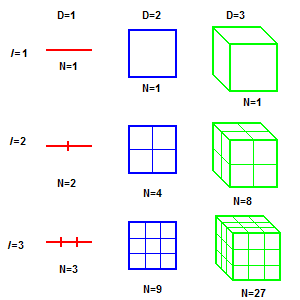
\includegraphics[width=0.3\textwidth]{figures/fractal_wiki.png}
    \caption{\scriptsize Concetto di misura e dimensionalità (wikipedia)}
    \label{fig:figures-fractal_wiki-png}
\end{figure}
\noindent
Quindi il rapporto tra due scale differenti va come:
\[
    \frac{m'}{m} = N^D
.\] 
Chiamando $p$ il rapporto tra le due misure possiamo invertire quest'ultima relazione per ottenere una buona definizione della dimensionalità del sistema $D$:
\begin{redbox}{Dimensione frattale}
\begin{equation}
    D = \frac{\ln p}{\ln N}
    \label{eq:22_dim_fratt}
\end{equation}
\end{redbox}
\noindent
La cosa importante da notare è la generalità della definizione, così generale che appare una cosa controversa: nessuno ci garantisce che $D$ sia intero in quella formula!
\begin{exmp}[Fiocco di Koch]    
Noto questo concetto prendiamo un esempio "pratico". Muniamoci di uno strumento di misura che ha una scala $l$, cerchiamo di adoperarlo per misurare il perimetro di un oggetto che, su questa scala, appare triangolare.
\begin{figure}[H]
    \centering
    \incfig{22_triangolo}
    \caption{\scriptsize triangolo del quale vogliamo misurare il perimetro con la scala più grande.}
    \label{fig:22_triangolo}
\end{figure}
\noindent
Il perimetro misura con questa prima scala $3l$. 
Adesso proviamo a misurarlo con uno strumento avente scala $l /3$, scopriamo che l'oggetto aveva in realtà una forma leggermente diversa:
\begin{figure}[H]
    \centering
    \incfig{22_koch}
    \caption{\scriptsize La struttura si presenta in modo sempre più complicato al rimpicciolire della scala di osservazione.}
    \label{fig:22_koch}
\end{figure}
\noindent
Allora la misura del perimetro diventa (figura \ref{fig:22_koch} a sinistra) $3\cdot 4\cdot l$, diverso dal valore che ci saremmo aspettati per il triangolo "smooth": $3\cdot 3\cdot l$.\\
Iterando ancora il ragionamento la struttura successiva è quella di figura \ref{fig:22_koch} a sinistra: abbiamo un perimetro di $3 \cdot 4\cdot 4 l$.\\
Diventa subito evidente che, se il sistema continua a fare questo scherzetto su tutte le scale, la misura di $D$ per questo esempio ci porta a concludere qualcosa di strano:
\[
    D = \frac{\ln 4}{\ln 3}
.\] 
Otteniamo una dimensionalità che sta a metà tra una superficie ed una linea!\\
Questo sistema è un famosissimo sistema frattale chiamato fiocco di Koch, la struttura "finale" ricorda appunto un fiocco di neve.
\end{exmp}
\noindent
Di insiemi frattali ne esistono tantissimi, solitamente producono tutti effetti grafici mozzafiato ed hanno spesso utilità nel campo dell'"image recognition".\\
Citiamo alcuni esempi di insiemi famosi:
\begin{itemize}
    \item Set di Cantor.
    \item Mandelbrot.
    \item Triangolo di Sierpinski.
    \item Julia.
\end{itemize}
Tornando ai nostri attrattori e le mappe non Hamiltoninane, possiamo definire:
\begin{greenbox}{Attrattore frattale}
    Quando la contrazione di un sistema nello spazio delle fasi incontra strutture sempre più complesse durante la contrazione allora il sistema non si arresta ma continua nel moto.
\end{greenbox}
\noindent
Nei due esempi esaminati sopra (Henon, Lorenz) succede esattamente questo. Questo è il motivo per cui la dinamica non si arresta.
\subsection{Algoritmo di Box Counting per stimare la dimensione frattale}%
\label{sub:Algoritmo di Box Counting per stimare la dimensione frattale}
Prendiamo un esempio che abbiamo già esaminato ma del quale non conosciamo la dimensione frattale: la mappa di Henon. \\
L'idea è quella di suddividere lo spazio delle fasi in quadranti in modo ricorsivo. Per ognuno di questi quadranti si cerca di verificare se sono presenti punti della mappa all'interno.
\begin{figure}[H]
    \centering
    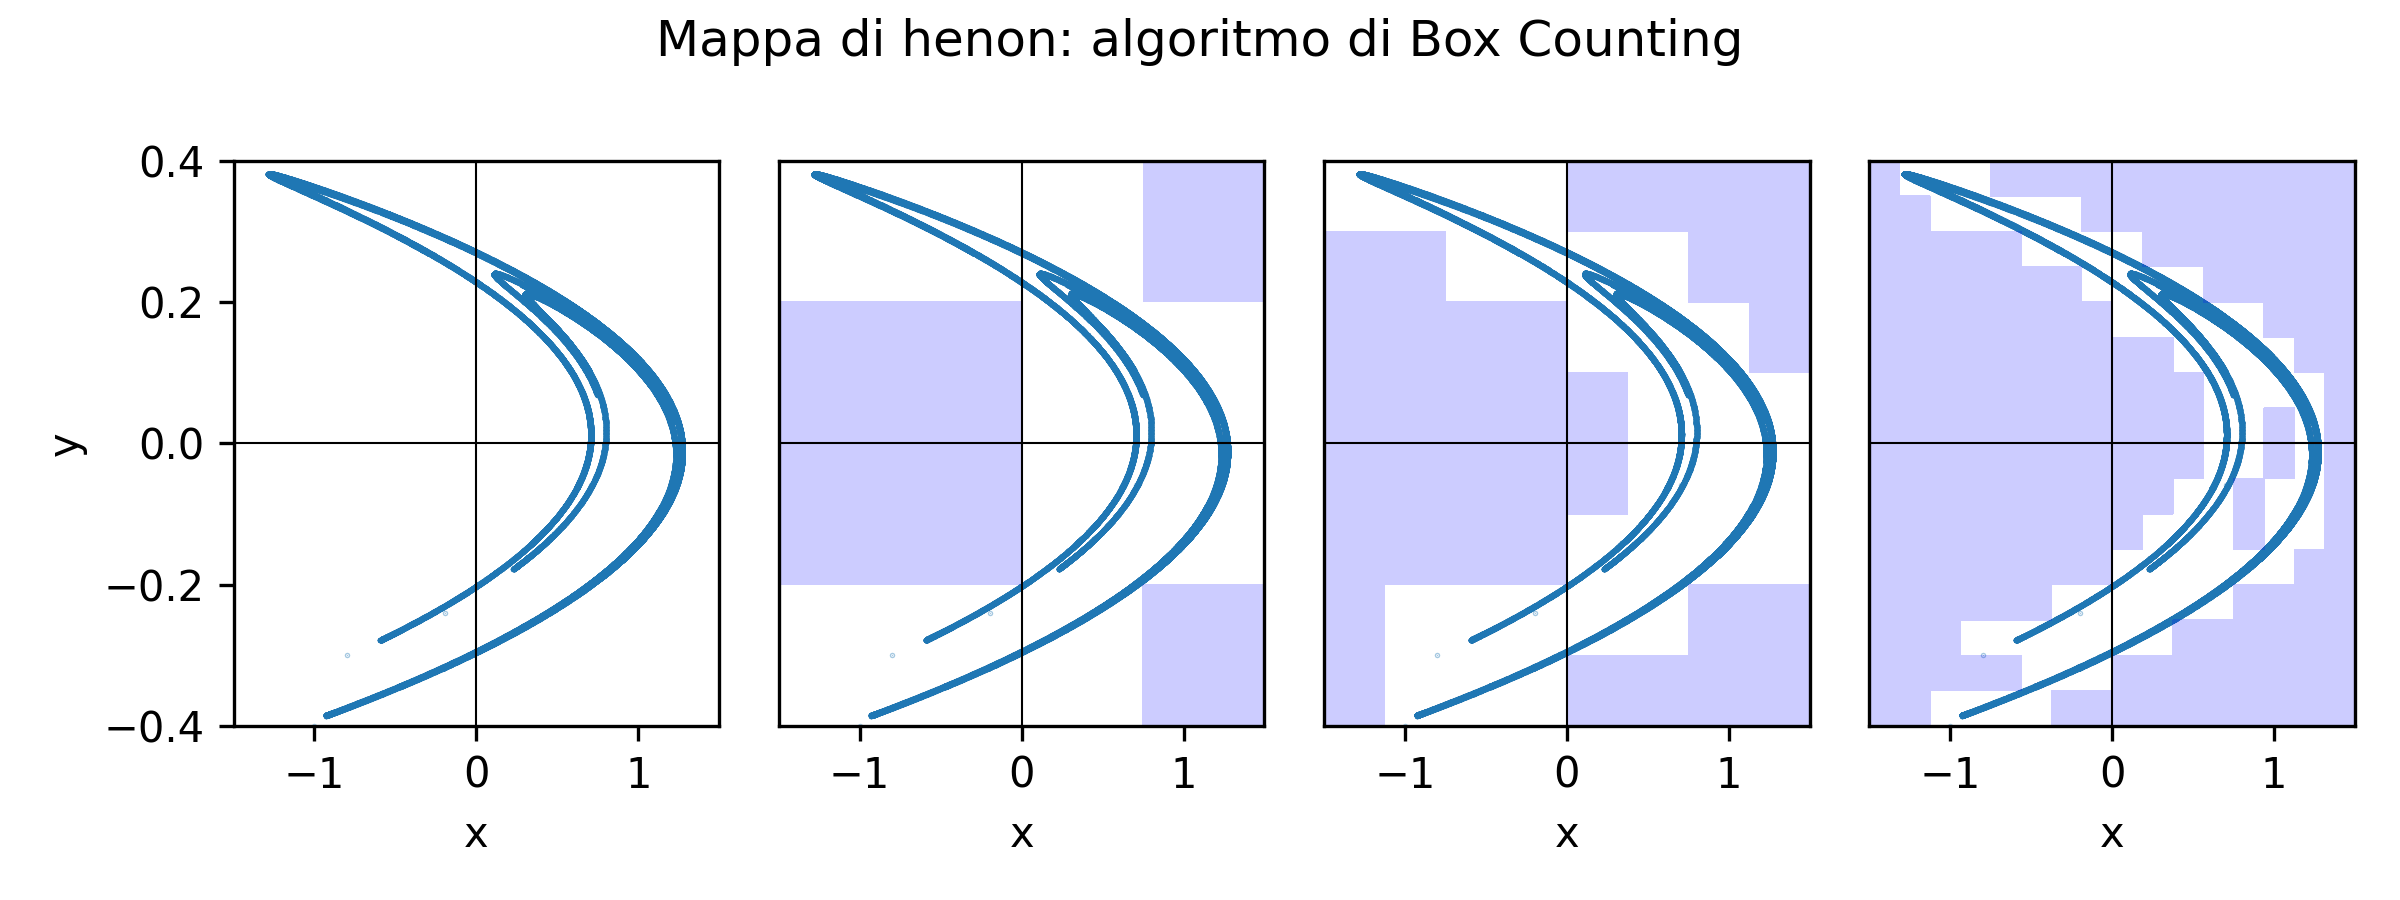
\includegraphics[width=0.45\textwidth]{figures/22_henonmap_box.png}
    \caption{\scriptsize Quadranti sempre più piccoli occupati dai punti della mappa.}
    \label{fig:figures-22_henonmap_box-png}
\end{figure}
\noindent
In conclusione si valuta quanti quadrati sono occupati rispetto alla suddivisione scelta (una potenza di ($1 /2$)).
\begin{itemize}
    \item $1 /2 \to 4$.
    \item $1 /4 \to 10$.
    \item $1 /8 \to 27$.
\end{itemize}
Procedendo in questo modo e continuando a dividere lo spazio in quadrati sempre più piccoli possiamo trovare la dimensione del sistema con la formula \ref{eq:22_dim_fratt}.\\
In questo caso $N$ è proprio il numero che sta al denominatore per l'elenco sopra (2, 4, 8\ldots).\\
Effettuando varie misure di $p$ (il numero di quadrati occupati) al variare di $N$ ed effettuando un fit lineare in $\ln (N), \ln (p)$ si ottiene:
\begin{figure}[H]
    \centering
    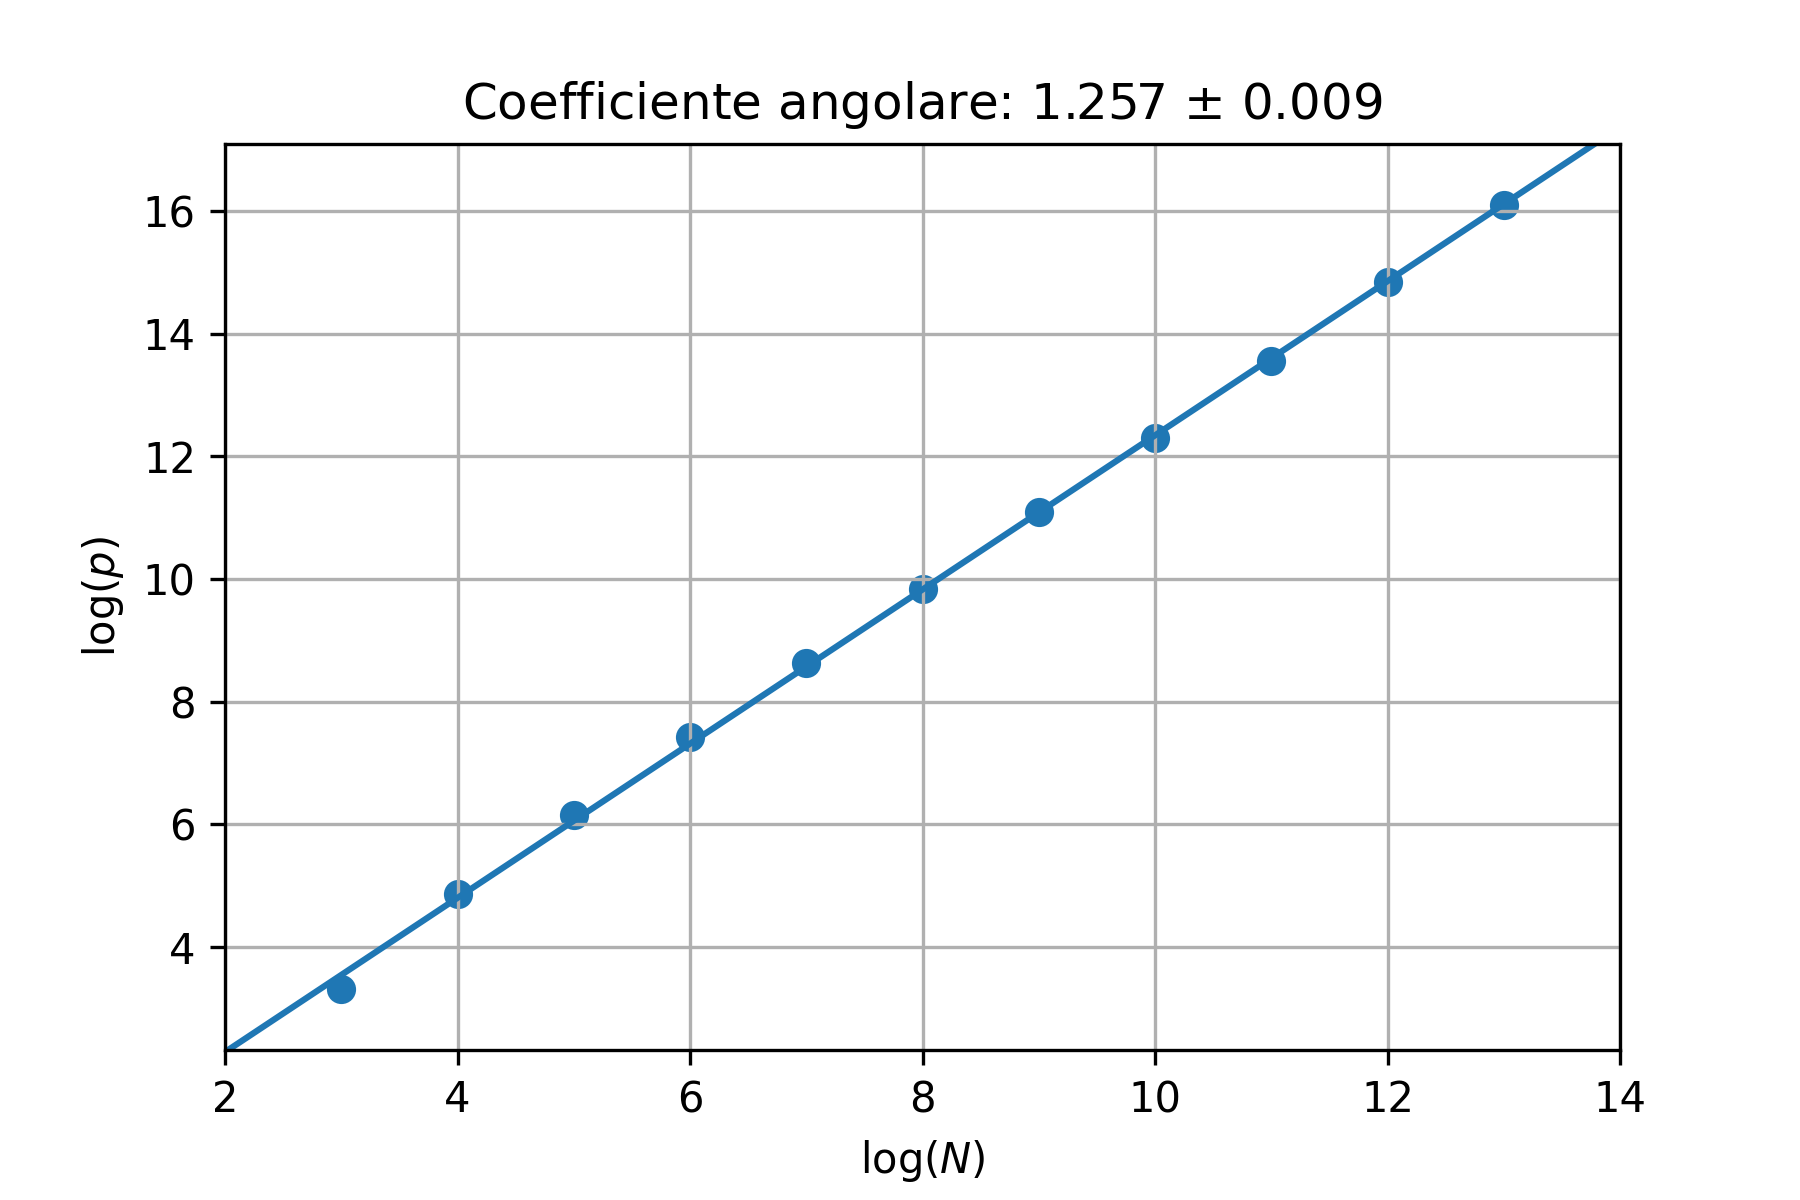
\includegraphics[width=0.5\textwidth]{figures/22_box_fit.png}
    \caption{\scriptsize Fit lineare: la conclusione del metodo di Box counting. \\
    Il coefficiente angolare rappresenta la dimensionalità del sistema ed il logaritmo è in base 2.\\
    I numeri sugli assi non ci permettono di apprezzare il costo computazionale di questa operazione\ldots}
    \label{fig:figures-22_box_fit-png}
\end{figure}
\noindent
Si ottiene una dimensione frattale compatibile con quella scritta da Wikipedia per il sistema: $1.25 \pm 0.02$.\\
Lo stesso metodo può essere applicato all'attrattore di Lorenz, semplicemente in tal caso è necessario usare come scala un cubo (la mappa è 3D).
Nel caso di Lorenz emerge anche un altro problema: la dimensionalità costa computazionalmente. \\
Il metodo di ricerca da me implementato si basa sul metodo della "rubrica telefonica" ed è scritto in python: in due dimensioni inizia già ad accusare (3 secondi per il grafico sopra). Per fare una cosa tridimensionale forse è giusto lasciare il posto a linguaggi più performanti (quando si tratta di loop) come fortran.\\
Consiglio di dare un occhio tra i codici poiché l'algoritmo che ho pensato per implementare la ricerca elude il problema del dover creare una matrice enorme per avere una "buona risoluzione" dello spazio delle fasi\ldots\\
Perché è così importante studiare la dimensione frattale? Perché c'è un teorema che afferma una cosa sconvolgente:
\begin{redbox}{Teorema Caos-frattale}
    Se un sistema presenta una dimensione frattale non intera allora il sistema è caotico.
\end{redbox}
\noindent
Quindi semplicemente applicando un box counting potremmo dimostrare che il sistema è caotico, senza dover passare dagli altri metodi visti nelle precedenti lezioni.\\
\subsection{Mappa di Henon come meccanismo di Folding e Stretching}%
\label{sub:Mappa di Henon come meccanismo di Folding e Stretching}
La mappa di Henon può esser vista anche come la composizione di 3 mappe distinte, queste tre mappe vengono applicate in successione ad ogni step:
\[
    \begin{cases}
        \overline{x} = x\\
	\overline{y} = y + 1 - a\overline{x}^2
    \end{cases}
\] 
Questa prima mappa trasporta i punti verso una parabola.
\begin{figure}[H]
    \centering
    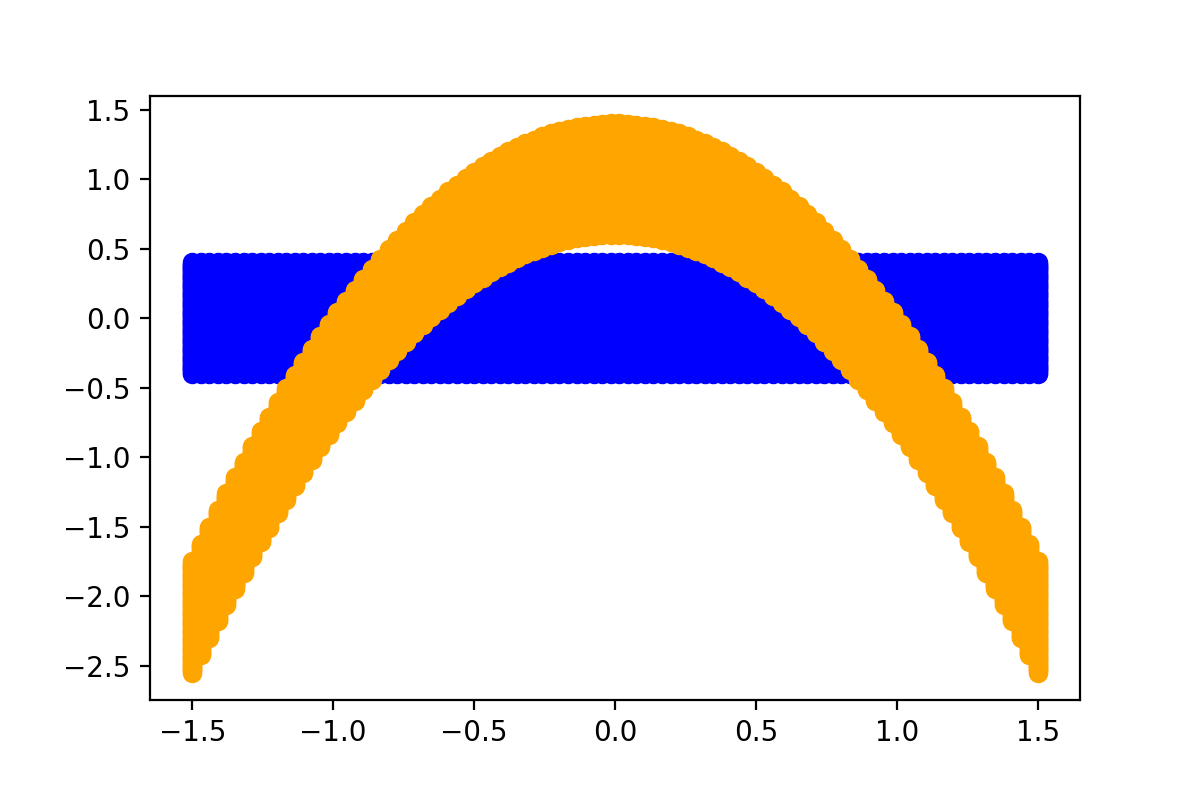
\includegraphics[width=0.3\textwidth]{figures/22_step1henon.png}
    \caption{\scriptsize Prima mappa}
    \label{fig:figures-22_step1henon-png}
\end{figure}
\noindent
La seconda mappa invece comprime i punti sull'asse x:
\[
    \begin{cases}
        \overline{\overline{x}} = b\overline{x}\\
	\overline{\overline{y}} = \overline{y}
    \end{cases}
\] 
\begin{figure}[H]
    \centering
    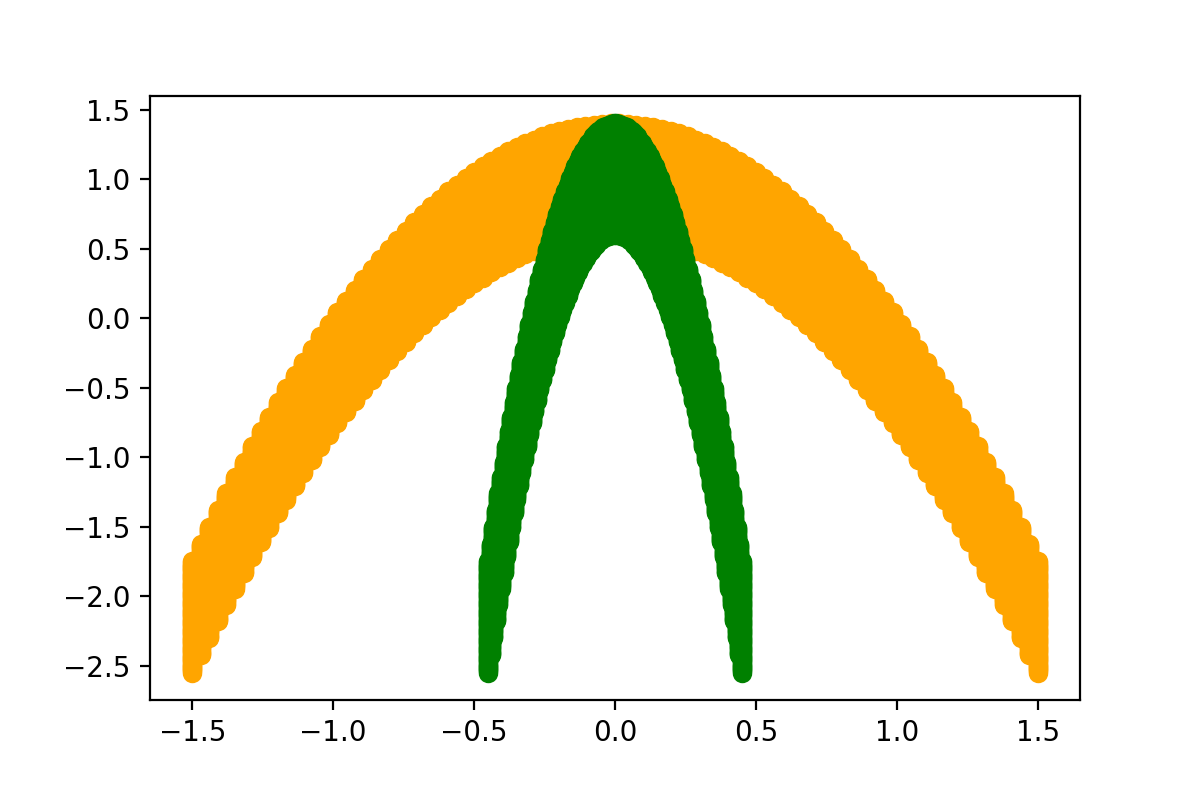
\includegraphics[width=0.3\textwidth]{figures/22_step2henon.png}
    \caption{\scriptsize seconda mappa}
    \label{fig:figures-22_step1henon-png}
\end{figure}
\noindent
In conclusione abbiamo una riflessione sulla bisettrice del primo quadrante.
\[
    \begin{cases}
        \overline{\overline{\overline{x}}} = \overline{\overline{y}}\\
	\overline{\overline{\overline{y}}} = \overline{\overline{x}}
    \end{cases}
\] 
\begin{figure}[H]
    \centering
    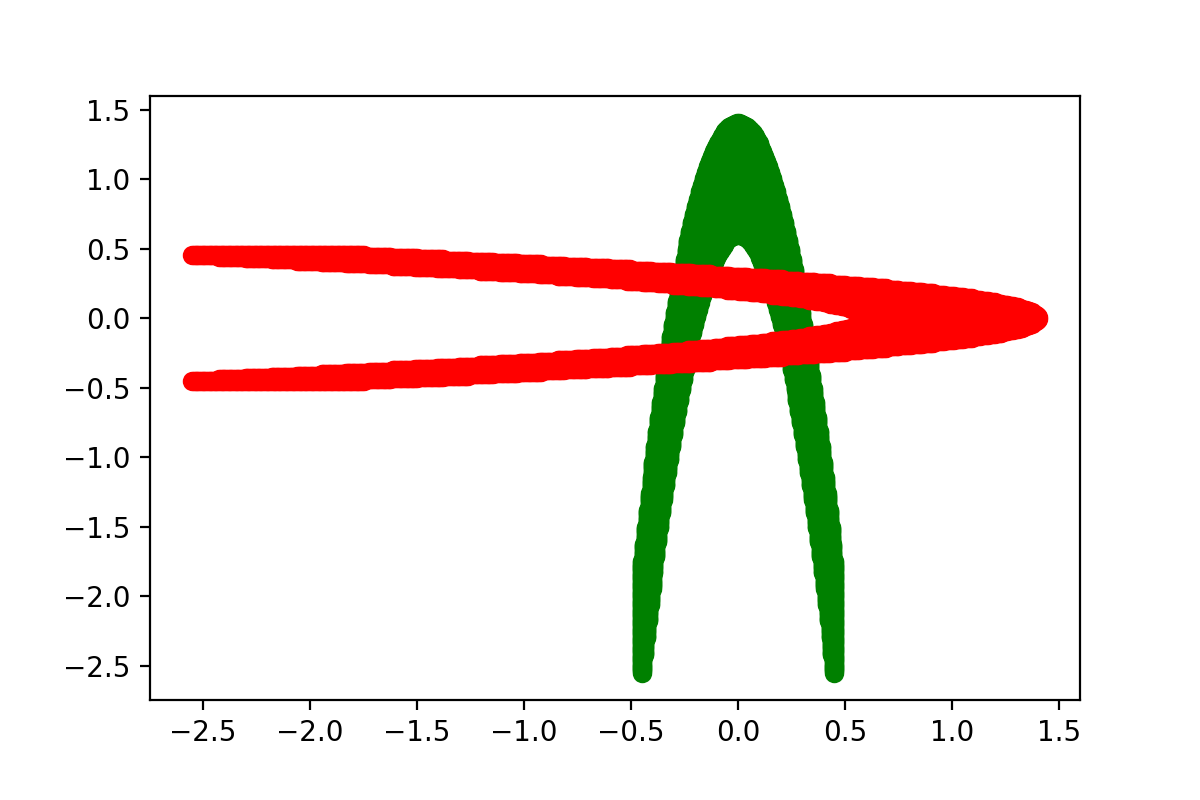
\includegraphics[width=0.3\textwidth]{figures/22_step3henon.png}
    \caption{\scriptsize Terza mappa}
    \label{fig:figures-22_step1henon-png}
\end{figure}
\noindent
\clearpage

\section{Lezione 23}%
\label{sub:Lezione 23}


\section{Attrattore di Lorenz}%
\label{sec:Lezione 24}
\mylocaltoc
\subsection{Nozioni di fluidodinamica}%
\label{sub:Nozioni di fluidodinamica}
\subsubsection{Equazione di diffusione}%
\label{subsub:Equazione di diffusione}
Prendiamo un sistema fluido in cui è presente un gradiente di temperatura $\Delta T$ in una distanza nella coordinata $z$ data da $h$:
\[
    \Delta T = \frac{T_1-T_0}{h}\Delta z
.\] 
Studiamo il processo di diffusione termica in un cubetto infinitesimo di materia tra il piano $z=0$ e $z=h$. Il calore entrante nel cubetto è $Q_d$, quello uscente è $Q_u$.
\[\begin{aligned}
    \Delta Q =& - Q_u+Q_d \propto\\
    \propto & \ D_T (-T(\Delta z)+T(0) - T(-\Delta z)) \propto\\
    \propto & \ D_T \nabla ^2T
.\end{aligned}\]
Quindi, visto che il gradiente di temperatura in $z$ per il cubetto è sempre $\Delta T$ abbiamo l'equazione di diffusione del calore nel materiale:
\[
    \frac{\text{d} T}{\text{d} t} = \frac{\partial T}{\partial t}  + \vect{v}\nabla T = D_T \nabla ^2T
.\] 
\subsubsection{Forze in gioco nel sistema}%
\label{subsub:Forze in gioco nel sistema}
Visto che il sistema è un fluido subirà la spinta di Archimede, questa spinta è dovuta al gradiente di temperatura che indurrà una dilatazione termica:
\[
    g\Delta V(\rho_0 + \alpha\rho_0\Delta T- \rho_0)
.\] 
In cui $\alpha$ è il coefficiente di dilatazione termica, $\Delta V$ è l'unità di volume (rappresentata dal volume del cubetto).
\[
    \frac{F_A}{\Delta V} = g\rho_0\alpha\frac{T_1-T_0}{h}\Delta z
.\] 
Sentirà anche le forze viscose. Per valutare immaginiamo di traslare il piano superiore del sistema di un fattore $\Delta z$ a velocità costante $\Delta v$ rispetto al piano inferiore. La forza necessaria per effettuare questa operazione può essere modellizzata come:
\[
    F(z + \Delta z) = \mu  \frac{\Delta v}{\Delta z}A
.\] 
In cui $\mu$ è il coefficiente di viscosità, $A$ la superficie da traslare.\\
La velocità $\Delta v$ rappresenta la velocità relativa tra i due piani che stiamo considerando.\\
Possiamo valutare un gradiente di forza per effettuare la traslazione calcolando $F(z+\Delta z)-F(z)$:
\[
    f = F(z+\Delta z)-F(z)= \frac{\partial F}{\partial z} \Delta z = \mu\frac{\partial^2v}{\partial z^2} A\Delta z
.\] 
In conclusione, come per Archimede, prendiamo la forza per unità di volume:
\[
    F_v = \frac{f}{\Delta V} \implies \frac{f_i}{A\Delta z} = \mu\nabla ^2v_i
.\] 
in cui $i$ sta ad indicare la coordinata $i$-esima della forza $(x,y,z)$.\\
Visto che la distanza delle due piastre è $h$ possiamo approssimare il $\nabla ^2v$ come:
\[
    F_{v,z} = \mu \frac{v_z}{h^2}
.\] 
Notiamo che nelle equazioni delle forze e di diffusione vi sono delle importanti quantità intensive del fluido in considerazione
\[
    \left[\rho\right] = \frac{\left[M\right]}{\left[L\right]^3} \qquad
    \left[D_T\right] = \frac{\left[L\right]^2}{\left[T\right]}\qquad
    \left[\mu\right] = \frac{\left[M\right]}{\left[L\right]\left[T\right]}
.\] 
è utile introdurne altre, come la \textbf{Viscosità cinematica}:
\[
    \nu  = \frac{\mu}{\rho} = \frac{\left[L\right]^2}{\left[T\right]}
.\] 
Questa è legata alle forze tra le molecole del fluido (come è lecito aspettarsi avendo al denominatore la densità).\\
In questo modo si ha una quantità che può essere sfruttata sia per studiare i fluidi che per studiare i gas.\\
Introduciamo anche un numero puro, rilevante per il nostro sistema: il \textbf{Numero di Prandtl}.
\[
    P = \frac{\nu}{D_T}
.\] 
Questo misura l'importanza relativa tra viscosità e diffusione termica.\\
\subsubsection{Equilibrio tra forze e scale tipiche temporali}%
\label{subsub:Equilibrio tra forze}
Uguagliando la forza di Archimede a quella viscosa:
\begin{equation}
    \alpha\rho_0g \frac{\Delta T}{h} \Delta z = \mu  \frac{v}{h^2}
    \label{eq:24_eq}
\end{equation}
Se abbiamo un oggetto che rompe l'equilibrio (perché troppo caldo ad esempio) allora inizierà a salire lungo l'asse $z$ fino a raggiungere una velocità uniforme di salita: l'equilibrio tra Archimede e la forza viscosa.\\
Questo fenomeno definisce una velocità limite che può essere ottenuto invertendo la relazione \ref{eq:24_eq}.
\[
    v_{lim} = \frac{\alpha\rho_0g\Delta T\Delta zh}{\mu}
.\] 
In presenza di questa velocità limite l'oggetto del moto percorre una distanza $\Delta z$ in un tempo critico $\tau_{v}$  determinato dall'equilibrio stesso:
\[
    \frac{\Delta z}{v_{lim}} = \frac{\mu}{\alpha\rho_0g\Delta T\Delta zh} = \tau_{v}
.\] 
Questo tempo è legato a quanto tempo impieghiamo a portare in equilibrio il sistema con il moto convettivo.\\
L'equilibrio potrebbe essere raggiunto anche tramite un processo di diffusione.
\[
    \partial_{t}T\sim D_T\nabla ^2T \sim D_T \frac{T}{h^2} \implies  \tau_{T} = \frac{h^2}{D_T}
.\] 
Valutando il rapporto tra le scale temporali di diffusione e di convezione otteniamo un altro numero puro: il \textbf{numero di Rayleigh}.
\[
    R_a = \frac{\tau_T}{\tau_v} = \frac{h^3}{D_T} \frac{\alpha\rho_0g \Delta T}{\mu}
.\] 
Chiaramente questo numero dice se il sistema è dominato da convezione o da conduzione:
\begin{itemize}
    \item $\tau_T > \tau_v$: stato convettivo.
    \item $\tau_T < \tau_v$: stato non conduttivo.
\end{itemize}
In conclusione abbiamo un ultimo numero puro importante per la dinamica del sistema: il \textbf{Numero di Reynolds}:
\[
    R_e = \frac{\rho vL}{\mu}	
.\] 
In cui $L$ può essere interpretato come il diametro del "tubo" in cui avviene il moto.\\
Questo numero misura la transizione tra un fluido di tipo laminare ($R_e < 1000$ ) ed un fluido di tipo turbolento ($R_e > 1000$).
\subsection{Modello di Lorenz della turbolenza}%
\label{sub:Modello di Lorenz della turbolenza}
\begin{figure}[H]
    \centering
    \incfig{24_lorenz_turbo}
    \caption{\scriptsize Superfici a temperature $T_{0,1}$ tra le quali è presente un fluido in presenza di gravità.}
    \label{fig:24_lorenz_turbo}
\end{figure}
Ipotizziamo di avere un fluido incomprimibile come in figura \ref{fig:24_lorenz_turbo} con le seguenti caratteristiche note:
\begin{itemize}
    \item $\rho_0$ a temperatura $T_0$.
    \item $\nu = \mu  /\rho_0$ coefficiente di viscosità cinematica.
    \item $\alpha$ coefficiente di espansione termica.
    \item $D_T$ coefficiente di diffusione.
\end{itemize}
Cerchiamo il campo di velocità del fluido $\vect{u}$. Le componenti di questo campo le definiamo come:
\[
    \vect{u}  = (u, v, \omega)
.\] 
Ipotizziamo inoltre che valga la seguente:
\[
    \nabla \vect{u} = 0
.\] 
Diamo per note le equazioni di Navy-Stokes e quelle del gradiente di temperatura:
\[\begin{aligned}
    &\partial_{t}\vect{u} + \vect{u}\nabla \vect{u}  = - \frac{1}{\rho_0}\nabla P + \nu\nabla ^2\vect{u} + \alpha g(T-T_0)\hat{z}\\
    & \partial_{t}T + \vect{u}\nabla T = D_T \nabla ^2T
.\end{aligned}\]
Tradizionalmente si introducono delle variabili riscalate:
\[\begin{aligned}
    &\vect{x}^* = \frac{\vect{x}}{d} && \qquad  t^* = \frac{D_T}{d^2}t\\
    & \vect{u}^* = \vect{u}  \frac{d}{D_T} && \qquad p^* = \frac{1}{\rho_0}\left(\frac{d}{D_T}\right)^2P\\
    & \theta^* = \frac{T-T_0}{T_1-T_0}-z^* && \qquad \left[T = T_0 + \Delta T(\theta^*+z^*)\right]
.\end{aligned}\]
La variabile $\theta^*$ rappresenta la variazione dalla linearità del profilo di temperatura.\\
Inserendo queste variabili nelle equazioni sopra:
\[\begin{aligned}
    & \nabla \vect{u}  = 0\\
    & \partial_{t}\vect{u}  + \vect{u}\cdot \nabla \vect{u} = - \nabla P + P_r \nabla ^2\vect{u} + P_rR_a \theta \hat{z}\\
    &\partial_{t}\theta + \vect{u}\cdot \nabla \theta = \omega + \nabla ^2\theta
.\end{aligned}\]
In cui $P_r = \nu  /D_T$. \\
Inseriamo le condizioni al contorno:
\[
    z = 0, 1 
    \qquad 
    \theta  = 0
    \qquad
    \omega = 0
    \qquad
    \frac{\partial ^2\omega}{\partial t^2}  = 0
.\] 
Fino a questo punto il problema è piuttosto generale, Lorenz lo specializzò ad una situazione particolare: il fluido deve muoversi su dei rulli ("rolls").
\begin{figure}[H]
    \centering
    \incfig{24_rolls}
    \caption{\scriptsize Moto del fluido tra i due strati, si ipotizza quindi la componente della velocità $\vect{u}_x$ nulla.}
    \label{fig:24_rolls}
\end{figure}
In questo modo ci si riduce a studiare il moto solo lungo il piano $y, z$. La divergenza nulla del campo di velocità implica allora che:
\[
    \partial_{y}u_y + \partial_{z}u_z = 0
.\] 
Una ipotesi (forte) che possiamo fare è che la forma del campo di velocità sia del seguente tipo:
\[
    u_y = \partial_{z}\psi (y,z) \qquad u_z = -\partial_{y}\psi (y,z)
.\] 
In questo modo la divergenza nulla è rispettata. La funzione $\psi$  viene chiamata "stream function". \\
Quest'ultima ipotesi equivale a dire che il rotore del campo di velocità (la vorticità: $\vect{\xi}$) sia solo lungo $x$.
\[
    \vect{\xi}  = \nabla \times \vect{u}  \implies  \xi_x = \partial_{y}u_z - \partial_{z}u_y = - \nabla_2^2\psi
.\] 
In cui l'ultimo laplaciano $\nabla^2_2$  è bidimensionale.\\
Facendo il rotore della equazione di Navy-Stokes nelle variabili riscalate possiamo introdurvi la $\vect{\xi}$. Effettuando un pò di algebra si arriva alla seguente espressione:
\[
    \frac{\partial \xi}{\partial t} + \vect{u}\nabla \xi = P_r \nabla ^2_2 \xi + P_r R_a \frac{\partial \xi}{\partial y} 
.\] 
L'equazione per la variabile $\theta$  invece può essere riscritta come:
\[
    \frac{\partial \theta}{\partial t}  + J(\theta,\psi) = \nabla _2^2\xi - \frac{\partial \xi}{\partial y} 
.\] 
Dove si definisce la quantità:
\[
    J(f, \psi) = \vect{u}\nabla f
.\] 
Grazie alle proprietà della stream function (che entra nella espressione di $J$  sostituendo $u_y, u_z$). \\
In conclusione il sistema di equazioni differenziali da risolvere diventa:
\[\begin{aligned}
    & \xi = - \nabla _2^2\psi\\
    & \frac{\partial \xi}{\partial t} + J(\xi, \psi) = P_r \nabla ^2_2 \xi + P_r R_a \frac{\partial \xi}{\partial y} \\
    &\frac{\partial \theta}{\partial t}  + J(\theta,\psi) = \nabla _2^2\xi - \frac{\partial \xi}{\partial y} 
.\end{aligned}\]
Queste ci determinano completamente il moto nei rolls.\\
A questo punto viene fatta una approssimazione \\
A questo punto viene fatta una approssimazione sfruttando l'espansione di Galerkin. Si cercano i modi più bassi che possono essere rilevanti per la dinamica che vogliamo studiare.
\[\begin{aligned}
    & \psi (z, y, t) = a(t)\sin (\pi z)\sin (k\pi y)\\
    & \theta (z, y, t) = b(t)\sin (\pi z) \cos (k\pi y) + c(t)\sin (2\pi z)
.\end{aligned}\]
I termini trigonometrici in $k\pi y$ tengono di conto della periodicità del moto sui rolls, i termini che contengono invece $\pi z$  tengono di conto che il moto può dipendere dall'angolo.\\
A questo punto si reinseriscono queste quantità nelle equazioni differenziali ed otterremo un sistema di equazioni nelle derivate rispetto al tempo dei coefficienti $a, b, c$. \\
In particolare i termini $a, b$  rappresentano  dei rolls lungo $y$ (aventi numero d'onda $k$). La variabile $c$ invece tiene di conto della convezione e quantifica la deviazione della temperatura rispetto alla media.\\
Il risultato finale di questa operazione sono le seguenti 3 equazioni:
\[\begin{aligned}
    &\dot{x} = -\sigma x + \sigma  y\\
    &\dot{y} = -y + rx -xz\\
    & \dot{z} = -\tilde{b}z + xy
.\end{aligned}\]
Con le 3 variabili che sono delle riscalature di $a, b ,c$:
\[\begin{aligned}
    & x = \frac{ka}{\sqrt{2} (1+k^2)}\\
    & y = \frac{kb}{\sqrt{2} (1+k^2)}\\
    & z = c
.\end{aligned}\]
Le equazioni scritte sopra sono proprio quelle del modello di Lorenz.


\end{document}
